\documentclass[a4paper]{book}
\usepackage{a4wide}
\usepackage{makeidx}
\usepackage{graphicx}
\usepackage{multicol}
\usepackage{float}
\usepackage{listings}
\usepackage{color}
\usepackage{textcomp}
\usepackage{alltt}
\usepackage{times}
\usepackage{ifpdf}
\ifpdf
\usepackage[pdftex,
            pagebackref=true,
            colorlinks=true,
            linkcolor=blue,
            unicode
           ]{hyperref}
\else
\usepackage[ps2pdf,
            pagebackref=true,
            colorlinks=true,
            linkcolor=blue,
            unicode
           ]{hyperref}
\usepackage{pspicture}
\fi
\usepackage[utf8]{inputenc}
\usepackage{doxygen}
\lstset{language=C++,inputencoding=utf8,basicstyle=\footnotesize,breaklines=true,breakatwhitespace=true,tabsize=8,numbers=left }
\makeindex
\setcounter{tocdepth}{3}
\renewcommand{\footrulewidth}{0.4pt}
\begin{document}
\hypersetup{pageanchor=false}
\begin{titlepage}
\vspace*{7cm}
\begin{center}
{\Large InformationTheoryLibrary }\\
\vspace*{1cm}
{\large Generated by Doxygen 1.6.3}\\
\vspace*{0.5cm}
{\small Fri May 20 16:59:07 2011}\\
\end{center}
\end{titlepage}
\clearemptydoublepage
\pagenumbering{roman}
\tableofcontents
\clearemptydoublepage
\pagenumbering{arabic}
\hypersetup{pageanchor=true}
\chapter{Class Index}
\section{Class Hierarchy}
This inheritance list is sorted roughly, but not completely, alphabetically:\begin{DoxyCompactList}
\item \contentsline{section}{ITL\_\-base}{\pageref{classITL__base}}{}
\item \contentsline{section}{ITL\_\-cell$<$ T $>$}{\pageref{classITL__cell}}{}
\begin{DoxyCompactList}
\item \contentsline{section}{ITL\_\-tetrahedron$<$ T $>$}{\pageref{classITL__tetrahedron}}{}
\end{DoxyCompactList}
\item \contentsline{section}{ITL\_\-datastore$<$ T $>$}{\pageref{classITL__datastore}}{}
\item \contentsline{section}{ITL\_\-entropy$<$ T $>$}{\pageref{classITL__entropy}}{}
\item \contentsline{section}{ITL\_\-entropycore}{\pageref{classITL__entropycore}}{}
\item \contentsline{section}{ITL\_\-field$<$ T $>$}{\pageref{classITL__field}}{}
\begin{DoxyCompactList}
\item \contentsline{section}{ITL\_\-field\_\-regular$<$ T $>$}{\pageref{classITL__field__regular}}{}
\item \contentsline{section}{ITL\_\-field\_\-unstructured$<$ T $>$}{\pageref{classITL__field__unstructured}}{}
\end{DoxyCompactList}
\item \contentsline{section}{ITL\_\-globalentropy$<$ T $>$}{\pageref{classITL__globalentropy}}{}
\item \contentsline{section}{ITL\_\-grid$<$ T $>$}{\pageref{classITL__grid}}{}
\begin{DoxyCompactList}
\item \contentsline{section}{ITL\_\-grid\_\-regular$<$ T $>$}{\pageref{classITL__grid__regular}}{}
\item \contentsline{section}{ITL\_\-Grid\_\-unstructured$<$ T $>$}{\pageref{classITL__Grid__unstructured}}{}
\end{DoxyCompactList}
\item \contentsline{section}{ITL\_\-grid\_\-tetrahedral$<$ T $>$}{\pageref{classITL__grid__tetrahedral}}{}
\item \contentsline{section}{ITL\_\-histogram}{\pageref{classITL__histogram}}{}
\item \contentsline{section}{ITL\_\-ioutil$<$ T $>$}{\pageref{classITL__ioutil}}{}
\item \contentsline{section}{ITL\_\-localentropy$<$ T $>$}{\pageref{classITL__localentropy}}{}
\item \contentsline{section}{ITL\_\-localjointentropy$<$ T $>$}{\pageref{classITL__localjointentropy}}{}
\item \contentsline{section}{ITL\_\-statutil$<$ T $>$}{\pageref{classITL__statutil}}{}
\item \contentsline{section}{ITL\_\-util$<$ T $>$}{\pageref{classITL__util}}{}
\item \contentsline{section}{line\_\-2d}{\pageref{structline__2d}}{}
\item \contentsline{section}{MATRIX3}{\pageref{classMATRIX3}}{}
\item \contentsline{section}{MATRIX4}{\pageref{classMATRIX4}}{}
\item \contentsline{section}{VECTOR2}{\pageref{classVECTOR2}}{}
\item \contentsline{section}{VECTOR3}{\pageref{classVECTOR3}}{}
\item \contentsline{section}{VECTOR4}{\pageref{classVECTOR4}}{}
\end{DoxyCompactList}

\chapter{Class Index}
\section{Class List}
Here are the classes, structs, unions and interfaces with brief descriptions:\begin{DoxyCompactList}
\item\contentsline{section}{\hyperlink{classITL__base}{ITL\_\-base} (Base class for the ITL library )}{\pageref{classITL__base}}{}
\item\contentsline{section}{\hyperlink{classITL__cell}{ITL\_\-cell$<$ T $>$} (Cell class representing a unit of an unstructured grid )}{\pageref{classITL__cell}}{}
\item\contentsline{section}{\hyperlink{classITL__datastore}{ITL\_\-datastore$<$ T $>$} (The container class for data )}{\pageref{classITL__datastore}}{}
\item\contentsline{section}{\hyperlink{classITL__entropy}{ITL\_\-entropy$<$ T $>$} (Entropy computation class )}{\pageref{classITL__entropy}}{}
\item\contentsline{section}{\hyperlink{classITL__entropycore}{ITL\_\-entropycore} (Entropy computation core class )}{\pageref{classITL__entropycore}}{}
\item\contentsline{section}{\hyperlink{classITL__field}{ITL\_\-field$<$ T $>$} (Field base class )}{\pageref{classITL__field}}{}
\item\contentsline{section}{\hyperlink{classITL__field__regular}{ITL\_\-field\_\-regular$<$ T $>$} (Regular field class inherited from \hyperlink{classITL__field}{ITL\_\-field} )}{\pageref{classITL__field__regular}}{}
\item\contentsline{section}{\hyperlink{classITL__field__unstructured}{ITL\_\-field\_\-unstructured$<$ T $>$} (Unstructured field class inherited from \hyperlink{classITL__field}{ITL\_\-field} )}{\pageref{classITL__field__unstructured}}{}
\item\contentsline{section}{\hyperlink{classITL__globalentropy}{ITL\_\-globalentropy$<$ T $>$} (Gloabl entropy computation class )}{\pageref{classITL__globalentropy}}{}
\item\contentsline{section}{\hyperlink{classITL__grid}{ITL\_\-grid$<$ T $>$} (Grid base class )}{\pageref{classITL__grid}}{}
\item\contentsline{section}{\hyperlink{classITL__grid__regular}{ITL\_\-grid\_\-regular$<$ T $>$} (Regular grid inherited from \hyperlink{classITL__grid}{ITL\_\-grid} )}{\pageref{classITL__grid__regular}}{}
\item\contentsline{section}{\hyperlink{classITL__grid__tetrahedral}{ITL\_\-grid\_\-tetrahedral$<$ T $>$} (Tetrahedral unstructured grid inherited from ITL\_\-grid\_\-unstructured )}{\pageref{classITL__grid__tetrahedral}}{}
\item\contentsline{section}{\hyperlink{classITL__Grid__unstructured}{ITL\_\-Grid\_\-unstructured$<$ T $>$} (Unstructured grid inherited from \hyperlink{classITL__grid}{ITL\_\-grid} )}{\pageref{classITL__Grid__unstructured}}{}
\item\contentsline{section}{\hyperlink{classITL__histogram}{ITL\_\-histogram} (Histogram class )}{\pageref{classITL__histogram}}{}
\item\contentsline{section}{\hyperlink{classITL__ioutil}{ITL\_\-ioutil$<$ T $>$} (Template-\/based Utility class for File I/O )}{\pageref{classITL__ioutil}}{}
\item\contentsline{section}{\hyperlink{classITL__localentropy}{ITL\_\-localentropy$<$ T $>$} (Local entropy field computation class )}{\pageref{classITL__localentropy}}{}
\item\contentsline{section}{\hyperlink{classITL__localjointentropy}{ITL\_\-localjointentropy$<$ T $>$} (Joint entropy computation class )}{\pageref{classITL__localjointentropy}}{}
\item\contentsline{section}{\hyperlink{classITL__statutil}{ITL\_\-statutil$<$ T $>$} (Statistical utility class for the ITL library )}{\pageref{classITL__statutil}}{}
\item\contentsline{section}{\hyperlink{classITL__tetrahedron}{ITL\_\-tetrahedron$<$ T $>$} (Tetrahedron class inherited from \hyperlink{classITL__cell}{ITL\_\-cell} )}{\pageref{classITL__tetrahedron}}{}
\item\contentsline{section}{\hyperlink{classITL__util}{ITL\_\-util$<$ T $>$} (Utility class for the ITL library )}{\pageref{classITL__util}}{}
\item\contentsline{section}{\hyperlink{structline__2d}{line\_\-2d} }{\pageref{structline__2d}}{}
\item\contentsline{section}{\hyperlink{classMATRIX3}{MATRIX3} }{\pageref{classMATRIX3}}{}
\item\contentsline{section}{\hyperlink{classMATRIX4}{MATRIX4} }{\pageref{classMATRIX4}}{}
\item\contentsline{section}{\hyperlink{classVECTOR2}{VECTOR2} }{\pageref{classVECTOR2}}{}
\item\contentsline{section}{\hyperlink{classVECTOR3}{VECTOR3} }{\pageref{classVECTOR3}}{}
\item\contentsline{section}{\hyperlink{classVECTOR4}{VECTOR4} }{\pageref{classVECTOR4}}{}
\end{DoxyCompactList}

\chapter{File Index}
\section{File List}
Here is a list of all files with brief descriptions:\begin{DoxyCompactList}
\item\contentsline{section}{/home/abon/Code/workspace\_\-unix/ITL\_\-repo/examples/ApplicationIT\_\-regularscalar/src/\hyperlink{MainIT__regscalar_8cpp}{MainIT\_\-regscalar.cpp} (Application program for entropy computation of regular scalar field )}{\pageref{MainIT__regscalar_8cpp}}{}
\item\contentsline{section}{/home/abon/Code/workspace\_\-unix/ITL\_\-repo/examples/ApplicationIT\_\-regularvector/src/\hyperlink{MainIT__regvector_8cpp}{MainIT\_\-regvector.cpp} (Application program for entropy computation of a vector field )}{\pageref{MainIT__regvector_8cpp}}{}
\item\contentsline{section}{/home/abon/Code/workspace\_\-unix/ITL\_\-repo/include/\hyperlink{itl_8h}{itl.h} }{\pageref{itl_8h}}{}
\item\contentsline{section}{/home/abon/Code/workspace\_\-unix/ITL\_\-repo/include/\hyperlink{ITL__base_8h}{ITL\_\-base.h} }{\pageref{ITL__base_8h}}{}
\item\contentsline{section}{/home/abon/Code/workspace\_\-unix/ITL\_\-repo/include/\hyperlink{ITL__cell_8h}{ITL\_\-cell.h} }{\pageref{ITL__cell_8h}}{}
\item\contentsline{section}{/home/abon/Code/workspace\_\-unix/ITL\_\-repo/include/\hyperlink{ITL__datastore_8h}{ITL\_\-datastore.h} }{\pageref{ITL__datastore_8h}}{}
\item\contentsline{section}{/home/abon/Code/workspace\_\-unix/ITL\_\-repo/include/\hyperlink{ITL__entropy_8h}{ITL\_\-entropy.h} }{\pageref{ITL__entropy_8h}}{}
\item\contentsline{section}{/home/abon/Code/workspace\_\-unix/ITL\_\-repo/include/\hyperlink{ITL__entropycore_8h}{ITL\_\-entropycore.h} }{\pageref{ITL__entropycore_8h}}{}
\item\contentsline{section}{/home/abon/Code/workspace\_\-unix/ITL\_\-repo/include/\hyperlink{ITL__field_8h}{ITL\_\-field.h} }{\pageref{ITL__field_8h}}{}
\item\contentsline{section}{/home/abon/Code/workspace\_\-unix/ITL\_\-repo/include/\hyperlink{ITL__field__regular_8h}{ITL\_\-field\_\-regular.h} }{\pageref{ITL__field__regular_8h}}{}
\item\contentsline{section}{/home/abon/Code/workspace\_\-unix/ITL\_\-repo/include/\hyperlink{ITL__field__unstructured_8h}{ITL\_\-field\_\-unstructured.h} }{\pageref{ITL__field__unstructured_8h}}{}
\item\contentsline{section}{/home/abon/Code/workspace\_\-unix/ITL\_\-repo/include/\hyperlink{ITL__globalentropy_8h}{ITL\_\-globalentropy.h} }{\pageref{ITL__globalentropy_8h}}{}
\item\contentsline{section}{/home/abon/Code/workspace\_\-unix/ITL\_\-repo/include/\hyperlink{ITL__grid_8h}{ITL\_\-grid.h} }{\pageref{ITL__grid_8h}}{}
\item\contentsline{section}{/home/abon/Code/workspace\_\-unix/ITL\_\-repo/include/\hyperlink{ITL__grid__regular_8h}{ITL\_\-grid\_\-regular.h} }{\pageref{ITL__grid__regular_8h}}{}
\item\contentsline{section}{/home/abon/Code/workspace\_\-unix/ITL\_\-repo/include/\hyperlink{ITL__grid__tetrahedral_8h}{ITL\_\-grid\_\-tetrahedral.h} }{\pageref{ITL__grid__tetrahedral_8h}}{}
\item\contentsline{section}{/home/abon/Code/workspace\_\-unix/ITL\_\-repo/include/\hyperlink{ITL__grid__unstructured_8h}{ITL\_\-grid\_\-unstructured.h} }{\pageref{ITL__grid__unstructured_8h}}{}
\item\contentsline{section}{/home/abon/Code/workspace\_\-unix/ITL\_\-repo/include/\hyperlink{ITL__header_8h}{ITL\_\-header.h} }{\pageref{ITL__header_8h}}{}
\item\contentsline{section}{/home/abon/Code/workspace\_\-unix/ITL\_\-repo/include/\hyperlink{ITL__histogram_8h}{ITL\_\-histogram.h} }{\pageref{ITL__histogram_8h}}{}
\item\contentsline{section}{/home/abon/Code/workspace\_\-unix/ITL\_\-repo/include/\hyperlink{ITL__histogramconstants_8h}{ITL\_\-histogramconstants.h} }{\pageref{ITL__histogramconstants_8h}}{}
\item\contentsline{section}{/home/abon/Code/workspace\_\-unix/ITL\_\-repo/include/\hyperlink{ITL__ioutil_8h}{ITL\_\-ioutil.h} }{\pageref{ITL__ioutil_8h}}{}
\item\contentsline{section}{/home/abon/Code/workspace\_\-unix/ITL\_\-repo/include/\hyperlink{ITL__localentropy_8h}{ITL\_\-localentropy.h} }{\pageref{ITL__localentropy_8h}}{}
\item\contentsline{section}{/home/abon/Code/workspace\_\-unix/ITL\_\-repo/include/\hyperlink{ITL__localjointentropy_8h}{ITL\_\-localjointentropy.h} }{\pageref{ITL__localjointentropy_8h}}{}
\item\contentsline{section}{/home/abon/Code/workspace\_\-unix/ITL\_\-repo/include/\hyperlink{ITL__statutil_8h}{ITL\_\-statutil.h} }{\pageref{ITL__statutil_8h}}{}
\item\contentsline{section}{/home/abon/Code/workspace\_\-unix/ITL\_\-repo/include/\hyperlink{ITL__tetrahedron_8h}{ITL\_\-tetrahedron.h} }{\pageref{ITL__tetrahedron_8h}}{}
\item\contentsline{section}{/home/abon/Code/workspace\_\-unix/ITL\_\-repo/include/\hyperlink{ITL__util_8h}{ITL\_\-util.h} }{\pageref{ITL__util_8h}}{}
\item\contentsline{section}{/home/abon/Code/workspace\_\-unix/ITL\_\-repo/include/\hyperlink{ITL__vectormatrix_8h}{ITL\_\-vectormatrix.h} }{\pageref{ITL__vectormatrix_8h}}{}
\item\contentsline{section}{/home/abon/Code/workspace\_\-unix/ITL\_\-repo/src/\hyperlink{itl_8cpp}{itl.cpp} }{\pageref{itl_8cpp}}{}
\item\contentsline{section}{/home/abon/Code/workspace\_\-unix/ITL\_\-repo/src/\hyperlink{ITL__base_8cpp}{ITL\_\-base.cpp} (Source file for \hyperlink{classITL__base}{ITL\_\-base} )}{\pageref{ITL__base_8cpp}}{}
\item\contentsline{section}{/home/abon/Code/workspace\_\-unix/ITL\_\-repo/src/\hyperlink{ITL__entropycore_8cpp}{ITL\_\-entropycore.cpp} }{\pageref{ITL__entropycore_8cpp}}{}
\item\contentsline{section}{/home/abon/Code/workspace\_\-unix/ITL\_\-repo/src/\hyperlink{ITL__histogram_8cpp}{ITL\_\-histogram.cpp} (Source file for \hyperlink{classITL__histogram}{ITL\_\-histogram} )}{\pageref{ITL__histogram_8cpp}}{}
\item\contentsline{section}{/home/abon/Code/workspace\_\-unix/ITL\_\-repo/src/\hyperlink{ITL__vectormatrix_8cpp}{ITL\_\-vectormatrix.cpp} (Source file for vector and matrix classes adopted from OSUFlow )}{\pageref{ITL__vectormatrix_8cpp}}{}
\end{DoxyCompactList}

\chapter{Class Documentation}
\hypertarget{classITL__base}{
\section{ITL\_\-base Class Reference}
\label{classITL__base}\index{ITL\_\-base@{ITL\_\-base}}
}


Base class for the ITL library.  




{\ttfamily \#include $<$ITL\_\-base.h$>$}

\subsection*{Static Public Member Functions}
\begin{DoxyCompactItemize}
\item 
static void \hyperlink{classITL__base_ab734bb82632a3936d0681e28a86de94e}{ITL\_\-init} ()
\begin{DoxyCompactList}\small\item\em Library Initialization function. \item\end{DoxyCompactList}\item 
static void \hyperlink{classITL__base_a94be5c706baec9a4c1eb0bc715acdf7e}{ITL\_\-new\_\-handler} ()
\begin{DoxyCompactList}\small\item\em Function specifies what to do when 'new' operator cannot allocate sufficient memory. \item\end{DoxyCompactList}\end{DoxyCompactItemize}


\subsection{Detailed Description}
Base class for the ITL library. A basic utility class which handles library initialization and related tasks. Created on: Nov 17, 2010. \begin{DoxyAuthor}{Author}
Abon 

Teng-\/Yok 
\end{DoxyAuthor}


Definition at line 13 of file ITL\_\-base.h.



\subsection{Member Function Documentation}
\hypertarget{classITL__base_ab734bb82632a3936d0681e28a86de94e}{
\index{ITL\_\-base@{ITL\_\-base}!ITL\_\-init@{ITL\_\-init}}
\index{ITL\_\-init@{ITL\_\-init}!ITL_base@{ITL\_\-base}}
\subsubsection[{ITL\_\-init}]{\setlength{\rightskip}{0pt plus 5cm}void ITL\_\-base::ITL\_\-init ()\hspace{0.3cm}{\ttfamily  \mbox{[}static\mbox{]}}}}
\label{classITL__base_ab734bb82632a3936d0681e28a86de94e}


Library Initialization function. 



Definition at line 14 of file ITL\_\-base.cpp.

\hypertarget{classITL__base_a94be5c706baec9a4c1eb0bc715acdf7e}{
\index{ITL\_\-base@{ITL\_\-base}!ITL\_\-new\_\-handler@{ITL\_\-new\_\-handler}}
\index{ITL\_\-new\_\-handler@{ITL\_\-new\_\-handler}!ITL_base@{ITL\_\-base}}
\subsubsection[{ITL\_\-new\_\-handler}]{\setlength{\rightskip}{0pt plus 5cm}void ITL\_\-base::ITL\_\-new\_\-handler ()\hspace{0.3cm}{\ttfamily  \mbox{[}static\mbox{]}}}}
\label{classITL__base_a94be5c706baec9a4c1eb0bc715acdf7e}


Function specifies what to do when 'new' operator cannot allocate sufficient memory. 



Definition at line 24 of file ITL\_\-base.cpp.



The documentation for this class was generated from the following files:\begin{DoxyCompactItemize}
\item 
/home/abon/Code/workspace\_\-unix/ITL\_\-repo/include/\hyperlink{ITL__base_8h}{ITL\_\-base.h}\item 
/home/abon/Code/workspace\_\-unix/ITL\_\-repo/src/\hyperlink{ITL__base_8cpp}{ITL\_\-base.cpp}\end{DoxyCompactItemize}

\hypertarget{classITL__cell}{
\section{ITL\_\-cell$<$ T $>$ Class Template Reference}
\label{classITL__cell}\index{ITL\_\-cell@{ITL\_\-cell}}
}


Cell class representing a unit of an unstructured grid.  




{\ttfamily \#include $<$ITL\_\-cell.h$>$}

Inheritance diagram for ITL\_\-cell$<$ T $>$:\begin{figure}[H]
\begin{center}
\leavevmode
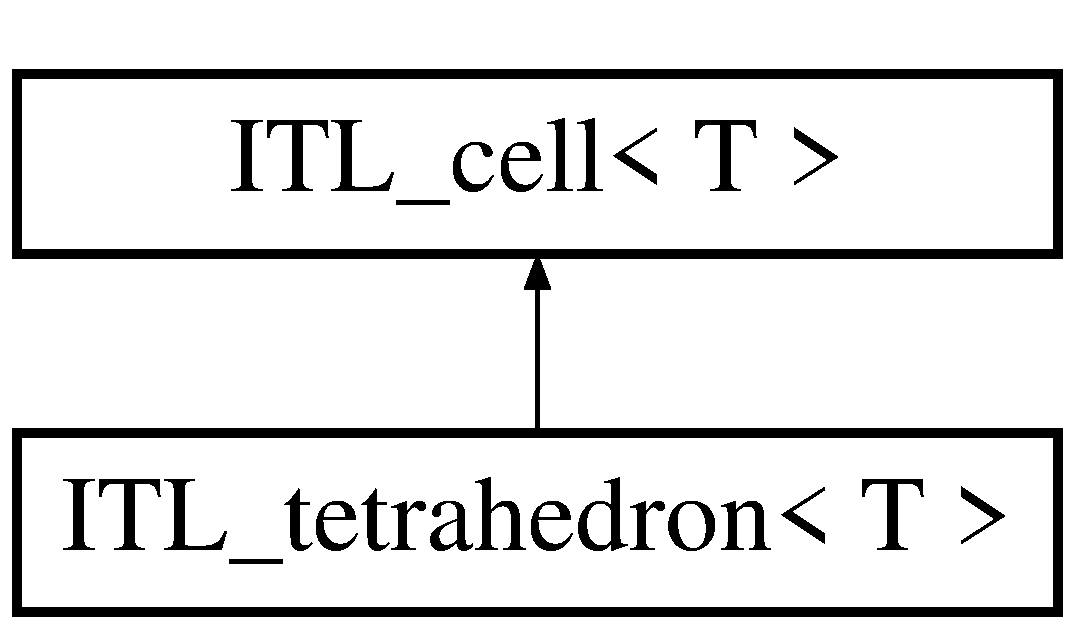
\includegraphics[height=2cm]{classITL__cell}
\end{center}
\end{figure}


\subsection{Detailed Description}
\subsubsection*{template$<$class T$>$ class ITL\_\-cell$<$ T $>$}

Cell class representing a unit of an unstructured grid. Created on: Apr 28, 2011 \begin{DoxyAuthor}{Author}
Abon 

Teng-\/Yok 
\end{DoxyAuthor}


Definition at line 12 of file ITL\_\-cell.h.



The documentation for this class was generated from the following file:\begin{DoxyCompactItemize}
\item 
/home/abon/Code/workspace\_\-unix/ITL\_\-repo/include/\hyperlink{ITL__cell_8h}{ITL\_\-cell.h}\end{DoxyCompactItemize}

\hypertarget{classITL__datastore}{
\section{ITL\_\-datastore$<$ T $>$ Class Template Reference}
\label{classITL__datastore}\index{ITL\_\-datastore@{ITL\_\-datastore}}
}


The container class for data.  




{\ttfamily \#include $<$ITL\_\-datastore.h$>$}

\subsection*{Public Member Functions}
\begin{DoxyCompactItemize}
\item 
\hyperlink{classITL__datastore_a1da115b3d395ac0482d2b0c980a2384f}{ITL\_\-datastore} ()
\begin{DoxyCompactList}\small\item\em Default Constructor. \item\end{DoxyCompactList}\item 
\hyperlink{classITL__datastore_a3beff9f7ee4e7ce2a65cc3bce3418b99}{ITL\_\-datastore} (T $\ast$\hyperlink{MainIT__regvector_8cpp_a783b2b1c03f80ec0d3ed965238d6bd65}{data})
\begin{DoxyCompactList}\small\item\em Constructor. \item\end{DoxyCompactList}\item 
\hyperlink{classITL__datastore_a017cff7441532e53a2a0897cc8790e3a}{ITL\_\-datastore} (int nData)
\begin{DoxyCompactList}\small\item\em Constructor. \item\end{DoxyCompactList}\item 
virtual bool \hyperlink{classITL__datastore_a43b1843d9ccedc71295116de3d31edb0}{hasData} ()
\begin{DoxyCompactList}\small\item\em Boolean function that returns TRUE if datastore contains data. \item\end{DoxyCompactList}\item 
virtual T $\ast$ \hyperlink{classITL__datastore_ac5d73b1499462140fafa2ca90634c721}{getData} ()
\begin{DoxyCompactList}\small\item\em Data accessor function. \item\end{DoxyCompactList}\item 
\hyperlink{classITL__datastore_a4691b58e9218237b709195d8f2a811eb}{$\sim$ITL\_\-datastore} ()
\begin{DoxyCompactList}\small\item\em Destructor. \item\end{DoxyCompactList}\end{DoxyCompactItemize}
\subsection*{Public Attributes}
\begin{DoxyCompactItemize}
\item 
FILE $\ast$ \hyperlink{classITL__datastore_a63d8cfcd308a6dd6763bd784c3870197}{datafile}
\begin{DoxyCompactList}\small\item\em Pointer to data file. \item\end{DoxyCompactList}\item 
int \hyperlink{classITL__datastore_aceb858e3255e686bc8567e4f203adc88}{nel}
\begin{DoxyCompactList}\small\item\em Total number of elements in the 1D array. \item\end{DoxyCompactList}\item 
T $\ast$ \hyperlink{classITL__datastore_a63e6e00d86fa6f227686e0612518e26e}{array}
\begin{DoxyCompactList}\small\item\em Pointer to the 1D array containing data elements. \item\end{DoxyCompactList}\end{DoxyCompactItemize}


\subsection{Detailed Description}
\subsubsection*{template$<$class T$>$ class ITL\_\-datastore$<$ T $>$}

The container class for data. This template class is the container for the raw data for a field. This class does not have any information regarding indexing and spatial arrangement of the data. Created on: Nov 18, 2010. \begin{DoxyAuthor}{Authors}
Abon 
\end{DoxyAuthor}
\begin{DoxyAuthor}{Author}
Teng-\/Yok 
\end{DoxyAuthor}
\begin{DoxySeeAlso}{See also}
\hyperlink{classITL__grid}{ITL\_\-grid} 
\end{DoxySeeAlso}


Definition at line 17 of file ITL\_\-datastore.h.



\subsection{Constructor \& Destructor Documentation}
\hypertarget{classITL__datastore_a1da115b3d395ac0482d2b0c980a2384f}{
\index{ITL\_\-datastore@{ITL\_\-datastore}!ITL\_\-datastore@{ITL\_\-datastore}}
\index{ITL\_\-datastore@{ITL\_\-datastore}!ITL_datastore@{ITL\_\-datastore}}
\subsubsection[{ITL\_\-datastore}]{\setlength{\rightskip}{0pt plus 5cm}template$<$class T$>$ {\bf ITL\_\-datastore}$<$ T $>$::{\bf ITL\_\-datastore} ()\hspace{0.3cm}{\ttfamily  \mbox{[}inline\mbox{]}}}}
\label{classITL__datastore_a1da115b3d395ac0482d2b0c980a2384f}


Default Constructor. 



Definition at line 30 of file ITL\_\-datastore.h.

\hypertarget{classITL__datastore_a3beff9f7ee4e7ce2a65cc3bce3418b99}{
\index{ITL\_\-datastore@{ITL\_\-datastore}!ITL\_\-datastore@{ITL\_\-datastore}}
\index{ITL\_\-datastore@{ITL\_\-datastore}!ITL_datastore@{ITL\_\-datastore}}
\subsubsection[{ITL\_\-datastore}]{\setlength{\rightskip}{0pt plus 5cm}template$<$class T$>$ {\bf ITL\_\-datastore}$<$ T $>$::{\bf ITL\_\-datastore} (T $\ast$ {\em data})\hspace{0.3cm}{\ttfamily  \mbox{[}inline\mbox{]}}}}
\label{classITL__datastore_a3beff9f7ee4e7ce2a65cc3bce3418b99}


Constructor. 


\begin{DoxyParams}{Parameters}
\item[{\em data}]pointer to template array conaining data. \end{DoxyParams}


Definition at line 41 of file ITL\_\-datastore.h.

\hypertarget{classITL__datastore_a017cff7441532e53a2a0897cc8790e3a}{
\index{ITL\_\-datastore@{ITL\_\-datastore}!ITL\_\-datastore@{ITL\_\-datastore}}
\index{ITL\_\-datastore@{ITL\_\-datastore}!ITL_datastore@{ITL\_\-datastore}}
\subsubsection[{ITL\_\-datastore}]{\setlength{\rightskip}{0pt plus 5cm}template$<$class T$>$ {\bf ITL\_\-datastore}$<$ T $>$::{\bf ITL\_\-datastore} (int {\em nData})\hspace{0.3cm}{\ttfamily  \mbox{[}inline\mbox{]}}}}
\label{classITL__datastore_a017cff7441532e53a2a0897cc8790e3a}


Constructor. 


\begin{DoxyParams}{Parameters}
\item[{\em nData}]Number of data elements. This constructor allocates memory for data. \end{DoxyParams}


Definition at line 53 of file ITL\_\-datastore.h.

\hypertarget{classITL__datastore_a4691b58e9218237b709195d8f2a811eb}{
\index{ITL\_\-datastore@{ITL\_\-datastore}!$\sim$ITL\_\-datastore@{$\sim$ITL\_\-datastore}}
\index{$\sim$ITL\_\-datastore@{$\sim$ITL\_\-datastore}!ITL_datastore@{ITL\_\-datastore}}
\subsubsection[{$\sim$ITL\_\-datastore}]{\setlength{\rightskip}{0pt plus 5cm}template$<$class T$>$ {\bf ITL\_\-datastore}$<$ T $>$::$\sim${\bf ITL\_\-datastore} ()\hspace{0.3cm}{\ttfamily  \mbox{[}inline\mbox{]}}}}
\label{classITL__datastore_a4691b58e9218237b709195d8f2a811eb}


Destructor. 



Definition at line 81 of file ITL\_\-datastore.h.



\subsection{Member Function Documentation}
\hypertarget{classITL__datastore_ac5d73b1499462140fafa2ca90634c721}{
\index{ITL\_\-datastore@{ITL\_\-datastore}!getData@{getData}}
\index{getData@{getData}!ITL_datastore@{ITL\_\-datastore}}
\subsubsection[{getData}]{\setlength{\rightskip}{0pt plus 5cm}template$<$class T$>$ virtual T$\ast$ {\bf ITL\_\-datastore}$<$ T $>$::getData ()\hspace{0.3cm}{\ttfamily  \mbox{[}inline, virtual\mbox{]}}}}
\label{classITL__datastore_ac5d73b1499462140fafa2ca90634c721}


Data accessor function. 

\begin{DoxyReturn}{Returns}
Pointer to data. 
\end{DoxyReturn}


Definition at line 73 of file ITL\_\-datastore.h.

\hypertarget{classITL__datastore_a43b1843d9ccedc71295116de3d31edb0}{
\index{ITL\_\-datastore@{ITL\_\-datastore}!hasData@{hasData}}
\index{hasData@{hasData}!ITL_datastore@{ITL\_\-datastore}}
\subsubsection[{hasData}]{\setlength{\rightskip}{0pt plus 5cm}template$<$class T$>$ virtual bool {\bf ITL\_\-datastore}$<$ T $>$::hasData ()\hspace{0.3cm}{\ttfamily  \mbox{[}inline, virtual\mbox{]}}}}
\label{classITL__datastore_a43b1843d9ccedc71295116de3d31edb0}


Boolean function that returns TRUE if datastore contains data. 

\begin{DoxyReturn}{Returns}
Boolean flag. 
\end{DoxyReturn}


Definition at line 64 of file ITL\_\-datastore.h.



\subsection{Member Data Documentation}
\hypertarget{classITL__datastore_a63e6e00d86fa6f227686e0612518e26e}{
\index{ITL\_\-datastore@{ITL\_\-datastore}!array@{array}}
\index{array@{array}!ITL_datastore@{ITL\_\-datastore}}
\subsubsection[{array}]{\setlength{\rightskip}{0pt plus 5cm}template$<$class T$>$ T$\ast$ {\bf ITL\_\-datastore}$<$ T $>$::{\bf array}}}
\label{classITL__datastore_a63e6e00d86fa6f227686e0612518e26e}


Pointer to the 1D array containing data elements. 



Definition at line 23 of file ITL\_\-datastore.h.

\hypertarget{classITL__datastore_a63d8cfcd308a6dd6763bd784c3870197}{
\index{ITL\_\-datastore@{ITL\_\-datastore}!datafile@{datafile}}
\index{datafile@{datafile}!ITL_datastore@{ITL\_\-datastore}}
\subsubsection[{datafile}]{\setlength{\rightskip}{0pt plus 5cm}template$<$class T$>$ FILE$\ast$ {\bf ITL\_\-datastore}$<$ T $>$::{\bf datafile}}}
\label{classITL__datastore_a63d8cfcd308a6dd6763bd784c3870197}


Pointer to data file. 

Required if data has to be read directly from file. 

Definition at line 21 of file ITL\_\-datastore.h.

\hypertarget{classITL__datastore_aceb858e3255e686bc8567e4f203adc88}{
\index{ITL\_\-datastore@{ITL\_\-datastore}!nel@{nel}}
\index{nel@{nel}!ITL_datastore@{ITL\_\-datastore}}
\subsubsection[{nel}]{\setlength{\rightskip}{0pt plus 5cm}template$<$class T$>$ int {\bf ITL\_\-datastore}$<$ T $>$::{\bf nel}}}
\label{classITL__datastore_aceb858e3255e686bc8567e4f203adc88}


Total number of elements in the 1D array. 



Definition at line 22 of file ITL\_\-datastore.h.



The documentation for this class was generated from the following file:\begin{DoxyCompactItemize}
\item 
/home/abon/Code/workspace\_\-unix/ITL\_\-repo/include/\hyperlink{ITL__datastore_8h}{ITL\_\-datastore.h}\end{DoxyCompactItemize}

\hypertarget{classITL__entropy}{
\section{ITL\_\-entropy$<$ T $>$ Class Template Reference}
\label{classITL__entropy}\index{ITL\_\-entropy@{ITL\_\-entropy}}
}


Entropy computation class.  




{\ttfamily \#include $<$ITL\_\-entropy.h$>$}

\subsection*{Public Member Functions}
\begin{DoxyCompactItemize}
\item 
\hyperlink{classITL__entropy_a1f446a47b389fe894139cefd9843c0dc}{ITL\_\-entropy} (\hyperlink{classITL__field__regular}{ITL\_\-field\_\-regular}$<$ T $>$ $\ast$f)
\begin{DoxyCompactList}\small\item\em Default Constructor. \item\end{DoxyCompactList}\item 
void \hyperlink{classITL__entropy_a39aa28b0d3d0964bee919d23fe3768d7}{computeHistogramBinField} (int nBins)
\begin{DoxyCompactList}\small\item\em Histogram bin assignment function. \item\end{DoxyCompactList}\item 
void \hyperlink{classITL__entropy_a4ad3dd3d26770b6e651d936e2914ed2f}{computeEntropyOfField} (int nBins)
\begin{DoxyCompactList}\small\item\em Entropy computation function. \item\end{DoxyCompactList}\item 
void \hyperlink{classITL__entropy_aedf49a83fa884a6a4c191a0ddba518dd}{computeEntropySinglePoint} (int x, int y, int z, int nNeighbors, int nBins, int entropyFieldIndex)
\begin{DoxyCompactList}\small\item\em Entropy computation function. \item\end{DoxyCompactList}\item 
float \hyperlink{classITL__entropy_a2c5655a1f68d7942dc98d98fe330660a}{computeEntropy} (int $\ast$binIds, int nels, int nbins)
\begin{DoxyCompactList}\small\item\em Entropy computation function. \item\end{DoxyCompactList}\item 
float \hyperlink{classITL__entropy_ad953a52d2910a04ead0fc40e5af10590}{getEntropy} ()
\begin{DoxyCompactList}\small\item\em Entropy accessor function. \item\end{DoxyCompactList}\item 
\hyperlink{classITL__field__regular}{ITL\_\-field\_\-regular}$<$ float $>$ $\ast$ \hyperlink{classITL__entropy_a640b8cb03be2ce05dcdb5ffa683dd9c9}{getEntropyField} ()
\begin{DoxyCompactList}\small\item\em Entropy field accessor function. \item\end{DoxyCompactList}\end{DoxyCompactItemize}
\subsection*{Public Attributes}
\begin{DoxyCompactItemize}
\item 
\hyperlink{classITL__field__regular}{ITL\_\-field\_\-regular}$<$ T $>$ $\ast$ \hyperlink{classITL__entropy_aa37a62d817f8cd335b63d4d9a9239e10}{dataField}
\item 
\hyperlink{classITL__field__regular}{ITL\_\-field\_\-regular}$<$ int $>$ $\ast$ \hyperlink{classITL__entropy_ae719783c7a6ae4481b711a1caf9e3ded}{binData}
\begin{DoxyCompactList}\small\item\em A scalar field containing histogram bins corresponding to field points. \item\end{DoxyCompactList}\item 
\hyperlink{classITL__field__regular}{ITL\_\-field\_\-regular}$<$ float $>$ $\ast$ \hyperlink{classITL__entropy_ac9940978878a0f624d94ada66fc1bfd5}{entropyField}
\item 
float \hyperlink{classITL__entropy_afea389e705dfeb2a6924a84e9055777d}{entropy}
\begin{DoxyCompactList}\small\item\em Value of computed entropy at a specified point in the field. \item\end{DoxyCompactList}\item 
float $\ast$ \hyperlink{classITL__entropy_abd080665e882ac3a2e56fd23ec104114}{probarray}
\begin{DoxyCompactList}\small\item\em Probability array used in emtropy computation. \item\end{DoxyCompactList}\end{DoxyCompactItemize}


\subsection{Detailed Description}
\subsubsection*{template$<$class T$>$ class ITL\_\-entropy$<$ T $>$}

Entropy computation class. Created on: Nov 19, 2010. \begin{DoxyAuthor}{Author}
Abon 

Teng-\/Yok 
\end{DoxyAuthor}


Definition at line 15 of file ITL\_\-entropy.h.



\subsection{Constructor \& Destructor Documentation}
\hypertarget{classITL__entropy_a1f446a47b389fe894139cefd9843c0dc}{
\index{ITL\_\-entropy@{ITL\_\-entropy}!ITL\_\-entropy@{ITL\_\-entropy}}
\index{ITL\_\-entropy@{ITL\_\-entropy}!ITL_entropy@{ITL\_\-entropy}}
\subsubsection[{ITL\_\-entropy}]{\setlength{\rightskip}{0pt plus 5cm}template$<$class T $>$ {\bf ITL\_\-entropy}$<$ T $>$::{\bf ITL\_\-entropy} ({\bf ITL\_\-field\_\-regular}$<$ T $>$ $\ast$ {\em f})\hspace{0.3cm}{\ttfamily  \mbox{[}inline\mbox{]}}}}
\label{classITL__entropy_a1f446a47b389fe894139cefd9843c0dc}


Default Constructor. 



Definition at line 27 of file ITL\_\-entropy.h.



\subsection{Member Function Documentation}
\hypertarget{classITL__entropy_a2c5655a1f68d7942dc98d98fe330660a}{
\index{ITL\_\-entropy@{ITL\_\-entropy}!computeEntropy@{computeEntropy}}
\index{computeEntropy@{computeEntropy}!ITL_entropy@{ITL\_\-entropy}}
\subsubsection[{computeEntropy}]{\setlength{\rightskip}{0pt plus 5cm}template$<$class T $>$ float {\bf ITL\_\-entropy}$<$ T $>$::computeEntropy (int $\ast$ {\em binIds}, \/  int {\em nels}, \/  int {\em nbins})\hspace{0.3cm}{\ttfamily  \mbox{[}inline\mbox{]}}}}
\label{classITL__entropy_a2c5655a1f68d7942dc98d98fe330660a}


Entropy computation function. 


\begin{DoxyParams}{Parameters}
\item[{\em binIds}]Pointer to array containing histogram bin assignments of the points in the neighborhood. \item[{\em nels}]Number of points in the neighborhood. Same as the length of bin array. \item[{\em nbins}]Number of bins used in histogram computation. \end{DoxyParams}


Definition at line 198 of file ITL\_\-entropy.h.

\hypertarget{classITL__entropy_a4ad3dd3d26770b6e651d936e2914ed2f}{
\index{ITL\_\-entropy@{ITL\_\-entropy}!computeEntropyOfField@{computeEntropyOfField}}
\index{computeEntropyOfField@{computeEntropyOfField}!ITL_entropy@{ITL\_\-entropy}}
\subsubsection[{computeEntropyOfField}]{\setlength{\rightskip}{0pt plus 5cm}template$<$class T $>$ void {\bf ITL\_\-entropy}$<$ T $>$::computeEntropyOfField (int {\em nBins})\hspace{0.3cm}{\ttfamily  \mbox{[}inline\mbox{]}}}}
\label{classITL__entropy_a4ad3dd3d26770b6e651d936e2914ed2f}


Entropy computation function. 

Creates a scalar field that contains entropy at each grid vertex. 
\begin{DoxyParams}{Parameters}
\item[{\em nBins}]Number of bins used in histogram computation. \end{DoxyParams}


Definition at line 96 of file ITL\_\-entropy.h.

\hypertarget{classITL__entropy_aedf49a83fa884a6a4c191a0ddba518dd}{
\index{ITL\_\-entropy@{ITL\_\-entropy}!computeEntropySinglePoint@{computeEntropySinglePoint}}
\index{computeEntropySinglePoint@{computeEntropySinglePoint}!ITL_entropy@{ITL\_\-entropy}}
\subsubsection[{computeEntropySinglePoint}]{\setlength{\rightskip}{0pt plus 5cm}template$<$class T $>$ void {\bf ITL\_\-entropy}$<$ T $>$::computeEntropySinglePoint (int {\em x}, \/  int {\em y}, \/  int {\em z}, \/  int {\em nNeighbors}, \/  int {\em nBins}, \/  int {\em entropyFieldIndex})\hspace{0.3cm}{\ttfamily  \mbox{[}inline\mbox{]}}}}
\label{classITL__entropy_aedf49a83fa884a6a4c191a0ddba518dd}


Entropy computation function. 

Computes entropy at a spatial point in the field. 
\begin{DoxyParams}{Parameters}
\item[{\em x}]x-\/coordinate of the spatial point. \item[{\em y}]y-\/coordinate of the spatial point. \item[{\em z}]z-\/coordinate of the spatial point. \item[{\em nNeighbors}]total number of neighbors in the neighborhood (including self). \item[{\em nBins}]Number of bins to use in histogram computation. \item[{\em entropyFieldIndex}]1D index to the entopy field. \end{DoxyParams}


Definition at line 141 of file ITL\_\-entropy.h.

\hypertarget{classITL__entropy_a39aa28b0d3d0964bee919d23fe3768d7}{
\index{ITL\_\-entropy@{ITL\_\-entropy}!computeHistogramBinField@{computeHistogramBinField}}
\index{computeHistogramBinField@{computeHistogramBinField}!ITL_entropy@{ITL\_\-entropy}}
\subsubsection[{computeHistogramBinField}]{\setlength{\rightskip}{0pt plus 5cm}template$<$class T $>$ void {\bf ITL\_\-entropy}$<$ T $>$::computeHistogramBinField (int {\em nBins})\hspace{0.3cm}{\ttfamily  \mbox{[}inline\mbox{]}}}}
\label{classITL__entropy_a39aa28b0d3d0964bee919d23fe3768d7}


Histogram bin assignment function. 

Creates a scalar field of histogram at each grid vertex. 
\begin{DoxyParams}{Parameters}
\item[{\em nBins}]Number of bins to use in histogram computation. \end{DoxyParams}


Definition at line 39 of file ITL\_\-entropy.h.

\hypertarget{classITL__entropy_ad953a52d2910a04ead0fc40e5af10590}{
\index{ITL\_\-entropy@{ITL\_\-entropy}!getEntropy@{getEntropy}}
\index{getEntropy@{getEntropy}!ITL_entropy@{ITL\_\-entropy}}
\subsubsection[{getEntropy}]{\setlength{\rightskip}{0pt plus 5cm}template$<$class T $>$ float {\bf ITL\_\-entropy}$<$ T $>$::getEntropy ()}}
\label{classITL__entropy_ad953a52d2910a04ead0fc40e5af10590}


Entropy accessor function. 

\begin{DoxyReturn}{Returns}
computed entropy. 
\end{DoxyReturn}
\hypertarget{classITL__entropy_a640b8cb03be2ce05dcdb5ffa683dd9c9}{
\index{ITL\_\-entropy@{ITL\_\-entropy}!getEntropyField@{getEntropyField}}
\index{getEntropyField@{getEntropyField}!ITL_entropy@{ITL\_\-entropy}}
\subsubsection[{getEntropyField}]{\setlength{\rightskip}{0pt plus 5cm}template$<$class T $>$ {\bf ITL\_\-field\_\-regular}$<$float$>$$\ast$ {\bf ITL\_\-entropy}$<$ T $>$::getEntropyField ()\hspace{0.3cm}{\ttfamily  \mbox{[}inline\mbox{]}}}}
\label{classITL__entropy_a640b8cb03be2ce05dcdb5ffa683dd9c9}


Entropy field accessor function. 

Returns computed entropy field. \begin{DoxyReturn}{Returns}
pointer to entropy field. 
\end{DoxyReturn}


Definition at line 238 of file ITL\_\-entropy.h.



\subsection{Member Data Documentation}
\hypertarget{classITL__entropy_ae719783c7a6ae4481b711a1caf9e3ded}{
\index{ITL\_\-entropy@{ITL\_\-entropy}!binData@{binData}}
\index{binData@{binData}!ITL_entropy@{ITL\_\-entropy}}
\subsubsection[{binData}]{\setlength{\rightskip}{0pt plus 5cm}template$<$class T $>$ {\bf ITL\_\-field\_\-regular}$<$int$>$$\ast$ {\bf ITL\_\-entropy}$<$ T $>$::{\bf binData}}}
\label{classITL__entropy_ae719783c7a6ae4481b711a1caf9e3ded}


A scalar field containing histogram bins corresponding to field points. 



Definition at line 17 of file ITL\_\-entropy.h.

\hypertarget{classITL__entropy_aa37a62d817f8cd335b63d4d9a9239e10}{
\index{ITL\_\-entropy@{ITL\_\-entropy}!dataField@{dataField}}
\index{dataField@{dataField}!ITL_entropy@{ITL\_\-entropy}}
\subsubsection[{dataField}]{\setlength{\rightskip}{0pt plus 5cm}template$<$class T $>$ {\bf ITL\_\-field\_\-regular}$<$T$>$$\ast$ {\bf ITL\_\-entropy}$<$ T $>$::{\bf dataField}}}
\label{classITL__entropy_aa37a62d817f8cd335b63d4d9a9239e10}


Definition at line 16 of file ITL\_\-entropy.h.

\hypertarget{classITL__entropy_afea389e705dfeb2a6924a84e9055777d}{
\index{ITL\_\-entropy@{ITL\_\-entropy}!entropy@{entropy}}
\index{entropy@{entropy}!ITL_entropy@{ITL\_\-entropy}}
\subsubsection[{entropy}]{\setlength{\rightskip}{0pt plus 5cm}template$<$class T $>$ float {\bf ITL\_\-entropy}$<$ T $>$::{\bf entropy}}}
\label{classITL__entropy_afea389e705dfeb2a6924a84e9055777d}


Value of computed entropy at a specified point in the field. 



Definition at line 20 of file ITL\_\-entropy.h.

\hypertarget{classITL__entropy_ac9940978878a0f624d94ada66fc1bfd5}{
\index{ITL\_\-entropy@{ITL\_\-entropy}!entropyField@{entropyField}}
\index{entropyField@{entropyField}!ITL_entropy@{ITL\_\-entropy}}
\subsubsection[{entropyField}]{\setlength{\rightskip}{0pt plus 5cm}template$<$class T $>$ {\bf ITL\_\-field\_\-regular}$<$float$>$$\ast$ {\bf ITL\_\-entropy}$<$ T $>$::{\bf entropyField}}}
\label{classITL__entropy_ac9940978878a0f624d94ada66fc1bfd5}


Definition at line 18 of file ITL\_\-entropy.h.

\hypertarget{classITL__entropy_abd080665e882ac3a2e56fd23ec104114}{
\index{ITL\_\-entropy@{ITL\_\-entropy}!probarray@{probarray}}
\index{probarray@{probarray}!ITL_entropy@{ITL\_\-entropy}}
\subsubsection[{probarray}]{\setlength{\rightskip}{0pt plus 5cm}template$<$class T $>$ float$\ast$ {\bf ITL\_\-entropy}$<$ T $>$::{\bf probarray}}}
\label{classITL__entropy_abd080665e882ac3a2e56fd23ec104114}


Probability array used in emtropy computation. 



Definition at line 21 of file ITL\_\-entropy.h.



The documentation for this class was generated from the following file:\begin{DoxyCompactItemize}
\item 
/home/abon/Code/workspace\_\-unix/ITL\_\-repo/include/\hyperlink{ITL__entropy_8h}{ITL\_\-entropy.h}\end{DoxyCompactItemize}

\hypertarget{classITL__entropycore}{
\section{ITL\_\-entropycore Class Reference}
\label{classITL__entropycore}\index{ITL\_\-entropycore@{ITL\_\-entropycore}}
}


Entropy computation core class.  




{\ttfamily \#include $<$ITL\_\-entropycore.h$>$}

\subsection*{Static Public Member Functions}
\begin{DoxyCompactItemize}
\item 
static float \hyperlink{classITL__entropycore_afd605a02922df607f43d0b1ec3248e7d}{computeEntropy\_\-HistogramBased} (int $\ast$binIds, int nPoint, int \hyperlink{MainIT__regvector_8cpp_a7f13753d4707f6bc8f71d8bdacedefb3}{nBin}, bool toNormalize)
\begin{DoxyCompactList}\small\item\em Histogram based entropy computation function. \item\end{DoxyCompactList}\item 
static float \hyperlink{classITL__entropycore_a44a6bc62c22f739825a4b7dcf10ab43a}{computeEntropy\_\-KDEBased} (float $\ast$\hyperlink{MainIT__regvector_8cpp_a783b2b1c03f80ec0d3ed965238d6bd65}{data}, int nPoint, float h, bool toNormalize)
\begin{DoxyCompactList}\small\item\em KDE based entropy computation function. \item\end{DoxyCompactList}\item 
static float \hyperlink{classITL__entropycore_a5802a6a76dba25a5afa2b232eb69b9c2}{evaluateKernel} (float x, float mu, float var)
\begin{DoxyCompactList}\small\item\em Gaussian kernel evaluation function. \item\end{DoxyCompactList}\end{DoxyCompactItemize}


\subsection{Detailed Description}
Entropy computation core class. Created on: May 03, 2011. \begin{DoxyAuthor}{Author}
Abon 

Teng-\/Yok 
\end{DoxyAuthor}


Definition at line 14 of file ITL\_\-entropycore.h.



\subsection{Member Function Documentation}
\hypertarget{classITL__entropycore_afd605a02922df607f43d0b1ec3248e7d}{
\index{ITL\_\-entropycore@{ITL\_\-entropycore}!computeEntropy\_\-HistogramBased@{computeEntropy\_\-HistogramBased}}
\index{computeEntropy\_\-HistogramBased@{computeEntropy\_\-HistogramBased}!ITL_entropycore@{ITL\_\-entropycore}}
\subsubsection[{computeEntropy\_\-HistogramBased}]{\setlength{\rightskip}{0pt plus 5cm}float ITL\_\-entropycore::computeEntropy\_\-HistogramBased (int $\ast$ {\em binIds}, \/  int {\em nPoint}, \/  int {\em nBin}, \/  bool {\em toNormalize})\hspace{0.3cm}{\ttfamily  \mbox{[}static\mbox{]}}}}
\label{classITL__entropycore_afd605a02922df607f43d0b1ec3248e7d}


Histogram based entropy computation function. 


\begin{DoxyParams}{Parameters}
\item[{\em binIds}]Pointer to array containing histogram bin assignments of the points. \item[{\em nPoint}]Number of points. Same as the length of bin array. \item[{\em nBin}]Number of bins used in histogram computation. \end{DoxyParams}


Definition at line 3 of file ITL\_\-entropycore.cpp.

\hypertarget{classITL__entropycore_a44a6bc62c22f739825a4b7dcf10ab43a}{
\index{ITL\_\-entropycore@{ITL\_\-entropycore}!computeEntropy\_\-KDEBased@{computeEntropy\_\-KDEBased}}
\index{computeEntropy\_\-KDEBased@{computeEntropy\_\-KDEBased}!ITL_entropycore@{ITL\_\-entropycore}}
\subsubsection[{computeEntropy\_\-KDEBased}]{\setlength{\rightskip}{0pt plus 5cm}float ITL\_\-entropycore::computeEntropy\_\-KDEBased (float $\ast$ {\em data}, \/  int {\em nPoint}, \/  float {\em h}, \/  bool {\em toNormalize})\hspace{0.3cm}{\ttfamily  \mbox{[}static\mbox{]}}}}
\label{classITL__entropycore_a44a6bc62c22f739825a4b7dcf10ab43a}


KDE based entropy computation function. 


\begin{DoxyParams}{Parameters}
\item[{\em data}]Pointer to data array. \item[{\em nPoint}]Number of points to be sampled. Equivalent to nBin. \item[{\em h}]Kernel Bandwidth (Put 0 to allow the software decide the bandwidth) \item[{\em toNormalize}]TRUE indicates the computed entropy will be normalized. \end{DoxyParams}


Definition at line 39 of file ITL\_\-entropycore.cpp.

\hypertarget{classITL__entropycore_a5802a6a76dba25a5afa2b232eb69b9c2}{
\index{ITL\_\-entropycore@{ITL\_\-entropycore}!evaluateKernel@{evaluateKernel}}
\index{evaluateKernel@{evaluateKernel}!ITL_entropycore@{ITL\_\-entropycore}}
\subsubsection[{evaluateKernel}]{\setlength{\rightskip}{0pt plus 5cm}float ITL\_\-entropycore::evaluateKernel (float {\em x}, \/  float {\em mu}, \/  float {\em var})\hspace{0.3cm}{\ttfamily  \mbox{[}static\mbox{]}}}}
\label{classITL__entropycore_a5802a6a76dba25a5afa2b232eb69b9c2}


Gaussian kernel evaluation function. 

Returns N( (x-\/mu)/sigma $|$0, 1 ) for some sample x.. 
\begin{DoxyParams}{Parameters}
\item[{\em mu}]Mean of the point set  var Variance of the point set \end{DoxyParams}


Definition at line 88 of file ITL\_\-entropycore.cpp.



The documentation for this class was generated from the following files:\begin{DoxyCompactItemize}
\item 
/home/abon/Code/workspace\_\-unix/ITL\_\-repo/include/\hyperlink{ITL__entropycore_8h}{ITL\_\-entropycore.h}\item 
/home/abon/Code/workspace\_\-unix/ITL\_\-repo/src/\hyperlink{ITL__entropycore_8cpp}{ITL\_\-entropycore.cpp}\end{DoxyCompactItemize}

\hypertarget{classITL__field}{
\section{ITL\_\-field$<$ T $>$ Class Template Reference}
\label{classITL__field}\index{ITL\_\-field@{ITL\_\-field}}
}


Field base class.  




{\ttfamily \#include $<$ITL\_\-field.h$>$}

Inheritance diagram for ITL\_\-field$<$ T $>$:\begin{figure}[H]
\begin{center}
\leavevmode
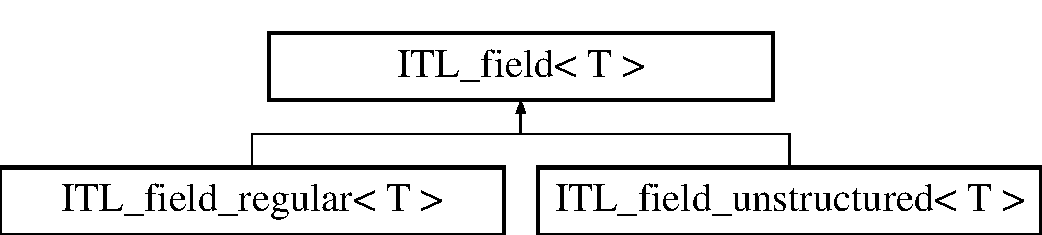
\includegraphics[height=2cm]{classITL__field}
\end{center}
\end{figure}
\subsection*{Public Member Functions}
\begin{DoxyCompactItemize}
\item 
\hyperlink{classITL__field_acbb918b7ab99fe46d837465d16d4adab}{ITL\_\-field} ()
\begin{DoxyCompactList}\small\item\em Default constructor. \item\end{DoxyCompactList}\item 
virtual void \hyperlink{classITL__field_a134f7a48123be7d3fbfcb52b4bcbb5c8}{setBounds} ()
\begin{DoxyCompactList}\small\item\em Pure virtual function. \item\end{DoxyCompactList}\item 
virtual void \hyperlink{classITL__field_a7bf82ed82a338d34985a6758307c8ece}{setBounds} (float $\ast$, float $\ast$)
\begin{DoxyCompactList}\small\item\em Pure virtual function for setting the bounds of a field with no ghost layers. \item\end{DoxyCompactList}\item 
virtual void \hyperlink{classITL__field_ab27b49b81f3a7a2a614eaca91cd8eb8c}{setBounds} (float $\ast$, float $\ast$, int $\ast$, int $\ast$, int)
\begin{DoxyCompactList}\small\item\em Pure virtual function for setting the bounds of a grid with ghost layers. \item\end{DoxyCompactList}\item 
virtual void \hyperlink{classITL__field_a5c7ecb94890c0dd7d730e881f530bbc2}{partitionField} (int $\ast$nblocks)
\begin{DoxyCompactList}\small\item\em Pure virtual function for regular partitioning of the field. \item\end{DoxyCompactList}\item 
virtual \hyperlink{classITL__field}{ITL\_\-field} $\ast$ \hyperlink{classITL__field_a7ca32e8dd6186974778ae4c8302ee922}{createSubField} (float $\ast$\hyperlink{MainIT__regvector_8cpp_abb1e2dad97264e859f3ee8af1341d68c}{low}, float $\ast$\hyperlink{MainIT__regvector_8cpp_a2012a18ba7a98e566c072356d03c4240}{high})
\begin{DoxyCompactList}\small\item\em Pure virtual function for creating a partition or subfield within the specified bounds. \item\end{DoxyCompactList}\item 
virtual T \hyperlink{classITL__field_a9a4b41fbeafd49afde45b608b5db2c09}{getDataAt} (int id)
\begin{DoxyCompactList}\small\item\em Data accessor function type 1. \item\end{DoxyCompactList}\item 
virtual T \hyperlink{classITL__field_a40f9224e8815388882c953b914c540ff}{getDataAt} (int x, int y, int z)
\begin{DoxyCompactList}\small\item\em Data accessor function type 2. \item\end{DoxyCompactList}\item 
virtual T $\ast$ \hyperlink{classITL__field_ab3254f696ccca1b4ea1aae248bea989c}{getDataBetween} (int $\ast$lowBoundary, int $\ast$highBoundary)
\begin{DoxyCompactList}\small\item\em Data accessor function type 3. \item\end{DoxyCompactList}\item 
virtual T $\ast$ \hyperlink{classITL__field_a983bd8b95e95bf758a73fafccea62a49}{getDataBetween} (float $\ast$lowBoundary, float $\ast$highBoundary)
\begin{DoxyCompactList}\small\item\em Data accessor function type 4. \item\end{DoxyCompactList}\item 
virtual T $\ast$ \hyperlink{classITL__field_afba4c040443d3f21d3f4af30a70292be}{getDataFull} ()
\begin{DoxyCompactList}\small\item\em Data accessor function type 5. \item\end{DoxyCompactList}\item 
virtual void \hyperlink{classITL__field_ae87ee8fef9c9b9dc6a782ccbfe3605e1}{setDataAt} (int id, T \hyperlink{MainIT__regvector_8cpp_a783b2b1c03f80ec0d3ed965238d6bd65}{data})
\begin{DoxyCompactList}\small\item\em Data mutator function type 1. \item\end{DoxyCompactList}\item 
virtual void \hyperlink{classITL__field_aeea532e25732eb1582a937409a98d05e}{setDataAt} (int x, int y, int z, T \hyperlink{MainIT__regvector_8cpp_a783b2b1c03f80ec0d3ed965238d6bd65}{data})
\begin{DoxyCompactList}\small\item\em Data mutator function type 2. \item\end{DoxyCompactList}\item 
virtual void \hyperlink{classITL__field_a4bbd5103c5298ac87eaac25c759a98c7}{setDataBetween} (T $\ast$\hyperlink{MainIT__regvector_8cpp_a783b2b1c03f80ec0d3ed965238d6bd65}{data})
\begin{DoxyCompactList}\small\item\em Data mutator function type 3. \item\end{DoxyCompactList}\item 
virtual void \hyperlink{classITL__field_a0c32994fe56253d8c7111d670742afc1}{setDataFull} (T $\ast$\hyperlink{MainIT__regvector_8cpp_a783b2b1c03f80ec0d3ed965238d6bd65}{data})
\begin{DoxyCompactList}\small\item\em Data mutator function type 4. \item\end{DoxyCompactList}\item 
virtual \hyperlink{classITL__field_aa8ace26f8abdf8a2d7a94ea27f0e7a16}{$\sim$ITL\_\-field} ()
\begin{DoxyCompactList}\small\item\em Destructor. \item\end{DoxyCompactList}\end{DoxyCompactItemize}
\subsection*{Public Attributes}
\begin{DoxyCompactItemize}
\item 
\hyperlink{classITL__grid}{ITL\_\-grid}$<$ T $>$ $\ast$ \hyperlink{classITL__field_a6c1bd62b59c41067f23f70ee2dc8a25a}{grid}
\begin{DoxyCompactList}\small\item\em Grid associated to the field. \item\end{DoxyCompactList}\item 
\hyperlink{classITL__datastore}{ITL\_\-datastore}$<$ T $>$ $\ast$ \hyperlink{classITL__field_aab9c6cdf9f4a7f3cd338e92c1dad9931}{datastore}
\begin{DoxyCompactList}\small\item\em Data store associated to the field. \item\end{DoxyCompactList}\item 
\hyperlink{classITL__field}{ITL\_\-field}$<$ T $>$ $\ast$ \hyperlink{classITL__field_a1ade5ffd6676a8df656447ce8512c75e}{subfieldArray}
\begin{DoxyCompactList}\small\item\em An array of sub fields (also referred to as blocks). \item\end{DoxyCompactList}\item 
float $\ast$ \hyperlink{classITL__field_a705d31afd5f130e8d977a0b7aab68fec}{blockSize}
\begin{DoxyCompactList}\small\item\em Length of subfield along each dimension. \item\end{DoxyCompactList}\item 
int $\ast$ \hyperlink{classITL__field_ac5ed068558f49ef1a7113f576e4adfc6}{nPartition}
\begin{DoxyCompactList}\small\item\em Number of subfields along each dimension. \item\end{DoxyCompactList}\end{DoxyCompactItemize}


\subsection{Detailed Description}
\subsubsection*{template$<$class T$>$ class ITL\_\-field$<$ T $>$}

Field base class. A generic class for a field which is a generic container for static/time-\/varying scalar/vector data. Created on: Nov 17, 2010. \begin{DoxyAuthor}{Author}
Abon 

Teng-\/Yok 
\end{DoxyAuthor}
\begin{DoxySeeAlso}{See also}
\hyperlink{classITL__field}{ITL\_\-field} regular 
\end{DoxySeeAlso}


Definition at line 22 of file ITL\_\-field.h.



\subsection{Constructor \& Destructor Documentation}
\hypertarget{classITL__field_acbb918b7ab99fe46d837465d16d4adab}{
\index{ITL\_\-field@{ITL\_\-field}!ITL\_\-field@{ITL\_\-field}}
\index{ITL\_\-field@{ITL\_\-field}!ITL_field@{ITL\_\-field}}
\subsubsection[{ITL\_\-field}]{\setlength{\rightskip}{0pt plus 5cm}template$<$class T$>$ {\bf ITL\_\-field}$<$ T $>$::{\bf ITL\_\-field} ()\hspace{0.3cm}{\ttfamily  \mbox{[}inline\mbox{]}}}}
\label{classITL__field_acbb918b7ab99fe46d837465d16d4adab}


Default constructor. 



Definition at line 38 of file ITL\_\-field.h.

\hypertarget{classITL__field_aa8ace26f8abdf8a2d7a94ea27f0e7a16}{
\index{ITL\_\-field@{ITL\_\-field}!$\sim$ITL\_\-field@{$\sim$ITL\_\-field}}
\index{$\sim$ITL\_\-field@{$\sim$ITL\_\-field}!ITL_field@{ITL\_\-field}}
\subsubsection[{$\sim$ITL\_\-field}]{\setlength{\rightskip}{0pt plus 5cm}template$<$class T$>$ virtual {\bf ITL\_\-field}$<$ T $>$::$\sim${\bf ITL\_\-field} ()\hspace{0.3cm}{\ttfamily  \mbox{[}inline, virtual\mbox{]}}}}
\label{classITL__field_aa8ace26f8abdf8a2d7a94ea27f0e7a16}


Destructor. 



Definition at line 104 of file ITL\_\-field.h.



\subsection{Member Function Documentation}
\hypertarget{classITL__field_a7ca32e8dd6186974778ae4c8302ee922}{
\index{ITL\_\-field@{ITL\_\-field}!createSubField@{createSubField}}
\index{createSubField@{createSubField}!ITL_field@{ITL\_\-field}}
\subsubsection[{createSubField}]{\setlength{\rightskip}{0pt plus 5cm}template$<$class T$>$ virtual {\bf ITL\_\-field}$\ast$ {\bf ITL\_\-field}$<$ T $>$::createSubField (float $\ast$ {\em low}, \/  float $\ast$ {\em high})\hspace{0.3cm}{\ttfamily  \mbox{[}inline, virtual\mbox{]}}}}
\label{classITL__field_a7ca32e8dd6186974778ae4c8302ee922}


Pure virtual function for creating a partition or subfield within the specified bounds. 



Reimplemented in \hyperlink{classITL__field__regular_a600a5a99a3e696c3a6698f112933a90c}{ITL\_\-field\_\-regular$<$ T $>$}, \hyperlink{classITL__field__regular_a600a5a99a3e696c3a6698f112933a90c}{ITL\_\-field\_\-regular$<$ float $>$}, and \hyperlink{classITL__field__regular_a600a5a99a3e696c3a6698f112933a90c}{ITL\_\-field\_\-regular$<$ int $>$}.



Definition at line 62 of file ITL\_\-field.h.

\hypertarget{classITL__field_a40f9224e8815388882c953b914c540ff}{
\index{ITL\_\-field@{ITL\_\-field}!getDataAt@{getDataAt}}
\index{getDataAt@{getDataAt}!ITL_field@{ITL\_\-field}}
\subsubsection[{getDataAt}]{\setlength{\rightskip}{0pt plus 5cm}template$<$class T$>$ virtual T {\bf ITL\_\-field}$<$ T $>$::getDataAt (int {\em x}, \/  int {\em y}, \/  int {\em z})\hspace{0.3cm}{\ttfamily  \mbox{[}inline, virtual\mbox{]}}}}
\label{classITL__field_a40f9224e8815388882c953b914c540ff}


Data accessor function type 2. 



Reimplemented in \hyperlink{classITL__field__regular_ad05668c219a4632a3ceaca8409339103}{ITL\_\-field\_\-regular$<$ T $>$}, \hyperlink{classITL__field__regular_ad05668c219a4632a3ceaca8409339103}{ITL\_\-field\_\-regular$<$ float $>$}, and \hyperlink{classITL__field__regular_ad05668c219a4632a3ceaca8409339103}{ITL\_\-field\_\-regular$<$ int $>$}.



Definition at line 70 of file ITL\_\-field.h.

\hypertarget{classITL__field_a9a4b41fbeafd49afde45b608b5db2c09}{
\index{ITL\_\-field@{ITL\_\-field}!getDataAt@{getDataAt}}
\index{getDataAt@{getDataAt}!ITL_field@{ITL\_\-field}}
\subsubsection[{getDataAt}]{\setlength{\rightskip}{0pt plus 5cm}template$<$class T$>$ virtual T {\bf ITL\_\-field}$<$ T $>$::getDataAt (int {\em id})\hspace{0.3cm}{\ttfamily  \mbox{[}inline, virtual\mbox{]}}}}
\label{classITL__field_a9a4b41fbeafd49afde45b608b5db2c09}


Data accessor function type 1. 



Reimplemented in \hyperlink{classITL__field__regular_a78f814d7617aeb01c63def2f5f2e9caa}{ITL\_\-field\_\-regular$<$ T $>$}, \hyperlink{classITL__field__regular_a78f814d7617aeb01c63def2f5f2e9caa}{ITL\_\-field\_\-regular$<$ float $>$}, and \hyperlink{classITL__field__regular_a78f814d7617aeb01c63def2f5f2e9caa}{ITL\_\-field\_\-regular$<$ int $>$}.



Definition at line 66 of file ITL\_\-field.h.

\hypertarget{classITL__field_a983bd8b95e95bf758a73fafccea62a49}{
\index{ITL\_\-field@{ITL\_\-field}!getDataBetween@{getDataBetween}}
\index{getDataBetween@{getDataBetween}!ITL_field@{ITL\_\-field}}
\subsubsection[{getDataBetween}]{\setlength{\rightskip}{0pt plus 5cm}template$<$class T$>$ virtual T$\ast$ {\bf ITL\_\-field}$<$ T $>$::getDataBetween (float $\ast$ {\em lowBoundary}, \/  float $\ast$ {\em highBoundary})\hspace{0.3cm}{\ttfamily  \mbox{[}inline, virtual\mbox{]}}}}
\label{classITL__field_a983bd8b95e95bf758a73fafccea62a49}


Data accessor function type 4. 



Reimplemented in \hyperlink{classITL__field__regular_a13a2ec8f1e67b6a906d1799a58acf9bd}{ITL\_\-field\_\-regular$<$ T $>$}, \hyperlink{classITL__field__regular_a13a2ec8f1e67b6a906d1799a58acf9bd}{ITL\_\-field\_\-regular$<$ float $>$}, and \hyperlink{classITL__field__regular_a13a2ec8f1e67b6a906d1799a58acf9bd}{ITL\_\-field\_\-regular$<$ int $>$}.



Definition at line 78 of file ITL\_\-field.h.

\hypertarget{classITL__field_ab3254f696ccca1b4ea1aae248bea989c}{
\index{ITL\_\-field@{ITL\_\-field}!getDataBetween@{getDataBetween}}
\index{getDataBetween@{getDataBetween}!ITL_field@{ITL\_\-field}}
\subsubsection[{getDataBetween}]{\setlength{\rightskip}{0pt plus 5cm}template$<$class T$>$ virtual T$\ast$ {\bf ITL\_\-field}$<$ T $>$::getDataBetween (int $\ast$ {\em lowBoundary}, \/  int $\ast$ {\em highBoundary})\hspace{0.3cm}{\ttfamily  \mbox{[}inline, virtual\mbox{]}}}}
\label{classITL__field_ab3254f696ccca1b4ea1aae248bea989c}


Data accessor function type 3. 



Reimplemented in \hyperlink{classITL__field__regular_af0d8776246431db1f5069f2ce6eb4d2f}{ITL\_\-field\_\-regular$<$ T $>$}, \hyperlink{classITL__field__regular_af0d8776246431db1f5069f2ce6eb4d2f}{ITL\_\-field\_\-regular$<$ float $>$}, and \hyperlink{classITL__field__regular_af0d8776246431db1f5069f2ce6eb4d2f}{ITL\_\-field\_\-regular$<$ int $>$}.



Definition at line 74 of file ITL\_\-field.h.

\hypertarget{classITL__field_afba4c040443d3f21d3f4af30a70292be}{
\index{ITL\_\-field@{ITL\_\-field}!getDataFull@{getDataFull}}
\index{getDataFull@{getDataFull}!ITL_field@{ITL\_\-field}}
\subsubsection[{getDataFull}]{\setlength{\rightskip}{0pt plus 5cm}template$<$class T$>$ virtual T$\ast$ {\bf ITL\_\-field}$<$ T $>$::getDataFull ()\hspace{0.3cm}{\ttfamily  \mbox{[}inline, virtual\mbox{]}}}}
\label{classITL__field_afba4c040443d3f21d3f4af30a70292be}


Data accessor function type 5. 



Reimplemented in \hyperlink{classITL__field__regular_ac1e68a90b1eb23279aa18e5827102b2e}{ITL\_\-field\_\-regular$<$ T $>$}, \hyperlink{classITL__field__regular_ac1e68a90b1eb23279aa18e5827102b2e}{ITL\_\-field\_\-regular$<$ float $>$}, and \hyperlink{classITL__field__regular_ac1e68a90b1eb23279aa18e5827102b2e}{ITL\_\-field\_\-regular$<$ int $>$}.



Definition at line 82 of file ITL\_\-field.h.

\hypertarget{classITL__field_a5c7ecb94890c0dd7d730e881f530bbc2}{
\index{ITL\_\-field@{ITL\_\-field}!partitionField@{partitionField}}
\index{partitionField@{partitionField}!ITL_field@{ITL\_\-field}}
\subsubsection[{partitionField}]{\setlength{\rightskip}{0pt plus 5cm}template$<$class T$>$ virtual void {\bf ITL\_\-field}$<$ T $>$::partitionField (int $\ast$ {\em nblocks})\hspace{0.3cm}{\ttfamily  \mbox{[}inline, virtual\mbox{]}}}}
\label{classITL__field_a5c7ecb94890c0dd7d730e881f530bbc2}


Pure virtual function for regular partitioning of the field. 



Reimplemented in \hyperlink{classITL__field__regular_a0497909739ef494ee78808bbbfeaba0f}{ITL\_\-field\_\-regular$<$ T $>$}, \hyperlink{classITL__field__regular_a0497909739ef494ee78808bbbfeaba0f}{ITL\_\-field\_\-regular$<$ float $>$}, and \hyperlink{classITL__field__regular_a0497909739ef494ee78808bbbfeaba0f}{ITL\_\-field\_\-regular$<$ int $>$}.



Definition at line 57 of file ITL\_\-field.h.

\hypertarget{classITL__field_ab27b49b81f3a7a2a614eaca91cd8eb8c}{
\index{ITL\_\-field@{ITL\_\-field}!setBounds@{setBounds}}
\index{setBounds@{setBounds}!ITL_field@{ITL\_\-field}}
\subsubsection[{setBounds}]{\setlength{\rightskip}{0pt plus 5cm}template$<$class T$>$ virtual void {\bf ITL\_\-field}$<$ T $>$::setBounds (float $\ast$, \/  float $\ast$, \/  int $\ast$, \/  int $\ast$, \/  int)\hspace{0.3cm}{\ttfamily  \mbox{[}inline, virtual\mbox{]}}}}
\label{classITL__field_ab27b49b81f3a7a2a614eaca91cd8eb8c}


Pure virtual function for setting the bounds of a grid with ghost layers. 

Calls corresponding function of the grid. 

Reimplemented in \hyperlink{classITL__field__regular_aa7897cdf06b261236e0efdab0987be9f}{ITL\_\-field\_\-regular$<$ T $>$}, \hyperlink{classITL__field__regular_aa7897cdf06b261236e0efdab0987be9f}{ITL\_\-field\_\-regular$<$ float $>$}, and \hyperlink{classITL__field__regular_aa7897cdf06b261236e0efdab0987be9f}{ITL\_\-field\_\-regular$<$ int $>$}.



Definition at line 52 of file ITL\_\-field.h.

\hypertarget{classITL__field_a7bf82ed82a338d34985a6758307c8ece}{
\index{ITL\_\-field@{ITL\_\-field}!setBounds@{setBounds}}
\index{setBounds@{setBounds}!ITL_field@{ITL\_\-field}}
\subsubsection[{setBounds}]{\setlength{\rightskip}{0pt plus 5cm}template$<$class T$>$ virtual void {\bf ITL\_\-field}$<$ T $>$::setBounds (float $\ast$, \/  float $\ast$)\hspace{0.3cm}{\ttfamily  \mbox{[}inline, virtual\mbox{]}}}}
\label{classITL__field_a7bf82ed82a338d34985a6758307c8ece}


Pure virtual function for setting the bounds of a field with no ghost layers. 

Calls corresponding function of the grid. 

Reimplemented in \hyperlink{classITL__field__regular_a96d8e5cc41ae4e63671d43764056d161}{ITL\_\-field\_\-regular$<$ T $>$}, \hyperlink{classITL__field__regular_a96d8e5cc41ae4e63671d43764056d161}{ITL\_\-field\_\-regular$<$ float $>$}, and \hyperlink{classITL__field__regular_a96d8e5cc41ae4e63671d43764056d161}{ITL\_\-field\_\-regular$<$ int $>$}.



Definition at line 47 of file ITL\_\-field.h.

\hypertarget{classITL__field_a134f7a48123be7d3fbfcb52b4bcbb5c8}{
\index{ITL\_\-field@{ITL\_\-field}!setBounds@{setBounds}}
\index{setBounds@{setBounds}!ITL_field@{ITL\_\-field}}
\subsubsection[{setBounds}]{\setlength{\rightskip}{0pt plus 5cm}template$<$class T$>$ virtual void {\bf ITL\_\-field}$<$ T $>$::setBounds ()\hspace{0.3cm}{\ttfamily  \mbox{[}inline, virtual\mbox{]}}}}
\label{classITL__field_a134f7a48123be7d3fbfcb52b4bcbb5c8}


Pure virtual function. 



Definition at line 42 of file ITL\_\-field.h.

\hypertarget{classITL__field_aeea532e25732eb1582a937409a98d05e}{
\index{ITL\_\-field@{ITL\_\-field}!setDataAt@{setDataAt}}
\index{setDataAt@{setDataAt}!ITL_field@{ITL\_\-field}}
\subsubsection[{setDataAt}]{\setlength{\rightskip}{0pt plus 5cm}template$<$class T$>$ virtual void {\bf ITL\_\-field}$<$ T $>$::setDataAt (int {\em x}, \/  int {\em y}, \/  int {\em z}, \/  T {\em data})\hspace{0.3cm}{\ttfamily  \mbox{[}inline, virtual\mbox{]}}}}
\label{classITL__field_aeea532e25732eb1582a937409a98d05e}


Data mutator function type 2. 



Reimplemented in \hyperlink{classITL__field__regular_a38fef3e9ec1551e58d217dcb29bcbc4b}{ITL\_\-field\_\-regular$<$ T $>$}, \hyperlink{classITL__field__regular_a38fef3e9ec1551e58d217dcb29bcbc4b}{ITL\_\-field\_\-regular$<$ float $>$}, and \hyperlink{classITL__field__regular_a38fef3e9ec1551e58d217dcb29bcbc4b}{ITL\_\-field\_\-regular$<$ int $>$}.



Definition at line 91 of file ITL\_\-field.h.

\hypertarget{classITL__field_ae87ee8fef9c9b9dc6a782ccbfe3605e1}{
\index{ITL\_\-field@{ITL\_\-field}!setDataAt@{setDataAt}}
\index{setDataAt@{setDataAt}!ITL_field@{ITL\_\-field}}
\subsubsection[{setDataAt}]{\setlength{\rightskip}{0pt plus 5cm}template$<$class T$>$ virtual void {\bf ITL\_\-field}$<$ T $>$::setDataAt (int {\em id}, \/  T {\em data})\hspace{0.3cm}{\ttfamily  \mbox{[}inline, virtual\mbox{]}}}}
\label{classITL__field_ae87ee8fef9c9b9dc6a782ccbfe3605e1}


Data mutator function type 1. 



Reimplemented in \hyperlink{classITL__field__regular_a201a4f3e6b1a0ff6654f2bfbb40f516d}{ITL\_\-field\_\-regular$<$ T $>$}, \hyperlink{classITL__field__regular_a201a4f3e6b1a0ff6654f2bfbb40f516d}{ITL\_\-field\_\-regular$<$ float $>$}, and \hyperlink{classITL__field__regular_a201a4f3e6b1a0ff6654f2bfbb40f516d}{ITL\_\-field\_\-regular$<$ int $>$}.



Definition at line 87 of file ITL\_\-field.h.

\hypertarget{classITL__field_a4bbd5103c5298ac87eaac25c759a98c7}{
\index{ITL\_\-field@{ITL\_\-field}!setDataBetween@{setDataBetween}}
\index{setDataBetween@{setDataBetween}!ITL_field@{ITL\_\-field}}
\subsubsection[{setDataBetween}]{\setlength{\rightskip}{0pt plus 5cm}template$<$class T$>$ virtual void {\bf ITL\_\-field}$<$ T $>$::setDataBetween (T $\ast$ {\em data})\hspace{0.3cm}{\ttfamily  \mbox{[}inline, virtual\mbox{]}}}}
\label{classITL__field_a4bbd5103c5298ac87eaac25c759a98c7}


Data mutator function type 3. 



Reimplemented in \hyperlink{classITL__field__regular_a07a0497a570f77755528aa9fc1e50934}{ITL\_\-field\_\-regular$<$ T $>$}, \hyperlink{classITL__field__regular_a07a0497a570f77755528aa9fc1e50934}{ITL\_\-field\_\-regular$<$ float $>$}, and \hyperlink{classITL__field__regular_a07a0497a570f77755528aa9fc1e50934}{ITL\_\-field\_\-regular$<$ int $>$}.



Definition at line 95 of file ITL\_\-field.h.

\hypertarget{classITL__field_a0c32994fe56253d8c7111d670742afc1}{
\index{ITL\_\-field@{ITL\_\-field}!setDataFull@{setDataFull}}
\index{setDataFull@{setDataFull}!ITL_field@{ITL\_\-field}}
\subsubsection[{setDataFull}]{\setlength{\rightskip}{0pt plus 5cm}template$<$class T$>$ virtual void {\bf ITL\_\-field}$<$ T $>$::setDataFull (T $\ast$ {\em data})\hspace{0.3cm}{\ttfamily  \mbox{[}inline, virtual\mbox{]}}}}
\label{classITL__field_a0c32994fe56253d8c7111d670742afc1}


Data mutator function type 4. 



Reimplemented in \hyperlink{classITL__field__regular_aff339caac0e4e04156553b6b1c194fea}{ITL\_\-field\_\-regular$<$ T $>$}, \hyperlink{classITL__field__regular_aff339caac0e4e04156553b6b1c194fea}{ITL\_\-field\_\-regular$<$ float $>$}, and \hyperlink{classITL__field__regular_aff339caac0e4e04156553b6b1c194fea}{ITL\_\-field\_\-regular$<$ int $>$}.



Definition at line 99 of file ITL\_\-field.h.



\subsection{Member Data Documentation}
\hypertarget{classITL__field_a705d31afd5f130e8d977a0b7aab68fec}{
\index{ITL\_\-field@{ITL\_\-field}!blockSize@{blockSize}}
\index{blockSize@{blockSize}!ITL_field@{ITL\_\-field}}
\subsubsection[{blockSize}]{\setlength{\rightskip}{0pt plus 5cm}template$<$class T$>$ float$\ast$ {\bf ITL\_\-field}$<$ T $>$::{\bf blockSize}}}
\label{classITL__field_a705d31afd5f130e8d977a0b7aab68fec}


Length of subfield along each dimension. 



Definition at line 30 of file ITL\_\-field.h.

\hypertarget{classITL__field_aab9c6cdf9f4a7f3cd338e92c1dad9931}{
\index{ITL\_\-field@{ITL\_\-field}!datastore@{datastore}}
\index{datastore@{datastore}!ITL_field@{ITL\_\-field}}
\subsubsection[{datastore}]{\setlength{\rightskip}{0pt plus 5cm}template$<$class T$>$ {\bf ITL\_\-datastore}$<$T$>$$\ast$ {\bf ITL\_\-field}$<$ T $>$::{\bf datastore}}}
\label{classITL__field_aab9c6cdf9f4a7f3cd338e92c1dad9931}


Data store associated to the field. 



Definition at line 27 of file ITL\_\-field.h.

\hypertarget{classITL__field_a6c1bd62b59c41067f23f70ee2dc8a25a}{
\index{ITL\_\-field@{ITL\_\-field}!grid@{grid}}
\index{grid@{grid}!ITL_field@{ITL\_\-field}}
\subsubsection[{grid}]{\setlength{\rightskip}{0pt plus 5cm}template$<$class T$>$ {\bf ITL\_\-grid}$<$T$>$$\ast$ {\bf ITL\_\-field}$<$ T $>$::{\bf grid}}}
\label{classITL__field_a6c1bd62b59c41067f23f70ee2dc8a25a}


Grid associated to the field. 



Definition at line 26 of file ITL\_\-field.h.

\hypertarget{classITL__field_ac5ed068558f49ef1a7113f576e4adfc6}{
\index{ITL\_\-field@{ITL\_\-field}!nPartition@{nPartition}}
\index{nPartition@{nPartition}!ITL_field@{ITL\_\-field}}
\subsubsection[{nPartition}]{\setlength{\rightskip}{0pt plus 5cm}template$<$class T$>$ int$\ast$ {\bf ITL\_\-field}$<$ T $>$::{\bf nPartition}}}
\label{classITL__field_ac5ed068558f49ef1a7113f576e4adfc6}


Number of subfields along each dimension. 



Definition at line 31 of file ITL\_\-field.h.

\hypertarget{classITL__field_a1ade5ffd6676a8df656447ce8512c75e}{
\index{ITL\_\-field@{ITL\_\-field}!subfieldArray@{subfieldArray}}
\index{subfieldArray@{subfieldArray}!ITL_field@{ITL\_\-field}}
\subsubsection[{subfieldArray}]{\setlength{\rightskip}{0pt plus 5cm}template$<$class T$>$ {\bf ITL\_\-field}$<$T$>$$\ast$ {\bf ITL\_\-field}$<$ T $>$::{\bf subfieldArray}}}
\label{classITL__field_a1ade5ffd6676a8df656447ce8512c75e}


An array of sub fields (also referred to as blocks). 

This can be potentially useful for recursive subdivision of field. 

Definition at line 28 of file ITL\_\-field.h.



The documentation for this class was generated from the following file:\begin{DoxyCompactItemize}
\item 
/home/abon/Code/workspace\_\-unix/ITL\_\-repo/include/\hyperlink{ITL__field_8h}{ITL\_\-field.h}\end{DoxyCompactItemize}

\hypertarget{classITL__field__regular}{
\section{ITL\_\-field\_\-regular$<$ T $>$ Class Template Reference}
\label{classITL__field__regular}\index{ITL\_\-field\_\-regular@{ITL\_\-field\_\-regular}}
}


Regular field class inherited from \hyperlink{classITL__field}{ITL\_\-field}.  




{\ttfamily \#include $<$ITL\_\-field\_\-regular.h$>$}

Inheritance diagram for ITL\_\-field\_\-regular$<$ T $>$:\begin{figure}[H]
\begin{center}
\leavevmode
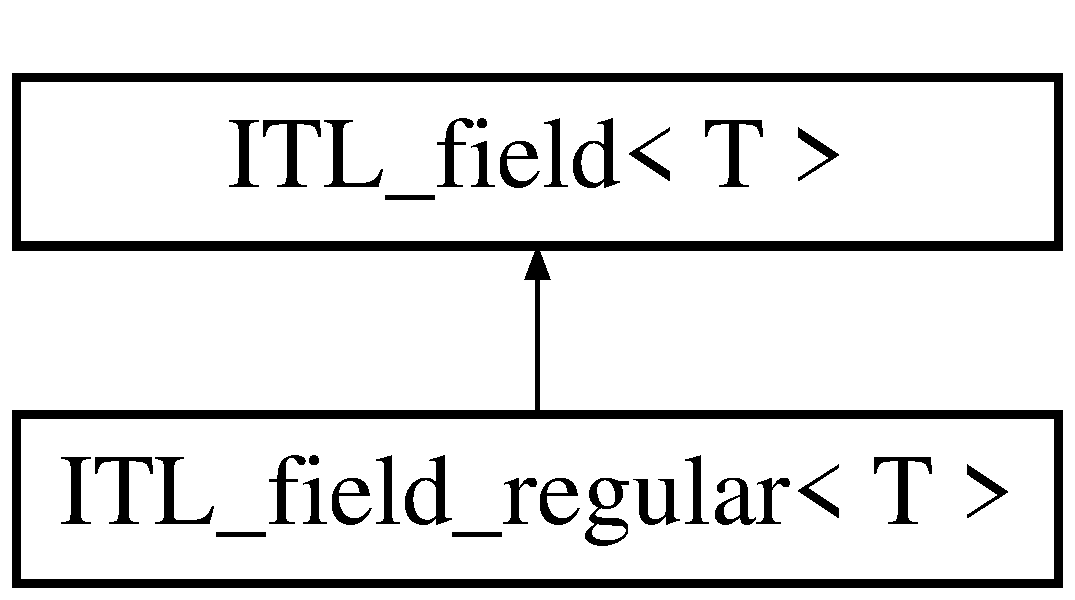
\includegraphics[height=2cm]{classITL__field__regular}
\end{center}
\end{figure}
\subsection*{Public Member Functions}
\begin{DoxyCompactItemize}
\item 
\hyperlink{classITL__field__regular_aca410e01f42b3cfd6c0d6e326e1a1136}{ITL\_\-field\_\-regular} ()
\begin{DoxyCompactList}\small\item\em Default constructor. \item\end{DoxyCompactList}\item 
\hyperlink{classITL__field__regular_abd45e2ed6be99bf2b5a058e39a47b18d}{ITL\_\-field\_\-regular} (T $\ast$\hyperlink{MainIT__regvector_8cpp_a783b2b1c03f80ec0d3ed965238d6bd65}{data}, int ndim, int $\ast$dim)
\begin{DoxyCompactList}\small\item\em Constructor type 2. \item\end{DoxyCompactList}\item 
\hyperlink{classITL__field__regular_ab01f00953429120f8e31152c69852163}{ITL\_\-field\_\-regular} (T $\ast$\hyperlink{MainIT__regvector_8cpp_a783b2b1c03f80ec0d3ed965238d6bd65}{data}, int ndim, float $\ast$l, float $\ast$h, int $\ast$lPad, int $\ast$hPad, int neighborhoodsize)
\begin{DoxyCompactList}\small\item\em Constructor type 3. \item\end{DoxyCompactList}\item 
\hyperlink{classITL__field__regular_aab02e2d45e98a9e8f861c448c30a319c}{ITL\_\-field\_\-regular} (T $\ast$\hyperlink{MainIT__regvector_8cpp_a783b2b1c03f80ec0d3ed965238d6bd65}{data}, int ndim, float $\ast$l, float $\ast$h, int $\ast$lPad, int $\ast$hPad, int $\ast$neighborhoodsizearray)
\item 
\hyperlink{classITL__field__regular_a4fb5a86290af1021054c96b1aed9d504}{ITL\_\-field\_\-regular} (int ndim, float $\ast$l, float $\ast$h)
\begin{DoxyCompactList}\small\item\em Constructor type 3. \item\end{DoxyCompactList}\item 
\hyperlink{classITL__field__regular_a0f0e50f05a38f12596faf9a6fc6a8674}{ITL\_\-field\_\-regular} (int ndim, float $\ast$l, float $\ast$h, int $\ast$lPad, int $\ast$hPad, int neighborhoodsize)
\begin{DoxyCompactList}\small\item\em Constructor type 4. \item\end{DoxyCompactList}\item 
\hyperlink{classITL__field__regular_aeabd017636d10eababa418b8cfa8765c}{ITL\_\-field\_\-regular} (int ndim, float $\ast$l, float $\ast$h, int $\ast$lPad, int $\ast$hPad, int $\ast$neighborhoodsizearray)
\item 
void \hyperlink{classITL__field__regular_a96d8e5cc41ae4e63671d43764056d161}{setBounds} (float $\ast$l, float $\ast$h)
\begin{DoxyCompactList}\small\item\em Pure virtual function for setting the bounds of a field with no ghost layers. \item\end{DoxyCompactList}\item 
void \hyperlink{classITL__field__regular_aa7897cdf06b261236e0efdab0987be9f}{setBounds} (float $\ast$l, float $\ast$h, int $\ast$lPad, int $\ast$hPad, int neighborhoodsize)
\begin{DoxyCompactList}\small\item\em Pure virtual function for setting the bounds of a field with ghost layers. \item\end{DoxyCompactList}\item 
void \hyperlink{classITL__field__regular_af208eb6a35d5be3d496ff110f56e62d0}{setBounds} (float $\ast$l, float $\ast$h, int $\ast$lPad, int $\ast$hPad, int $\ast$neighborhoodsizearray)
\item 
virtual void \hyperlink{classITL__field__regular_a0497909739ef494ee78808bbbfeaba0f}{partitionField} (int $\ast$nblocks)
\begin{DoxyCompactList}\small\item\em Function for creating a partition or subfield within the specified bounds. \item\end{DoxyCompactList}\item 
\hyperlink{classITL__field}{ITL\_\-field}$<$ T $>$ $\ast$ \hyperlink{classITL__field__regular_a600a5a99a3e696c3a6698f112933a90c}{createSubField} (float $\ast$\hyperlink{MainIT__regvector_8cpp_abb1e2dad97264e859f3ee8af1341d68c}{low}, float $\ast$\hyperlink{MainIT__regvector_8cpp_a2012a18ba7a98e566c072356d03c4240}{high})
\begin{DoxyCompactList}\small\item\em Function for creating a partition or subfield within the specified bounds. \item\end{DoxyCompactList}\item 
virtual T \hyperlink{classITL__field__regular_a78f814d7617aeb01c63def2f5f2e9caa}{getDataAt} (int id)
\begin{DoxyCompactList}\small\item\em Data accessor function type 1. \item\end{DoxyCompactList}\item 
virtual T \hyperlink{classITL__field__regular_ad05668c219a4632a3ceaca8409339103}{getDataAt} (int x, int y, int z)
\begin{DoxyCompactList}\small\item\em Data accessor function type 2. \item\end{DoxyCompactList}\item 
virtual T $\ast$ \hyperlink{classITL__field__regular_a13a2ec8f1e67b6a906d1799a58acf9bd}{getDataBetween} (float $\ast$lowBoundary, float $\ast$highBoundary)
\begin{DoxyCompactList}\small\item\em Data accessor function type 3. \item\end{DoxyCompactList}\item 
virtual T $\ast$ \hyperlink{classITL__field__regular_af0d8776246431db1f5069f2ce6eb4d2f}{getDataBetween} (int $\ast$lowBoundary, int $\ast$highBoundary)
\begin{DoxyCompactList}\small\item\em Data accessor function type 4. \item\end{DoxyCompactList}\item 
virtual T $\ast$ \hyperlink{classITL__field__regular_ac1e68a90b1eb23279aa18e5827102b2e}{getDataFull} ()
\begin{DoxyCompactList}\small\item\em Data accessor function type 5. \item\end{DoxyCompactList}\item 
virtual void \hyperlink{classITL__field__regular_a201a4f3e6b1a0ff6654f2bfbb40f516d}{setDataAt} (int id, T \hyperlink{MainIT__regvector_8cpp_a783b2b1c03f80ec0d3ed965238d6bd65}{data})
\begin{DoxyCompactList}\small\item\em Data mutator function type 1. \item\end{DoxyCompactList}\item 
virtual void \hyperlink{classITL__field__regular_a38fef3e9ec1551e58d217dcb29bcbc4b}{setDataAt} (int x, int y, int z, T \hyperlink{MainIT__regvector_8cpp_a783b2b1c03f80ec0d3ed965238d6bd65}{data})
\begin{DoxyCompactList}\small\item\em Data mutator function type 2. \item\end{DoxyCompactList}\item 
virtual void \hyperlink{classITL__field__regular_a07a0497a570f77755528aa9fc1e50934}{setDataBetween} (T $\ast$\hyperlink{MainIT__regvector_8cpp_a783b2b1c03f80ec0d3ed965238d6bd65}{data})
\begin{DoxyCompactList}\small\item\em Data mutator function type 3. \item\end{DoxyCompactList}\item 
virtual void \hyperlink{classITL__field__regular_aff339caac0e4e04156553b6b1c194fea}{setDataFull} (T $\ast$\hyperlink{MainIT__regvector_8cpp_a783b2b1c03f80ec0d3ed965238d6bd65}{data})
\begin{DoxyCompactList}\small\item\em Data mutator function type 4. \item\end{DoxyCompactList}\item 
\hyperlink{classITL__field__regular_a61df91153315ad7033658ab3fe811c25}{$\sim$ITL\_\-field\_\-regular} ()
\begin{DoxyCompactList}\small\item\em Destructor. \item\end{DoxyCompactList}\end{DoxyCompactItemize}


\subsection{Detailed Description}
\subsubsection*{template$<$class T$>$ class ITL\_\-field\_\-regular$<$ T $>$}

Regular field class inherited from \hyperlink{classITL__field}{ITL\_\-field}. Container for regularly arranged static/time-\/varying scalar/vector data. Created on: Dec 09, 2010 \begin{DoxyAuthor}{Author}
Abon 

Teng-\/Yok 
\end{DoxyAuthor}
\begin{DoxySeeAlso}{See also}
\hyperlink{classITL__field}{ITL\_\-field} 
\end{DoxySeeAlso}


Definition at line 17 of file ITL\_\-field\_\-regular.h.



\subsection{Constructor \& Destructor Documentation}
\hypertarget{classITL__field__regular_aca410e01f42b3cfd6c0d6e326e1a1136}{
\index{ITL\_\-field\_\-regular@{ITL\_\-field\_\-regular}!ITL\_\-field\_\-regular@{ITL\_\-field\_\-regular}}
\index{ITL\_\-field\_\-regular@{ITL\_\-field\_\-regular}!ITL_field_regular@{ITL\_\-field\_\-regular}}
\subsubsection[{ITL\_\-field\_\-regular}]{\setlength{\rightskip}{0pt plus 5cm}template$<$class T$>$ {\bf ITL\_\-field\_\-regular}$<$ T $>$::{\bf ITL\_\-field\_\-regular} ()\hspace{0.3cm}{\ttfamily  \mbox{[}inline\mbox{]}}}}
\label{classITL__field__regular_aca410e01f42b3cfd6c0d6e326e1a1136}


Default constructor. 



Definition at line 24 of file ITL\_\-field\_\-regular.h.

\hypertarget{classITL__field__regular_abd45e2ed6be99bf2b5a058e39a47b18d}{
\index{ITL\_\-field\_\-regular@{ITL\_\-field\_\-regular}!ITL\_\-field\_\-regular@{ITL\_\-field\_\-regular}}
\index{ITL\_\-field\_\-regular@{ITL\_\-field\_\-regular}!ITL_field_regular@{ITL\_\-field\_\-regular}}
\subsubsection[{ITL\_\-field\_\-regular}]{\setlength{\rightskip}{0pt plus 5cm}template$<$class T$>$ {\bf ITL\_\-field\_\-regular}$<$ T $>$::{\bf ITL\_\-field\_\-regular} (T $\ast$ {\em data}, \/  int {\em ndim}, \/  int $\ast$ {\em dim})\hspace{0.3cm}{\ttfamily  \mbox{[}inline\mbox{]}}}}
\label{classITL__field__regular_abd45e2ed6be99bf2b5a058e39a47b18d}


Constructor type 2. 


\begin{DoxyParams}{Parameters}
\item[{\em data}]pointer to 1D array of elements. \item[{\em ndim}]Dimensionality of field. \item[{\em dim}]Length of field along each dimension. \end{DoxyParams}


Definition at line 34 of file ITL\_\-field\_\-regular.h.

\hypertarget{classITL__field__regular_ab01f00953429120f8e31152c69852163}{
\index{ITL\_\-field\_\-regular@{ITL\_\-field\_\-regular}!ITL\_\-field\_\-regular@{ITL\_\-field\_\-regular}}
\index{ITL\_\-field\_\-regular@{ITL\_\-field\_\-regular}!ITL_field_regular@{ITL\_\-field\_\-regular}}
\subsubsection[{ITL\_\-field\_\-regular}]{\setlength{\rightskip}{0pt plus 5cm}template$<$class T$>$ {\bf ITL\_\-field\_\-regular}$<$ T $>$::{\bf ITL\_\-field\_\-regular} (T $\ast$ {\em data}, \/  int {\em ndim}, \/  float $\ast$ {\em l}, \/  float $\ast$ {\em h}, \/  int $\ast$ {\em lPad}, \/  int $\ast$ {\em hPad}, \/  int {\em neighborhoodsize})\hspace{0.3cm}{\ttfamily  \mbox{[}inline\mbox{]}}}}
\label{classITL__field__regular_ab01f00953429120f8e31152c69852163}


Constructor type 3. 


\begin{DoxyParams}{Parameters}
\item[{\em data}]pointer to 1D array of elements. \item[{\em ndim}]Dimensionality of field. \item[{\em dim}]Length of field along each dimension. \item[{\em l}]Pointer to array containing lower grid (associated to the field) bounds in continuous space along each dimension. \item[{\em h}]Pointer to array containing upper grid (associated to the field) bounds in continuous space along each dimension. \item[{\em lPad}]Pointer to array containing ghost layer span along each dimension on the lower end. \item[{\em hPad}]Pointer to array containing ghost layer span along each dimension on the upper end. \item[{\em neighborhoodsize}]Neighborhood length for each point. \end{DoxyParams}


Definition at line 65 of file ITL\_\-field\_\-regular.h.

\hypertarget{classITL__field__regular_aab02e2d45e98a9e8f861c448c30a319c}{
\index{ITL\_\-field\_\-regular@{ITL\_\-field\_\-regular}!ITL\_\-field\_\-regular@{ITL\_\-field\_\-regular}}
\index{ITL\_\-field\_\-regular@{ITL\_\-field\_\-regular}!ITL_field_regular@{ITL\_\-field\_\-regular}}
\subsubsection[{ITL\_\-field\_\-regular}]{\setlength{\rightskip}{0pt plus 5cm}template$<$class T$>$ {\bf ITL\_\-field\_\-regular}$<$ T $>$::{\bf ITL\_\-field\_\-regular} (T $\ast$ {\em data}, \/  int {\em ndim}, \/  float $\ast$ {\em l}, \/  float $\ast$ {\em h}, \/  int $\ast$ {\em lPad}, \/  int $\ast$ {\em hPad}, \/  int $\ast$ {\em neighborhoodsizearray})\hspace{0.3cm}{\ttfamily  \mbox{[}inline\mbox{]}}}}
\label{classITL__field__regular_aab02e2d45e98a9e8f861c448c30a319c}


Definition at line 78 of file ITL\_\-field\_\-regular.h.

\hypertarget{classITL__field__regular_a4fb5a86290af1021054c96b1aed9d504}{
\index{ITL\_\-field\_\-regular@{ITL\_\-field\_\-regular}!ITL\_\-field\_\-regular@{ITL\_\-field\_\-regular}}
\index{ITL\_\-field\_\-regular@{ITL\_\-field\_\-regular}!ITL_field_regular@{ITL\_\-field\_\-regular}}
\subsubsection[{ITL\_\-field\_\-regular}]{\setlength{\rightskip}{0pt plus 5cm}template$<$class T$>$ {\bf ITL\_\-field\_\-regular}$<$ T $>$::{\bf ITL\_\-field\_\-regular} (int {\em ndim}, \/  float $\ast$ {\em l}, \/  float $\ast$ {\em h})\hspace{0.3cm}{\ttfamily  \mbox{[}inline\mbox{]}}}}
\label{classITL__field__regular_a4fb5a86290af1021054c96b1aed9d504}


Constructor type 3. 


\begin{DoxyParams}{Parameters}
\item[{\em ndim}]Dimensionality of field. \item[{\em l}]Pointer to array containing lower grid (associated to the field) bounds in continuous space along each dimension. \item[{\em h}]Pointer to array containing upper grid (associated to the field) bounds in continuous space along each dimension. \end{DoxyParams}


Definition at line 97 of file ITL\_\-field\_\-regular.h.

\hypertarget{classITL__field__regular_a0f0e50f05a38f12596faf9a6fc6a8674}{
\index{ITL\_\-field\_\-regular@{ITL\_\-field\_\-regular}!ITL\_\-field\_\-regular@{ITL\_\-field\_\-regular}}
\index{ITL\_\-field\_\-regular@{ITL\_\-field\_\-regular}!ITL_field_regular@{ITL\_\-field\_\-regular}}
\subsubsection[{ITL\_\-field\_\-regular}]{\setlength{\rightskip}{0pt plus 5cm}template$<$class T$>$ {\bf ITL\_\-field\_\-regular}$<$ T $>$::{\bf ITL\_\-field\_\-regular} (int {\em ndim}, \/  float $\ast$ {\em l}, \/  float $\ast$ {\em h}, \/  int $\ast$ {\em lPad}, \/  int $\ast$ {\em hPad}, \/  int {\em neighborhoodsize})\hspace{0.3cm}{\ttfamily  \mbox{[}inline\mbox{]}}}}
\label{classITL__field__regular_a0f0e50f05a38f12596faf9a6fc6a8674}


Constructor type 4. 


\begin{DoxyParams}{Parameters}
\item[{\em ndim}]Dimensionality of field. \item[{\em l}]Pointer to array containing lower grid (associated to the field) bounds in continuous space along each dimension. \item[{\em h}]Pointer to array containing upper grid (associated to the field) bounds in continuous space along each dimension. \item[{\em lPad}]Pointer to array containing ghost layer span along each dimension on the lower end. \item[{\em hPad}]Pointer to array containing ghost layer span along each dimension on the upper end. \item[{\em neighborhoodsize}]Neighborhood length for each point. \end{DoxyParams}


Definition at line 119 of file ITL\_\-field\_\-regular.h.

\hypertarget{classITL__field__regular_aeabd017636d10eababa418b8cfa8765c}{
\index{ITL\_\-field\_\-regular@{ITL\_\-field\_\-regular}!ITL\_\-field\_\-regular@{ITL\_\-field\_\-regular}}
\index{ITL\_\-field\_\-regular@{ITL\_\-field\_\-regular}!ITL_field_regular@{ITL\_\-field\_\-regular}}
\subsubsection[{ITL\_\-field\_\-regular}]{\setlength{\rightskip}{0pt plus 5cm}template$<$class T$>$ {\bf ITL\_\-field\_\-regular}$<$ T $>$::{\bf ITL\_\-field\_\-regular} (int {\em ndim}, \/  float $\ast$ {\em l}, \/  float $\ast$ {\em h}, \/  int $\ast$ {\em lPad}, \/  int $\ast$ {\em hPad}, \/  int $\ast$ {\em neighborhoodsizearray})\hspace{0.3cm}{\ttfamily  \mbox{[}inline\mbox{]}}}}
\label{classITL__field__regular_aeabd017636d10eababa418b8cfa8765c}


Definition at line 132 of file ITL\_\-field\_\-regular.h.

\hypertarget{classITL__field__regular_a61df91153315ad7033658ab3fe811c25}{
\index{ITL\_\-field\_\-regular@{ITL\_\-field\_\-regular}!$\sim$ITL\_\-field\_\-regular@{$\sim$ITL\_\-field\_\-regular}}
\index{$\sim$ITL\_\-field\_\-regular@{$\sim$ITL\_\-field\_\-regular}!ITL_field_regular@{ITL\_\-field\_\-regular}}
\subsubsection[{$\sim$ITL\_\-field\_\-regular}]{\setlength{\rightskip}{0pt plus 5cm}template$<$class T$>$ {\bf ITL\_\-field\_\-regular}$<$ T $>$::$\sim${\bf ITL\_\-field\_\-regular} ()\hspace{0.3cm}{\ttfamily  \mbox{[}inline\mbox{]}}}}
\label{classITL__field__regular_a61df91153315ad7033658ab3fe811c25}


Destructor. 



Definition at line 405 of file ITL\_\-field\_\-regular.h.



\subsection{Member Function Documentation}
\hypertarget{classITL__field__regular_a600a5a99a3e696c3a6698f112933a90c}{
\index{ITL\_\-field\_\-regular@{ITL\_\-field\_\-regular}!createSubField@{createSubField}}
\index{createSubField@{createSubField}!ITL_field_regular@{ITL\_\-field\_\-regular}}
\subsubsection[{createSubField}]{\setlength{\rightskip}{0pt plus 5cm}template$<$class T$>$ {\bf ITL\_\-field}$<$T$>$$\ast$ {\bf ITL\_\-field\_\-regular}$<$ T $>$::createSubField (float $\ast$ {\em low}, \/  float $\ast$ {\em high})\hspace{0.3cm}{\ttfamily  \mbox{[}inline, virtual\mbox{]}}}}
\label{classITL__field__regular_a600a5a99a3e696c3a6698f112933a90c}


Function for creating a partition or subfield within the specified bounds. 


\begin{DoxyParams}{Parameters}
\item[{\em low}]Lower bound along each dimension. \item[{\em high}]Higher bound along each dimension. \end{DoxyParams}


Reimplemented from \hyperlink{classITL__field_a7ca32e8dd6186974778ae4c8302ee922}{ITL\_\-field$<$ T $>$}.



Definition at line 249 of file ITL\_\-field\_\-regular.h.

\hypertarget{classITL__field__regular_ad05668c219a4632a3ceaca8409339103}{
\index{ITL\_\-field\_\-regular@{ITL\_\-field\_\-regular}!getDataAt@{getDataAt}}
\index{getDataAt@{getDataAt}!ITL_field_regular@{ITL\_\-field\_\-regular}}
\subsubsection[{getDataAt}]{\setlength{\rightskip}{0pt plus 5cm}template$<$class T$>$ virtual T {\bf ITL\_\-field\_\-regular}$<$ T $>$::getDataAt (int {\em x}, \/  int {\em y}, \/  int {\em z})\hspace{0.3cm}{\ttfamily  \mbox{[}inline, virtual\mbox{]}}}}
\label{classITL__field__regular_ad05668c219a4632a3ceaca8409339103}


Data accessor function type 2. 


\begin{DoxyParams}{Parameters}
\item[{\em x}]x-\/coordinate of the spatial point. \item[{\em y}]y-\/coordinate of the spatial point. \item[{\em z}]z-\/coordinate of the spatial point. \end{DoxyParams}
\begin{DoxyReturn}{Returns}
field value. 
\end{DoxyReturn}


Reimplemented from \hyperlink{classITL__field_a40f9224e8815388882c953b914c540ff}{ITL\_\-field$<$ T $>$}.



Definition at line 285 of file ITL\_\-field\_\-regular.h.

\hypertarget{classITL__field__regular_a78f814d7617aeb01c63def2f5f2e9caa}{
\index{ITL\_\-field\_\-regular@{ITL\_\-field\_\-regular}!getDataAt@{getDataAt}}
\index{getDataAt@{getDataAt}!ITL_field_regular@{ITL\_\-field\_\-regular}}
\subsubsection[{getDataAt}]{\setlength{\rightskip}{0pt plus 5cm}template$<$class T$>$ virtual T {\bf ITL\_\-field\_\-regular}$<$ T $>$::getDataAt (int {\em id})\hspace{0.3cm}{\ttfamily  \mbox{[}inline, virtual\mbox{]}}}}
\label{classITL__field__regular_a78f814d7617aeb01c63def2f5f2e9caa}


Data accessor function type 1. 


\begin{DoxyParams}{Parameters}
\item[{\em id}]1D index of data array \end{DoxyParams}
\begin{DoxyReturn}{Returns}
field value. 
\end{DoxyReturn}


Reimplemented from \hyperlink{classITL__field_a9a4b41fbeafd49afde45b608b5db2c09}{ITL\_\-field$<$ T $>$}.



Definition at line 272 of file ITL\_\-field\_\-regular.h.

\hypertarget{classITL__field__regular_af0d8776246431db1f5069f2ce6eb4d2f}{
\index{ITL\_\-field\_\-regular@{ITL\_\-field\_\-regular}!getDataBetween@{getDataBetween}}
\index{getDataBetween@{getDataBetween}!ITL_field_regular@{ITL\_\-field\_\-regular}}
\subsubsection[{getDataBetween}]{\setlength{\rightskip}{0pt plus 5cm}template$<$class T$>$ virtual T$\ast$ {\bf ITL\_\-field\_\-regular}$<$ T $>$::getDataBetween (int $\ast$ {\em lowBoundary}, \/  int $\ast$ {\em highBoundary})\hspace{0.3cm}{\ttfamily  \mbox{[}inline, virtual\mbox{]}}}}
\label{classITL__field__regular_af0d8776246431db1f5069f2ce6eb4d2f}


Data accessor function type 4. 

Returns chunk of data within specified bound. 
\begin{DoxyParams}{Parameters}
\item[{\em lowBoundary}]Lower bound along each dimension. \item[{\em highBoundary}]Higher bound along each dimension. \end{DoxyParams}
\begin{DoxyReturn}{Returns}
pointer to field value. 
\end{DoxyReturn}


Reimplemented from \hyperlink{classITL__field_ab3254f696ccca1b4ea1aae248bea989c}{ITL\_\-field$<$ T $>$}.



Definition at line 323 of file ITL\_\-field\_\-regular.h.

\hypertarget{classITL__field__regular_a13a2ec8f1e67b6a906d1799a58acf9bd}{
\index{ITL\_\-field\_\-regular@{ITL\_\-field\_\-regular}!getDataBetween@{getDataBetween}}
\index{getDataBetween@{getDataBetween}!ITL_field_regular@{ITL\_\-field\_\-regular}}
\subsubsection[{getDataBetween}]{\setlength{\rightskip}{0pt plus 5cm}template$<$class T$>$ virtual T$\ast$ {\bf ITL\_\-field\_\-regular}$<$ T $>$::getDataBetween (float $\ast$ {\em lowBoundary}, \/  float $\ast$ {\em highBoundary})\hspace{0.3cm}{\ttfamily  \mbox{[}inline, virtual\mbox{]}}}}
\label{classITL__field__regular_a13a2ec8f1e67b6a906d1799a58acf9bd}


Data accessor function type 3. 

Returns chunk of data within specified bound. 
\begin{DoxyParams}{Parameters}
\item[{\em lowBoundary}]Lower bound along each dimension. \item[{\em highBoundary}]Higher bound along each dimension. \end{DoxyParams}
\begin{DoxyReturn}{Returns}
pointer to field value. 
\end{DoxyReturn}


Reimplemented from \hyperlink{classITL__field_a983bd8b95e95bf758a73fafccea62a49}{ITL\_\-field$<$ T $>$}.



Definition at line 301 of file ITL\_\-field\_\-regular.h.

\hypertarget{classITL__field__regular_ac1e68a90b1eb23279aa18e5827102b2e}{
\index{ITL\_\-field\_\-regular@{ITL\_\-field\_\-regular}!getDataFull@{getDataFull}}
\index{getDataFull@{getDataFull}!ITL_field_regular@{ITL\_\-field\_\-regular}}
\subsubsection[{getDataFull}]{\setlength{\rightskip}{0pt plus 5cm}template$<$class T$>$ virtual T$\ast$ {\bf ITL\_\-field\_\-regular}$<$ T $>$::getDataFull ()\hspace{0.3cm}{\ttfamily  \mbox{[}inline, virtual\mbox{]}}}}
\label{classITL__field__regular_ac1e68a90b1eb23279aa18e5827102b2e}


Data accessor function type 5. 

Returns entire field data. \begin{DoxyReturn}{Returns}
pointer to field value. 
\end{DoxyReturn}


Reimplemented from \hyperlink{classITL__field_afba4c040443d3f21d3f4af30a70292be}{ITL\_\-field$<$ T $>$}.



Definition at line 355 of file ITL\_\-field\_\-regular.h.

\hypertarget{classITL__field__regular_a0497909739ef494ee78808bbbfeaba0f}{
\index{ITL\_\-field\_\-regular@{ITL\_\-field\_\-regular}!partitionField@{partitionField}}
\index{partitionField@{partitionField}!ITL_field_regular@{ITL\_\-field\_\-regular}}
\subsubsection[{partitionField}]{\setlength{\rightskip}{0pt plus 5cm}template$<$class T$>$ virtual void {\bf ITL\_\-field\_\-regular}$<$ T $>$::partitionField (int $\ast$ {\em nblocks})\hspace{0.3cm}{\ttfamily  \mbox{[}inline, virtual\mbox{]}}}}
\label{classITL__field__regular_a0497909739ef494ee78808bbbfeaba0f}


Function for creating a partition or subfield within the specified bounds. 


\begin{DoxyParams}{Parameters}
\item[{\em nblocks}]Number of partitions along each dimension. \end{DoxyParams}


Reimplemented from \hyperlink{classITL__field_a5c7ecb94890c0dd7d730e881f530bbc2}{ITL\_\-field$<$ T $>$}.



Definition at line 187 of file ITL\_\-field\_\-regular.h.

\hypertarget{classITL__field__regular_af208eb6a35d5be3d496ff110f56e62d0}{
\index{ITL\_\-field\_\-regular@{ITL\_\-field\_\-regular}!setBounds@{setBounds}}
\index{setBounds@{setBounds}!ITL_field_regular@{ITL\_\-field\_\-regular}}
\subsubsection[{setBounds}]{\setlength{\rightskip}{0pt plus 5cm}template$<$class T$>$ void {\bf ITL\_\-field\_\-regular}$<$ T $>$::setBounds (float $\ast$ {\em l}, \/  float $\ast$ {\em h}, \/  int $\ast$ {\em lPad}, \/  int $\ast$ {\em hPad}, \/  int $\ast$ {\em neighborhoodsizearray})\hspace{0.3cm}{\ttfamily  \mbox{[}inline\mbox{]}}}}
\label{classITL__field__regular_af208eb6a35d5be3d496ff110f56e62d0}


Definition at line 175 of file ITL\_\-field\_\-regular.h.

\hypertarget{classITL__field__regular_aa7897cdf06b261236e0efdab0987be9f}{
\index{ITL\_\-field\_\-regular@{ITL\_\-field\_\-regular}!setBounds@{setBounds}}
\index{setBounds@{setBounds}!ITL_field_regular@{ITL\_\-field\_\-regular}}
\subsubsection[{setBounds}]{\setlength{\rightskip}{0pt plus 5cm}template$<$class T$>$ void {\bf ITL\_\-field\_\-regular}$<$ T $>$::setBounds (float $\ast$ {\em l}, \/  float $\ast$ {\em h}, \/  int $\ast$ {\em lPad}, \/  int $\ast$ {\em hPad}, \/  int {\em neighborhoodsize})\hspace{0.3cm}{\ttfamily  \mbox{[}inline, virtual\mbox{]}}}}
\label{classITL__field__regular_aa7897cdf06b261236e0efdab0987be9f}


Pure virtual function for setting the bounds of a field with ghost layers. 

Calls corresponding function of the grid. 
\begin{DoxyParams}{Parameters}
\item[{\em l}]Pointer to array containing lower grid (associated to the field) bounds in continuous space along each dimension. \item[{\em h}]Pointer to array containing upper grid (associated to the field) bounds in continuous space along each dimension. \item[{\em lPad}]Pointer to array containing ghost layer span along each dimension on the lower end. \item[{\em hPad}]Pointer to array containing ghost layer span along each dimension on the upper end. \item[{\em neighborhoodsize}]Neighborhood length for each point. \end{DoxyParams}


Reimplemented from \hyperlink{classITL__field_ab27b49b81f3a7a2a614eaca91cd8eb8c}{ITL\_\-field$<$ T $>$}.



Definition at line 168 of file ITL\_\-field\_\-regular.h.

\hypertarget{classITL__field__regular_a96d8e5cc41ae4e63671d43764056d161}{
\index{ITL\_\-field\_\-regular@{ITL\_\-field\_\-regular}!setBounds@{setBounds}}
\index{setBounds@{setBounds}!ITL_field_regular@{ITL\_\-field\_\-regular}}
\subsubsection[{setBounds}]{\setlength{\rightskip}{0pt plus 5cm}template$<$class T$>$ void {\bf ITL\_\-field\_\-regular}$<$ T $>$::setBounds (float $\ast$ {\em l}, \/  float $\ast$ {\em h})\hspace{0.3cm}{\ttfamily  \mbox{[}inline, virtual\mbox{]}}}}
\label{classITL__field__regular_a96d8e5cc41ae4e63671d43764056d161}


Pure virtual function for setting the bounds of a field with no ghost layers. 

Calls corresponding function of the grid. 
\begin{DoxyParams}{Parameters}
\item[{\em l}]Pointer to array containing lower grid (associated to the field) bounds in continuous space along each dimension. \item[{\em h}]Pointer to array containing upper grid (associated to the field) bounds in continuous space along each dimension. \end{DoxyParams}


Reimplemented from \hyperlink{classITL__field_a7bf82ed82a338d34985a6758307c8ece}{ITL\_\-field$<$ T $>$}.



Definition at line 152 of file ITL\_\-field\_\-regular.h.

\hypertarget{classITL__field__regular_a38fef3e9ec1551e58d217dcb29bcbc4b}{
\index{ITL\_\-field\_\-regular@{ITL\_\-field\_\-regular}!setDataAt@{setDataAt}}
\index{setDataAt@{setDataAt}!ITL_field_regular@{ITL\_\-field\_\-regular}}
\subsubsection[{setDataAt}]{\setlength{\rightskip}{0pt plus 5cm}template$<$class T$>$ virtual void {\bf ITL\_\-field\_\-regular}$<$ T $>$::setDataAt (int {\em x}, \/  int {\em y}, \/  int {\em z}, \/  T {\em data})\hspace{0.3cm}{\ttfamily  \mbox{[}inline, virtual\mbox{]}}}}
\label{classITL__field__regular_a38fef3e9ec1551e58d217dcb29bcbc4b}


Data mutator function type 2. 



Reimplemented from \hyperlink{classITL__field_aeea532e25732eb1582a937409a98d05e}{ITL\_\-field$<$ T $>$}.



Definition at line 375 of file ITL\_\-field\_\-regular.h.

\hypertarget{classITL__field__regular_a201a4f3e6b1a0ff6654f2bfbb40f516d}{
\index{ITL\_\-field\_\-regular@{ITL\_\-field\_\-regular}!setDataAt@{setDataAt}}
\index{setDataAt@{setDataAt}!ITL_field_regular@{ITL\_\-field\_\-regular}}
\subsubsection[{setDataAt}]{\setlength{\rightskip}{0pt plus 5cm}template$<$class T$>$ virtual void {\bf ITL\_\-field\_\-regular}$<$ T $>$::setDataAt (int {\em id}, \/  T {\em data})\hspace{0.3cm}{\ttfamily  \mbox{[}inline, virtual\mbox{]}}}}
\label{classITL__field__regular_a201a4f3e6b1a0ff6654f2bfbb40f516d}


Data mutator function type 1. 

Sets data at a particular array location. 
\begin{DoxyParams}{Parameters}
\item[{\em id}]1D index of data array \item[{\em data}]field value. \end{DoxyParams}


Reimplemented from \hyperlink{classITL__field_ae87ee8fef9c9b9dc6a782ccbfe3605e1}{ITL\_\-field$<$ T $>$}.



Definition at line 366 of file ITL\_\-field\_\-regular.h.

\hypertarget{classITL__field__regular_a07a0497a570f77755528aa9fc1e50934}{
\index{ITL\_\-field\_\-regular@{ITL\_\-field\_\-regular}!setDataBetween@{setDataBetween}}
\index{setDataBetween@{setDataBetween}!ITL_field_regular@{ITL\_\-field\_\-regular}}
\subsubsection[{setDataBetween}]{\setlength{\rightskip}{0pt plus 5cm}template$<$class T$>$ virtual void {\bf ITL\_\-field\_\-regular}$<$ T $>$::setDataBetween (T $\ast$ {\em data})\hspace{0.3cm}{\ttfamily  \mbox{[}inline, virtual\mbox{]}}}}
\label{classITL__field__regular_a07a0497a570f77755528aa9fc1e50934}


Data mutator function type 3. 



Reimplemented from \hyperlink{classITL__field_a4bbd5103c5298ac87eaac25c759a98c7}{ITL\_\-field$<$ T $>$}.



Definition at line 387 of file ITL\_\-field\_\-regular.h.

\hypertarget{classITL__field__regular_aff339caac0e4e04156553b6b1c194fea}{
\index{ITL\_\-field\_\-regular@{ITL\_\-field\_\-regular}!setDataFull@{setDataFull}}
\index{setDataFull@{setDataFull}!ITL_field_regular@{ITL\_\-field\_\-regular}}
\subsubsection[{setDataFull}]{\setlength{\rightskip}{0pt plus 5cm}template$<$class T$>$ virtual void {\bf ITL\_\-field\_\-regular}$<$ T $>$::setDataFull (T $\ast$ {\em data})\hspace{0.3cm}{\ttfamily  \mbox{[}inline, virtual\mbox{]}}}}
\label{classITL__field__regular_aff339caac0e4e04156553b6b1c194fea}


Data mutator function type 4. 

Sets data for entire field. 
\begin{DoxyParams}{Parameters}
\item[{\em data}]pointer to data \end{DoxyParams}


Reimplemented from \hyperlink{classITL__field_a0c32994fe56253d8c7111d670742afc1}{ITL\_\-field$<$ T $>$}.



Definition at line 397 of file ITL\_\-field\_\-regular.h.



The documentation for this class was generated from the following file:\begin{DoxyCompactItemize}
\item 
/home/abon/Code/workspace\_\-unix/ITL\_\-repo/include/\hyperlink{ITL__field__regular_8h}{ITL\_\-field\_\-regular.h}\end{DoxyCompactItemize}

\hypertarget{classITL__field__unstructured}{
\section{ITL\_\-field\_\-unstructured$<$ T $>$ Class Template Reference}
\label{classITL__field__unstructured}\index{ITL\_\-field\_\-unstructured@{ITL\_\-field\_\-unstructured}}
}


Unstructured field class inherited from \hyperlink{classITL__field}{ITL\_\-field}.  




{\ttfamily \#include $<$ITL\_\-field\_\-unstructured.h$>$}

Inheritance diagram for ITL\_\-field\_\-unstructured$<$ T $>$:\begin{figure}[H]
\begin{center}
\leavevmode
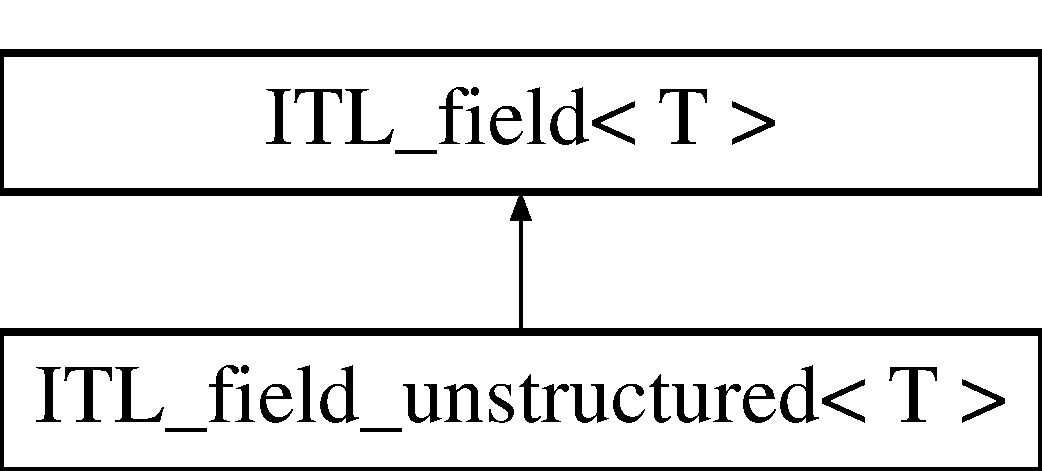
\includegraphics[height=2cm]{classITL__field__unstructured}
\end{center}
\end{figure}


\subsection{Detailed Description}
\subsubsection*{template$<$class T$>$ class ITL\_\-field\_\-unstructured$<$ T $>$}

Unstructured field class inherited from \hyperlink{classITL__field}{ITL\_\-field}. Container for irregularly spaced static/time-\/varying scalar/vector data. Created on: Dec 09, 2010 \begin{DoxyAuthor}{Author}
Abon 

Teng-\/Yok 
\end{DoxyAuthor}


Definition at line 13 of file ITL\_\-field\_\-unstructured.h.



The documentation for this class was generated from the following file:\begin{DoxyCompactItemize}
\item 
/home/abon/Code/workspace\_\-unix/ITL\_\-repo/include/\hyperlink{ITL__field__unstructured_8h}{ITL\_\-field\_\-unstructured.h}\end{DoxyCompactItemize}

\hypertarget{classITL__globalentropy}{
\section{ITL\_\-globalentropy$<$ T $>$ Class Template Reference}
\label{classITL__globalentropy}\index{ITL\_\-globalentropy@{ITL\_\-globalentropy}}
}


Gloabl entropy computation class.  




{\ttfamily \#include $<$ITL\_\-globalentropy.h$>$}

\subsection*{Public Member Functions}
\begin{DoxyCompactItemize}
\item 
\hyperlink{classITL__globalentropy_af82eb0ffa8d7d33ec3e3c6af95322cf2}{ITL\_\-globalentropy} (\hyperlink{classITL__field__regular}{ITL\_\-field\_\-regular}$<$ T $>$ $\ast$f)
\begin{DoxyCompactList}\small\item\em Default Constructor. \item\end{DoxyCompactList}\item 
void \hyperlink{classITL__globalentropy_afe13cb031dbfa959c547ac1a0d849472}{computeHistogramBinField} (char $\ast$fieldType, int \hyperlink{MainIT__regvector_8cpp_a7f13753d4707f6bc8f71d8bdacedefb3}{nBin}=0)
\begin{DoxyCompactList}\small\item\em Histogram bin assignment function. \item\end{DoxyCompactList}\item 
void \hyperlink{classITL__globalentropy_aad50922e014e3b5929e9415c8ddef382}{computeHistogramBinField\_\-Scalar} (int \hyperlink{MainIT__regvector_8cpp_a7f13753d4707f6bc8f71d8bdacedefb3}{nBin})
\begin{DoxyCompactList}\small\item\em Histogram bin assignment function for scalar fields. \item\end{DoxyCompactList}\item 
void \hyperlink{classITL__globalentropy_a6929e8efe91de1d1d604897ac1d1cb0f}{computeHistogramBinField\_\-Vector} (int \hyperlink{MainIT__regvector_8cpp_a7f13753d4707f6bc8f71d8bdacedefb3}{nBin})
\begin{DoxyCompactList}\small\item\em Histogram bin assignment function for vector fields. \item\end{DoxyCompactList}\item 
void \hyperlink{classITL__globalentropy_ad6e98f40d85501050f6a055bd8218525}{computeGlobalEntropyOfField} (int \hyperlink{MainIT__regvector_8cpp_a7f13753d4707f6bc8f71d8bdacedefb3}{nBin}, bool toNormalize, int \hyperlink{MainIT__regscalar_8cpp_adcc9a19ad3119f823a658f6a49a24e64}{method}=0)
\begin{DoxyCompactList}\small\item\em Entropy computation function. \item\end{DoxyCompactList}\item 
float \hyperlink{classITL__globalentropy_a971ff6f68ca3399c374f52f24bb1232c}{getGlobalEntropy} ()
\begin{DoxyCompactList}\small\item\em Entropy field accessor function. \item\end{DoxyCompactList}\end{DoxyCompactItemize}
\subsection*{Public Attributes}
\begin{DoxyCompactItemize}
\item 
\hyperlink{classITL__field__regular}{ITL\_\-field\_\-regular}$<$ T $>$ $\ast$ \hyperlink{classITL__globalentropy_adc0074ac722c23f71868d43ed818e063}{dataField}
\item 
\hyperlink{classITL__field__regular}{ITL\_\-field\_\-regular}$<$ int $>$ $\ast$ \hyperlink{classITL__globalentropy_ac546157f722e8b579c020180a0473ea0}{binData}
\begin{DoxyCompactList}\small\item\em A scalar field containing histogram bins corresponding to field points. \item\end{DoxyCompactList}\item 
float \hyperlink{classITL__globalentropy_a462d47cb4eb2b6b7dae04113db7f301a}{globalEntropy}
\begin{DoxyCompactList}\small\item\em Value of computed global entropy of the field. \item\end{DoxyCompactList}\item 
float $\ast$ \hyperlink{classITL__globalentropy_a65aa14c47161756fa3dd18b171c232f1}{probarray}
\begin{DoxyCompactList}\small\item\em Probability array used in entropy computation. \item\end{DoxyCompactList}\end{DoxyCompactItemize}


\subsection{Detailed Description}
\subsubsection*{template$<$class T$>$ class ITL\_\-globalentropy$<$ T $>$}

Gloabl entropy computation class. Created on: April 02, 2011. \begin{DoxyAuthor}{Author}
Abon 

Teng-\/Yok 
\end{DoxyAuthor}


Definition at line 16 of file ITL\_\-globalentropy.h.



\subsection{Constructor \& Destructor Documentation}
\hypertarget{classITL__globalentropy_af82eb0ffa8d7d33ec3e3c6af95322cf2}{
\index{ITL\_\-globalentropy@{ITL\_\-globalentropy}!ITL\_\-globalentropy@{ITL\_\-globalentropy}}
\index{ITL\_\-globalentropy@{ITL\_\-globalentropy}!ITL_globalentropy@{ITL\_\-globalentropy}}
\subsubsection[{ITL\_\-globalentropy}]{\setlength{\rightskip}{0pt plus 5cm}template$<$class T$>$ {\bf ITL\_\-globalentropy}$<$ T $>$::{\bf ITL\_\-globalentropy} ({\bf ITL\_\-field\_\-regular}$<$ T $>$ $\ast$ {\em f})\hspace{0.3cm}{\ttfamily  \mbox{[}inline\mbox{]}}}}
\label{classITL__globalentropy_af82eb0ffa8d7d33ec3e3c6af95322cf2}


Default Constructor. 



Definition at line 27 of file ITL\_\-globalentropy.h.



\subsection{Member Function Documentation}
\hypertarget{classITL__globalentropy_ad6e98f40d85501050f6a055bd8218525}{
\index{ITL\_\-globalentropy@{ITL\_\-globalentropy}!computeGlobalEntropyOfField@{computeGlobalEntropyOfField}}
\index{computeGlobalEntropyOfField@{computeGlobalEntropyOfField}!ITL_globalentropy@{ITL\_\-globalentropy}}
\subsubsection[{computeGlobalEntropyOfField}]{\setlength{\rightskip}{0pt plus 5cm}template$<$class T$>$ void {\bf ITL\_\-globalentropy}$<$ T $>$::computeGlobalEntropyOfField (int {\em nBin}, \/  bool {\em toNormalize}, \/  int {\em method} = {\ttfamily 0})\hspace{0.3cm}{\ttfamily  \mbox{[}inline\mbox{]}}}}
\label{classITL__globalentropy_ad6e98f40d85501050f6a055bd8218525}


Entropy computation function. 

Creates a scalar field that contains entropy at each grid vertex. 
\begin{DoxyParams}{Parameters}
\item[{\em nBins}]Number of bins used in histogram computation/Number of sample points in KDE estimation.  toNormalize boolean flag, TRUE indicates that the computed entropy value needs to be normalized \end{DoxyParams}


Definition at line 193 of file ITL\_\-globalentropy.h.

\hypertarget{classITL__globalentropy_afe13cb031dbfa959c547ac1a0d849472}{
\index{ITL\_\-globalentropy@{ITL\_\-globalentropy}!computeHistogramBinField@{computeHistogramBinField}}
\index{computeHistogramBinField@{computeHistogramBinField}!ITL_globalentropy@{ITL\_\-globalentropy}}
\subsubsection[{computeHistogramBinField}]{\setlength{\rightskip}{0pt plus 5cm}template$<$class T$>$ void {\bf ITL\_\-globalentropy}$<$ T $>$::computeHistogramBinField (char $\ast$ {\em fieldType}, \/  int {\em nBin} = {\ttfamily 0})\hspace{0.3cm}{\ttfamily  \mbox{[}inline\mbox{]}}}}
\label{classITL__globalentropy_afe13cb031dbfa959c547ac1a0d849472}


Histogram bin assignment function. 

Calls the appropriate function based on field type 
\begin{DoxyParams}{Parameters}
\item[{\em nBins}]Number of bins to use in histogram computation. \end{DoxyParams}


Definition at line 39 of file ITL\_\-globalentropy.h.

\hypertarget{classITL__globalentropy_aad50922e014e3b5929e9415c8ddef382}{
\index{ITL\_\-globalentropy@{ITL\_\-globalentropy}!computeHistogramBinField\_\-Scalar@{computeHistogramBinField\_\-Scalar}}
\index{computeHistogramBinField\_\-Scalar@{computeHistogramBinField\_\-Scalar}!ITL_globalentropy@{ITL\_\-globalentropy}}
\subsubsection[{computeHistogramBinField\_\-Scalar}]{\setlength{\rightskip}{0pt plus 5cm}template$<$class T$>$ void {\bf ITL\_\-globalentropy}$<$ T $>$::computeHistogramBinField\_\-Scalar (int {\em nBin})\hspace{0.3cm}{\ttfamily  \mbox{[}inline\mbox{]}}}}
\label{classITL__globalentropy_aad50922e014e3b5929e9415c8ddef382}


Histogram bin assignment function for scalar fields. 

Creates a scalar field of histogram at each grid vertex. 
\begin{DoxyParams}{Parameters}
\item[{\em nBins}]Number of bins to use in histogram computation. \end{DoxyParams}


Definition at line 62 of file ITL\_\-globalentropy.h.

\hypertarget{classITL__globalentropy_a6929e8efe91de1d1d604897ac1d1cb0f}{
\index{ITL\_\-globalentropy@{ITL\_\-globalentropy}!computeHistogramBinField\_\-Vector@{computeHistogramBinField\_\-Vector}}
\index{computeHistogramBinField\_\-Vector@{computeHistogramBinField\_\-Vector}!ITL_globalentropy@{ITL\_\-globalentropy}}
\subsubsection[{computeHistogramBinField\_\-Vector}]{\setlength{\rightskip}{0pt plus 5cm}template$<$class T$>$ void {\bf ITL\_\-globalentropy}$<$ T $>$::computeHistogramBinField\_\-Vector (int {\em nBin})\hspace{0.3cm}{\ttfamily  \mbox{[}inline\mbox{]}}}}
\label{classITL__globalentropy_a6929e8efe91de1d1d604897ac1d1cb0f}


Histogram bin assignment function for vector fields. 

Creates a scalar field of histogram at each grid vertex. 
\begin{DoxyParams}{Parameters}
\item[{\em nBins}]Number of bins to use in histogram computation. \end{DoxyParams}


Definition at line 135 of file ITL\_\-globalentropy.h.

\hypertarget{classITL__globalentropy_a971ff6f68ca3399c374f52f24bb1232c}{
\index{ITL\_\-globalentropy@{ITL\_\-globalentropy}!getGlobalEntropy@{getGlobalEntropy}}
\index{getGlobalEntropy@{getGlobalEntropy}!ITL_globalentropy@{ITL\_\-globalentropy}}
\subsubsection[{getGlobalEntropy}]{\setlength{\rightskip}{0pt plus 5cm}template$<$class T$>$ float {\bf ITL\_\-globalentropy}$<$ T $>$::getGlobalEntropy ()\hspace{0.3cm}{\ttfamily  \mbox{[}inline\mbox{]}}}}
\label{classITL__globalentropy_a971ff6f68ca3399c374f52f24bb1232c}


Entropy field accessor function. 

Returns computed entropy field. \begin{DoxyReturn}{Returns}
pointer to entropy field. 
\end{DoxyReturn}


Definition at line 206 of file ITL\_\-globalentropy.h.



\subsection{Member Data Documentation}
\hypertarget{classITL__globalentropy_ac546157f722e8b579c020180a0473ea0}{
\index{ITL\_\-globalentropy@{ITL\_\-globalentropy}!binData@{binData}}
\index{binData@{binData}!ITL_globalentropy@{ITL\_\-globalentropy}}
\subsubsection[{binData}]{\setlength{\rightskip}{0pt plus 5cm}template$<$class T$>$ {\bf ITL\_\-field\_\-regular}$<$int$>$$\ast$ {\bf ITL\_\-globalentropy}$<$ T $>$::{\bf binData}}}
\label{classITL__globalentropy_ac546157f722e8b579c020180a0473ea0}


A scalar field containing histogram bins corresponding to field points. 



Definition at line 18 of file ITL\_\-globalentropy.h.

\hypertarget{classITL__globalentropy_adc0074ac722c23f71868d43ed818e063}{
\index{ITL\_\-globalentropy@{ITL\_\-globalentropy}!dataField@{dataField}}
\index{dataField@{dataField}!ITL_globalentropy@{ITL\_\-globalentropy}}
\subsubsection[{dataField}]{\setlength{\rightskip}{0pt plus 5cm}template$<$class T$>$ {\bf ITL\_\-field\_\-regular}$<$T$>$$\ast$ {\bf ITL\_\-globalentropy}$<$ T $>$::{\bf dataField}}}
\label{classITL__globalentropy_adc0074ac722c23f71868d43ed818e063}


Definition at line 17 of file ITL\_\-globalentropy.h.

\hypertarget{classITL__globalentropy_a462d47cb4eb2b6b7dae04113db7f301a}{
\index{ITL\_\-globalentropy@{ITL\_\-globalentropy}!globalEntropy@{globalEntropy}}
\index{globalEntropy@{globalEntropy}!ITL_globalentropy@{ITL\_\-globalentropy}}
\subsubsection[{globalEntropy}]{\setlength{\rightskip}{0pt plus 5cm}template$<$class T$>$ float {\bf ITL\_\-globalentropy}$<$ T $>$::{\bf globalEntropy}}}
\label{classITL__globalentropy_a462d47cb4eb2b6b7dae04113db7f301a}


Value of computed global entropy of the field. 



Definition at line 19 of file ITL\_\-globalentropy.h.

\hypertarget{classITL__globalentropy_a65aa14c47161756fa3dd18b171c232f1}{
\index{ITL\_\-globalentropy@{ITL\_\-globalentropy}!probarray@{probarray}}
\index{probarray@{probarray}!ITL_globalentropy@{ITL\_\-globalentropy}}
\subsubsection[{probarray}]{\setlength{\rightskip}{0pt plus 5cm}template$<$class T$>$ float$\ast$ {\bf ITL\_\-globalentropy}$<$ T $>$::{\bf probarray}}}
\label{classITL__globalentropy_a65aa14c47161756fa3dd18b171c232f1}


Probability array used in entropy computation. 



Definition at line 20 of file ITL\_\-globalentropy.h.



The documentation for this class was generated from the following file:\begin{DoxyCompactItemize}
\item 
/home/abon/Code/workspace\_\-unix/ITL\_\-repo/include/\hyperlink{ITL__globalentropy_8h}{ITL\_\-globalentropy.h}\end{DoxyCompactItemize}

\hypertarget{classITL__grid}{
\section{ITL\_\-grid$<$ T $>$ Class Template Reference}
\label{classITL__grid}\index{ITL\_\-grid@{ITL\_\-grid}}
}


Grid base class.  




{\ttfamily \#include $<$ITL\_\-grid.h$>$}

Inheritance diagram for ITL\_\-grid$<$ T $>$:\begin{figure}[H]
\begin{center}
\leavevmode
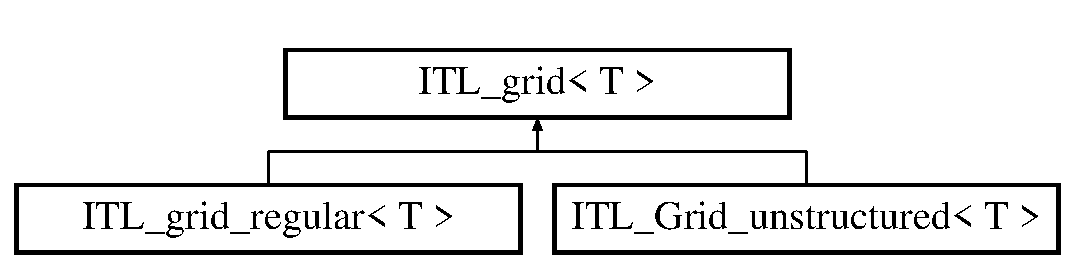
\includegraphics[height=2cm]{classITL__grid}
\end{center}
\end{figure}
\subsection*{Public Member Functions}
\begin{DoxyCompactItemize}
\item 
\hyperlink{classITL__grid_a8d06a30e48680ef7c7bd1a86f5008fa4}{ITL\_\-grid} ()
\begin{DoxyCompactList}\small\item\em Default constructor. \item\end{DoxyCompactList}\item 
\hyperlink{classITL__grid_a761ce2ffcfecbebac0abf6abd09c086c}{ITL\_\-grid} (int ndim)
\begin{DoxyCompactList}\small\item\em Constructor. \item\end{DoxyCompactList}\item 
virtual void \hyperlink{classITL__grid_a1df10dfdfddabe79e089aba810eccd8f}{setBounds} ()
\begin{DoxyCompactList}\small\item\em Pure virtual function. \item\end{DoxyCompactList}\item 
virtual void \hyperlink{classITL__grid_a808e49a6b0fe44a13f80df372146ce13}{setBounds} (float $\ast$l, float $\ast$h)
\begin{DoxyCompactList}\small\item\em Pure virtual function for setting the bounds of a grid with no ghost layers. \item\end{DoxyCompactList}\item 
virtual void \hyperlink{classITL__grid_adf6baf011a2d80f49a7e6007bcd190c7}{setBounds} (float $\ast$l, float $\ast$h, int $\ast$lPad, int $\ast$hPad, int neighborhoodsize)
\begin{DoxyCompactList}\small\item\em Pure virtual function for setting the bounds of a grid with ghost layers. \item\end{DoxyCompactList}\item 
virtual void \hyperlink{classITL__grid_aacc7102ddeec002827256c267b7eac38}{setBounds} (float $\ast$l, float $\ast$h, int $\ast$lPad, int $\ast$hPad, int $\ast$neighborhoodsizearray)
\item 
virtual int \hyperlink{classITL__grid_a2a1731cce0351121768b5a104e601057}{convert3DIndex} (int x, int y, int z)
\begin{DoxyCompactList}\small\item\em Pure virtual function for 3D spatial index to 1D array index conversion. \item\end{DoxyCompactList}\item 
virtual int \hyperlink{classITL__grid_ab43a701a19db72eafd919763f9092a74}{convert3DTimeVaryingIndex} (int x, int y, int z, int t)
\begin{DoxyCompactList}\small\item\em Pure virtual function for 3D+T spatial index to 1D array index conversion. \item\end{DoxyCompactList}\item 
virtual \hyperlink{classITL__grid_a44d1b2ed1e6e15cbf4067468b7b9fa96}{$\sim$ITL\_\-grid} ()
\begin{DoxyCompactList}\small\item\em Destructor. \item\end{DoxyCompactList}\end{DoxyCompactItemize}
\subsection*{Public Attributes}
\begin{DoxyCompactItemize}
\item 
int \hyperlink{classITL__grid_a81b6e8bd7659d7ffaafe0990351a5d22}{nDim}
\begin{DoxyCompactList}\small\item\em Number of dimensions. \item\end{DoxyCompactList}\item 
int $\ast$ \hyperlink{classITL__grid_a90ea972d6b2a9ce6e895bde21943e75d}{dim}
\begin{DoxyCompactList}\small\item\em Array for length of each dimension. \item\end{DoxyCompactList}\item 
int $\ast$ \hyperlink{classITL__grid_aa5c2e652215db2cbba916fdaab3e0bfb}{dimWithPad}
\begin{DoxyCompactList}\small\item\em Array for length of each dimension along with ghost layers (if any). \item\end{DoxyCompactList}\item 
int \hyperlink{classITL__grid_a21d38f7628465b0638ebd60f0fa11e7d}{nVertices}
\begin{DoxyCompactList}\small\item\em Number of vertices in Cartesian space. \item\end{DoxyCompactList}\item 
int \hyperlink{classITL__grid_a152743e564ed5b265c62c8462507e033}{nVerticesWithPad}
\begin{DoxyCompactList}\small\item\em Number of vertices along with ghost layers (if any) in Cartesian space. \item\end{DoxyCompactList}\item 
float $\ast$ \hyperlink{classITL__grid_abdab084ddf12b7bf745a4b76201757bf}{low}
\begin{DoxyCompactList}\small\item\em Lower bound of field in continuous Cartesian space. \item\end{DoxyCompactList}\item 
float $\ast$ \hyperlink{classITL__grid_a14b5be78196bb74d85cf3751a2b32b47}{high}
\begin{DoxyCompactList}\small\item\em Upper bound of field in continuous Cartesian space. \item\end{DoxyCompactList}\item 
int $\ast$ \hyperlink{classITL__grid_a3780830b49b613a702233bf4b9ccc467}{lowInt}
\begin{DoxyCompactList}\small\item\em Lower bound of field in discrete Cartesian space (nearest grid vertex containing the lower bound). \item\end{DoxyCompactList}\item 
int $\ast$ \hyperlink{classITL__grid_a60b5b9c9b8586ed362a09ba46dc6a158}{highInt}
\begin{DoxyCompactList}\small\item\em Upper bound of field in discrete Cartesian space (nearest grid vertex containing the upper bound). \item\end{DoxyCompactList}\item 
int $\ast$ \hyperlink{classITL__grid_a14f44c2a00f16d0c35a2cfbb72f61423}{lowIntWithPad}
\begin{DoxyCompactList}\small\item\em Lower bound of field in discrete Cartesian space along with ghost layers (if any). \item\end{DoxyCompactList}\item 
int $\ast$ \hyperlink{classITL__grid_ab9793b1da79d6926cc0d739f3da266c0}{highIntWithPad}
\begin{DoxyCompactList}\small\item\em Upper bound of field in discrete Cartesian space along with ghost layers (if any). \item\end{DoxyCompactList}\item 
int \hyperlink{classITL__grid_ace636892759ad4345c5f7725506ab329}{neighborhoodSize}
\begin{DoxyCompactList}\small\item\em Neighborhood length for each point. \item\end{DoxyCompactList}\item 
int $\ast$ \hyperlink{classITL__grid_a1d7b33b487dbe224fa10f11a23ee9f26}{lowPad}
\begin{DoxyCompactList}\small\item\em Span of ghost layers beyond lower end. \item\end{DoxyCompactList}\item 
int $\ast$ \hyperlink{classITL__grid_ac0d5d2e030b31036112cdcb3204d91ed}{highPad}
\begin{DoxyCompactList}\small\item\em Span of ghost layers beyond upper end. \item\end{DoxyCompactList}\item 
int $\ast$ \hyperlink{classITL__grid_a7f48b658a2978a050163c31bdce38524}{neighborhoodSizeArray}
\end{DoxyCompactItemize}


\subsection{Detailed Description}
\subsubsection*{template$<$class T$>$ class ITL\_\-grid$<$ T $>$}

Grid base class. A generic class for grid which contains information about spatial arrangement of field data points in a Cartesian space. Created on: Nov 17, 2010. \begin{DoxyAuthor}{Author}
Abon 

Teng-\/Yok 
\end{DoxyAuthor}


Definition at line 14 of file ITL\_\-grid.h.



\subsection{Constructor \& Destructor Documentation}
\hypertarget{classITL__grid_a8d06a30e48680ef7c7bd1a86f5008fa4}{
\index{ITL\_\-grid@{ITL\_\-grid}!ITL\_\-grid@{ITL\_\-grid}}
\index{ITL\_\-grid@{ITL\_\-grid}!ITL_grid@{ITL\_\-grid}}
\subsubsection[{ITL\_\-grid}]{\setlength{\rightskip}{0pt plus 5cm}template$<$class T$>$ {\bf ITL\_\-grid}$<$ T $>$::{\bf ITL\_\-grid} ()\hspace{0.3cm}{\ttfamily  \mbox{[}inline\mbox{]}}}}
\label{classITL__grid_a8d06a30e48680ef7c7bd1a86f5008fa4}


Default constructor. 



Definition at line 40 of file ITL\_\-grid.h.

\hypertarget{classITL__grid_a761ce2ffcfecbebac0abf6abd09c086c}{
\index{ITL\_\-grid@{ITL\_\-grid}!ITL\_\-grid@{ITL\_\-grid}}
\index{ITL\_\-grid@{ITL\_\-grid}!ITL_grid@{ITL\_\-grid}}
\subsubsection[{ITL\_\-grid}]{\setlength{\rightskip}{0pt plus 5cm}template$<$class T$>$ {\bf ITL\_\-grid}$<$ T $>$::{\bf ITL\_\-grid} (int {\em ndim})\hspace{0.3cm}{\ttfamily  \mbox{[}inline\mbox{]}}}}
\label{classITL__grid_a761ce2ffcfecbebac0abf6abd09c086c}


Constructor. 


\begin{DoxyParams}{Parameters}
\item[{\em ndim}]Dimensionality of the field. \end{DoxyParams}


Definition at line 46 of file ITL\_\-grid.h.

\hypertarget{classITL__grid_a44d1b2ed1e6e15cbf4067468b7b9fa96}{
\index{ITL\_\-grid@{ITL\_\-grid}!$\sim$ITL\_\-grid@{$\sim$ITL\_\-grid}}
\index{$\sim$ITL\_\-grid@{$\sim$ITL\_\-grid}!ITL_grid@{ITL\_\-grid}}
\subsubsection[{$\sim$ITL\_\-grid}]{\setlength{\rightskip}{0pt plus 5cm}template$<$class T$>$ virtual {\bf ITL\_\-grid}$<$ T $>$::$\sim${\bf ITL\_\-grid} ()\hspace{0.3cm}{\ttfamily  \mbox{[}inline, virtual\mbox{]}}}}
\label{classITL__grid_a44d1b2ed1e6e15cbf4067468b7b9fa96}


Destructor. 



Definition at line 76 of file ITL\_\-grid.h.



\subsection{Member Function Documentation}
\hypertarget{classITL__grid_a2a1731cce0351121768b5a104e601057}{
\index{ITL\_\-grid@{ITL\_\-grid}!convert3DIndex@{convert3DIndex}}
\index{convert3DIndex@{convert3DIndex}!ITL_grid@{ITL\_\-grid}}
\subsubsection[{convert3DIndex}]{\setlength{\rightskip}{0pt plus 5cm}template$<$class T$>$ virtual int {\bf ITL\_\-grid}$<$ T $>$::convert3DIndex (int {\em x}, \/  int {\em y}, \/  int {\em z})\hspace{0.3cm}{\ttfamily  \mbox{[}inline, virtual\mbox{]}}}}
\label{classITL__grid_a2a1731cce0351121768b5a104e601057}


Pure virtual function for 3D spatial index to 1D array index conversion. 



Reimplemented in \hyperlink{classITL__grid__regular_a9561a0c36a74216eef9685d5f3369f7a}{ITL\_\-grid\_\-regular$<$ T $>$}.



Definition at line 68 of file ITL\_\-grid.h.

\hypertarget{classITL__grid_ab43a701a19db72eafd919763f9092a74}{
\index{ITL\_\-grid@{ITL\_\-grid}!convert3DTimeVaryingIndex@{convert3DTimeVaryingIndex}}
\index{convert3DTimeVaryingIndex@{convert3DTimeVaryingIndex}!ITL_grid@{ITL\_\-grid}}
\subsubsection[{convert3DTimeVaryingIndex}]{\setlength{\rightskip}{0pt plus 5cm}template$<$class T$>$ virtual int {\bf ITL\_\-grid}$<$ T $>$::convert3DTimeVaryingIndex (int {\em x}, \/  int {\em y}, \/  int {\em z}, \/  int {\em t})\hspace{0.3cm}{\ttfamily  \mbox{[}inline, virtual\mbox{]}}}}
\label{classITL__grid_ab43a701a19db72eafd919763f9092a74}


Pure virtual function for 3D+T spatial index to 1D array index conversion. 



Definition at line 72 of file ITL\_\-grid.h.

\hypertarget{classITL__grid_aacc7102ddeec002827256c267b7eac38}{
\index{ITL\_\-grid@{ITL\_\-grid}!setBounds@{setBounds}}
\index{setBounds@{setBounds}!ITL_grid@{ITL\_\-grid}}
\subsubsection[{setBounds}]{\setlength{\rightskip}{0pt plus 5cm}template$<$class T$>$ virtual void {\bf ITL\_\-grid}$<$ T $>$::setBounds (float $\ast$ {\em l}, \/  float $\ast$ {\em h}, \/  int $\ast$ {\em lPad}, \/  int $\ast$ {\em hPad}, \/  int $\ast$ {\em neighborhoodsizearray})\hspace{0.3cm}{\ttfamily  \mbox{[}inline, virtual\mbox{]}}}}
\label{classITL__grid_aacc7102ddeec002827256c267b7eac38}


Reimplemented in \hyperlink{classITL__grid__regular_a324d135ffc7a8e3dab70933f036c7e5a}{ITL\_\-grid\_\-regular$<$ T $>$}.



Definition at line 64 of file ITL\_\-grid.h.

\hypertarget{classITL__grid_adf6baf011a2d80f49a7e6007bcd190c7}{
\index{ITL\_\-grid@{ITL\_\-grid}!setBounds@{setBounds}}
\index{setBounds@{setBounds}!ITL_grid@{ITL\_\-grid}}
\subsubsection[{setBounds}]{\setlength{\rightskip}{0pt plus 5cm}template$<$class T$>$ virtual void {\bf ITL\_\-grid}$<$ T $>$::setBounds (float $\ast$ {\em l}, \/  float $\ast$ {\em h}, \/  int $\ast$ {\em lPad}, \/  int $\ast$ {\em hPad}, \/  int {\em neighborhoodsize})\hspace{0.3cm}{\ttfamily  \mbox{[}inline, virtual\mbox{]}}}}
\label{classITL__grid_adf6baf011a2d80f49a7e6007bcd190c7}


Pure virtual function for setting the bounds of a grid with ghost layers. 



Reimplemented in \hyperlink{classITL__grid__regular_ac64d7fd91b4330f961979a6d7127d9f6}{ITL\_\-grid\_\-regular$<$ T $>$}.



Definition at line 63 of file ITL\_\-grid.h.

\hypertarget{classITL__grid_a808e49a6b0fe44a13f80df372146ce13}{
\index{ITL\_\-grid@{ITL\_\-grid}!setBounds@{setBounds}}
\index{setBounds@{setBounds}!ITL_grid@{ITL\_\-grid}}
\subsubsection[{setBounds}]{\setlength{\rightskip}{0pt plus 5cm}template$<$class T$>$ virtual void {\bf ITL\_\-grid}$<$ T $>$::setBounds (float $\ast$ {\em l}, \/  float $\ast$ {\em h})\hspace{0.3cm}{\ttfamily  \mbox{[}inline, virtual\mbox{]}}}}
\label{classITL__grid_a808e49a6b0fe44a13f80df372146ce13}


Pure virtual function for setting the bounds of a grid with no ghost layers. 



Reimplemented in \hyperlink{classITL__grid__regular_aae7fcdd0c0da2df91cbe6b658a7ce43c}{ITL\_\-grid\_\-regular$<$ T $>$}.



Definition at line 59 of file ITL\_\-grid.h.

\hypertarget{classITL__grid_a1df10dfdfddabe79e089aba810eccd8f}{
\index{ITL\_\-grid@{ITL\_\-grid}!setBounds@{setBounds}}
\index{setBounds@{setBounds}!ITL_grid@{ITL\_\-grid}}
\subsubsection[{setBounds}]{\setlength{\rightskip}{0pt plus 5cm}template$<$class T$>$ virtual void {\bf ITL\_\-grid}$<$ T $>$::setBounds ()\hspace{0.3cm}{\ttfamily  \mbox{[}inline, virtual\mbox{]}}}}
\label{classITL__grid_a1df10dfdfddabe79e089aba810eccd8f}


Pure virtual function. 



Definition at line 55 of file ITL\_\-grid.h.



\subsection{Member Data Documentation}
\hypertarget{classITL__grid_a90ea972d6b2a9ce6e895bde21943e75d}{
\index{ITL\_\-grid@{ITL\_\-grid}!dim@{dim}}
\index{dim@{dim}!ITL_grid@{ITL\_\-grid}}
\subsubsection[{dim}]{\setlength{\rightskip}{0pt plus 5cm}template$<$class T$>$ int$\ast$ {\bf ITL\_\-grid}$<$ T $>$::{\bf dim}}}
\label{classITL__grid_a90ea972d6b2a9ce6e895bde21943e75d}


Array for length of each dimension. 



Definition at line 19 of file ITL\_\-grid.h.

\hypertarget{classITL__grid_aa5c2e652215db2cbba916fdaab3e0bfb}{
\index{ITL\_\-grid@{ITL\_\-grid}!dimWithPad@{dimWithPad}}
\index{dimWithPad@{dimWithPad}!ITL_grid@{ITL\_\-grid}}
\subsubsection[{dimWithPad}]{\setlength{\rightskip}{0pt plus 5cm}template$<$class T$>$ int$\ast$ {\bf ITL\_\-grid}$<$ T $>$::{\bf dimWithPad}}}
\label{classITL__grid_aa5c2e652215db2cbba916fdaab3e0bfb}


Array for length of each dimension along with ghost layers (if any). 



Definition at line 20 of file ITL\_\-grid.h.

\hypertarget{classITL__grid_a14b5be78196bb74d85cf3751a2b32b47}{
\index{ITL\_\-grid@{ITL\_\-grid}!high@{high}}
\index{high@{high}!ITL_grid@{ITL\_\-grid}}
\subsubsection[{high}]{\setlength{\rightskip}{0pt plus 5cm}template$<$class T$>$ float$\ast$ {\bf ITL\_\-grid}$<$ T $>$::{\bf high}}}
\label{classITL__grid_a14b5be78196bb74d85cf3751a2b32b47}


Upper bound of field in continuous Cartesian space. 

Limit may not coincide with a grid vertex 

Definition at line 24 of file ITL\_\-grid.h.

\hypertarget{classITL__grid_a60b5b9c9b8586ed362a09ba46dc6a158}{
\index{ITL\_\-grid@{ITL\_\-grid}!highInt@{highInt}}
\index{highInt@{highInt}!ITL_grid@{ITL\_\-grid}}
\subsubsection[{highInt}]{\setlength{\rightskip}{0pt plus 5cm}template$<$class T$>$ int$\ast$ {\bf ITL\_\-grid}$<$ T $>$::{\bf highInt}}}
\label{classITL__grid_a60b5b9c9b8586ed362a09ba46dc6a158}


Upper bound of field in discrete Cartesian space (nearest grid vertex containing the upper bound). 



Definition at line 26 of file ITL\_\-grid.h.

\hypertarget{classITL__grid_ab9793b1da79d6926cc0d739f3da266c0}{
\index{ITL\_\-grid@{ITL\_\-grid}!highIntWithPad@{highIntWithPad}}
\index{highIntWithPad@{highIntWithPad}!ITL_grid@{ITL\_\-grid}}
\subsubsection[{highIntWithPad}]{\setlength{\rightskip}{0pt plus 5cm}template$<$class T$>$ int$\ast$ {\bf ITL\_\-grid}$<$ T $>$::{\bf highIntWithPad}}}
\label{classITL__grid_ab9793b1da79d6926cc0d739f3da266c0}


Upper bound of field in discrete Cartesian space along with ghost layers (if any). 



Definition at line 28 of file ITL\_\-grid.h.

\hypertarget{classITL__grid_ac0d5d2e030b31036112cdcb3204d91ed}{
\index{ITL\_\-grid@{ITL\_\-grid}!highPad@{highPad}}
\index{highPad@{highPad}!ITL_grid@{ITL\_\-grid}}
\subsubsection[{highPad}]{\setlength{\rightskip}{0pt plus 5cm}template$<$class T$>$ int$\ast$ {\bf ITL\_\-grid}$<$ T $>$::{\bf highPad}}}
\label{classITL__grid_ac0d5d2e030b31036112cdcb3204d91ed}


Span of ghost layers beyond upper end. 



Definition at line 32 of file ITL\_\-grid.h.

\hypertarget{classITL__grid_abdab084ddf12b7bf745a4b76201757bf}{
\index{ITL\_\-grid@{ITL\_\-grid}!low@{low}}
\index{low@{low}!ITL_grid@{ITL\_\-grid}}
\subsubsection[{low}]{\setlength{\rightskip}{0pt plus 5cm}template$<$class T$>$ float$\ast$ {\bf ITL\_\-grid}$<$ T $>$::{\bf low}}}
\label{classITL__grid_abdab084ddf12b7bf745a4b76201757bf}


Lower bound of field in continuous Cartesian space. 

Limit may not coincide with a grid vertex 

Definition at line 23 of file ITL\_\-grid.h.

\hypertarget{classITL__grid_a3780830b49b613a702233bf4b9ccc467}{
\index{ITL\_\-grid@{ITL\_\-grid}!lowInt@{lowInt}}
\index{lowInt@{lowInt}!ITL_grid@{ITL\_\-grid}}
\subsubsection[{lowInt}]{\setlength{\rightskip}{0pt plus 5cm}template$<$class T$>$ int$\ast$ {\bf ITL\_\-grid}$<$ T $>$::{\bf lowInt}}}
\label{classITL__grid_a3780830b49b613a702233bf4b9ccc467}


Lower bound of field in discrete Cartesian space (nearest grid vertex containing the lower bound). 



Definition at line 25 of file ITL\_\-grid.h.

\hypertarget{classITL__grid_a14f44c2a00f16d0c35a2cfbb72f61423}{
\index{ITL\_\-grid@{ITL\_\-grid}!lowIntWithPad@{lowIntWithPad}}
\index{lowIntWithPad@{lowIntWithPad}!ITL_grid@{ITL\_\-grid}}
\subsubsection[{lowIntWithPad}]{\setlength{\rightskip}{0pt plus 5cm}template$<$class T$>$ int$\ast$ {\bf ITL\_\-grid}$<$ T $>$::{\bf lowIntWithPad}}}
\label{classITL__grid_a14f44c2a00f16d0c35a2cfbb72f61423}


Lower bound of field in discrete Cartesian space along with ghost layers (if any). 



Definition at line 27 of file ITL\_\-grid.h.

\hypertarget{classITL__grid_a1d7b33b487dbe224fa10f11a23ee9f26}{
\index{ITL\_\-grid@{ITL\_\-grid}!lowPad@{lowPad}}
\index{lowPad@{lowPad}!ITL_grid@{ITL\_\-grid}}
\subsubsection[{lowPad}]{\setlength{\rightskip}{0pt plus 5cm}template$<$class T$>$ int$\ast$ {\bf ITL\_\-grid}$<$ T $>$::{\bf lowPad}}}
\label{classITL__grid_a1d7b33b487dbe224fa10f11a23ee9f26}


Span of ghost layers beyond lower end. 



Definition at line 31 of file ITL\_\-grid.h.

\hypertarget{classITL__grid_a81b6e8bd7659d7ffaafe0990351a5d22}{
\index{ITL\_\-grid@{ITL\_\-grid}!nDim@{nDim}}
\index{nDim@{nDim}!ITL_grid@{ITL\_\-grid}}
\subsubsection[{nDim}]{\setlength{\rightskip}{0pt plus 5cm}template$<$class T$>$ int {\bf ITL\_\-grid}$<$ T $>$::{\bf nDim}}}
\label{classITL__grid_a81b6e8bd7659d7ffaafe0990351a5d22}


Number of dimensions. 



Definition at line 18 of file ITL\_\-grid.h.

\hypertarget{classITL__grid_ace636892759ad4345c5f7725506ab329}{
\index{ITL\_\-grid@{ITL\_\-grid}!neighborhoodSize@{neighborhoodSize}}
\index{neighborhoodSize@{neighborhoodSize}!ITL_grid@{ITL\_\-grid}}
\subsubsection[{neighborhoodSize}]{\setlength{\rightskip}{0pt plus 5cm}template$<$class T$>$ int {\bf ITL\_\-grid}$<$ T $>$::{\bf neighborhoodSize}}}
\label{classITL__grid_ace636892759ad4345c5f7725506ab329}


Neighborhood length for each point. 

Helps to determine span of ghost layers 

Definition at line 30 of file ITL\_\-grid.h.

\hypertarget{classITL__grid_a7f48b658a2978a050163c31bdce38524}{
\index{ITL\_\-grid@{ITL\_\-grid}!neighborhoodSizeArray@{neighborhoodSizeArray}}
\index{neighborhoodSizeArray@{neighborhoodSizeArray}!ITL_grid@{ITL\_\-grid}}
\subsubsection[{neighborhoodSizeArray}]{\setlength{\rightskip}{0pt plus 5cm}template$<$class T$>$ int$\ast$ {\bf ITL\_\-grid}$<$ T $>$::{\bf neighborhoodSizeArray}}}
\label{classITL__grid_a7f48b658a2978a050163c31bdce38524}


Definition at line 33 of file ITL\_\-grid.h.

\hypertarget{classITL__grid_a21d38f7628465b0638ebd60f0fa11e7d}{
\index{ITL\_\-grid@{ITL\_\-grid}!nVertices@{nVertices}}
\index{nVertices@{nVertices}!ITL_grid@{ITL\_\-grid}}
\subsubsection[{nVertices}]{\setlength{\rightskip}{0pt plus 5cm}template$<$class T$>$ int {\bf ITL\_\-grid}$<$ T $>$::{\bf nVertices}}}
\label{classITL__grid_a21d38f7628465b0638ebd60f0fa11e7d}


Number of vertices in Cartesian space. 



Definition at line 21 of file ITL\_\-grid.h.

\hypertarget{classITL__grid_a152743e564ed5b265c62c8462507e033}{
\index{ITL\_\-grid@{ITL\_\-grid}!nVerticesWithPad@{nVerticesWithPad}}
\index{nVerticesWithPad@{nVerticesWithPad}!ITL_grid@{ITL\_\-grid}}
\subsubsection[{nVerticesWithPad}]{\setlength{\rightskip}{0pt plus 5cm}template$<$class T$>$ int {\bf ITL\_\-grid}$<$ T $>$::{\bf nVerticesWithPad}}}
\label{classITL__grid_a152743e564ed5b265c62c8462507e033}


Number of vertices along with ghost layers (if any) in Cartesian space. 



Definition at line 22 of file ITL\_\-grid.h.



The documentation for this class was generated from the following file:\begin{DoxyCompactItemize}
\item 
/home/abon/Code/workspace\_\-unix/ITL\_\-repo/include/\hyperlink{ITL__grid_8h}{ITL\_\-grid.h}\end{DoxyCompactItemize}

\hypertarget{classITL__grid__regular}{
\section{ITL\_\-grid\_\-regular$<$ T $>$ Class Template Reference}
\label{classITL__grid__regular}\index{ITL\_\-grid\_\-regular@{ITL\_\-grid\_\-regular}}
}


Regular grid inherited from \hyperlink{classITL__grid}{ITL\_\-grid}.  




{\ttfamily \#include $<$ITL\_\-grid\_\-regular.h$>$}

Inheritance diagram for ITL\_\-grid\_\-regular$<$ T $>$:\begin{figure}[H]
\begin{center}
\leavevmode
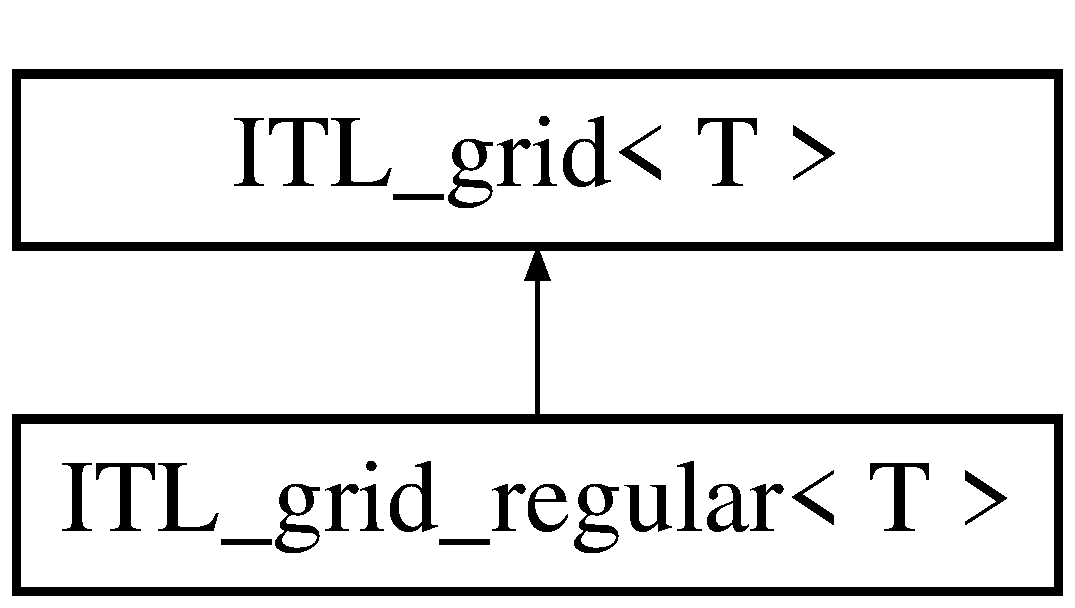
\includegraphics[height=2cm]{classITL__grid__regular}
\end{center}
\end{figure}
\subsection*{Public Member Functions}
\begin{DoxyCompactItemize}
\item 
\hyperlink{classITL__grid__regular_a6fc8f7b939590292ec89bf0e69dd3329}{ITL\_\-grid\_\-regular} (int ndim)
\begin{DoxyCompactList}\small\item\em Constructor. \item\end{DoxyCompactList}\item 
void \hyperlink{classITL__grid__regular_aae7fcdd0c0da2df91cbe6b658a7ce43c}{setBounds} (float $\ast$l, float $\ast$h)
\begin{DoxyCompactList}\small\item\em Function for setting the bounds of a grid with no ghost layers. \item\end{DoxyCompactList}\item 
void \hyperlink{classITL__grid__regular_ac64d7fd91b4330f961979a6d7127d9f6}{setBounds} (float $\ast$l, float $\ast$h, int $\ast$lPad, int $\ast$hPad, int neighborhoodsize)
\begin{DoxyCompactList}\small\item\em Function for setting the bounds of a grid with ghost layers. \item\end{DoxyCompactList}\item 
void \hyperlink{classITL__grid__regular_a324d135ffc7a8e3dab70933f036c7e5a}{setBounds} (float $\ast$l, float $\ast$h, int $\ast$lPad, int $\ast$hPad, int $\ast$neighborhoodsizearray)
\item 
int \hyperlink{classITL__grid__regular_a9561a0c36a74216eef9685d5f3369f7a}{convert3DIndex} (int x, int y, int z)
\begin{DoxyCompactList}\small\item\em Function for 3D spatial index to 1D array index conversion. \item\end{DoxyCompactList}\item 
int \hyperlink{classITL__grid__regular_a6172df2903ce28b33f158ccaa3741774}{convertTimeVarying3DIndex} (int x, int y, int z, int t)
\begin{DoxyCompactList}\small\item\em Function for 3D+T spatial index to 1D array index conversion. \item\end{DoxyCompactList}\item 
\hyperlink{classITL__grid__regular_a360a8aba9edd80a56d2f0020c89d1287}{$\sim$ITL\_\-grid\_\-regular} ()
\begin{DoxyCompactList}\small\item\em Destructor. \item\end{DoxyCompactList}\end{DoxyCompactItemize}


\subsection{Detailed Description}
\subsubsection*{template$<$class T$>$ class ITL\_\-grid\_\-regular$<$ T $>$}

Regular grid inherited from \hyperlink{classITL__grid}{ITL\_\-grid}. A class which contains information about spatial arrangement of field data points regularly arranged in a Cartesian space. Created on: Dec 9, 2010 \begin{DoxyAuthor}{Author}
Abon 

Teng-\/Yok 
\end{DoxyAuthor}


Definition at line 16 of file ITL\_\-grid\_\-regular.h.



\subsection{Constructor \& Destructor Documentation}
\hypertarget{classITL__grid__regular_a6fc8f7b939590292ec89bf0e69dd3329}{
\index{ITL\_\-grid\_\-regular@{ITL\_\-grid\_\-regular}!ITL\_\-grid\_\-regular@{ITL\_\-grid\_\-regular}}
\index{ITL\_\-grid\_\-regular@{ITL\_\-grid\_\-regular}!ITL_grid_regular@{ITL\_\-grid\_\-regular}}
\subsubsection[{ITL\_\-grid\_\-regular}]{\setlength{\rightskip}{0pt plus 5cm}template$<$class T$>$ {\bf ITL\_\-grid\_\-regular}$<$ T $>$::{\bf ITL\_\-grid\_\-regular} (int {\em ndim})\hspace{0.3cm}{\ttfamily  \mbox{[}inline\mbox{]}}}}
\label{classITL__grid__regular_a6fc8f7b939590292ec89bf0e69dd3329}


Constructor. 


\begin{DoxyParams}{Parameters}
\item[{\em ndim}]Dimensionality of the field. \end{DoxyParams}


Definition at line 24 of file ITL\_\-grid\_\-regular.h.

\hypertarget{classITL__grid__regular_a360a8aba9edd80a56d2f0020c89d1287}{
\index{ITL\_\-grid\_\-regular@{ITL\_\-grid\_\-regular}!$\sim$ITL\_\-grid\_\-regular@{$\sim$ITL\_\-grid\_\-regular}}
\index{$\sim$ITL\_\-grid\_\-regular@{$\sim$ITL\_\-grid\_\-regular}!ITL_grid_regular@{ITL\_\-grid\_\-regular}}
\subsubsection[{$\sim$ITL\_\-grid\_\-regular}]{\setlength{\rightskip}{0pt plus 5cm}template$<$class T$>$ {\bf ITL\_\-grid\_\-regular}$<$ T $>$::$\sim${\bf ITL\_\-grid\_\-regular} ()\hspace{0.3cm}{\ttfamily  \mbox{[}inline\mbox{]}}}}
\label{classITL__grid__regular_a360a8aba9edd80a56d2f0020c89d1287}


Destructor. 



Definition at line 254 of file ITL\_\-grid\_\-regular.h.



\subsection{Member Function Documentation}
\hypertarget{classITL__grid__regular_a9561a0c36a74216eef9685d5f3369f7a}{
\index{ITL\_\-grid\_\-regular@{ITL\_\-grid\_\-regular}!convert3DIndex@{convert3DIndex}}
\index{convert3DIndex@{convert3DIndex}!ITL_grid_regular@{ITL\_\-grid\_\-regular}}
\subsubsection[{convert3DIndex}]{\setlength{\rightskip}{0pt plus 5cm}template$<$class T$>$ int {\bf ITL\_\-grid\_\-regular}$<$ T $>$::convert3DIndex (int {\em x}, \/  int {\em y}, \/  int {\em z})\hspace{0.3cm}{\ttfamily  \mbox{[}inline, virtual\mbox{]}}}}
\label{classITL__grid__regular_a9561a0c36a74216eef9685d5f3369f7a}


Function for 3D spatial index to 1D array index conversion. 


\begin{DoxyParams}{Parameters}
\item[{\em x}]x-\/coordinate of the spatial point. \item[{\em y}]y-\/coordinate of the spatial point. \item[{\em z}]z-\/coordinate of the spatial point. \end{DoxyParams}


Reimplemented from \hyperlink{classITL__grid_a2a1731cce0351121768b5a104e601057}{ITL\_\-grid$<$ T $>$}.



Definition at line 234 of file ITL\_\-grid\_\-regular.h.

\hypertarget{classITL__grid__regular_a6172df2903ce28b33f158ccaa3741774}{
\index{ITL\_\-grid\_\-regular@{ITL\_\-grid\_\-regular}!convertTimeVarying3DIndex@{convertTimeVarying3DIndex}}
\index{convertTimeVarying3DIndex@{convertTimeVarying3DIndex}!ITL_grid_regular@{ITL\_\-grid\_\-regular}}
\subsubsection[{convertTimeVarying3DIndex}]{\setlength{\rightskip}{0pt plus 5cm}template$<$class T$>$ int {\bf ITL\_\-grid\_\-regular}$<$ T $>$::convertTimeVarying3DIndex (int {\em x}, \/  int {\em y}, \/  int {\em z}, \/  int {\em t})\hspace{0.3cm}{\ttfamily  \mbox{[}inline\mbox{]}}}}
\label{classITL__grid__regular_a6172df2903ce28b33f158ccaa3741774}


Function for 3D+T spatial index to 1D array index conversion. 


\begin{DoxyParams}{Parameters}
\item[{\em x}]x-\/coordinate of the spatial point. \item[{\em y}]y-\/coordinate of the spatial point. \item[{\em z}]z-\/coordinate of the spatial point. \item[{\em t}]t-\/coordinate of the spatial point. \end{DoxyParams}


Definition at line 246 of file ITL\_\-grid\_\-regular.h.

\hypertarget{classITL__grid__regular_a324d135ffc7a8e3dab70933f036c7e5a}{
\index{ITL\_\-grid\_\-regular@{ITL\_\-grid\_\-regular}!setBounds@{setBounds}}
\index{setBounds@{setBounds}!ITL_grid_regular@{ITL\_\-grid\_\-regular}}
\subsubsection[{setBounds}]{\setlength{\rightskip}{0pt plus 5cm}template$<$class T$>$ void {\bf ITL\_\-grid\_\-regular}$<$ T $>$::setBounds (float $\ast$ {\em l}, \/  float $\ast$ {\em h}, \/  int $\ast$ {\em lPad}, \/  int $\ast$ {\em hPad}, \/  int $\ast$ {\em neighborhoodsizearray})\hspace{0.3cm}{\ttfamily  \mbox{[}inline, virtual\mbox{]}}}}
\label{classITL__grid__regular_a324d135ffc7a8e3dab70933f036c7e5a}


Reimplemented from \hyperlink{classITL__grid_aacc7102ddeec002827256c267b7eac38}{ITL\_\-grid$<$ T $>$}.



Definition at line 164 of file ITL\_\-grid\_\-regular.h.

\hypertarget{classITL__grid__regular_ac64d7fd91b4330f961979a6d7127d9f6}{
\index{ITL\_\-grid\_\-regular@{ITL\_\-grid\_\-regular}!setBounds@{setBounds}}
\index{setBounds@{setBounds}!ITL_grid_regular@{ITL\_\-grid\_\-regular}}
\subsubsection[{setBounds}]{\setlength{\rightskip}{0pt plus 5cm}template$<$class T$>$ void {\bf ITL\_\-grid\_\-regular}$<$ T $>$::setBounds (float $\ast$ {\em l}, \/  float $\ast$ {\em h}, \/  int $\ast$ {\em lPad}, \/  int $\ast$ {\em hPad}, \/  int {\em neighborhoodsize})\hspace{0.3cm}{\ttfamily  \mbox{[}inline, virtual\mbox{]}}}}
\label{classITL__grid__regular_ac64d7fd91b4330f961979a6d7127d9f6}


Function for setting the bounds of a grid with ghost layers. 


\begin{DoxyParams}{Parameters}
\item[{\em l}]Pointer to array containing lower grid bounds in continuous space along each dimension. \item[{\em h}]Pointer to array containing upper grid bounds in continuous space along each dimension. \item[{\em lPad}]Pointer to array containing ghost layaer span along each dimension on the lower end. \item[{\em hPad}]Pointer to array containing ghost layaer span along each dimension on the upper end. \item[{\em neighborhoodsize}]Neighborhood length for each point. \end{DoxyParams}


Reimplemented from \hyperlink{classITL__grid_adf6baf011a2d80f49a7e6007bcd190c7}{ITL\_\-grid$<$ T $>$}.



Definition at line 103 of file ITL\_\-grid\_\-regular.h.

\hypertarget{classITL__grid__regular_aae7fcdd0c0da2df91cbe6b658a7ce43c}{
\index{ITL\_\-grid\_\-regular@{ITL\_\-grid\_\-regular}!setBounds@{setBounds}}
\index{setBounds@{setBounds}!ITL_grid_regular@{ITL\_\-grid\_\-regular}}
\subsubsection[{setBounds}]{\setlength{\rightskip}{0pt plus 5cm}template$<$class T$>$ void {\bf ITL\_\-grid\_\-regular}$<$ T $>$::setBounds (float $\ast$ {\em l}, \/  float $\ast$ {\em h})\hspace{0.3cm}{\ttfamily  \mbox{[}inline, virtual\mbox{]}}}}
\label{classITL__grid__regular_aae7fcdd0c0da2df91cbe6b658a7ce43c}


Function for setting the bounds of a grid with no ghost layers. 


\begin{DoxyParams}{Parameters}
\item[{\em l}]Pointer to array containing lower grid bounds in continuous space along each dimension. \item[{\em h}]Pointer to array containing upper grid bounds in continuous space along each dimension. \end{DoxyParams}


Reimplemented from \hyperlink{classITL__grid_a808e49a6b0fe44a13f80df372146ce13}{ITL\_\-grid$<$ T $>$}.



Definition at line 35 of file ITL\_\-grid\_\-regular.h.



The documentation for this class was generated from the following file:\begin{DoxyCompactItemize}
\item 
/home/abon/Code/workspace\_\-unix/ITL\_\-repo/include/\hyperlink{ITL__grid__regular_8h}{ITL\_\-grid\_\-regular.h}\end{DoxyCompactItemize}

\hypertarget{classITL__grid__tetrahedral}{
\section{ITL\_\-grid\_\-tetrahedral$<$ T $>$ Class Template Reference}
\label{classITL__grid__tetrahedral}\index{ITL\_\-grid\_\-tetrahedral@{ITL\_\-grid\_\-tetrahedral}}
}


Tetrahedral unstructured grid inherited from ITL\_\-grid\_\-unstructured.  




{\ttfamily \#include $<$ITL\_\-grid\_\-tetrahedral.h$>$}

\subsection*{Public Member Functions}
\begin{DoxyCompactItemize}
\item 
\hyperlink{classITL__grid__tetrahedral_a1687d1ed412ceb76d008a871eb038936}{ITL\_\-grid\_\-tetrahedral} ()
\begin{DoxyCompactList}\small\item\em Constructor. \item\end{DoxyCompactList}\end{DoxyCompactItemize}
\subsection*{Public Attributes}
\begin{DoxyCompactItemize}
\item 
int \hyperlink{classITL__grid__tetrahedral_a4f290e007f6b76fc039de3faf68276df}{nCell}
\item 
\hyperlink{classITL__tetrahedron}{ITL\_\-tetrahedron} $\ast$ \hyperlink{classITL__grid__tetrahedral_a4ce6a6ca28a0f7ba4c62e2a92eb6076e}{listOfCells}
\end{DoxyCompactItemize}


\subsection{Detailed Description}
\subsubsection*{template$<$class T$>$ class ITL\_\-grid\_\-tetrahedral$<$ T $>$}

Tetrahedral unstructured grid inherited from ITL\_\-grid\_\-unstructured. A class which contains information about spatial arrangement and connectivity of field data points arranged as a series of tetrahedra in a Cartesian space. We currently assume that the grid is 3-\/dimensional. Created on: Aptil 28, 2011 \begin{DoxyAuthor}{Author}
Abon 

Teng-\/Yok 
\end{DoxyAuthor}


Definition at line 19 of file ITL\_\-grid\_\-tetrahedral.h.



\subsection{Constructor \& Destructor Documentation}
\hypertarget{classITL__grid__tetrahedral_a1687d1ed412ceb76d008a871eb038936}{
\index{ITL\_\-grid\_\-tetrahedral@{ITL\_\-grid\_\-tetrahedral}!ITL\_\-grid\_\-tetrahedral@{ITL\_\-grid\_\-tetrahedral}}
\index{ITL\_\-grid\_\-tetrahedral@{ITL\_\-grid\_\-tetrahedral}!ITL_grid_tetrahedral@{ITL\_\-grid\_\-tetrahedral}}
\subsubsection[{ITL\_\-grid\_\-tetrahedral}]{\setlength{\rightskip}{0pt plus 5cm}template$<$class T $>$ {\bf ITL\_\-grid\_\-tetrahedral}$<$ T $>$::{\bf ITL\_\-grid\_\-tetrahedral} ()\hspace{0.3cm}{\ttfamily  \mbox{[}inline\mbox{]}}}}
\label{classITL__grid__tetrahedral_a1687d1ed412ceb76d008a871eb038936}


Constructor. 


\begin{DoxyParams}{Parameters}
\item[{\em ndim}]Dimensionality of the field. \end{DoxyParams}


Definition at line 29 of file ITL\_\-grid\_\-tetrahedral.h.



\subsection{Member Data Documentation}
\hypertarget{classITL__grid__tetrahedral_a4ce6a6ca28a0f7ba4c62e2a92eb6076e}{
\index{ITL\_\-grid\_\-tetrahedral@{ITL\_\-grid\_\-tetrahedral}!listOfCells@{listOfCells}}
\index{listOfCells@{listOfCells}!ITL_grid_tetrahedral@{ITL\_\-grid\_\-tetrahedral}}
\subsubsection[{listOfCells}]{\setlength{\rightskip}{0pt plus 5cm}template$<$class T $>$ {\bf ITL\_\-tetrahedron}$\ast$ {\bf ITL\_\-grid\_\-tetrahedral}$<$ T $>$::{\bf listOfCells}}}
\label{classITL__grid__tetrahedral_a4ce6a6ca28a0f7ba4c62e2a92eb6076e}


Definition at line 21 of file ITL\_\-grid\_\-tetrahedral.h.

\hypertarget{classITL__grid__tetrahedral_a4f290e007f6b76fc039de3faf68276df}{
\index{ITL\_\-grid\_\-tetrahedral@{ITL\_\-grid\_\-tetrahedral}!nCell@{nCell}}
\index{nCell@{nCell}!ITL_grid_tetrahedral@{ITL\_\-grid\_\-tetrahedral}}
\subsubsection[{nCell}]{\setlength{\rightskip}{0pt plus 5cm}template$<$class T $>$ int {\bf ITL\_\-grid\_\-tetrahedral}$<$ T $>$::{\bf nCell}}}
\label{classITL__grid__tetrahedral_a4f290e007f6b76fc039de3faf68276df}


Definition at line 20 of file ITL\_\-grid\_\-tetrahedral.h.



The documentation for this class was generated from the following file:\begin{DoxyCompactItemize}
\item 
/home/abon/Code/workspace\_\-unix/ITL\_\-repo/include/\hyperlink{ITL__grid__tetrahedral_8h}{ITL\_\-grid\_\-tetrahedral.h}\end{DoxyCompactItemize}

\hypertarget{classITL__Grid__unstructured}{
\section{ITL\_\-Grid\_\-unstructured$<$ T $>$ Class Template Reference}
\label{classITL__Grid__unstructured}\index{ITL\_\-Grid\_\-unstructured@{ITL\_\-Grid\_\-unstructured}}
}


Unstructured grid inherited from \hyperlink{classITL__grid}{ITL\_\-grid}.  




{\ttfamily \#include $<$ITL\_\-grid\_\-unstructured.h$>$}

Inheritance diagram for ITL\_\-Grid\_\-unstructured$<$ T $>$:\begin{figure}[H]
\begin{center}
\leavevmode
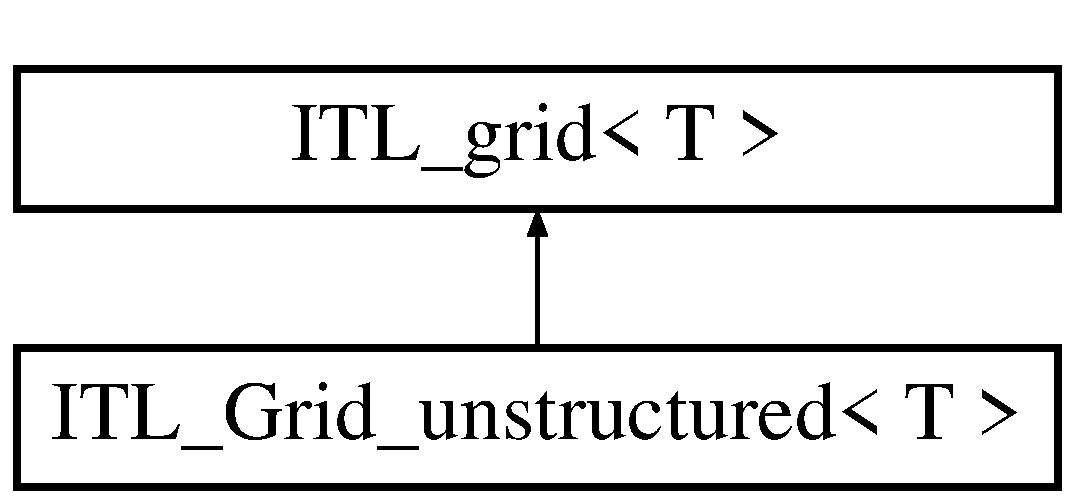
\includegraphics[height=2cm]{classITL__Grid__unstructured}
\end{center}
\end{figure}
\subsection*{Public Member Functions}
\begin{DoxyCompactItemize}
\item 
\hyperlink{classITL__Grid__unstructured_a05310e279796cc06c54ebe0035860889}{ITL\_\-grid\_\-unstructured} (int ndim)
\begin{DoxyCompactList}\small\item\em Constructor. \item\end{DoxyCompactList}\end{DoxyCompactItemize}
\subsection*{Public Attributes}
\begin{DoxyCompactItemize}
\item 
int \hyperlink{classITL__Grid__unstructured_a070240bebc3f566e00795b017be5b55b}{nCell}
\end{DoxyCompactItemize}


\subsection{Detailed Description}
\subsubsection*{template$<$class T$>$ class ITL\_\-Grid\_\-unstructured$<$ T $>$}

Unstructured grid inherited from \hyperlink{classITL__grid}{ITL\_\-grid}. A class which contains information about spatial arrangement and connectivity of field data points arranged without any order in a Cartesian space (Not implemented). Created on: Dec 9, 2010 \begin{DoxyAuthor}{Author}
Abon 

Teng-\/Yok 
\end{DoxyAuthor}


Definition at line 17 of file ITL\_\-grid\_\-unstructured.h.



\subsection{Member Function Documentation}
\hypertarget{classITL__Grid__unstructured_a05310e279796cc06c54ebe0035860889}{
\index{ITL\_\-Grid\_\-unstructured@{ITL\_\-Grid\_\-unstructured}!ITL\_\-grid\_\-unstructured@{ITL\_\-grid\_\-unstructured}}
\index{ITL\_\-grid\_\-unstructured@{ITL\_\-grid\_\-unstructured}!ITL_Grid_unstructured@{ITL\_\-Grid\_\-unstructured}}
\subsubsection[{ITL\_\-grid\_\-unstructured}]{\setlength{\rightskip}{0pt plus 5cm}template$<$class T $>$ {\bf ITL\_\-Grid\_\-unstructured}$<$ T $>$::ITL\_\-grid\_\-unstructured (int {\em ndim})\hspace{0.3cm}{\ttfamily  \mbox{[}inline\mbox{]}}}}
\label{classITL__Grid__unstructured_a05310e279796cc06c54ebe0035860889}


Constructor. 


\begin{DoxyParams}{Parameters}
\item[{\em ndim}]Dimensionality of the field. \end{DoxyParams}


Definition at line 31 of file ITL\_\-grid\_\-unstructured.h.



\subsection{Member Data Documentation}
\hypertarget{classITL__Grid__unstructured_a070240bebc3f566e00795b017be5b55b}{
\index{ITL\_\-Grid\_\-unstructured@{ITL\_\-Grid\_\-unstructured}!nCell@{nCell}}
\index{nCell@{nCell}!ITL_Grid_unstructured@{ITL\_\-Grid\_\-unstructured}}
\subsubsection[{nCell}]{\setlength{\rightskip}{0pt plus 5cm}template$<$class T $>$ int {\bf ITL\_\-Grid\_\-unstructured}$<$ T $>$::{\bf nCell}}}
\label{classITL__Grid__unstructured_a070240bebc3f566e00795b017be5b55b}


Definition at line 21 of file ITL\_\-grid\_\-unstructured.h.



The documentation for this class was generated from the following file:\begin{DoxyCompactItemize}
\item 
/home/abon/Code/workspace\_\-unix/ITL\_\-repo/include/\hyperlink{ITL__grid__unstructured_8h}{ITL\_\-grid\_\-unstructured.h}\end{DoxyCompactItemize}

\hypertarget{classITL__histogram}{
\section{ITL\_\-histogram Class Reference}
\label{classITL__histogram}\index{ITL\_\-histogram@{ITL\_\-histogram}}
}


Histogram class.  




{\ttfamily \#include $<$ITL\_\-histogram.h$>$}

\subsection*{Public Member Functions}
\begin{DoxyCompactItemize}
\item 
\hyperlink{classITL__histogram_a5bbbc427af2d4b960be619fd34b7d272}{ITL\_\-histogram} (const char $\ast$patchFileName, int nBins)
\begin{DoxyCompactList}\small\item\em Constructor. \item\end{DoxyCompactList}\end{DoxyCompactItemize}
\subsection*{Static Public Member Functions}
\begin{DoxyCompactItemize}
\item 
static void \hyperlink{classITL__histogram_a249b31d421d1568bd0e3e217e861582e}{ITL\_\-init\_\-histogram} (const char $\ast$patchFileName, int nBins)
\begin{DoxyCompactList}\small\item\em Histogram initialization function. \item\end{DoxyCompactList}\item 
static void \hyperlink{classITL__histogram_a2e5cd6212ddb7688ec647cce780da882}{readPatches\_\-region} (const char $\ast$patchFileName)
\begin{DoxyCompactList}\small\item\em Patch file reader. \item\end{DoxyCompactList}\item 
static void \hyperlink{classITL__histogram_a766a51e4f00bdbca0147a824295a42a3}{ITL\_\-compute\_\-table} (int nBins)
\begin{DoxyCompactList}\small\item\em Actual angle map computation doen here. \item\end{DoxyCompactList}\item 
static int \hyperlink{classITL__histogram_a0f3a4726fd8f77aec337c2097d43a533}{get\_\-bin\_\-by\_\-angle} (float mytheta, float myphi, int binnum)
\begin{DoxyCompactList}\small\item\em Actual angle map computation done here. \item\end{DoxyCompactList}\item 
static int \hyperlink{classITL__histogram_a2c91f7397774c26ba629c8e6cb0e9e85}{get\_\-bin\_\-number\_\-3D} (\hyperlink{ITL__vectormatrix_8h_ac78944183bdabdd5ba8374baabe2ef85}{SCALAR} v, int nBins)
\begin{DoxyCompactList}\small\item\em Scala-\/to-\/bin conversion Routine. \item\end{DoxyCompactList}\item 
static int \hyperlink{classITL__histogram_a18c5da3a4545be422d7b33c0dd1d0594}{get\_\-bin\_\-number\_\-3D} (\hyperlink{classVECTOR3}{VECTOR3} v, int nBins)
\begin{DoxyCompactList}\small\item\em Vector-\/to-\/bin conversion Routine. \item\end{DoxyCompactList}\item 
static float \hyperlink{classITL__histogram_a4281e6d3a1b694340308520139c0be93}{getAngle} (float x, float y)
\begin{DoxyCompactList}\small\item\em Theta computation. \item\end{DoxyCompactList}\item 
static float \hyperlink{classITL__histogram_a9734482a7ba043f0c0214518bd68fed3}{getAngle2} (float x, float y)
\begin{DoxyCompactList}\small\item\em Phi computation. \item\end{DoxyCompactList}\end{DoxyCompactItemize}
\subsection*{Static Public Attributes}
\begin{DoxyCompactItemize}
\item 
static float $\ast$ \hyperlink{classITL__histogram_a3111dfec91196d7ed491c3552997ba59}{theta} = new float\mbox{[}2$\ast$360\mbox{]}
\begin{DoxyCompactList}\small\item\em Angle variable. \item\end{DoxyCompactList}\item 
static float $\ast$ \hyperlink{classITL__histogram_a055060af9afbc0a52ded8c00b7532ab4}{phi} = new float\mbox{[}2$\ast$360\mbox{]}
\begin{DoxyCompactList}\small\item\em Angle variable. \item\end{DoxyCompactList}\item 
static bool \hyperlink{classITL__histogram_ab5e8522dc950efff727735f4a8176be5}{bIsAngleMapInitialized} = false
\begin{DoxyCompactList}\small\item\em Boolean flag. \item\end{DoxyCompactList}\item 
static bool \hyperlink{classITL__histogram_a952fde093bb3f0e06f6504a3fd3f2115}{bIsPatchRead} = false
\begin{DoxyCompactList}\small\item\em Boolean flag. \item\end{DoxyCompactList}\item 
static int \hyperlink{classITL__histogram_a635c7179b23ea13e38258f24582e3e8b}{iNrOfThetas} = 720
\begin{DoxyCompactList}\small\item\em Histogram parameter. \item\end{DoxyCompactList}\item 
static int \hyperlink{classITL__histogram_ac58c7bb82ec5d99ae86223e414d34c26}{iNrOfPhis} = 360
\begin{DoxyCompactList}\small\item\em Histogram parameter. \item\end{DoxyCompactList}\item 
static float \hyperlink{classITL__histogram_a693544af37d885b4b52316fd27f0c8af}{fNrOfThetas} = float(\hyperlink{classITL__histogram_a635c7179b23ea13e38258f24582e3e8b}{ITL\_\-histogram::iNrOfThetas})
\begin{DoxyCompactList}\small\item\em Histogram parameter. \item\end{DoxyCompactList}\item 
static float \hyperlink{classITL__histogram_adb7718f57d485c9cb69c4dc91ead14ad}{fNrOfPhis} = float(\hyperlink{classITL__histogram_ac58c7bb82ec5d99ae86223e414d34c26}{ITL\_\-histogram::iNrOfPhis})
\begin{DoxyCompactList}\small\item\em Histogram parameter. \item\end{DoxyCompactList}\item 
static int $\ast$ \hyperlink{classITL__histogram_aafbb8f075bd599b3f4fa8916473b0062}{piAngleMap} = new int\mbox{[}\hyperlink{classITL__histogram_a635c7179b23ea13e38258f24582e3e8b}{ITL\_\-histogram::iNrOfThetas}$\ast$\hyperlink{classITL__histogram_ac58c7bb82ec5d99ae86223e414d34c26}{ITL\_\-histogram::iNrOfPhis}\mbox{]}
\begin{DoxyCompactList}\small\item\em Histogram parameter. \item\end{DoxyCompactList}\end{DoxyCompactItemize}


\subsection{Detailed Description}
Histogram class. The histogram assigns a field value to a bin of the histogram. Created on: Nov 17, 2010. \begin{DoxyAuthor}{Author}
Teng-\/Yok 

Abon 
\end{DoxyAuthor}
\begin{DoxySeeAlso}{See also}
ITL\_\-histogramconstants 
\end{DoxySeeAlso}


Definition at line 16 of file ITL\_\-histogram.h.



\subsection{Constructor \& Destructor Documentation}
\hypertarget{classITL__histogram_a5bbbc427af2d4b960be619fd34b7d272}{
\index{ITL\_\-histogram@{ITL\_\-histogram}!ITL\_\-histogram@{ITL\_\-histogram}}
\index{ITL\_\-histogram@{ITL\_\-histogram}!ITL_histogram@{ITL\_\-histogram}}
\subsubsection[{ITL\_\-histogram}]{\setlength{\rightskip}{0pt plus 5cm}ITL\_\-histogram::ITL\_\-histogram (const char $\ast$ {\em patchFileName}, \/  int {\em nBins})}}
\label{classITL__histogram_a5bbbc427af2d4b960be619fd34b7d272}


Constructor. 


\begin{DoxyParams}{Parameters}
\item[{\em patchFileName}]Path of patch file on disc. \item[{\em nBins}]Desired number of bins in the histogram. \end{DoxyParams}


Definition at line 10 of file ITL\_\-histogram.cpp.



\subsection{Member Function Documentation}
\hypertarget{classITL__histogram_a0f3a4726fd8f77aec337c2097d43a533}{
\index{ITL\_\-histogram@{ITL\_\-histogram}!get\_\-bin\_\-by\_\-angle@{get\_\-bin\_\-by\_\-angle}}
\index{get\_\-bin\_\-by\_\-angle@{get\_\-bin\_\-by\_\-angle}!ITL_histogram@{ITL\_\-histogram}}
\subsubsection[{get\_\-bin\_\-by\_\-angle}]{\setlength{\rightskip}{0pt plus 5cm}int ITL\_\-histogram::get\_\-bin\_\-by\_\-angle (float {\em mytheta}, \/  float {\em myphi}, \/  int {\em binnum})\hspace{0.3cm}{\ttfamily  \mbox{[}static\mbox{]}}}}
\label{classITL__histogram_a0f3a4726fd8f77aec337c2097d43a533}


Actual angle map computation done here. 


\begin{DoxyParams}{Parameters}
\item[{\em mytheta}]theta corresponding to the local vector. \item[{\em myphi}]phi corresponding to the local vector. \item[{\em binnum}]Desired number of bins in the histogram. \end{DoxyParams}


Definition at line 75 of file ITL\_\-histogram.cpp.

\hypertarget{classITL__histogram_a18c5da3a4545be422d7b33c0dd1d0594}{
\index{ITL\_\-histogram@{ITL\_\-histogram}!get\_\-bin\_\-number\_\-3D@{get\_\-bin\_\-number\_\-3D}}
\index{get\_\-bin\_\-number\_\-3D@{get\_\-bin\_\-number\_\-3D}!ITL_histogram@{ITL\_\-histogram}}
\subsubsection[{get\_\-bin\_\-number\_\-3D}]{\setlength{\rightskip}{0pt plus 5cm}int ITL\_\-histogram::get\_\-bin\_\-number\_\-3D ({\bf VECTOR3} {\em v}, \/  int {\em nBins})\hspace{0.3cm}{\ttfamily  \mbox{[}static\mbox{]}}}}
\label{classITL__histogram_a18c5da3a4545be422d7b33c0dd1d0594}


Vector-\/to-\/bin conversion Routine. 

Function converts the vector from Cartesian coodinates to the patch index via the specified lookup table. 
\begin{DoxyParams}{Parameters}
\item[{\em v}]at some Cartesian co-\/ordinate of the field \item[{\em nBins}]Desired number of bins in the histogram. \end{DoxyParams}


Definition at line 151 of file ITL\_\-histogram.cpp.

\hypertarget{classITL__histogram_a2c91f7397774c26ba629c8e6cb0e9e85}{
\index{ITL\_\-histogram@{ITL\_\-histogram}!get\_\-bin\_\-number\_\-3D@{get\_\-bin\_\-number\_\-3D}}
\index{get\_\-bin\_\-number\_\-3D@{get\_\-bin\_\-number\_\-3D}!ITL_histogram@{ITL\_\-histogram}}
\subsubsection[{get\_\-bin\_\-number\_\-3D}]{\setlength{\rightskip}{0pt plus 5cm}int ITL\_\-histogram::get\_\-bin\_\-number\_\-3D ({\bf SCALAR} {\em v}, \/  int {\em nBins})\hspace{0.3cm}{\ttfamily  \mbox{[}static\mbox{]}}}}
\label{classITL__histogram_a2c91f7397774c26ba629c8e6cb0e9e85}


Scala-\/to-\/bin conversion Routine. 

Function converts the scalar to bin id. 
\begin{DoxyParams}{Parameters}
\item[{\em v}]at some Cartesian co-\/ordinate of the field \item[{\em nBins}]Desired number of bins in the histogram. \end{DoxyParams}


Definition at line 144 of file ITL\_\-histogram.cpp.

\hypertarget{classITL__histogram_a4281e6d3a1b694340308520139c0be93}{
\index{ITL\_\-histogram@{ITL\_\-histogram}!getAngle@{getAngle}}
\index{getAngle@{getAngle}!ITL_histogram@{ITL\_\-histogram}}
\subsubsection[{getAngle}]{\setlength{\rightskip}{0pt plus 5cm}float ITL\_\-histogram::getAngle (float {\em x}, \/  float {\em y})\hspace{0.3cm}{\ttfamily  \mbox{[}static\mbox{]}}}}
\label{classITL__histogram_a4281e6d3a1b694340308520139c0be93}


Theta computation. 


\begin{DoxyParams}{Parameters}
\item[{\em x}]x-\/component of vector \item[{\em y}]y-\/computation of vector \end{DoxyParams}
\begin{DoxyReturn}{Returns}
Theta 
\end{DoxyReturn}


Definition at line 119 of file ITL\_\-histogram.cpp.

\hypertarget{classITL__histogram_a9734482a7ba043f0c0214518bd68fed3}{
\index{ITL\_\-histogram@{ITL\_\-histogram}!getAngle2@{getAngle2}}
\index{getAngle2@{getAngle2}!ITL_histogram@{ITL\_\-histogram}}
\subsubsection[{getAngle2}]{\setlength{\rightskip}{0pt plus 5cm}float ITL\_\-histogram::getAngle2 (float {\em x}, \/  float {\em y})\hspace{0.3cm}{\ttfamily  \mbox{[}static\mbox{]}}}}
\label{classITL__histogram_a9734482a7ba043f0c0214518bd68fed3}


Phi computation. 


\begin{DoxyParams}{Parameters}
\item[{\em x}]x-\/component of vector \item[{\em y}]y-\/computation of vector \end{DoxyParams}
\begin{DoxyReturn}{Returns}
Phi 
\end{DoxyReturn}


Definition at line 132 of file ITL\_\-histogram.cpp.

\hypertarget{classITL__histogram_a766a51e4f00bdbca0147a824295a42a3}{
\index{ITL\_\-histogram@{ITL\_\-histogram}!ITL\_\-compute\_\-table@{ITL\_\-compute\_\-table}}
\index{ITL\_\-compute\_\-table@{ITL\_\-compute\_\-table}!ITL_histogram@{ITL\_\-histogram}}
\subsubsection[{ITL\_\-compute\_\-table}]{\setlength{\rightskip}{0pt plus 5cm}void ITL\_\-histogram::ITL\_\-compute\_\-table (int {\em nBins})\hspace{0.3cm}{\ttfamily  \mbox{[}static\mbox{]}}}}
\label{classITL__histogram_a766a51e4f00bdbca0147a824295a42a3}


Actual angle map computation doen here. 


\begin{DoxyParams}{Parameters}
\item[{\em nBins}]Desired number of bins in the histogram. \end{DoxyParams}


Definition at line 53 of file ITL\_\-histogram.cpp.

\hypertarget{classITL__histogram_a249b31d421d1568bd0e3e217e861582e}{
\index{ITL\_\-histogram@{ITL\_\-histogram}!ITL\_\-init\_\-histogram@{ITL\_\-init\_\-histogram}}
\index{ITL\_\-init\_\-histogram@{ITL\_\-init\_\-histogram}!ITL_histogram@{ITL\_\-histogram}}
\subsubsection[{ITL\_\-init\_\-histogram}]{\setlength{\rightskip}{0pt plus 5cm}void ITL\_\-histogram::ITL\_\-init\_\-histogram (const char $\ast$ {\em patchFileName}, \/  int {\em nBins})\hspace{0.3cm}{\ttfamily  \mbox{[}static\mbox{]}}}}
\label{classITL__histogram_a249b31d421d1568bd0e3e217e861582e}


Histogram initialization function. 


\begin{DoxyParams}{Parameters}
\item[{\em patchFileName}]Path of patch file on disc. \item[{\em nBins}]Desired number of bins in the histogram. \end{DoxyParams}


Definition at line 15 of file ITL\_\-histogram.cpp.

\hypertarget{classITL__histogram_a2e5cd6212ddb7688ec647cce780da882}{
\index{ITL\_\-histogram@{ITL\_\-histogram}!readPatches\_\-region@{readPatches\_\-region}}
\index{readPatches\_\-region@{readPatches\_\-region}!ITL_histogram@{ITL\_\-histogram}}
\subsubsection[{readPatches\_\-region}]{\setlength{\rightskip}{0pt plus 5cm}void ITL\_\-histogram::readPatches\_\-region (const char $\ast$ {\em patchFileName})\hspace{0.3cm}{\ttfamily  \mbox{[}static\mbox{]}}}}
\label{classITL__histogram_a2e5cd6212ddb7688ec647cce780da882}


Patch file reader. 


\begin{DoxyParams}{Parameters}
\item[{\em patchFileName}]Path of patch file on disc. \end{DoxyParams}


Definition at line 28 of file ITL\_\-histogram.cpp.



\subsection{Member Data Documentation}
\hypertarget{classITL__histogram_ab5e8522dc950efff727735f4a8176be5}{
\index{ITL\_\-histogram@{ITL\_\-histogram}!bIsAngleMapInitialized@{bIsAngleMapInitialized}}
\index{bIsAngleMapInitialized@{bIsAngleMapInitialized}!ITL_histogram@{ITL\_\-histogram}}
\subsubsection[{bIsAngleMapInitialized}]{\setlength{\rightskip}{0pt plus 5cm}bool {\bf ITL\_\-histogram::bIsAngleMapInitialized} = false\hspace{0.3cm}{\ttfamily  \mbox{[}static\mbox{]}}}}
\label{classITL__histogram_ab5e8522dc950efff727735f4a8176be5}


Boolean flag. 

Histogram parameters.

Flag is set if the angle maps have been initialized.

Created on: Nov 21, 2010 \begin{DoxyAuthor}{Author}
Teng-\/Yok 

Abon 
\end{DoxyAuthor}
\begin{DoxySeeAlso}{See also}
\hyperlink{classITL__histogram}{ITL\_\-histogram} 
\end{DoxySeeAlso}


Definition at line 23 of file ITL\_\-histogram.h.

\hypertarget{classITL__histogram_a952fde093bb3f0e06f6504a3fd3f2115}{
\index{ITL\_\-histogram@{ITL\_\-histogram}!bIsPatchRead@{bIsPatchRead}}
\index{bIsPatchRead@{bIsPatchRead}!ITL_histogram@{ITL\_\-histogram}}
\subsubsection[{bIsPatchRead}]{\setlength{\rightskip}{0pt plus 5cm}bool {\bf ITL\_\-histogram::bIsPatchRead} = false\hspace{0.3cm}{\ttfamily  \mbox{[}static\mbox{]}}}}
\label{classITL__histogram_a952fde093bb3f0e06f6504a3fd3f2115}


Boolean flag. 

Flag is set if the patch file has been read. 

Definition at line 24 of file ITL\_\-histogram.h.

\hypertarget{classITL__histogram_adb7718f57d485c9cb69c4dc91ead14ad}{
\index{ITL\_\-histogram@{ITL\_\-histogram}!fNrOfPhis@{fNrOfPhis}}
\index{fNrOfPhis@{fNrOfPhis}!ITL_histogram@{ITL\_\-histogram}}
\subsubsection[{fNrOfPhis}]{\setlength{\rightskip}{0pt plus 5cm}float {\bf ITL\_\-histogram::fNrOfPhis} = float({\bf ITL\_\-histogram::iNrOfPhis})\hspace{0.3cm}{\ttfamily  \mbox{[}static\mbox{]}}}}
\label{classITL__histogram_adb7718f57d485c9cb69c4dc91ead14ad}


Histogram parameter. 

Number of phis. 

Definition at line 28 of file ITL\_\-histogram.h.

\hypertarget{classITL__histogram_a693544af37d885b4b52316fd27f0c8af}{
\index{ITL\_\-histogram@{ITL\_\-histogram}!fNrOfThetas@{fNrOfThetas}}
\index{fNrOfThetas@{fNrOfThetas}!ITL_histogram@{ITL\_\-histogram}}
\subsubsection[{fNrOfThetas}]{\setlength{\rightskip}{0pt plus 5cm}float {\bf ITL\_\-histogram::fNrOfThetas} = float({\bf ITL\_\-histogram::iNrOfThetas})\hspace{0.3cm}{\ttfamily  \mbox{[}static\mbox{]}}}}
\label{classITL__histogram_a693544af37d885b4b52316fd27f0c8af}


Histogram parameter. 

Number of phis. 

Definition at line 27 of file ITL\_\-histogram.h.

\hypertarget{classITL__histogram_ac58c7bb82ec5d99ae86223e414d34c26}{
\index{ITL\_\-histogram@{ITL\_\-histogram}!iNrOfPhis@{iNrOfPhis}}
\index{iNrOfPhis@{iNrOfPhis}!ITL_histogram@{ITL\_\-histogram}}
\subsubsection[{iNrOfPhis}]{\setlength{\rightskip}{0pt plus 5cm}int {\bf ITL\_\-histogram::iNrOfPhis} = 360\hspace{0.3cm}{\ttfamily  \mbox{[}static\mbox{]}}}}
\label{classITL__histogram_ac58c7bb82ec5d99ae86223e414d34c26}


Histogram parameter. 

Number of phis. 

Definition at line 26 of file ITL\_\-histogram.h.

\hypertarget{classITL__histogram_a635c7179b23ea13e38258f24582e3e8b}{
\index{ITL\_\-histogram@{ITL\_\-histogram}!iNrOfThetas@{iNrOfThetas}}
\index{iNrOfThetas@{iNrOfThetas}!ITL_histogram@{ITL\_\-histogram}}
\subsubsection[{iNrOfThetas}]{\setlength{\rightskip}{0pt plus 5cm}int {\bf ITL\_\-histogram::iNrOfThetas} = 720\hspace{0.3cm}{\ttfamily  \mbox{[}static\mbox{]}}}}
\label{classITL__histogram_a635c7179b23ea13e38258f24582e3e8b}


Histogram parameter. 

Number of thetas. 

Definition at line 25 of file ITL\_\-histogram.h.

\hypertarget{classITL__histogram_a055060af9afbc0a52ded8c00b7532ab4}{
\index{ITL\_\-histogram@{ITL\_\-histogram}!phi@{phi}}
\index{phi@{phi}!ITL_histogram@{ITL\_\-histogram}}
\subsubsection[{phi}]{\setlength{\rightskip}{0pt plus 5cm}float $\ast$ {\bf ITL\_\-histogram::phi} = new float\mbox{[}2$\ast$360\mbox{]}\hspace{0.3cm}{\ttfamily  \mbox{[}static\mbox{]}}}}
\label{classITL__histogram_a055060af9afbc0a52ded8c00b7532ab4}


Angle variable. 

Angle related to spherical coordinates. 

Definition at line 21 of file ITL\_\-histogram.h.

\hypertarget{classITL__histogram_aafbb8f075bd599b3f4fa8916473b0062}{
\index{ITL\_\-histogram@{ITL\_\-histogram}!piAngleMap@{piAngleMap}}
\index{piAngleMap@{piAngleMap}!ITL_histogram@{ITL\_\-histogram}}
\subsubsection[{piAngleMap}]{\setlength{\rightskip}{0pt plus 5cm}int $\ast$ {\bf ITL\_\-histogram::piAngleMap} = new int\mbox{[}{\bf ITL\_\-histogram::iNrOfThetas}$\ast${\bf ITL\_\-histogram::iNrOfPhis}\mbox{]}\hspace{0.3cm}{\ttfamily  \mbox{[}static\mbox{]}}}}
\label{classITL__histogram_aafbb8f075bd599b3f4fa8916473b0062}


Histogram parameter. 

Mapping from vector to a region in sperical coordinates. 

Definition at line 29 of file ITL\_\-histogram.h.

\hypertarget{classITL__histogram_a3111dfec91196d7ed491c3552997ba59}{
\index{ITL\_\-histogram@{ITL\_\-histogram}!theta@{theta}}
\index{theta@{theta}!ITL_histogram@{ITL\_\-histogram}}
\subsubsection[{theta}]{\setlength{\rightskip}{0pt plus 5cm}float $\ast$ {\bf ITL\_\-histogram::theta} = new float\mbox{[}2$\ast$360\mbox{]}\hspace{0.3cm}{\ttfamily  \mbox{[}static\mbox{]}}}}
\label{classITL__histogram_a3111dfec91196d7ed491c3552997ba59}


Angle variable. 

Angle related to spherical coordinates. 

Definition at line 20 of file ITL\_\-histogram.h.



The documentation for this class was generated from the following files:\begin{DoxyCompactItemize}
\item 
/home/abon/Code/workspace\_\-unix/ITL\_\-repo/include/\hyperlink{ITL__histogram_8h}{ITL\_\-histogram.h}\item 
/home/abon/Code/workspace\_\-unix/ITL\_\-repo/include/\hyperlink{ITL__histogramconstants_8h}{ITL\_\-histogramconstants.h}\item 
/home/abon/Code/workspace\_\-unix/ITL\_\-repo/src/\hyperlink{ITL__histogram_8cpp}{ITL\_\-histogram.cpp}\end{DoxyCompactItemize}

\hypertarget{classITL__ioutil}{
\section{ITL\_\-ioutil$<$ T $>$ Class Template Reference}
\label{classITL__ioutil}\index{ITL\_\-ioutil@{ITL\_\-ioutil}}
}


Template-\/based Utility class for File I/O.  




{\ttfamily \#include $<$ITL\_\-ioutil.h$>$}

\subsection*{Static Public Member Functions}
\begin{DoxyCompactItemize}
\item 
static T $\ast$ \hyperlink{classITL__ioutil_a07684c0af4216162b822f5f66554226f}{readFieldBinarySerial} (const char $\ast$fileName, int \hyperlink{MainIT__regvector_8cpp_a49f80c85e94dab34e43eefa8569b847a}{nDim}, int $\ast$dim)
\begin{DoxyCompactList}\small\item\em Serial file reader. \item\end{DoxyCompactList}\item 
static void \hyperlink{classITL__ioutil_aa5b0c964006ea184dbc7303bdf4a3424}{writeFieldBinarySerial} (T $\ast$\hyperlink{MainIT__regvector_8cpp_a783b2b1c03f80ec0d3ed965238d6bd65}{data}, const char $\ast$fileName, int $\ast$dim, int nFieldDim)
\begin{DoxyCompactList}\small\item\em Serial file writer. \item\end{DoxyCompactList}\item 
static T $\ast$ \hyperlink{classITL__ioutil_a64c092f58c5d77ab115ddb140f9744cd}{readFieldBinaryParallel} (char $\ast$fileName, int \hyperlink{MainIT__regvector_8cpp_a49f80c85e94dab34e43eefa8569b847a}{nDim}, int $\ast$\hyperlink{MainIT__regvector_8cpp_a1b6b235a26917090521e783da84ef326}{dataDim}, int $\ast$\hyperlink{MainIT__regvector_8cpp_a3d5a7fab820f74511d7978e3611ae905}{blockDim}, int $\ast$nBlocks, int $\ast$\hyperlink{MainIT__regvector_8cpp_a3b0be19f729a7cb8162d1f92e1f650fb}{blockId}, int $\ast$\hyperlink{MainIT__regvector_8cpp_abb1e2dad97264e859f3ee8af1341d68c}{low}, int $\ast$\hyperlink{MainIT__regvector_8cpp_a2012a18ba7a98e566c072356d03c4240}{high}, int $\ast$\hyperlink{MainIT__regvector_8cpp_a4f25631e4cedb3a6318d8a9166ab454d}{lowPad}, int $\ast$\hyperlink{MainIT__regvector_8cpp_a41c49039cbd24b06ac2adf735b8e8bdf}{highPad}, int neighborhoodSize, int \hyperlink{MainIT__regvector_8cpp_a556290f6728d2e8721669d530981a077}{myId}, int nProcs)
\begin{DoxyCompactList}\small\item\em Parallel file reader. \item\end{DoxyCompactList}\item 
static void \hyperlink{classITL__ioutil_afec3a839fe31a416641c5e0ad2dc4669}{writeFieldBinaryParallel} (T $\ast$\hyperlink{MainIT__regvector_8cpp_a783b2b1c03f80ec0d3ed965238d6bd65}{data}, char $\ast$fileName, int $\ast$\hyperlink{MainIT__regvector_8cpp_a1b6b235a26917090521e783da84ef326}{dataDim}, int $\ast$\hyperlink{MainIT__regvector_8cpp_a3d5a7fab820f74511d7978e3611ae905}{blockDim}, float $\ast$\hyperlink{MainIT__regvector_8cpp_abb1e2dad97264e859f3ee8af1341d68c}{low}, int nFieldDim, int \hyperlink{MainIT__regvector_8cpp_a556290f6728d2e8721669d530981a077}{myId}, int nProcs)
\begin{DoxyCompactList}\small\item\em Parallel file writer. \item\end{DoxyCompactList}\item 
static T $\ast$ \hyperlink{classITL__ioutil_a30703d23067b4ded11a11533d204d185}{readFieldBinaryParallel2} (const char $\ast$fileName, int \hyperlink{MainIT__regvector_8cpp_a49f80c85e94dab34e43eefa8569b847a}{nDim}, int $\ast$\hyperlink{MainIT__regvector_8cpp_a1b6b235a26917090521e783da84ef326}{dataDim}, int $\ast$\hyperlink{MainIT__regvector_8cpp_a3d5a7fab820f74511d7978e3611ae905}{blockDim}, int $\ast$nBlocks, int $\ast$\hyperlink{MainIT__regvector_8cpp_a3b0be19f729a7cb8162d1f92e1f650fb}{blockId}, int $\ast$\hyperlink{MainIT__regvector_8cpp_abb1e2dad97264e859f3ee8af1341d68c}{low}, int $\ast$\hyperlink{MainIT__regvector_8cpp_a2012a18ba7a98e566c072356d03c4240}{high}, int $\ast$\hyperlink{MainIT__regvector_8cpp_a4f25631e4cedb3a6318d8a9166ab454d}{lowPad}, int $\ast$\hyperlink{MainIT__regvector_8cpp_a41c49039cbd24b06ac2adf735b8e8bdf}{highPad}, int neighborhoodSize, int \hyperlink{MainIT__regvector_8cpp_a556290f6728d2e8721669d530981a077}{myId}, int nProcs)
\begin{DoxyCompactList}\small\item\em Modified version of parallel file reader. \item\end{DoxyCompactList}\item 
static void \hyperlink{classITL__ioutil_acb4e02d17a9e6df557788862498a3f6a}{writeFieldBinaryParallel2} (T $\ast$\hyperlink{MainIT__regvector_8cpp_a783b2b1c03f80ec0d3ed965238d6bd65}{data}, const char $\ast$fileName, int $\ast$\hyperlink{MainIT__regvector_8cpp_a1b6b235a26917090521e783da84ef326}{dataDim}, int $\ast$\hyperlink{MainIT__regvector_8cpp_a3d5a7fab820f74511d7978e3611ae905}{blockDim}, int $\ast$nBlocks, int $\ast$\hyperlink{MainIT__regvector_8cpp_a3b0be19f729a7cb8162d1f92e1f650fb}{blockId}, float $\ast$\hyperlink{MainIT__regvector_8cpp_abb1e2dad97264e859f3ee8af1341d68c}{low}, int \hyperlink{MainIT__regvector_8cpp_a49f80c85e94dab34e43eefa8569b847a}{nDim}, int \hyperlink{MainIT__regvector_8cpp_a556290f6728d2e8721669d530981a077}{myId}, int nProcs)
\begin{DoxyCompactList}\small\item\em Modified version of parallel file writer. \item\end{DoxyCompactList}\item 
static T $\ast$ \hyperlink{classITL__ioutil_a5d591988598d12ecaa2d35bbb60134f4}{readFieldBinaryParallel3} (const char $\ast$fileName, int \hyperlink{MainIT__regvector_8cpp_a49f80c85e94dab34e43eefa8569b847a}{nDim}, int $\ast$\hyperlink{MainIT__regvector_8cpp_a1b6b235a26917090521e783da84ef326}{dataDim}, int $\ast$\hyperlink{MainIT__regvector_8cpp_a3d5a7fab820f74511d7978e3611ae905}{blockDim}, int $\ast$nBlocks, int $\ast$\hyperlink{MainIT__regvector_8cpp_a3b0be19f729a7cb8162d1f92e1f650fb}{blockId}, int $\ast$\hyperlink{MainIT__regvector_8cpp_abb1e2dad97264e859f3ee8af1341d68c}{low}, int $\ast$\hyperlink{MainIT__regvector_8cpp_a2012a18ba7a98e566c072356d03c4240}{high}, int $\ast$\hyperlink{MainIT__regvector_8cpp_a4f25631e4cedb3a6318d8a9166ab454d}{lowPad}, int $\ast$\hyperlink{MainIT__regvector_8cpp_a41c49039cbd24b06ac2adf735b8e8bdf}{highPad}, int $\ast$neighborhoodSize, int \hyperlink{MainIT__regvector_8cpp_a556290f6728d2e8721669d530981a077}{myId}, int nProcs)
\begin{DoxyCompactList}\small\item\em Modified version of parallel file reader (allows different neighborhood size along different dimension). \item\end{DoxyCompactList}\item 
static void \hyperlink{classITL__ioutil_a26e23f265abc129fc517b80197f07893}{truncateFileHeader} (char $\ast$inFileName, char $\ast$outFileName, int \hyperlink{MainIT__regvector_8cpp_a49f80c85e94dab34e43eefa8569b847a}{nDim})
\end{DoxyCompactItemize}


\subsection{Detailed Description}
\subsubsection*{template$<$class T$>$ class ITL\_\-ioutil$<$ T $>$}

Template-\/based Utility class for File I/O. Implements static functions for serial and parallel file I/O. Created on: Nov 23, 2010 \begin{DoxyAuthor}{Author}
Abon 

Teng-\/Yok 
\end{DoxyAuthor}


Definition at line 17 of file ITL\_\-ioutil.h.



\subsection{Member Function Documentation}
\hypertarget{classITL__ioutil_a64c092f58c5d77ab115ddb140f9744cd}{
\index{ITL\_\-ioutil@{ITL\_\-ioutil}!readFieldBinaryParallel@{readFieldBinaryParallel}}
\index{readFieldBinaryParallel@{readFieldBinaryParallel}!ITL_ioutil@{ITL\_\-ioutil}}
\subsubsection[{readFieldBinaryParallel}]{\setlength{\rightskip}{0pt plus 5cm}template$<$class T$>$ static T$\ast$ {\bf ITL\_\-ioutil}$<$ T $>$::readFieldBinaryParallel (char $\ast$ {\em fileName}, \/  int {\em nDim}, \/  int $\ast$ {\em dataDim}, \/  int $\ast$ {\em blockDim}, \/  int $\ast$ {\em nBlocks}, \/  int $\ast$ {\em blockId}, \/  int $\ast$ {\em low}, \/  int $\ast$ {\em high}, \/  int $\ast$ {\em lowPad}, \/  int $\ast$ {\em highPad}, \/  int {\em neighborhoodSize}, \/  int {\em myId}, \/  int {\em nProcs})\hspace{0.3cm}{\ttfamily  \mbox{[}inline, static\mbox{]}}}}
\label{classITL__ioutil_a64c092f58c5d77ab115ddb140f9744cd}


Parallel file reader. 

Reads field stored as binary file in vec format. 
\begin{DoxyParams}{Parameters}
\item[{\em fileName}]File name. \item[{\em nDim}]Dimensionality of the field. \item[{\em dataDim}]Length of field along each dimension (can be a zero filled array). \item[{\em blockDim}]Length of the block along each dimension to be read by this instance \item[{\em nBlocks}]Number ob blocks along each dimension into which the entire field has been subdivided (can be a zero filled array). of the program (can be a zero filled array). \item[{\em low}]Pointer to array containing lower grid (associated to the field) bounds in continuous space along each dimension (can be a zero filled array). \item[{\em high}]Pointer to array containing upper grid (associated to the field) bounds in continuous space along each dimension (can be a zero filled array). \item[{\em lowPad}]Pointer to array containing ghost layer span along each dimension on the lower end (can be a zero filled array). \item[{\em highPad}]Pointer to array containing ghost layer span along each dimension on the upper end (can be a zero filled array). \item[{\em neighborhoodSize}]Neighborhood length for each point. \item[{\em myId}]Rank of this processor \item[{\em nProcs}]Total number of processes \end{DoxyParams}
\begin{DoxyReturn}{Returns}
pointer to portion of data 
\end{DoxyReturn}


Definition at line 116 of file ITL\_\-ioutil.h.

\hypertarget{classITL__ioutil_a30703d23067b4ded11a11533d204d185}{
\index{ITL\_\-ioutil@{ITL\_\-ioutil}!readFieldBinaryParallel2@{readFieldBinaryParallel2}}
\index{readFieldBinaryParallel2@{readFieldBinaryParallel2}!ITL_ioutil@{ITL\_\-ioutil}}
\subsubsection[{readFieldBinaryParallel2}]{\setlength{\rightskip}{0pt plus 5cm}template$<$class T$>$ static T$\ast$ {\bf ITL\_\-ioutil}$<$ T $>$::readFieldBinaryParallel2 (const char $\ast$ {\em fileName}, \/  int {\em nDim}, \/  int $\ast$ {\em dataDim}, \/  int $\ast$ {\em blockDim}, \/  int $\ast$ {\em nBlocks}, \/  int $\ast$ {\em blockId}, \/  int $\ast$ {\em low}, \/  int $\ast$ {\em high}, \/  int $\ast$ {\em lowPad}, \/  int $\ast$ {\em highPad}, \/  int {\em neighborhoodSize}, \/  int {\em myId}, \/  int {\em nProcs})\hspace{0.3cm}{\ttfamily  \mbox{[}inline, static\mbox{]}}}}
\label{classITL__ioutil_a30703d23067b4ded11a11533d204d185}


Modified version of parallel file reader. 

Stores field as binary file in vec format. Uses advanced MPI-\/2 features like subarray, file view etc. 
\begin{DoxyParams}{Parameters}
\item[{\em fileName}]File name. \item[{\em nDim}]Number of dimensions of data. \item[{\em dataDim}]Length of field along each dimension (can be a zero filled array). \item[{\em blockDim}]Length of the block along each dimension to be read by this instance of the program (can be a zero filled array). \item[{\em nBlocks}]Pointer to array containing number of blocks along each dimension. \item[{\em blockId}]Pointer to array containing serial number of block along each dimension. \item[{\em low}]Pointer to array containing lower grid (associated to the field) bounds in continuous space along each dimension (can be a zero filled array). \item[{\em high}]Pointer to array containing higher grid (associated to the field) bounds in continuous space along each dimension (can be a zero filled array). \item[{\em lowPad}]Pointer to array containing ghost layer span along each dimension on the lower end (can be a zero filled array). \item[{\em highPad}]Pointer to array containing ghost layer span along each dimension on the upper end (can be a zero filled array). \item[{\em neighborhoodSize}]Neighborhood length for each point. \item[{\em myId}]Rank of this processor \item[{\em nProcs}]Total number of processes \end{DoxyParams}
\begin{DoxyReturn}{Returns}
pointer to portion of data 
\end{DoxyReturn}


Definition at line 353 of file ITL\_\-ioutil.h.

\hypertarget{classITL__ioutil_a5d591988598d12ecaa2d35bbb60134f4}{
\index{ITL\_\-ioutil@{ITL\_\-ioutil}!readFieldBinaryParallel3@{readFieldBinaryParallel3}}
\index{readFieldBinaryParallel3@{readFieldBinaryParallel3}!ITL_ioutil@{ITL\_\-ioutil}}
\subsubsection[{readFieldBinaryParallel3}]{\setlength{\rightskip}{0pt plus 5cm}template$<$class T$>$ static T$\ast$ {\bf ITL\_\-ioutil}$<$ T $>$::readFieldBinaryParallel3 (const char $\ast$ {\em fileName}, \/  int {\em nDim}, \/  int $\ast$ {\em dataDim}, \/  int $\ast$ {\em blockDim}, \/  int $\ast$ {\em nBlocks}, \/  int $\ast$ {\em blockId}, \/  int $\ast$ {\em low}, \/  int $\ast$ {\em high}, \/  int $\ast$ {\em lowPad}, \/  int $\ast$ {\em highPad}, \/  int $\ast$ {\em neighborhoodSize}, \/  int {\em myId}, \/  int {\em nProcs})\hspace{0.3cm}{\ttfamily  \mbox{[}inline, static\mbox{]}}}}
\label{classITL__ioutil_a5d591988598d12ecaa2d35bbb60134f4}


Modified version of parallel file reader (allows different neighborhood size along different dimension). 

Stores field as binary file in vec format. Uses advanced MPI-\/2 features like subarray, file view etc. 
\begin{DoxyParams}{Parameters}
\item[{\em fileName}]File name. \item[{\em nDim}]Number of dimensions of data. \item[{\em dataDim}]Length of field along each dimension (can be a zero filled array). \item[{\em blockDim}]Length of the block along each dimension to be read by this instance of the program (can be a zero filled array). \item[{\em nBlocks}]Pointer to array containing number of blocks along each dimension. \item[{\em blockId}]Pointer to array containing serial number of block along each dimension. \item[{\em low}]Pointer to array containing lower grid (associated to the field) bounds in continuous space along each dimension (can be a zero filled array). \item[{\em high}]Pointer to array containing higher grid (associated to the field) bounds in continuous space along each dimension (can be a zero filled array). \item[{\em lowPad}]Pointer to array containing ghost layer span along each dimension on the lower end (can be a zero filled array). \item[{\em highPad}]Pointer to array containing ghost layer span along each dimension on the upper end (can be a zero filled array). \item[{\em neighborhoodSize}]Pointer to neighborhood length along different directions for each point. \item[{\em myId}]Rank of this processor \item[{\em nProcs}]Total number of processes \end{DoxyParams}
\begin{DoxyReturn}{Returns}
pointer to portion of data 
\end{DoxyReturn}


Definition at line 629 of file ITL\_\-ioutil.h.

\hypertarget{classITL__ioutil_a07684c0af4216162b822f5f66554226f}{
\index{ITL\_\-ioutil@{ITL\_\-ioutil}!readFieldBinarySerial@{readFieldBinarySerial}}
\index{readFieldBinarySerial@{readFieldBinarySerial}!ITL_ioutil@{ITL\_\-ioutil}}
\subsubsection[{readFieldBinarySerial}]{\setlength{\rightskip}{0pt plus 5cm}template$<$class T$>$ static T$\ast$ {\bf ITL\_\-ioutil}$<$ T $>$::readFieldBinarySerial (const char $\ast$ {\em fileName}, \/  int {\em nDim}, \/  int $\ast$ {\em dim})\hspace{0.3cm}{\ttfamily  \mbox{[}inline, static\mbox{]}}}}
\label{classITL__ioutil_a07684c0af4216162b822f5f66554226f}


Serial file reader. 

Reads field stored as binary file in vec format. 
\begin{DoxyParams}{Parameters}
\item[{\em fileName}]File name. \item[{\em nDim}]Dimensionality of the field. \item[{\em dim}]Length of field along each dimension (can be a zero filled array) \end{DoxyParams}
\begin{DoxyReturn}{Returns}
pointer to data 
\end{DoxyReturn}


Definition at line 29 of file ITL\_\-ioutil.h.

\hypertarget{classITL__ioutil_a26e23f265abc129fc517b80197f07893}{
\index{ITL\_\-ioutil@{ITL\_\-ioutil}!truncateFileHeader@{truncateFileHeader}}
\index{truncateFileHeader@{truncateFileHeader}!ITL_ioutil@{ITL\_\-ioutil}}
\subsubsection[{truncateFileHeader}]{\setlength{\rightskip}{0pt plus 5cm}template$<$class T$>$ static void {\bf ITL\_\-ioutil}$<$ T $>$::truncateFileHeader (char $\ast$ {\em inFileName}, \/  char $\ast$ {\em outFileName}, \/  int {\em nDim})\hspace{0.3cm}{\ttfamily  \mbox{[}inline, static\mbox{]}}}}
\label{classITL__ioutil_a26e23f265abc129fc517b80197f07893}


Definition at line 767 of file ITL\_\-ioutil.h.

\hypertarget{classITL__ioutil_afec3a839fe31a416641c5e0ad2dc4669}{
\index{ITL\_\-ioutil@{ITL\_\-ioutil}!writeFieldBinaryParallel@{writeFieldBinaryParallel}}
\index{writeFieldBinaryParallel@{writeFieldBinaryParallel}!ITL_ioutil@{ITL\_\-ioutil}}
\subsubsection[{writeFieldBinaryParallel}]{\setlength{\rightskip}{0pt plus 5cm}template$<$class T$>$ static void {\bf ITL\_\-ioutil}$<$ T $>$::writeFieldBinaryParallel (T $\ast$ {\em data}, \/  char $\ast$ {\em fileName}, \/  int $\ast$ {\em dataDim}, \/  int $\ast$ {\em blockDim}, \/  float $\ast$ {\em low}, \/  int {\em nFieldDim}, \/  int {\em myId}, \/  int {\em nProcs})\hspace{0.3cm}{\ttfamily  \mbox{[}inline, static\mbox{]}}}}
\label{classITL__ioutil_afec3a839fe31a416641c5e0ad2dc4669}


Parallel file writer. 

Stores field as binary file in vec format. 
\begin{DoxyParams}{Parameters}
\item[{\em data}]pointer to portion of data \item[{\em fileName}]File name. \item[{\em dataDim}]Length of field along each dimension (can be a zero filled array). \item[{\em blockDim}]Length of the block along each dimension to be read by this instance of the program (can be a zero filled array). \item[{\em low}]Pointer to array containing lower grid (associated to the field) bounds in continuous space along each dimension (can be a zero filled array). \item[{\em nFieldDim}]Dimensionality of the field. \item[{\em myId}]Rank of this processor \item[{\em nProcs}]Total number of processes \end{DoxyParams}


Definition at line 266 of file ITL\_\-ioutil.h.

\hypertarget{classITL__ioutil_acb4e02d17a9e6df557788862498a3f6a}{
\index{ITL\_\-ioutil@{ITL\_\-ioutil}!writeFieldBinaryParallel2@{writeFieldBinaryParallel2}}
\index{writeFieldBinaryParallel2@{writeFieldBinaryParallel2}!ITL_ioutil@{ITL\_\-ioutil}}
\subsubsection[{writeFieldBinaryParallel2}]{\setlength{\rightskip}{0pt plus 5cm}template$<$class T$>$ static void {\bf ITL\_\-ioutil}$<$ T $>$::writeFieldBinaryParallel2 (T $\ast$ {\em data}, \/  const char $\ast$ {\em fileName}, \/  int $\ast$ {\em dataDim}, \/  int $\ast$ {\em blockDim}, \/  int $\ast$ {\em nBlocks}, \/  int $\ast$ {\em blockId}, \/  float $\ast$ {\em low}, \/  int {\em nDim}, \/  int {\em myId}, \/  int {\em nProcs})\hspace{0.3cm}{\ttfamily  \mbox{[}inline, static\mbox{]}}}}
\label{classITL__ioutil_acb4e02d17a9e6df557788862498a3f6a}


Modified version of parallel file writer. 

Stores field as binary file in vec format. Uses advanced MPI-\/2 features like subarray, file view etc. 
\begin{DoxyParams}{Parameters}
\item[{\em data}]Pointer to portion of data \item[{\em fileName}]File name. \item[{\em dataDim}]Length of field along each dimension (can be a zero filled array). \item[{\em blockDim}]Length of the block along each dimension to be read by this instance of the program (can be a zero filled array). \item[{\em nBlocks}]Pointer to array containing number of blocks along each dimension. \item[{\em blockId}]Pointer to array containing serial number of block along each dimension. \item[{\em low}]Pointer to array containing lower grid (associated to the field) bounds in continuous space along each dimension (can be a zero filled array). \item[{\em nDim}]Dimensionality of the field. \item[{\em myId}]Rank of this processor \item[{\em nProcs}]Total number of processes \end{DoxyParams}


Definition at line 509 of file ITL\_\-ioutil.h.

\hypertarget{classITL__ioutil_aa5b0c964006ea184dbc7303bdf4a3424}{
\index{ITL\_\-ioutil@{ITL\_\-ioutil}!writeFieldBinarySerial@{writeFieldBinarySerial}}
\index{writeFieldBinarySerial@{writeFieldBinarySerial}!ITL_ioutil@{ITL\_\-ioutil}}
\subsubsection[{writeFieldBinarySerial}]{\setlength{\rightskip}{0pt plus 5cm}template$<$class T$>$ static void {\bf ITL\_\-ioutil}$<$ T $>$::writeFieldBinarySerial (T $\ast$ {\em data}, \/  const char $\ast$ {\em fileName}, \/  int $\ast$ {\em dim}, \/  int {\em nFieldDim})\hspace{0.3cm}{\ttfamily  \mbox{[}inline, static\mbox{]}}}}
\label{classITL__ioutil_aa5b0c964006ea184dbc7303bdf4a3424}


Serial file writer. 

Stores field binary file in vec format. 
\begin{DoxyParams}{Parameters}
\item[{\em data}]pointer to data \item[{\em fileName}]File name. \item[{\em dim}]Length of field along each dimension (can be a zero filled array) \item[{\em nFieldDim}]Dimensionality of the field \end{DoxyParams}


Definition at line 72 of file ITL\_\-ioutil.h.



The documentation for this class was generated from the following file:\begin{DoxyCompactItemize}
\item 
/home/abon/Code/workspace\_\-unix/ITL\_\-repo/include/\hyperlink{ITL__ioutil_8h}{ITL\_\-ioutil.h}\end{DoxyCompactItemize}

\hypertarget{classITL__localentropy}{
\section{ITL\_\-localentropy$<$ T $>$ Class Template Reference}
\label{classITL__localentropy}\index{ITL\_\-localentropy@{ITL\_\-localentropy}}
}


Local entropy field computation class.  




{\ttfamily \#include $<$ITL\_\-localentropy.h$>$}

\subsection*{Public Member Functions}
\begin{DoxyCompactItemize}
\item 
\hyperlink{classITL__localentropy_adbb3a1033c4db7b0bafffb0935a05d1c}{ITL\_\-localentropy} (\hyperlink{classITL__field__regular}{ITL\_\-field\_\-regular}$<$ T $>$ $\ast$f)
\begin{DoxyCompactList}\small\item\em Default Constructor. \item\end{DoxyCompactList}\item 
void \hyperlink{classITL__localentropy_af9f9dd7793d4435af57bd6a56a91e2db}{computeHistogramBinField} (char $\ast$fieldType, int \hyperlink{MainIT__regvector_8cpp_a7f13753d4707f6bc8f71d8bdacedefb3}{nBin}=0)
\begin{DoxyCompactList}\small\item\em Histogram bin assignment function. \item\end{DoxyCompactList}\item 
void \hyperlink{classITL__localentropy_a6bc03e6046e17fd950d35c30082bb2b3}{computeHistogramBinField\_\-Scalar} (int \hyperlink{MainIT__regvector_8cpp_a7f13753d4707f6bc8f71d8bdacedefb3}{nBin})
\begin{DoxyCompactList}\small\item\em Histogram bin assignment function for scalar fields. \item\end{DoxyCompactList}\item 
void \hyperlink{classITL__localentropy_aca2e2602a26960d75be5edb64df37db2}{computeHistogramBinField\_\-Vector} (int \hyperlink{MainIT__regvector_8cpp_a7f13753d4707f6bc8f71d8bdacedefb3}{nBin})
\begin{DoxyCompactList}\small\item\em Histogram bin assignment function for vector fields. \item\end{DoxyCompactList}\item 
void \hyperlink{classITL__localentropy_a3ecdb23e82f2585f7e616ddcfb76f285}{computeEntropyOfField} (int nBins, bool toNormalize)
\begin{DoxyCompactList}\small\item\em Entropy computation function. \item\end{DoxyCompactList}\item 
void \hyperlink{classITL__localentropy_a84ee26cee7651544ed49dfb4b465206d}{computeEntropySinglePoint} (int x, int y, int z, int nNeighbors, int nBins, int entropyFieldIndex, bool toNormalize)
\begin{DoxyCompactList}\small\item\em Entropy computation function. \item\end{DoxyCompactList}\item 
float \hyperlink{classITL__localentropy_a9605667a7f4428865d49c00237fffe53}{getEntropy} ()
\begin{DoxyCompactList}\small\item\em Entropy accessor function. \item\end{DoxyCompactList}\item 
\hyperlink{classITL__field__regular}{ITL\_\-field\_\-regular}$<$ float $>$ $\ast$ \hyperlink{classITL__localentropy_aaf4dbe3576fe662d3823d6e379618804}{getEntropyField} ()
\begin{DoxyCompactList}\small\item\em Entropy field accessor function. \item\end{DoxyCompactList}\end{DoxyCompactItemize}
\subsection*{Public Attributes}
\begin{DoxyCompactItemize}
\item 
\hyperlink{classITL__field__regular}{ITL\_\-field\_\-regular}$<$ T $>$ $\ast$ \hyperlink{classITL__localentropy_aac95adfde1b819d6ef14426515ec4183}{dataField}
\item 
\hyperlink{classITL__field__regular}{ITL\_\-field\_\-regular}$<$ int $>$ $\ast$ \hyperlink{classITL__localentropy_a89630418121dbe6869cdea704e7d33f3}{binData}
\begin{DoxyCompactList}\small\item\em A scalar field containing histogram bins corresponding to field points. \item\end{DoxyCompactList}\item 
\hyperlink{classITL__field__regular}{ITL\_\-field\_\-regular}$<$ float $>$ $\ast$ \hyperlink{classITL__localentropy_aab1116212e70c828f868d5d916e710fd}{entropyField}
\item 
float \hyperlink{classITL__localentropy_a348b84e62aeb0982501bd586798432e3}{globalEntropy}
\begin{DoxyCompactList}\small\item\em Value of computed entropy at a specified point in the field. \item\end{DoxyCompactList}\item 
float $\ast$ \hyperlink{classITL__localentropy_ad5bf31b2310bf48330ac4b43f2f3c76b}{probarray}
\begin{DoxyCompactList}\small\item\em Probability array used in emtropy computation. \item\end{DoxyCompactList}\end{DoxyCompactItemize}


\subsection{Detailed Description}
\subsubsection*{template$<$class T$>$ class ITL\_\-localentropy$<$ T $>$}

Local entropy field computation class. Created on: Nov 19, 2010. \begin{DoxyAuthor}{Author}
Abon 

Teng-\/Yok 
\end{DoxyAuthor}


Definition at line 16 of file ITL\_\-localentropy.h.



\subsection{Constructor \& Destructor Documentation}
\hypertarget{classITL__localentropy_adbb3a1033c4db7b0bafffb0935a05d1c}{
\index{ITL\_\-localentropy@{ITL\_\-localentropy}!ITL\_\-localentropy@{ITL\_\-localentropy}}
\index{ITL\_\-localentropy@{ITL\_\-localentropy}!ITL_localentropy@{ITL\_\-localentropy}}
\subsubsection[{ITL\_\-localentropy}]{\setlength{\rightskip}{0pt plus 5cm}template$<$class T$>$ {\bf ITL\_\-localentropy}$<$ T $>$::{\bf ITL\_\-localentropy} ({\bf ITL\_\-field\_\-regular}$<$ T $>$ $\ast$ {\em f})\hspace{0.3cm}{\ttfamily  \mbox{[}inline\mbox{]}}}}
\label{classITL__localentropy_adbb3a1033c4db7b0bafffb0935a05d1c}


Default Constructor. 



Definition at line 31 of file ITL\_\-localentropy.h.



\subsection{Member Function Documentation}
\hypertarget{classITL__localentropy_a3ecdb23e82f2585f7e616ddcfb76f285}{
\index{ITL\_\-localentropy@{ITL\_\-localentropy}!computeEntropyOfField@{computeEntropyOfField}}
\index{computeEntropyOfField@{computeEntropyOfField}!ITL_localentropy@{ITL\_\-localentropy}}
\subsubsection[{computeEntropyOfField}]{\setlength{\rightskip}{0pt plus 5cm}template$<$class T$>$ void {\bf ITL\_\-localentropy}$<$ T $>$::computeEntropyOfField (int {\em nBins}, \/  bool {\em toNormalize})\hspace{0.3cm}{\ttfamily  \mbox{[}inline\mbox{]}}}}
\label{classITL__localentropy_a3ecdb23e82f2585f7e616ddcfb76f285}


Entropy computation function. 

Creates a scalar field that contains entropy at each grid vertex. 
\begin{DoxyParams}{Parameters}
\item[{\em nBins}]Number of bins used in histogram computation. \end{DoxyParams}


Definition at line 191 of file ITL\_\-localentropy.h.

\hypertarget{classITL__localentropy_a84ee26cee7651544ed49dfb4b465206d}{
\index{ITL\_\-localentropy@{ITL\_\-localentropy}!computeEntropySinglePoint@{computeEntropySinglePoint}}
\index{computeEntropySinglePoint@{computeEntropySinglePoint}!ITL_localentropy@{ITL\_\-localentropy}}
\subsubsection[{computeEntropySinglePoint}]{\setlength{\rightskip}{0pt plus 5cm}template$<$class T$>$ void {\bf ITL\_\-localentropy}$<$ T $>$::computeEntropySinglePoint (int {\em x}, \/  int {\em y}, \/  int {\em z}, \/  int {\em nNeighbors}, \/  int {\em nBins}, \/  int {\em entropyFieldIndex}, \/  bool {\em toNormalize})\hspace{0.3cm}{\ttfamily  \mbox{[}inline\mbox{]}}}}
\label{classITL__localentropy_a84ee26cee7651544ed49dfb4b465206d}


Entropy computation function. 

Computes entropy at a spatial point in the field. 
\begin{DoxyParams}{Parameters}
\item[{\em x}]x-\/coordinate of the spatial point. \item[{\em y}]y-\/coordinate of the spatial point. \item[{\em z}]z-\/coordinate of the spatial point. \item[{\em nNeighbors}]total number of neighbors in the neighborhood (including self). \item[{\em nBins}]Number of bins to use in histogram computation. \item[{\em entropyFieldIndex}]1D index to the entopy field. \end{DoxyParams}


Definition at line 235 of file ITL\_\-localentropy.h.

\hypertarget{classITL__localentropy_af9f9dd7793d4435af57bd6a56a91e2db}{
\index{ITL\_\-localentropy@{ITL\_\-localentropy}!computeHistogramBinField@{computeHistogramBinField}}
\index{computeHistogramBinField@{computeHistogramBinField}!ITL_localentropy@{ITL\_\-localentropy}}
\subsubsection[{computeHistogramBinField}]{\setlength{\rightskip}{0pt plus 5cm}template$<$class T$>$ void {\bf ITL\_\-localentropy}$<$ T $>$::computeHistogramBinField (char $\ast$ {\em fieldType}, \/  int {\em nBin} = {\ttfamily 0})\hspace{0.3cm}{\ttfamily  \mbox{[}inline\mbox{]}}}}
\label{classITL__localentropy_af9f9dd7793d4435af57bd6a56a91e2db}


Histogram bin assignment function. 

Calls the appropriate function based on field type 
\begin{DoxyParams}{Parameters}
\item[{\em nBins}]Number of bins to use in histogram computation. \end{DoxyParams}


Definition at line 43 of file ITL\_\-localentropy.h.

\hypertarget{classITL__localentropy_a6bc03e6046e17fd950d35c30082bb2b3}{
\index{ITL\_\-localentropy@{ITL\_\-localentropy}!computeHistogramBinField\_\-Scalar@{computeHistogramBinField\_\-Scalar}}
\index{computeHistogramBinField\_\-Scalar@{computeHistogramBinField\_\-Scalar}!ITL_localentropy@{ITL\_\-localentropy}}
\subsubsection[{computeHistogramBinField\_\-Scalar}]{\setlength{\rightskip}{0pt plus 5cm}template$<$class T$>$ void {\bf ITL\_\-localentropy}$<$ T $>$::computeHistogramBinField\_\-Scalar (int {\em nBin})\hspace{0.3cm}{\ttfamily  \mbox{[}inline\mbox{]}}}}
\label{classITL__localentropy_a6bc03e6046e17fd950d35c30082bb2b3}


Histogram bin assignment function for scalar fields. 

Creates a scalar field of histogram at each grid vertex. 
\begin{DoxyParams}{Parameters}
\item[{\em nBins}]Number of bins to use in histogram computation. \end{DoxyParams}


Definition at line 66 of file ITL\_\-localentropy.h.

\hypertarget{classITL__localentropy_aca2e2602a26960d75be5edb64df37db2}{
\index{ITL\_\-localentropy@{ITL\_\-localentropy}!computeHistogramBinField\_\-Vector@{computeHistogramBinField\_\-Vector}}
\index{computeHistogramBinField\_\-Vector@{computeHistogramBinField\_\-Vector}!ITL_localentropy@{ITL\_\-localentropy}}
\subsubsection[{computeHistogramBinField\_\-Vector}]{\setlength{\rightskip}{0pt plus 5cm}template$<$class T$>$ void {\bf ITL\_\-localentropy}$<$ T $>$::computeHistogramBinField\_\-Vector (int {\em nBin})\hspace{0.3cm}{\ttfamily  \mbox{[}inline\mbox{]}}}}
\label{classITL__localentropy_aca2e2602a26960d75be5edb64df37db2}


Histogram bin assignment function for vector fields. 

Creates a scalar field of histogram at each grid vertex. 
\begin{DoxyParams}{Parameters}
\item[{\em nBins}]Number of bins to use in histogram computation. \end{DoxyParams}


Definition at line 131 of file ITL\_\-localentropy.h.

\hypertarget{classITL__localentropy_a9605667a7f4428865d49c00237fffe53}{
\index{ITL\_\-localentropy@{ITL\_\-localentropy}!getEntropy@{getEntropy}}
\index{getEntropy@{getEntropy}!ITL_localentropy@{ITL\_\-localentropy}}
\subsubsection[{getEntropy}]{\setlength{\rightskip}{0pt plus 5cm}template$<$class T$>$ float {\bf ITL\_\-localentropy}$<$ T $>$::getEntropy ()}}
\label{classITL__localentropy_a9605667a7f4428865d49c00237fffe53}


Entropy accessor function. 

\begin{DoxyReturn}{Returns}
computed entropy. 
\end{DoxyReturn}
\hypertarget{classITL__localentropy_aaf4dbe3576fe662d3823d6e379618804}{
\index{ITL\_\-localentropy@{ITL\_\-localentropy}!getEntropyField@{getEntropyField}}
\index{getEntropyField@{getEntropyField}!ITL_localentropy@{ITL\_\-localentropy}}
\subsubsection[{getEntropyField}]{\setlength{\rightskip}{0pt plus 5cm}template$<$class T$>$ {\bf ITL\_\-field\_\-regular}$<$float$>$$\ast$ {\bf ITL\_\-localentropy}$<$ T $>$::getEntropyField ()\hspace{0.3cm}{\ttfamily  \mbox{[}inline\mbox{]}}}}
\label{classITL__localentropy_aaf4dbe3576fe662d3823d6e379618804}


Entropy field accessor function. 

Returns computed entropy field. \begin{DoxyReturn}{Returns}
pointer to entropy field. 
\end{DoxyReturn}


Definition at line 297 of file ITL\_\-localentropy.h.



\subsection{Member Data Documentation}
\hypertarget{classITL__localentropy_a89630418121dbe6869cdea704e7d33f3}{
\index{ITL\_\-localentropy@{ITL\_\-localentropy}!binData@{binData}}
\index{binData@{binData}!ITL_localentropy@{ITL\_\-localentropy}}
\subsubsection[{binData}]{\setlength{\rightskip}{0pt plus 5cm}template$<$class T$>$ {\bf ITL\_\-field\_\-regular}$<$int$>$$\ast$ {\bf ITL\_\-localentropy}$<$ T $>$::{\bf binData}}}
\label{classITL__localentropy_a89630418121dbe6869cdea704e7d33f3}


A scalar field containing histogram bins corresponding to field points. 



Definition at line 21 of file ITL\_\-localentropy.h.

\hypertarget{classITL__localentropy_aac95adfde1b819d6ef14426515ec4183}{
\index{ITL\_\-localentropy@{ITL\_\-localentropy}!dataField@{dataField}}
\index{dataField@{dataField}!ITL_localentropy@{ITL\_\-localentropy}}
\subsubsection[{dataField}]{\setlength{\rightskip}{0pt plus 5cm}template$<$class T$>$ {\bf ITL\_\-field\_\-regular}$<$T$>$$\ast$ {\bf ITL\_\-localentropy}$<$ T $>$::{\bf dataField}}}
\label{classITL__localentropy_aac95adfde1b819d6ef14426515ec4183}


Definition at line 20 of file ITL\_\-localentropy.h.

\hypertarget{classITL__localentropy_aab1116212e70c828f868d5d916e710fd}{
\index{ITL\_\-localentropy@{ITL\_\-localentropy}!entropyField@{entropyField}}
\index{entropyField@{entropyField}!ITL_localentropy@{ITL\_\-localentropy}}
\subsubsection[{entropyField}]{\setlength{\rightskip}{0pt plus 5cm}template$<$class T$>$ {\bf ITL\_\-field\_\-regular}$<$float$>$$\ast$ {\bf ITL\_\-localentropy}$<$ T $>$::{\bf entropyField}}}
\label{classITL__localentropy_aab1116212e70c828f868d5d916e710fd}


Definition at line 22 of file ITL\_\-localentropy.h.

\hypertarget{classITL__localentropy_a348b84e62aeb0982501bd586798432e3}{
\index{ITL\_\-localentropy@{ITL\_\-localentropy}!globalEntropy@{globalEntropy}}
\index{globalEntropy@{globalEntropy}!ITL_localentropy@{ITL\_\-localentropy}}
\subsubsection[{globalEntropy}]{\setlength{\rightskip}{0pt plus 5cm}template$<$class T$>$ float {\bf ITL\_\-localentropy}$<$ T $>$::{\bf globalEntropy}}}
\label{classITL__localentropy_a348b84e62aeb0982501bd586798432e3}


Value of computed entropy at a specified point in the field. 



Definition at line 24 of file ITL\_\-localentropy.h.

\hypertarget{classITL__localentropy_ad5bf31b2310bf48330ac4b43f2f3c76b}{
\index{ITL\_\-localentropy@{ITL\_\-localentropy}!probarray@{probarray}}
\index{probarray@{probarray}!ITL_localentropy@{ITL\_\-localentropy}}
\subsubsection[{probarray}]{\setlength{\rightskip}{0pt plus 5cm}template$<$class T$>$ float$\ast$ {\bf ITL\_\-localentropy}$<$ T $>$::{\bf probarray}}}
\label{classITL__localentropy_ad5bf31b2310bf48330ac4b43f2f3c76b}


Probability array used in emtropy computation. 



Definition at line 25 of file ITL\_\-localentropy.h.



The documentation for this class was generated from the following file:\begin{DoxyCompactItemize}
\item 
/home/abon/Code/workspace\_\-unix/ITL\_\-repo/include/\hyperlink{ITL__localentropy_8h}{ITL\_\-localentropy.h}\end{DoxyCompactItemize}

\hypertarget{classITL__localjointentropy}{
\section{ITL\_\-localjointentropy$<$ T $>$ Class Template Reference}
\label{classITL__localjointentropy}\index{ITL\_\-localjointentropy@{ITL\_\-localjointentropy}}
}


Joint entropy computation class.  




{\ttfamily \#include $<$ITL\_\-localjointentropy.h$>$}

\subsection*{Public Member Functions}
\begin{DoxyCompactItemize}
\item 
\hyperlink{classITL__localjointentropy_a5e579f10a227887be6f31d7b3c8f6264}{ITL\_\-localjointentropy} (\hyperlink{classITL__field__regular}{ITL\_\-field\_\-regular}$<$ T $>$ $\ast$f1, \hyperlink{classITL__field__regular}{ITL\_\-field\_\-regular}$<$ T $>$ $\ast$f2)
\begin{DoxyCompactList}\small\item\em Default Constructor. \item\end{DoxyCompactList}\item 
void \hyperlink{classITL__localjointentropy_ae9be80bf2f4a78369bcbddcddc59d6d7}{computeJointHistogramBinField} (char $\ast$fieldType, int \hyperlink{MainIT__regvector_8cpp_a7f13753d4707f6bc8f71d8bdacedefb3}{nBin}=0)
\begin{DoxyCompactList}\small\item\em Joint histogram bin assignment function. \item\end{DoxyCompactList}\item 
void \hyperlink{classITL__localjointentropy_a1b96f07f6412ed4de52831b52b1c76b3}{computeJointHistogramBinField\_\-Scalar} (int \hyperlink{MainIT__regvector_8cpp_a7f13753d4707f6bc8f71d8bdacedefb3}{nBin})
\begin{DoxyCompactList}\small\item\em Joint histogram bin assignment function for scalar field. \item\end{DoxyCompactList}\item 
void \hyperlink{classITL__localjointentropy_aea0240252de7ae30bf4835451421f689}{computeJointHistogramBinField\_\-Vector} (int \hyperlink{MainIT__regvector_8cpp_a7f13753d4707f6bc8f71d8bdacedefb3}{nBin})
\begin{DoxyCompactList}\small\item\em Joint histogram bin assignment function for vector field. \item\end{DoxyCompactList}\item 
void \hyperlink{classITL__localjointentropy_a61e8069fb43ede8ff287ec52b7ac3209}{computeJointEntropyOfField} (int nBins)
\begin{DoxyCompactList}\small\item\em Joint Entropy computation function. \item\end{DoxyCompactList}\item 
void \hyperlink{classITL__localjointentropy_addf9e3b48606d41d21d3f8de92e301dc}{computeJointEntropySinglePoint} (int x, int y, int z, int nNeighbors, int nBins, int entropyFieldIndex)
\begin{DoxyCompactList}\small\item\em Entropy computation function. \item\end{DoxyCompactList}\item 
float \hyperlink{classITL__localjointentropy_a55d22392f68f774dc49ba7ee1d63f5e4}{computeJointEntropy} (int $\ast$binIds, int nels, int nbins)
\begin{DoxyCompactList}\small\item\em Joint entropy computation function. \item\end{DoxyCompactList}\item 
float \hyperlink{classITL__localjointentropy_a340a81aab892167d4e1237a2c8dc32f4}{getEntropy} ()
\begin{DoxyCompactList}\small\item\em Entropy accessor function. \item\end{DoxyCompactList}\item 
\hyperlink{classITL__field__regular}{ITL\_\-field\_\-regular}$<$ float $>$ $\ast$ \hyperlink{classITL__localjointentropy_a6692663398468a38585e53b005fef179}{getJointEntropyField} ()
\begin{DoxyCompactList}\small\item\em Entropy field accessor function. \item\end{DoxyCompactList}\end{DoxyCompactItemize}
\subsection*{Public Attributes}
\begin{DoxyCompactItemize}
\item 
\hyperlink{classITL__field__regular}{ITL\_\-field\_\-regular}$<$ T $>$ $\ast$ \hyperlink{classITL__localjointentropy_a8ff2f16dad74ac2c1e6d9e2669c49990}{dataField1}
\item 
\hyperlink{classITL__field__regular}{ITL\_\-field\_\-regular}$<$ T $>$ $\ast$ \hyperlink{classITL__localjointentropy_a68b8981e78713334160e6c1c0dd522ff}{dataField2}
\item 
\hyperlink{classITL__field__regular}{ITL\_\-field\_\-regular}$<$ int $>$ $\ast$ \hyperlink{classITL__localjointentropy_a3464cac89446ff42d3c39a703f7e35fe}{binData}
\item 
\hyperlink{classITL__field__regular}{ITL\_\-field\_\-regular}$<$ float $>$ $\ast$ \hyperlink{classITL__localjointentropy_a374226ab54b6d5cf039a4d8ed99bc07f}{jointEntropyField}
\end{DoxyCompactItemize}


\subsection{Detailed Description}
\subsubsection*{template$<$class T$>$ class ITL\_\-localjointentropy$<$ T $>$}

Joint entropy computation class. Created on: Jan 05, 2011. \begin{DoxyAuthor}{Author}
Abon 

Teng-\/Yok 
\end{DoxyAuthor}


Definition at line 16 of file ITL\_\-localjointentropy.h.



\subsection{Constructor \& Destructor Documentation}
\hypertarget{classITL__localjointentropy_a5e579f10a227887be6f31d7b3c8f6264}{
\index{ITL\_\-localjointentropy@{ITL\_\-localjointentropy}!ITL\_\-localjointentropy@{ITL\_\-localjointentropy}}
\index{ITL\_\-localjointentropy@{ITL\_\-localjointentropy}!ITL_localjointentropy@{ITL\_\-localjointentropy}}
\subsubsection[{ITL\_\-localjointentropy}]{\setlength{\rightskip}{0pt plus 5cm}template$<$class T$>$ {\bf ITL\_\-localjointentropy}$<$ T $>$::{\bf ITL\_\-localjointentropy} ({\bf ITL\_\-field\_\-regular}$<$ T $>$ $\ast$ {\em f1}, \/  {\bf ITL\_\-field\_\-regular}$<$ T $>$ $\ast$ {\em f2})\hspace{0.3cm}{\ttfamily  \mbox{[}inline\mbox{]}}}}
\label{classITL__localjointentropy_a5e579f10a227887be6f31d7b3c8f6264}


Default Constructor. 



Definition at line 30 of file ITL\_\-localjointentropy.h.



\subsection{Member Function Documentation}
\hypertarget{classITL__localjointentropy_a55d22392f68f774dc49ba7ee1d63f5e4}{
\index{ITL\_\-localjointentropy@{ITL\_\-localjointentropy}!computeJointEntropy@{computeJointEntropy}}
\index{computeJointEntropy@{computeJointEntropy}!ITL_localjointentropy@{ITL\_\-localjointentropy}}
\subsubsection[{computeJointEntropy}]{\setlength{\rightskip}{0pt plus 5cm}template$<$class T$>$ float {\bf ITL\_\-localjointentropy}$<$ T $>$::computeJointEntropy (int $\ast$ {\em binIds}, \/  int {\em nels}, \/  int {\em nbins})\hspace{0.3cm}{\ttfamily  \mbox{[}inline\mbox{]}}}}
\label{classITL__localjointentropy_a55d22392f68f774dc49ba7ee1d63f5e4}


Joint entropy computation function. 


\begin{DoxyParams}{Parameters}
\item[{\em binIds}]Pointer to array containing histogram bin assignments of the points in the neighborhood. \item[{\em nels}]Number of points in the neighborhood. Same as the length of bin array. \item[{\em nbins}]Number of bins used in histogram computation. \end{DoxyParams}


Definition at line 292 of file ITL\_\-localjointentropy.h.

\hypertarget{classITL__localjointentropy_a61e8069fb43ede8ff287ec52b7ac3209}{
\index{ITL\_\-localjointentropy@{ITL\_\-localjointentropy}!computeJointEntropyOfField@{computeJointEntropyOfField}}
\index{computeJointEntropyOfField@{computeJointEntropyOfField}!ITL_localjointentropy@{ITL\_\-localjointentropy}}
\subsubsection[{computeJointEntropyOfField}]{\setlength{\rightskip}{0pt plus 5cm}template$<$class T$>$ void {\bf ITL\_\-localjointentropy}$<$ T $>$::computeJointEntropyOfField (int {\em nBins})\hspace{0.3cm}{\ttfamily  \mbox{[}inline\mbox{]}}}}
\label{classITL__localjointentropy_a61e8069fb43ede8ff287ec52b7ac3209}


Joint Entropy computation function. 

Creates a scalar field that contains entropy at each grid vertex. 
\begin{DoxyParams}{Parameters}
\item[{\em nBins}]Number of bins used in histogram computation. \end{DoxyParams}


Definition at line 204 of file ITL\_\-localjointentropy.h.

\hypertarget{classITL__localjointentropy_addf9e3b48606d41d21d3f8de92e301dc}{
\index{ITL\_\-localjointentropy@{ITL\_\-localjointentropy}!computeJointEntropySinglePoint@{computeJointEntropySinglePoint}}
\index{computeJointEntropySinglePoint@{computeJointEntropySinglePoint}!ITL_localjointentropy@{ITL\_\-localjointentropy}}
\subsubsection[{computeJointEntropySinglePoint}]{\setlength{\rightskip}{0pt plus 5cm}template$<$class T$>$ void {\bf ITL\_\-localjointentropy}$<$ T $>$::computeJointEntropySinglePoint (int {\em x}, \/  int {\em y}, \/  int {\em z}, \/  int {\em nNeighbors}, \/  int {\em nBins}, \/  int {\em entropyFieldIndex})\hspace{0.3cm}{\ttfamily  \mbox{[}inline\mbox{]}}}}
\label{classITL__localjointentropy_addf9e3b48606d41d21d3f8de92e301dc}


Entropy computation function. 

Computes entropy at a spatial point in the field. 
\begin{DoxyParams}{Parameters}
\item[{\em x}]x-\/coordinate of the spatial point. \item[{\em y}]y-\/coordinate of the spatial point. \item[{\em z}]z-\/coordinate of the spatial point. \item[{\em nNeighbors}]total number of neighbors in the neighborhood (including self). \item[{\em nBins}]Number of bins to use in histogram computation. \item[{\em entropyFieldIndex}]1D index to the entopy field. \end{DoxyParams}


Definition at line 242 of file ITL\_\-localjointentropy.h.

\hypertarget{classITL__localjointentropy_ae9be80bf2f4a78369bcbddcddc59d6d7}{
\index{ITL\_\-localjointentropy@{ITL\_\-localjointentropy}!computeJointHistogramBinField@{computeJointHistogramBinField}}
\index{computeJointHistogramBinField@{computeJointHistogramBinField}!ITL_localjointentropy@{ITL\_\-localjointentropy}}
\subsubsection[{computeJointHistogramBinField}]{\setlength{\rightskip}{0pt plus 5cm}template$<$class T$>$ void {\bf ITL\_\-localjointentropy}$<$ T $>$::computeJointHistogramBinField (char $\ast$ {\em fieldType}, \/  int {\em nBin} = {\ttfamily 0})\hspace{0.3cm}{\ttfamily  \mbox{[}inline\mbox{]}}}}
\label{classITL__localjointentropy_ae9be80bf2f4a78369bcbddcddc59d6d7}


Joint histogram bin assignment function. 

Calls the appropriate function based on field type 
\begin{DoxyParams}{Parameters}
\item[{\em nBins}]Number of bins to use in histogram computation. \end{DoxyParams}


Definition at line 43 of file ITL\_\-localjointentropy.h.

\hypertarget{classITL__localjointentropy_a1b96f07f6412ed4de52831b52b1c76b3}{
\index{ITL\_\-localjointentropy@{ITL\_\-localjointentropy}!computeJointHistogramBinField\_\-Scalar@{computeJointHistogramBinField\_\-Scalar}}
\index{computeJointHistogramBinField\_\-Scalar@{computeJointHistogramBinField\_\-Scalar}!ITL_localjointentropy@{ITL\_\-localjointentropy}}
\subsubsection[{computeJointHistogramBinField\_\-Scalar}]{\setlength{\rightskip}{0pt plus 5cm}template$<$class T$>$ void {\bf ITL\_\-localjointentropy}$<$ T $>$::computeJointHistogramBinField\_\-Scalar (int {\em nBin})\hspace{0.3cm}{\ttfamily  \mbox{[}inline\mbox{]}}}}
\label{classITL__localjointentropy_a1b96f07f6412ed4de52831b52b1c76b3}


Joint histogram bin assignment function for scalar field. 


\begin{DoxyParams}{Parameters}
\item[{\em nBin}]Number of bins to be used in histogram computation. \end{DoxyParams}


Definition at line 65 of file ITL\_\-localjointentropy.h.

\hypertarget{classITL__localjointentropy_aea0240252de7ae30bf4835451421f689}{
\index{ITL\_\-localjointentropy@{ITL\_\-localjointentropy}!computeJointHistogramBinField\_\-Vector@{computeJointHistogramBinField\_\-Vector}}
\index{computeJointHistogramBinField\_\-Vector@{computeJointHistogramBinField\_\-Vector}!ITL_localjointentropy@{ITL\_\-localjointentropy}}
\subsubsection[{computeJointHistogramBinField\_\-Vector}]{\setlength{\rightskip}{0pt plus 5cm}template$<$class T$>$ void {\bf ITL\_\-localjointentropy}$<$ T $>$::computeJointHistogramBinField\_\-Vector (int {\em nBin})\hspace{0.3cm}{\ttfamily  \mbox{[}inline\mbox{]}}}}
\label{classITL__localjointentropy_aea0240252de7ae30bf4835451421f689}


Joint histogram bin assignment function for vector field. 


\begin{DoxyParams}{Parameters}
\item[{\em nBin}]Number of bins to be used in joint histogram computation. \end{DoxyParams}


Definition at line 142 of file ITL\_\-localjointentropy.h.

\hypertarget{classITL__localjointentropy_a340a81aab892167d4e1237a2c8dc32f4}{
\index{ITL\_\-localjointentropy@{ITL\_\-localjointentropy}!getEntropy@{getEntropy}}
\index{getEntropy@{getEntropy}!ITL_localjointentropy@{ITL\_\-localjointentropy}}
\subsubsection[{getEntropy}]{\setlength{\rightskip}{0pt plus 5cm}template$<$class T$>$ float {\bf ITL\_\-localjointentropy}$<$ T $>$::getEntropy ()}}
\label{classITL__localjointentropy_a340a81aab892167d4e1237a2c8dc32f4}


Entropy accessor function. 

\begin{DoxyReturn}{Returns}
computed entropy. 
\end{DoxyReturn}
\hypertarget{classITL__localjointentropy_a6692663398468a38585e53b005fef179}{
\index{ITL\_\-localjointentropy@{ITL\_\-localjointentropy}!getJointEntropyField@{getJointEntropyField}}
\index{getJointEntropyField@{getJointEntropyField}!ITL_localjointentropy@{ITL\_\-localjointentropy}}
\subsubsection[{getJointEntropyField}]{\setlength{\rightskip}{0pt plus 5cm}template$<$class T$>$ {\bf ITL\_\-field\_\-regular}$<$float$>$$\ast$ {\bf ITL\_\-localjointentropy}$<$ T $>$::getJointEntropyField ()\hspace{0.3cm}{\ttfamily  \mbox{[}inline\mbox{]}}}}
\label{classITL__localjointentropy_a6692663398468a38585e53b005fef179}


Entropy field accessor function. 

Returns computed entropy field. \begin{DoxyReturn}{Returns}
pointer to entropy field. 
\end{DoxyReturn}


Definition at line 331 of file ITL\_\-localjointentropy.h.



\subsection{Member Data Documentation}
\hypertarget{classITL__localjointentropy_a3464cac89446ff42d3c39a703f7e35fe}{
\index{ITL\_\-localjointentropy@{ITL\_\-localjointentropy}!binData@{binData}}
\index{binData@{binData}!ITL_localjointentropy@{ITL\_\-localjointentropy}}
\subsubsection[{binData}]{\setlength{\rightskip}{0pt plus 5cm}template$<$class T$>$ {\bf ITL\_\-field\_\-regular}$<$int$>$$\ast$ {\bf ITL\_\-localjointentropy}$<$ T $>$::{\bf binData}}}
\label{classITL__localjointentropy_a3464cac89446ff42d3c39a703f7e35fe}


Definition at line 22 of file ITL\_\-localjointentropy.h.

\hypertarget{classITL__localjointentropy_a8ff2f16dad74ac2c1e6d9e2669c49990}{
\index{ITL\_\-localjointentropy@{ITL\_\-localjointentropy}!dataField1@{dataField1}}
\index{dataField1@{dataField1}!ITL_localjointentropy@{ITL\_\-localjointentropy}}
\subsubsection[{dataField1}]{\setlength{\rightskip}{0pt plus 5cm}template$<$class T$>$ {\bf ITL\_\-field\_\-regular}$<$T$>$$\ast$ {\bf ITL\_\-localjointentropy}$<$ T $>$::{\bf dataField1}}}
\label{classITL__localjointentropy_a8ff2f16dad74ac2c1e6d9e2669c49990}


Definition at line 20 of file ITL\_\-localjointentropy.h.

\hypertarget{classITL__localjointentropy_a68b8981e78713334160e6c1c0dd522ff}{
\index{ITL\_\-localjointentropy@{ITL\_\-localjointentropy}!dataField2@{dataField2}}
\index{dataField2@{dataField2}!ITL_localjointentropy@{ITL\_\-localjointentropy}}
\subsubsection[{dataField2}]{\setlength{\rightskip}{0pt plus 5cm}template$<$class T$>$ {\bf ITL\_\-field\_\-regular}$<$T$>$$\ast$ {\bf ITL\_\-localjointentropy}$<$ T $>$::{\bf dataField2}}}
\label{classITL__localjointentropy_a68b8981e78713334160e6c1c0dd522ff}


Definition at line 21 of file ITL\_\-localjointentropy.h.

\hypertarget{classITL__localjointentropy_a374226ab54b6d5cf039a4d8ed99bc07f}{
\index{ITL\_\-localjointentropy@{ITL\_\-localjointentropy}!jointEntropyField@{jointEntropyField}}
\index{jointEntropyField@{jointEntropyField}!ITL_localjointentropy@{ITL\_\-localjointentropy}}
\subsubsection[{jointEntropyField}]{\setlength{\rightskip}{0pt plus 5cm}template$<$class T$>$ {\bf ITL\_\-field\_\-regular}$<$float$>$$\ast$ {\bf ITL\_\-localjointentropy}$<$ T $>$::{\bf jointEntropyField}}}
\label{classITL__localjointentropy_a374226ab54b6d5cf039a4d8ed99bc07f}


Definition at line 23 of file ITL\_\-localjointentropy.h.



The documentation for this class was generated from the following file:\begin{DoxyCompactItemize}
\item 
/home/abon/Code/workspace\_\-unix/ITL\_\-repo/include/\hyperlink{ITL__localjointentropy_8h}{ITL\_\-localjointentropy.h}\end{DoxyCompactItemize}

\hypertarget{classITL__statutil}{
\section{ITL\_\-statutil$<$ T $>$ Class Template Reference}
\label{classITL__statutil}\index{ITL\_\-statutil@{ITL\_\-statutil}}
}


Statistical utility class for the ITL library.  




{\ttfamily \#include $<$ITL\_\-statutil.h$>$}

\subsection*{Static Public Member Functions}
\begin{DoxyCompactItemize}
\item 
static T \hyperlink{classITL__statutil_aafc7010678516b38cc864053dffd7370}{Mean} (T $\ast$array, int len)
\item 
static T \hyperlink{classITL__statutil_a9fdf5ab88e10c73216e9ca17e8edc119}{Variance} (T $\ast$array, int len, T mean)
\item 
static T \hyperlink{classITL__statutil_a1b511d9668163f4ebb8c6005b3d1a874}{STD} (T $\ast$array, int len, T mean)
\end{DoxyCompactItemize}


\subsection{Detailed Description}
\subsubsection*{template$<$class T$>$ class ITL\_\-statutil$<$ T $>$}

Statistical utility class for the ITL library. A basic utility class which implements basic statistical operations such as mean and standard deviation. Created on: May 03, 2011. \begin{DoxyAuthor}{Author}
Abon 

Teng-\/Yok 
\end{DoxyAuthor}


Definition at line 16 of file ITL\_\-statutil.h.



\subsection{Member Function Documentation}
\hypertarget{classITL__statutil_aafc7010678516b38cc864053dffd7370}{
\index{ITL\_\-statutil@{ITL\_\-statutil}!Mean@{Mean}}
\index{Mean@{Mean}!ITL_statutil@{ITL\_\-statutil}}
\subsubsection[{Mean}]{\setlength{\rightskip}{0pt plus 5cm}template$<$class T $>$ static T {\bf ITL\_\-statutil}$<$ T $>$::Mean (T $\ast$ {\em array}, \/  int {\em len})\hspace{0.3cm}{\ttfamily  \mbox{[}inline, static\mbox{]}}}}
\label{classITL__statutil_aafc7010678516b38cc864053dffd7370}


Definition at line 20 of file ITL\_\-statutil.h.

\hypertarget{classITL__statutil_a1b511d9668163f4ebb8c6005b3d1a874}{
\index{ITL\_\-statutil@{ITL\_\-statutil}!STD@{STD}}
\index{STD@{STD}!ITL_statutil@{ITL\_\-statutil}}
\subsubsection[{STD}]{\setlength{\rightskip}{0pt plus 5cm}template$<$class T $>$ static T {\bf ITL\_\-statutil}$<$ T $>$::STD (T $\ast$ {\em array}, \/  int {\em len}, \/  T {\em mean})\hspace{0.3cm}{\ttfamily  \mbox{[}inline, static\mbox{]}}}}
\label{classITL__statutil_a1b511d9668163f4ebb8c6005b3d1a874}


Definition at line 37 of file ITL\_\-statutil.h.

\hypertarget{classITL__statutil_a9fdf5ab88e10c73216e9ca17e8edc119}{
\index{ITL\_\-statutil@{ITL\_\-statutil}!Variance@{Variance}}
\index{Variance@{Variance}!ITL_statutil@{ITL\_\-statutil}}
\subsubsection[{Variance}]{\setlength{\rightskip}{0pt plus 5cm}template$<$class T $>$ static T {\bf ITL\_\-statutil}$<$ T $>$::Variance (T $\ast$ {\em array}, \/  int {\em len}, \/  T {\em mean})\hspace{0.3cm}{\ttfamily  \mbox{[}inline, static\mbox{]}}}}
\label{classITL__statutil_a9fdf5ab88e10c73216e9ca17e8edc119}


Definition at line 27 of file ITL\_\-statutil.h.



The documentation for this class was generated from the following file:\begin{DoxyCompactItemize}
\item 
/home/abon/Code/workspace\_\-unix/ITL\_\-repo/include/\hyperlink{ITL__statutil_8h}{ITL\_\-statutil.h}\end{DoxyCompactItemize}

\hypertarget{classITL__tetrahedron}{
\section{ITL\_\-tetrahedron$<$ T $>$ Class Template Reference}
\label{classITL__tetrahedron}\index{ITL\_\-tetrahedron@{ITL\_\-tetrahedron}}
}


Tetrahedron class inherited from \hyperlink{classITL__cell}{ITL\_\-cell}.  




{\ttfamily \#include $<$ITL\_\-tetrahedron.h$>$}

Inheritance diagram for ITL\_\-tetrahedron$<$ T $>$:\begin{figure}[H]
\begin{center}
\leavevmode
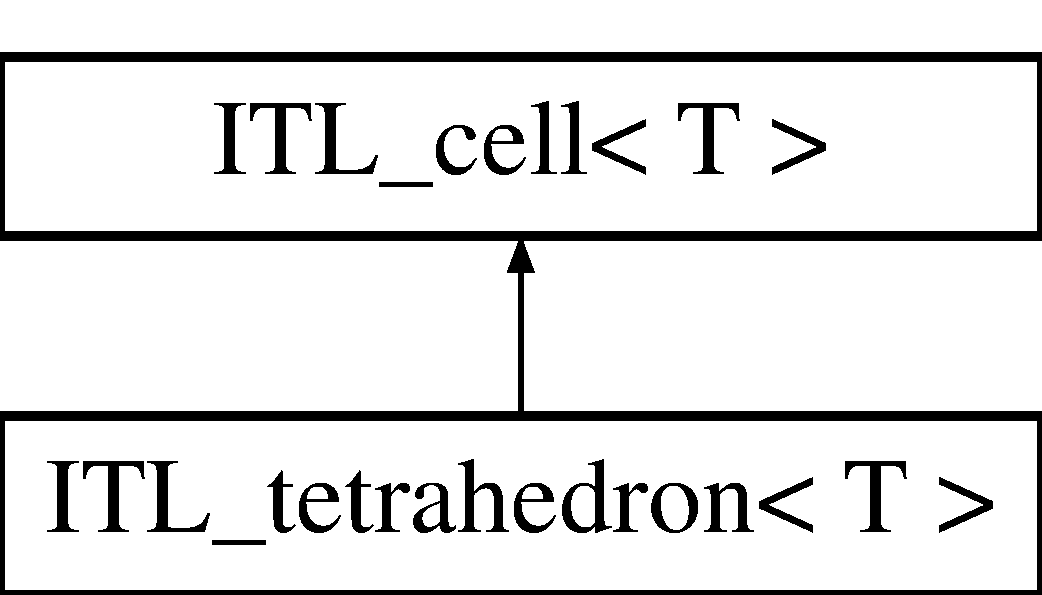
\includegraphics[height=2cm]{classITL__tetrahedron}
\end{center}
\end{figure}


\subsection{Detailed Description}
\subsubsection*{template$<$class T$>$ class ITL\_\-tetrahedron$<$ T $>$}

Tetrahedron class inherited from \hyperlink{classITL__cell}{ITL\_\-cell}. Encapsulates a tetrahedral unit of an unstructured grid. Created on: Apr 28, 2011 \begin{DoxyAuthor}{Author}
Abon 

Teng-\/Yok 
\end{DoxyAuthor}


Definition at line 13 of file ITL\_\-tetrahedron.h.



The documentation for this class was generated from the following file:\begin{DoxyCompactItemize}
\item 
/home/abon/Code/workspace\_\-unix/ITL\_\-repo/include/\hyperlink{ITL__tetrahedron_8h}{ITL\_\-tetrahedron.h}\end{DoxyCompactItemize}

\hypertarget{classITL__util}{
\section{ITL\_\-util$<$ T $>$ Class Template Reference}
\label{classITL__util}\index{ITL\_\-util@{ITL\_\-util}}
}


Utility class for the ITL library.  




{\ttfamily \#include $<$ITL\_\-util.h$>$}

\subsection*{Static Public Member Functions}
\begin{DoxyCompactItemize}
\item 
static T \hyperlink{classITL__util_a7d3b943bbe22704d2ac9d62fd8820b90}{clamp} (T val, T \hyperlink{MainIT__regvector_8cpp_abb1e2dad97264e859f3ee8af1341d68c}{low}, T \hyperlink{MainIT__regvector_8cpp_a2012a18ba7a98e566c072356d03c4240}{high})
\item 
static T \hyperlink{classITL__util_af15f3ba814e5e45277141747f9e16133}{mirror} (T val, T \hyperlink{MainIT__regvector_8cpp_abb1e2dad97264e859f3ee8af1341d68c}{low}, T \hyperlink{MainIT__regvector_8cpp_a2012a18ba7a98e566c072356d03c4240}{high})
\item 
static T \hyperlink{classITL__util_a0ae10172a5e09f46ff2d280d1f1d41b0}{Min} (T $\ast$array, int len)
\item 
static T \hyperlink{classITL__util_a162025a233f6ec9ca5bf9218390e8ad3}{Max} (T $\ast$array, int len)
\item 
static T \hyperlink{classITL__util_aad5bdd0ab06d36d4119e05ec2786005b}{sum} (T $\ast$array, int len)
\item 
static T \hyperlink{classITL__util_a9d64af43f6c6d4ebbbb794c6a95c12d6}{prod} (T $\ast$array, int len)
\item 
static void \hyperlink{classITL__util_aa99e2c6682db5444c25bacf428d6d1b9}{fill} (T $\ast$array, int len, T val)
\item 
static T $\ast$ \hyperlink{classITL__util_a8d0970f66d8443b106ec3b2b56008193}{addArrays} (T $\ast$one, T $\ast$two, int len)
\item 
static T $\ast$ \hyperlink{classITL__util_af3fcfd1766bf96813b009adc8abb5a7b}{subtractArrays} (T $\ast$one, T $\ast$two, int len)
\item 
static void \hyperlink{classITL__util_ab67646a3fb9b2749d2f763125ccb1dfa}{addArrayScalar} (T $\ast$array, T scalar, int len)
\item 
static void \hyperlink{classITL__util_a447741f40abd631431a41ff21a3f77b8}{subtractArrayScalar} (T $\ast$array, T scalar, int len)
\item 
static double \hyperlink{classITL__util_a46636a5a7bb9b109b342e403825c8ea9}{startTimer} ()
\begin{DoxyCompactList}\small\item\em Start Time computation. \item\end{DoxyCompactList}\item 
static double \hyperlink{classITL__util_aedbe31ffc820a9a99f4fbcea35f184ca}{endTimer} (clock\_\-t startTime)
\begin{DoxyCompactList}\small\item\em Complete Time computation. \item\end{DoxyCompactList}\end{DoxyCompactItemize}


\subsection{Detailed Description}
\subsubsection*{template$<$class T$>$ class ITL\_\-util$<$ T $>$}

Utility class for the ITL library. A basic utility class which implements basic array operations, timing calculation etc. Created on: Nov 22, 2010. \begin{DoxyAuthor}{Author}
Abon 

Teng-\/Yok 
\end{DoxyAuthor}


Definition at line 17 of file ITL\_\-util.h.



\subsection{Member Function Documentation}
\hypertarget{classITL__util_a8d0970f66d8443b106ec3b2b56008193}{
\index{ITL\_\-util@{ITL\_\-util}!addArrays@{addArrays}}
\index{addArrays@{addArrays}!ITL_util@{ITL\_\-util}}
\subsubsection[{addArrays}]{\setlength{\rightskip}{0pt plus 5cm}template$<$class T $>$ static T$\ast$ {\bf ITL\_\-util}$<$ T $>$::addArrays (T $\ast$ {\em one}, \/  T $\ast$ {\em two}, \/  int {\em len})\hspace{0.3cm}{\ttfamily  \mbox{[}inline, static\mbox{]}}}}
\label{classITL__util_a8d0970f66d8443b106ec3b2b56008193}


Definition at line 87 of file ITL\_\-util.h.

\hypertarget{classITL__util_ab67646a3fb9b2749d2f763125ccb1dfa}{
\index{ITL\_\-util@{ITL\_\-util}!addArrayScalar@{addArrayScalar}}
\index{addArrayScalar@{addArrayScalar}!ITL_util@{ITL\_\-util}}
\subsubsection[{addArrayScalar}]{\setlength{\rightskip}{0pt plus 5cm}template$<$class T $>$ static void {\bf ITL\_\-util}$<$ T $>$::addArrayScalar (T $\ast$ {\em array}, \/  T {\em scalar}, \/  int {\em len})\hspace{0.3cm}{\ttfamily  \mbox{[}inline, static\mbox{]}}}}
\label{classITL__util_ab67646a3fb9b2749d2f763125ccb1dfa}


Definition at line 107 of file ITL\_\-util.h.

\hypertarget{classITL__util_a7d3b943bbe22704d2ac9d62fd8820b90}{
\index{ITL\_\-util@{ITL\_\-util}!clamp@{clamp}}
\index{clamp@{clamp}!ITL_util@{ITL\_\-util}}
\subsubsection[{clamp}]{\setlength{\rightskip}{0pt plus 5cm}template$<$class T $>$ static T {\bf ITL\_\-util}$<$ T $>$::clamp (T {\em val}, \/  T {\em low}, \/  T {\em high})\hspace{0.3cm}{\ttfamily  \mbox{[}inline, static\mbox{]}}}}
\label{classITL__util_a7d3b943bbe22704d2ac9d62fd8820b90}


Definition at line 24 of file ITL\_\-util.h.

\hypertarget{classITL__util_aedbe31ffc820a9a99f4fbcea35f184ca}{
\index{ITL\_\-util@{ITL\_\-util}!endTimer@{endTimer}}
\index{endTimer@{endTimer}!ITL_util@{ITL\_\-util}}
\subsubsection[{endTimer}]{\setlength{\rightskip}{0pt plus 5cm}template$<$class T $>$ static double {\bf ITL\_\-util}$<$ T $>$::endTimer (clock\_\-t {\em startTime})\hspace{0.3cm}{\ttfamily  \mbox{[}inline, static\mbox{]}}}}
\label{classITL__util_aedbe31ffc820a9a99f4fbcea35f184ca}


Complete Time computation. 


\begin{DoxyParams}{Parameters}
\item[{\em startTime}]Recored time at start point \end{DoxyParams}
\begin{DoxyReturn}{Returns}
computed time in seconds from start to end. 
\end{DoxyReturn}


Definition at line 136 of file ITL\_\-util.h.

\hypertarget{classITL__util_aa99e2c6682db5444c25bacf428d6d1b9}{
\index{ITL\_\-util@{ITL\_\-util}!fill@{fill}}
\index{fill@{fill}!ITL_util@{ITL\_\-util}}
\subsubsection[{fill}]{\setlength{\rightskip}{0pt plus 5cm}template$<$class T $>$ static void {\bf ITL\_\-util}$<$ T $>$::fill (T $\ast$ {\em array}, \/  int {\em len}, \/  T {\em val})\hspace{0.3cm}{\ttfamily  \mbox{[}inline, static\mbox{]}}}}
\label{classITL__util_aa99e2c6682db5444c25bacf428d6d1b9}


Definition at line 79 of file ITL\_\-util.h.

\hypertarget{classITL__util_a162025a233f6ec9ca5bf9218390e8ad3}{
\index{ITL\_\-util@{ITL\_\-util}!Max@{Max}}
\index{Max@{Max}!ITL_util@{ITL\_\-util}}
\subsubsection[{Max}]{\setlength{\rightskip}{0pt plus 5cm}template$<$class T $>$ static T {\bf ITL\_\-util}$<$ T $>$::Max (T $\ast$ {\em array}, \/  int {\em len})\hspace{0.3cm}{\ttfamily  \mbox{[}inline, static\mbox{]}}}}
\label{classITL__util_a162025a233f6ec9ca5bf9218390e8ad3}


Definition at line 49 of file ITL\_\-util.h.

\hypertarget{classITL__util_a0ae10172a5e09f46ff2d280d1f1d41b0}{
\index{ITL\_\-util@{ITL\_\-util}!Min@{Min}}
\index{Min@{Min}!ITL_util@{ITL\_\-util}}
\subsubsection[{Min}]{\setlength{\rightskip}{0pt plus 5cm}template$<$class T $>$ static T {\bf ITL\_\-util}$<$ T $>$::Min (T $\ast$ {\em array}, \/  int {\em len})\hspace{0.3cm}{\ttfamily  \mbox{[}inline, static\mbox{]}}}}
\label{classITL__util_a0ae10172a5e09f46ff2d280d1f1d41b0}


Definition at line 38 of file ITL\_\-util.h.

\hypertarget{classITL__util_af15f3ba814e5e45277141747f9e16133}{
\index{ITL\_\-util@{ITL\_\-util}!mirror@{mirror}}
\index{mirror@{mirror}!ITL_util@{ITL\_\-util}}
\subsubsection[{mirror}]{\setlength{\rightskip}{0pt plus 5cm}template$<$class T $>$ static T {\bf ITL\_\-util}$<$ T $>$::mirror (T {\em val}, \/  T {\em low}, \/  T {\em high})\hspace{0.3cm}{\ttfamily  \mbox{[}inline, static\mbox{]}}}}
\label{classITL__util_af15f3ba814e5e45277141747f9e16133}


Definition at line 31 of file ITL\_\-util.h.

\hypertarget{classITL__util_a9d64af43f6c6d4ebbbb794c6a95c12d6}{
\index{ITL\_\-util@{ITL\_\-util}!prod@{prod}}
\index{prod@{prod}!ITL_util@{ITL\_\-util}}
\subsubsection[{prod}]{\setlength{\rightskip}{0pt plus 5cm}template$<$class T $>$ static T {\bf ITL\_\-util}$<$ T $>$::prod (T $\ast$ {\em array}, \/  int {\em len})\hspace{0.3cm}{\ttfamily  \mbox{[}inline, static\mbox{]}}}}
\label{classITL__util_a9d64af43f6c6d4ebbbb794c6a95c12d6}


Definition at line 70 of file ITL\_\-util.h.

\hypertarget{classITL__util_a46636a5a7bb9b109b342e403825c8ea9}{
\index{ITL\_\-util@{ITL\_\-util}!startTimer@{startTimer}}
\index{startTimer@{startTimer}!ITL_util@{ITL\_\-util}}
\subsubsection[{startTimer}]{\setlength{\rightskip}{0pt plus 5cm}template$<$class T $>$ static double {\bf ITL\_\-util}$<$ T $>$::startTimer ()\hspace{0.3cm}{\ttfamily  \mbox{[}inline, static\mbox{]}}}}
\label{classITL__util_a46636a5a7bb9b109b342e403825c8ea9}


Start Time computation. 



Definition at line 126 of file ITL\_\-util.h.

\hypertarget{classITL__util_af3fcfd1766bf96813b009adc8abb5a7b}{
\index{ITL\_\-util@{ITL\_\-util}!subtractArrays@{subtractArrays}}
\index{subtractArrays@{subtractArrays}!ITL_util@{ITL\_\-util}}
\subsubsection[{subtractArrays}]{\setlength{\rightskip}{0pt plus 5cm}template$<$class T $>$ static T$\ast$ {\bf ITL\_\-util}$<$ T $>$::subtractArrays (T $\ast$ {\em one}, \/  T $\ast$ {\em two}, \/  int {\em len})\hspace{0.3cm}{\ttfamily  \mbox{[}inline, static\mbox{]}}}}
\label{classITL__util_af3fcfd1766bf96813b009adc8abb5a7b}


Definition at line 97 of file ITL\_\-util.h.

\hypertarget{classITL__util_a447741f40abd631431a41ff21a3f77b8}{
\index{ITL\_\-util@{ITL\_\-util}!subtractArrayScalar@{subtractArrayScalar}}
\index{subtractArrayScalar@{subtractArrayScalar}!ITL_util@{ITL\_\-util}}
\subsubsection[{subtractArrayScalar}]{\setlength{\rightskip}{0pt plus 5cm}template$<$class T $>$ static void {\bf ITL\_\-util}$<$ T $>$::subtractArrayScalar (T $\ast$ {\em array}, \/  T {\em scalar}, \/  int {\em len})\hspace{0.3cm}{\ttfamily  \mbox{[}inline, static\mbox{]}}}}
\label{classITL__util_a447741f40abd631431a41ff21a3f77b8}


Definition at line 115 of file ITL\_\-util.h.

\hypertarget{classITL__util_aad5bdd0ab06d36d4119e05ec2786005b}{
\index{ITL\_\-util@{ITL\_\-util}!sum@{sum}}
\index{sum@{sum}!ITL_util@{ITL\_\-util}}
\subsubsection[{sum}]{\setlength{\rightskip}{0pt plus 5cm}template$<$class T $>$ static T {\bf ITL\_\-util}$<$ T $>$::sum (T $\ast$ {\em array}, \/  int {\em len})\hspace{0.3cm}{\ttfamily  \mbox{[}inline, static\mbox{]}}}}
\label{classITL__util_aad5bdd0ab06d36d4119e05ec2786005b}


Definition at line 61 of file ITL\_\-util.h.



The documentation for this class was generated from the following file:\begin{DoxyCompactItemize}
\item 
/home/abon/Code/workspace\_\-unix/ITL\_\-repo/include/\hyperlink{ITL__util_8h}{ITL\_\-util.h}\end{DoxyCompactItemize}

\hypertarget{structline__2d}{
\section{line\_\-2d Struct Reference}
\label{structline__2d}\index{line\_\-2d@{line\_\-2d}}
}


{\ttfamily \#include $<$ITL\_\-vectormatrix.h$>$}

\subsection*{Public Attributes}
\begin{DoxyCompactItemize}
\item 
\hyperlink{classVECTOR2}{VECTOR2} \hyperlink{structline__2d_a9bdc6824a8ea1f195b4286d4155dfa5d}{start}
\item 
\hyperlink{classVECTOR2}{VECTOR2} \hyperlink{structline__2d_a6147946f41a7b50692c7bfe9a1f51360}{end}
\end{DoxyCompactItemize}


\subsection{Detailed Description}


Definition at line 53 of file ITL\_\-vectormatrix.h.



\subsection{Member Data Documentation}
\hypertarget{structline__2d_a6147946f41a7b50692c7bfe9a1f51360}{
\index{line\_\-2d@{line\_\-2d}!end@{end}}
\index{end@{end}!line_2d@{line\_\-2d}}
\subsubsection[{end}]{\setlength{\rightskip}{0pt plus 5cm}{\bf VECTOR2} {\bf line\_\-2d::end}}}
\label{structline__2d_a6147946f41a7b50692c7bfe9a1f51360}


Definition at line 55 of file ITL\_\-vectormatrix.h.

\hypertarget{structline__2d_a9bdc6824a8ea1f195b4286d4155dfa5d}{
\index{line\_\-2d@{line\_\-2d}!start@{start}}
\index{start@{start}!line_2d@{line\_\-2d}}
\subsubsection[{start}]{\setlength{\rightskip}{0pt plus 5cm}{\bf VECTOR2} {\bf line\_\-2d::start}}}
\label{structline__2d_a9bdc6824a8ea1f195b4286d4155dfa5d}


Definition at line 54 of file ITL\_\-vectormatrix.h.



The documentation for this struct was generated from the following file:\begin{DoxyCompactItemize}
\item 
/home/abon/Code/workspace\_\-unix/ITL\_\-repo/include/\hyperlink{ITL__vectormatrix_8h}{ITL\_\-vectormatrix.h}\end{DoxyCompactItemize}

\hypertarget{classMATRIX3}{
\section{MATRIX3 Class Reference}
\label{classMATRIX3}\index{MATRIX3@{MATRIX3}}
}


{\ttfamily \#include $<$ITL\_\-vectormatrix.h$>$}

\subsection*{Public Member Functions}
\begin{DoxyCompactItemize}
\item 
\hyperlink{classMATRIX3_a6c4e88b8dc71944f2819d809c8af33db}{MATRIX3} ()
\item 
\hyperlink{classMATRIX3_ae537368e20b379c611c2897396ca879b}{MATRIX3} (const \hyperlink{classVECTOR3}{VECTOR3} \&v0, const \hyperlink{classVECTOR3}{VECTOR3} \&v1, const \hyperlink{classVECTOR3}{VECTOR3} \&v2)
\item 
int \hyperlink{classMATRIX3_ad39ac7b76a15a678c8a74dc8a95e0754}{Dimension} () const 
\item 
\hyperlink{classVECTOR3}{VECTOR3} \& \hyperlink{classMATRIX3_a568cfeb7a853e8f1c6437046ab6c5cb1}{operator\mbox{[}$\,$\mbox{]}} (const int i)
\item 
\hyperlink{classVECTOR3}{VECTOR3} \hyperlink{classMATRIX3_ae4ad5d725102c93251dd1da56dd9fab8}{operator()} (const int i) const 
\item 
float \hyperlink{classMATRIX3_a4c879e29653a167d5af33e297b46bdd4}{operator()} (const int i, const int j) const 
\item 
\hyperlink{classMATRIX3}{MATRIX3} \& \hyperlink{classMATRIX3_a6154de213d293b953f2be789a86a58eb}{operator=} (const \hyperlink{classMATRIX3}{MATRIX3} \&m0)
\item 
void \hyperlink{classMATRIX3_af765df1cefaaacc2e8f1e27f2041ca15}{Identity} ()
\end{DoxyCompactItemize}
\subsection*{Private Attributes}
\begin{DoxyCompactItemize}
\item 
\hyperlink{classVECTOR3}{VECTOR3} \hyperlink{classMATRIX3_ad05b011bf87af20da045df5640013017}{mat} \mbox{[}3\mbox{]}
\end{DoxyCompactItemize}


\subsection{Detailed Description}


Definition at line 132 of file ITL\_\-vectormatrix.h.



\subsection{Constructor \& Destructor Documentation}
\hypertarget{classMATRIX3_a6c4e88b8dc71944f2819d809c8af33db}{
\index{MATRIX3@{MATRIX3}!MATRIX3@{MATRIX3}}
\index{MATRIX3@{MATRIX3}!MATRIX3@{MATRIX3}}
\subsubsection[{MATRIX3}]{\setlength{\rightskip}{0pt plus 5cm}MATRIX3::MATRIX3 ()\hspace{0.3cm}{\ttfamily  \mbox{[}inline\mbox{]}}}}
\label{classMATRIX3_a6c4e88b8dc71944f2819d809c8af33db}


Definition at line 139 of file ITL\_\-vectormatrix.h.

\hypertarget{classMATRIX3_ae537368e20b379c611c2897396ca879b}{
\index{MATRIX3@{MATRIX3}!MATRIX3@{MATRIX3}}
\index{MATRIX3@{MATRIX3}!MATRIX3@{MATRIX3}}
\subsubsection[{MATRIX3}]{\setlength{\rightskip}{0pt plus 5cm}MATRIX3::MATRIX3 (const {\bf VECTOR3} \& {\em v0}, \/  const {\bf VECTOR3} \& {\em v1}, \/  const {\bf VECTOR3} \& {\em v2})\hspace{0.3cm}{\ttfamily  \mbox{[}inline\mbox{]}}}}
\label{classMATRIX3_ae537368e20b379c611c2897396ca879b}


Definition at line 141 of file ITL\_\-vectormatrix.h.



\subsection{Member Function Documentation}
\hypertarget{classMATRIX3_ad39ac7b76a15a678c8a74dc8a95e0754}{
\index{MATRIX3@{MATRIX3}!Dimension@{Dimension}}
\index{Dimension@{Dimension}!MATRIX3@{MATRIX3}}
\subsubsection[{Dimension}]{\setlength{\rightskip}{0pt plus 5cm}int MATRIX3::Dimension () const\hspace{0.3cm}{\ttfamily  \mbox{[}inline\mbox{]}}}}
\label{classMATRIX3_ad39ac7b76a15a678c8a74dc8a95e0754}


Definition at line 143 of file ITL\_\-vectormatrix.h.

\hypertarget{classMATRIX3_af765df1cefaaacc2e8f1e27f2041ca15}{
\index{MATRIX3@{MATRIX3}!Identity@{Identity}}
\index{Identity@{Identity}!MATRIX3@{MATRIX3}}
\subsubsection[{Identity}]{\setlength{\rightskip}{0pt plus 5cm}void MATRIX3::Identity ()}}
\label{classMATRIX3_af765df1cefaaacc2e8f1e27f2041ca15}


Definition at line 79 of file ITL\_\-vectormatrix.cpp.

\hypertarget{classMATRIX3_a4c879e29653a167d5af33e297b46bdd4}{
\index{MATRIX3@{MATRIX3}!operator()@{operator()}}
\index{operator()@{operator()}!MATRIX3@{MATRIX3}}
\subsubsection[{operator()}]{\setlength{\rightskip}{0pt plus 5cm}float MATRIX3::operator() (const int {\em i}, \/  const int {\em j}) const\hspace{0.3cm}{\ttfamily  \mbox{[}inline\mbox{]}}}}
\label{classMATRIX3_a4c879e29653a167d5af33e297b46bdd4}


Definition at line 150 of file ITL\_\-vectormatrix.h.

\hypertarget{classMATRIX3_ae4ad5d725102c93251dd1da56dd9fab8}{
\index{MATRIX3@{MATRIX3}!operator()@{operator()}}
\index{operator()@{operator()}!MATRIX3@{MATRIX3}}
\subsubsection[{operator()}]{\setlength{\rightskip}{0pt plus 5cm}{\bf VECTOR3} MATRIX3::operator() (const int {\em i}) const\hspace{0.3cm}{\ttfamily  \mbox{[}inline\mbox{]}}}}
\label{classMATRIX3_ae4ad5d725102c93251dd1da56dd9fab8}


Definition at line 148 of file ITL\_\-vectormatrix.h.

\hypertarget{classMATRIX3_a6154de213d293b953f2be789a86a58eb}{
\index{MATRIX3@{MATRIX3}!operator=@{operator=}}
\index{operator=@{operator=}!MATRIX3@{MATRIX3}}
\subsubsection[{operator=}]{\setlength{\rightskip}{0pt plus 5cm}{\bf MATRIX3}\& MATRIX3::operator= (const {\bf MATRIX3} \& {\em m0})\hspace{0.3cm}{\ttfamily  \mbox{[}inline\mbox{]}}}}
\label{classMATRIX3_a6154de213d293b953f2be789a86a58eb}


Definition at line 152 of file ITL\_\-vectormatrix.h.

\hypertarget{classMATRIX3_a568cfeb7a853e8f1c6437046ab6c5cb1}{
\index{MATRIX3@{MATRIX3}!operator\mbox{[}\mbox{]}@{operator[]}}
\index{operator\mbox{[}\mbox{]}@{operator[]}!MATRIX3@{MATRIX3}}
\subsubsection[{operator[]}]{\setlength{\rightskip}{0pt plus 5cm}{\bf VECTOR3}\& MATRIX3::operator\mbox{[}$\,$\mbox{]} (const int {\em i})\hspace{0.3cm}{\ttfamily  \mbox{[}inline\mbox{]}}}}
\label{classMATRIX3_a568cfeb7a853e8f1c6437046ab6c5cb1}


Definition at line 145 of file ITL\_\-vectormatrix.h.



\subsection{Member Data Documentation}
\hypertarget{classMATRIX3_ad05b011bf87af20da045df5640013017}{
\index{MATRIX3@{MATRIX3}!mat@{mat}}
\index{mat@{mat}!MATRIX3@{MATRIX3}}
\subsubsection[{mat}]{\setlength{\rightskip}{0pt plus 5cm}{\bf VECTOR3} {\bf MATRIX3::mat}\mbox{[}3\mbox{]}\hspace{0.3cm}{\ttfamily  \mbox{[}private\mbox{]}}}}
\label{classMATRIX3_ad05b011bf87af20da045df5640013017}


Definition at line 135 of file ITL\_\-vectormatrix.h.



The documentation for this class was generated from the following files:\begin{DoxyCompactItemize}
\item 
/home/abon/Code/workspace\_\-unix/ITL\_\-repo/include/\hyperlink{ITL__vectormatrix_8h}{ITL\_\-vectormatrix.h}\item 
/home/abon/Code/workspace\_\-unix/ITL\_\-repo/src/\hyperlink{ITL__vectormatrix_8cpp}{ITL\_\-vectormatrix.cpp}\end{DoxyCompactItemize}

\hypertarget{classMATRIX4}{
\section{MATRIX4 Class Reference}
\label{classMATRIX4}\index{MATRIX4@{MATRIX4}}
}


{\ttfamily \#include $<$ITL\_\-vectormatrix.h$>$}

\subsection*{Public Member Functions}
\begin{DoxyCompactItemize}
\item 
\hyperlink{classMATRIX4_adbac71e9c60831aec2a35c43e1af6ca1}{MATRIX4} ()
\item 
\hyperlink{classMATRIX4_a5d47eec9650ec2cbb6ba3f347e63b3a9}{MATRIX4} (const \hyperlink{classVECTOR4}{VECTOR4} \&v0, const \hyperlink{classVECTOR4}{VECTOR4} \&v1, const \hyperlink{classVECTOR4}{VECTOR4} \&v2, const \hyperlink{classVECTOR4}{VECTOR4} \&v3)
\item 
int \hyperlink{classMATRIX4_af2d9ab8c4cfa8ccd705af3e0f2dd122d}{Dimension} () const 
\item 
\hyperlink{classVECTOR4}{VECTOR4} \& \hyperlink{classMATRIX4_ab266bb9fde86ff7085abb57bd7acbc25}{operator\mbox{[}$\,$\mbox{]}} (int i)
\item 
\hyperlink{classVECTOR4}{VECTOR4} \hyperlink{classMATRIX4_aab1a056c9199cf7c956ffa17a1607033}{operator()} (const int i) const 
\item 
float \hyperlink{classMATRIX4_af31bcf17f6a09d2c14ca7e84f73728f3}{operator()} (const int i, const int j) const 
\item 
\hyperlink{classMATRIX4}{MATRIX4} \& \hyperlink{classMATRIX4_a74b1f4b9862b324d0bf3841ac4dbbfbe}{operator=} (const \hyperlink{classMATRIX4}{MATRIX4} \&m0)
\item 
\hyperlink{classMATRIX4}{MATRIX4} \& \hyperlink{classMATRIX4_a0eab7ae1f433432b3e931c08c74d6410}{operator=} (const \hyperlink{classMATRIX3}{MATRIX3} \&m0)
\item 
void \hyperlink{classMATRIX4_a1140fdbe58cd646997db65e742d21739}{Identity} ()
\end{DoxyCompactItemize}
\subsection*{Private Attributes}
\begin{DoxyCompactItemize}
\item 
\hyperlink{classVECTOR4}{VECTOR4} \hyperlink{classMATRIX4_ac593e924265eb8846b77402f46ee82dd}{mat} \mbox{[}4\mbox{]}
\end{DoxyCompactItemize}


\subsection{Detailed Description}


Definition at line 161 of file ITL\_\-vectormatrix.h.



\subsection{Constructor \& Destructor Documentation}
\hypertarget{classMATRIX4_adbac71e9c60831aec2a35c43e1af6ca1}{
\index{MATRIX4@{MATRIX4}!MATRIX4@{MATRIX4}}
\index{MATRIX4@{MATRIX4}!MATRIX4@{MATRIX4}}
\subsubsection[{MATRIX4}]{\setlength{\rightskip}{0pt plus 5cm}MATRIX4::MATRIX4 ()\hspace{0.3cm}{\ttfamily  \mbox{[}inline\mbox{]}}}}
\label{classMATRIX4_adbac71e9c60831aec2a35c43e1af6ca1}


Definition at line 169 of file ITL\_\-vectormatrix.h.

\hypertarget{classMATRIX4_a5d47eec9650ec2cbb6ba3f347e63b3a9}{
\index{MATRIX4@{MATRIX4}!MATRIX4@{MATRIX4}}
\index{MATRIX4@{MATRIX4}!MATRIX4@{MATRIX4}}
\subsubsection[{MATRIX4}]{\setlength{\rightskip}{0pt plus 5cm}MATRIX4::MATRIX4 (const {\bf VECTOR4} \& {\em v0}, \/  const {\bf VECTOR4} \& {\em v1}, \/  const {\bf VECTOR4} \& {\em v2}, \/  const {\bf VECTOR4} \& {\em v3})\hspace{0.3cm}{\ttfamily  \mbox{[}inline\mbox{]}}}}
\label{classMATRIX4_a5d47eec9650ec2cbb6ba3f347e63b3a9}


Definition at line 171 of file ITL\_\-vectormatrix.h.



\subsection{Member Function Documentation}
\hypertarget{classMATRIX4_af2d9ab8c4cfa8ccd705af3e0f2dd122d}{
\index{MATRIX4@{MATRIX4}!Dimension@{Dimension}}
\index{Dimension@{Dimension}!MATRIX4@{MATRIX4}}
\subsubsection[{Dimension}]{\setlength{\rightskip}{0pt plus 5cm}int MATRIX4::Dimension () const\hspace{0.3cm}{\ttfamily  \mbox{[}inline\mbox{]}}}}
\label{classMATRIX4_af2d9ab8c4cfa8ccd705af3e0f2dd122d}


Definition at line 174 of file ITL\_\-vectormatrix.h.

\hypertarget{classMATRIX4_a1140fdbe58cd646997db65e742d21739}{
\index{MATRIX4@{MATRIX4}!Identity@{Identity}}
\index{Identity@{Identity}!MATRIX4@{MATRIX4}}
\subsubsection[{Identity}]{\setlength{\rightskip}{0pt plus 5cm}void MATRIX4::Identity ()}}
\label{classMATRIX4_a1140fdbe58cd646997db65e742d21739}


Definition at line 92 of file ITL\_\-vectormatrix.cpp.

\hypertarget{classMATRIX4_af31bcf17f6a09d2c14ca7e84f73728f3}{
\index{MATRIX4@{MATRIX4}!operator()@{operator()}}
\index{operator()@{operator()}!MATRIX4@{MATRIX4}}
\subsubsection[{operator()}]{\setlength{\rightskip}{0pt plus 5cm}float MATRIX4::operator() (const int {\em i}, \/  const int {\em j}) const\hspace{0.3cm}{\ttfamily  \mbox{[}inline\mbox{]}}}}
\label{classMATRIX4_af31bcf17f6a09d2c14ca7e84f73728f3}


Definition at line 181 of file ITL\_\-vectormatrix.h.

\hypertarget{classMATRIX4_aab1a056c9199cf7c956ffa17a1607033}{
\index{MATRIX4@{MATRIX4}!operator()@{operator()}}
\index{operator()@{operator()}!MATRIX4@{MATRIX4}}
\subsubsection[{operator()}]{\setlength{\rightskip}{0pt plus 5cm}{\bf VECTOR4} MATRIX4::operator() (const int {\em i}) const\hspace{0.3cm}{\ttfamily  \mbox{[}inline\mbox{]}}}}
\label{classMATRIX4_aab1a056c9199cf7c956ffa17a1607033}


Definition at line 179 of file ITL\_\-vectormatrix.h.

\hypertarget{classMATRIX4_a0eab7ae1f433432b3e931c08c74d6410}{
\index{MATRIX4@{MATRIX4}!operator=@{operator=}}
\index{operator=@{operator=}!MATRIX4@{MATRIX4}}
\subsubsection[{operator=}]{\setlength{\rightskip}{0pt plus 5cm}{\bf MATRIX4}\& MATRIX4::operator= (const {\bf MATRIX3} \& {\em m0})\hspace{0.3cm}{\ttfamily  \mbox{[}inline\mbox{]}}}}
\label{classMATRIX4_a0eab7ae1f433432b3e931c08c74d6410}


Definition at line 186 of file ITL\_\-vectormatrix.h.

\hypertarget{classMATRIX4_a74b1f4b9862b324d0bf3841ac4dbbfbe}{
\index{MATRIX4@{MATRIX4}!operator=@{operator=}}
\index{operator=@{operator=}!MATRIX4@{MATRIX4}}
\subsubsection[{operator=}]{\setlength{\rightskip}{0pt plus 5cm}{\bf MATRIX4}\& MATRIX4::operator= (const {\bf MATRIX4} \& {\em m0})\hspace{0.3cm}{\ttfamily  \mbox{[}inline\mbox{]}}}}
\label{classMATRIX4_a74b1f4b9862b324d0bf3841ac4dbbfbe}


Definition at line 183 of file ITL\_\-vectormatrix.h.

\hypertarget{classMATRIX4_ab266bb9fde86ff7085abb57bd7acbc25}{
\index{MATRIX4@{MATRIX4}!operator\mbox{[}\mbox{]}@{operator[]}}
\index{operator\mbox{[}\mbox{]}@{operator[]}!MATRIX4@{MATRIX4}}
\subsubsection[{operator[]}]{\setlength{\rightskip}{0pt plus 5cm}{\bf VECTOR4}\& MATRIX4::operator\mbox{[}$\,$\mbox{]} (int {\em i})\hspace{0.3cm}{\ttfamily  \mbox{[}inline\mbox{]}}}}
\label{classMATRIX4_ab266bb9fde86ff7085abb57bd7acbc25}


Definition at line 176 of file ITL\_\-vectormatrix.h.



\subsection{Member Data Documentation}
\hypertarget{classMATRIX4_ac593e924265eb8846b77402f46ee82dd}{
\index{MATRIX4@{MATRIX4}!mat@{mat}}
\index{mat@{mat}!MATRIX4@{MATRIX4}}
\subsubsection[{mat}]{\setlength{\rightskip}{0pt plus 5cm}{\bf VECTOR4} {\bf MATRIX4::mat}\mbox{[}4\mbox{]}\hspace{0.3cm}{\ttfamily  \mbox{[}private\mbox{]}}}}
\label{classMATRIX4_ac593e924265eb8846b77402f46ee82dd}


Definition at line 165 of file ITL\_\-vectormatrix.h.



The documentation for this class was generated from the following files:\begin{DoxyCompactItemize}
\item 
/home/abon/Code/workspace\_\-unix/ITL\_\-repo/include/\hyperlink{ITL__vectormatrix_8h}{ITL\_\-vectormatrix.h}\item 
/home/abon/Code/workspace\_\-unix/ITL\_\-repo/src/\hyperlink{ITL__vectormatrix_8cpp}{ITL\_\-vectormatrix.cpp}\end{DoxyCompactItemize}

\hypertarget{classVECTOR2}{
\section{VECTOR2 Class Reference}
\label{classVECTOR2}\index{VECTOR2@{VECTOR2}}
}


{\ttfamily \#include $<$ITL\_\-vectormatrix.h$>$}

\subsection*{Public Member Functions}
\begin{DoxyCompactItemize}
\item 
\hyperlink{classVECTOR2_a321837bdc28f77b6958cb2bccb41fc92}{VECTOR2} ()
\item 
\hyperlink{classVECTOR2_a7ad80af0b479f2c9fc1cbe8c3c912e13}{VECTOR2} (const float x0, const float x1)
\item 
int \hyperlink{classVECTOR2_a6c5930e1fbcbbb6b9fea0db80b83a515}{Dimension} () const 
\item 
float \& \hyperlink{classVECTOR2_af6d23b6a2fd595314c7b0fbf83ad723a}{operator\mbox{[}$\,$\mbox{]}} (const int i)
\item 
float \hyperlink{classVECTOR2_ab99d8f6de7559cc0ce413820449dff33}{operator()} (const int i) const 
\item 
const \hyperlink{classVECTOR2}{VECTOR2} \& \hyperlink{classVECTOR2_a89f1c28aa5e14ab1f32d12d9d68b4648}{operator=} (const \hyperlink{classVECTOR2}{VECTOR2} \&v0)
\item 
void \hyperlink{classVECTOR2_aa1c6e9606376454625184342925a6fce}{Zero} ()
\item 
void \hyperlink{classVECTOR2_acb0b60a765f7c11fbc43d6559f8eae19}{Set} (const float x0, const float x1)
\end{DoxyCompactItemize}
\subsection*{Private Attributes}
\begin{DoxyCompactItemize}
\item 
float \hyperlink{classVECTOR2_a2a652a951bed082365807c39e702d79a}{vec} \mbox{[}2\mbox{]}
\end{DoxyCompactItemize}


\subsection{Detailed Description}


Definition at line 27 of file ITL\_\-vectormatrix.h.



\subsection{Constructor \& Destructor Documentation}
\hypertarget{classVECTOR2_a321837bdc28f77b6958cb2bccb41fc92}{
\index{VECTOR2@{VECTOR2}!VECTOR2@{VECTOR2}}
\index{VECTOR2@{VECTOR2}!VECTOR2@{VECTOR2}}
\subsubsection[{VECTOR2}]{\setlength{\rightskip}{0pt plus 5cm}VECTOR2::VECTOR2 ()\hspace{0.3cm}{\ttfamily  \mbox{[}inline\mbox{]}}}}
\label{classVECTOR2_a321837bdc28f77b6958cb2bccb41fc92}


Definition at line 33 of file ITL\_\-vectormatrix.h.

\hypertarget{classVECTOR2_a7ad80af0b479f2c9fc1cbe8c3c912e13}{
\index{VECTOR2@{VECTOR2}!VECTOR2@{VECTOR2}}
\index{VECTOR2@{VECTOR2}!VECTOR2@{VECTOR2}}
\subsubsection[{VECTOR2}]{\setlength{\rightskip}{0pt plus 5cm}VECTOR2::VECTOR2 (const float {\em x0}, \/  const float {\em x1})\hspace{0.3cm}{\ttfamily  \mbox{[}inline\mbox{]}}}}
\label{classVECTOR2_a7ad80af0b479f2c9fc1cbe8c3c912e13}


Definition at line 35 of file ITL\_\-vectormatrix.h.



\subsection{Member Function Documentation}
\hypertarget{classVECTOR2_a6c5930e1fbcbbb6b9fea0db80b83a515}{
\index{VECTOR2@{VECTOR2}!Dimension@{Dimension}}
\index{Dimension@{Dimension}!VECTOR2@{VECTOR2}}
\subsubsection[{Dimension}]{\setlength{\rightskip}{0pt plus 5cm}int VECTOR2::Dimension () const\hspace{0.3cm}{\ttfamily  \mbox{[}inline\mbox{]}}}}
\label{classVECTOR2_a6c5930e1fbcbbb6b9fea0db80b83a515}


Definition at line 37 of file ITL\_\-vectormatrix.h.

\hypertarget{classVECTOR2_ab99d8f6de7559cc0ce413820449dff33}{
\index{VECTOR2@{VECTOR2}!operator()@{operator()}}
\index{operator()@{operator()}!VECTOR2@{VECTOR2}}
\subsubsection[{operator()}]{\setlength{\rightskip}{0pt plus 5cm}float VECTOR2::operator() (const int {\em i}) const\hspace{0.3cm}{\ttfamily  \mbox{[}inline\mbox{]}}}}
\label{classVECTOR2_ab99d8f6de7559cc0ce413820449dff33}


Definition at line 41 of file ITL\_\-vectormatrix.h.

\hypertarget{classVECTOR2_a89f1c28aa5e14ab1f32d12d9d68b4648}{
\index{VECTOR2@{VECTOR2}!operator=@{operator=}}
\index{operator=@{operator=}!VECTOR2@{VECTOR2}}
\subsubsection[{operator=}]{\setlength{\rightskip}{0pt plus 5cm}const {\bf VECTOR2}\& VECTOR2::operator= (const {\bf VECTOR2} \& {\em v0})\hspace{0.3cm}{\ttfamily  \mbox{[}inline\mbox{]}}}}
\label{classVECTOR2_a89f1c28aa5e14ab1f32d12d9d68b4648}


Definition at line 43 of file ITL\_\-vectormatrix.h.

\hypertarget{classVECTOR2_af6d23b6a2fd595314c7b0fbf83ad723a}{
\index{VECTOR2@{VECTOR2}!operator\mbox{[}\mbox{]}@{operator[]}}
\index{operator\mbox{[}\mbox{]}@{operator[]}!VECTOR2@{VECTOR2}}
\subsubsection[{operator[]}]{\setlength{\rightskip}{0pt plus 5cm}float\& VECTOR2::operator\mbox{[}$\,$\mbox{]} (const int {\em i})\hspace{0.3cm}{\ttfamily  \mbox{[}inline\mbox{]}}}}
\label{classVECTOR2_af6d23b6a2fd595314c7b0fbf83ad723a}


Definition at line 39 of file ITL\_\-vectormatrix.h.

\hypertarget{classVECTOR2_acb0b60a765f7c11fbc43d6559f8eae19}{
\index{VECTOR2@{VECTOR2}!Set@{Set}}
\index{Set@{Set}!VECTOR2@{VECTOR2}}
\subsubsection[{Set}]{\setlength{\rightskip}{0pt plus 5cm}void VECTOR2::Set (const float {\em x0}, \/  const float {\em x1})\hspace{0.3cm}{\ttfamily  \mbox{[}inline\mbox{]}}}}
\label{classVECTOR2_acb0b60a765f7c11fbc43d6559f8eae19}


Definition at line 48 of file ITL\_\-vectormatrix.h.

\hypertarget{classVECTOR2_aa1c6e9606376454625184342925a6fce}{
\index{VECTOR2@{VECTOR2}!Zero@{Zero}}
\index{Zero@{Zero}!VECTOR2@{VECTOR2}}
\subsubsection[{Zero}]{\setlength{\rightskip}{0pt plus 5cm}void VECTOR2::Zero ()\hspace{0.3cm}{\ttfamily  \mbox{[}inline\mbox{]}}}}
\label{classVECTOR2_aa1c6e9606376454625184342925a6fce}


Definition at line 46 of file ITL\_\-vectormatrix.h.



\subsection{Member Data Documentation}
\hypertarget{classVECTOR2_a2a652a951bed082365807c39e702d79a}{
\index{VECTOR2@{VECTOR2}!vec@{vec}}
\index{vec@{vec}!VECTOR2@{VECTOR2}}
\subsubsection[{vec}]{\setlength{\rightskip}{0pt plus 5cm}float {\bf VECTOR2::vec}\mbox{[}2\mbox{]}\hspace{0.3cm}{\ttfamily  \mbox{[}private\mbox{]}}}}
\label{classVECTOR2_a2a652a951bed082365807c39e702d79a}


Definition at line 30 of file ITL\_\-vectormatrix.h.



The documentation for this class was generated from the following file:\begin{DoxyCompactItemize}
\item 
/home/abon/Code/workspace\_\-unix/ITL\_\-repo/include/\hyperlink{ITL__vectormatrix_8h}{ITL\_\-vectormatrix.h}\end{DoxyCompactItemize}

\hypertarget{classVECTOR3}{
\section{VECTOR3 Class Reference}
\label{classVECTOR3}\index{VECTOR3@{VECTOR3}}
}


{\ttfamily \#include $<$ITL\_\-vectormatrix.h$>$}

\subsection*{Public Member Functions}
\begin{DoxyCompactItemize}
\item 
\hyperlink{classVECTOR3_a67df11517cf0d5f78bc4fbf7c8428c74}{VECTOR3} ()
\item 
\hyperlink{classVECTOR3_a36d21006a60aab59533ad9ef1f0dbec0}{VECTOR3} (const float x0, const float x1, const float x2)
\item 
void \hyperlink{classVECTOR3_a032256fc81e39310d30a38fb303ce48f}{Set} (const float x0, const float x1, const float x2)
\item 
int \hyperlink{classVECTOR3_a0f24d4dfcad2cf3bb11caa5a8f3bb758}{Dimension} () const 
\item 
float \hyperlink{classVECTOR3_ac05d9ef1b78723c720085c2d914bf504}{x} ()
\item 
float \hyperlink{classVECTOR3_aa6d52065fe15476ad2f169f93e8e4539}{y} ()
\item 
float \hyperlink{classVECTOR3_a8962966f79d06da320d958555cd7c98e}{z} ()
\item 
float \& \hyperlink{classVECTOR3_ad036f6898236422beeb85ea329ee510f}{operator\mbox{[}$\,$\mbox{]}} (const int i)
\item 
float \hyperlink{classVECTOR3_a3ed6b977aafcd21ffca8bbc081a55694}{operator()} (const int i) const 
\item 
bool \hyperlink{classVECTOR3_a4fd7d880a7bdab66567d23dccaaf27d4}{operator==} (const \hyperlink{classVECTOR3}{VECTOR3} \&v) const 
\item 
void \hyperlink{classVECTOR3_a55e86265b134a80232d1fb4f8857d3e2}{Zero} ()
\item 
float \hyperlink{classVECTOR3_ad0453425d5ddd7acc41e779e58292c82}{GetMag} ()
\item 
const \hyperlink{classVECTOR3}{VECTOR3} \& \hyperlink{classVECTOR3_a09838095d5261acb5d316ff1b1748c6a}{operator=} (const \hyperlink{classVECTOR3}{VECTOR3} \&v0)
\item 
float \hyperlink{classVECTOR3_ad3d4922b7faecfbf09a04e7ec63f8b97}{GetMax} ()
\item 
void \hyperlink{classVECTOR3_a5ff1e83937b7cb26817fcb880dd1775e}{Clamp} ()
\item 
void \hyperlink{classVECTOR3_a806c8a5b345ce23d4cadf5b4ed892d2c}{Normalize} ()
\item 
bool \hyperlink{classVECTOR3_a596224f61911d8e49f8a16e4de1752cd}{IsSame} (\hyperlink{classVECTOR3}{VECTOR3} \&a)
\item 
void \hyperlink{classVECTOR3_a7b9d1162d5fd227a4cbbd254839e270c}{scale} (const float s)
\item 
void \hyperlink{classVECTOR3_a3540269e74f969f2d20e6907f495d852}{minus} (\hyperlink{classVECTOR3}{VECTOR3} \&v1, \hyperlink{classVECTOR3}{VECTOR3} \&v2)
\item 
void \hyperlink{classVECTOR3_aa5db49d73f2676c01fb2e11c5ead2f31}{add} (float a, float b, float c)
\end{DoxyCompactItemize}
\subsection*{Private Attributes}
\begin{DoxyCompactItemize}
\item 
float \hyperlink{classVECTOR3_a6550870fd8405ddc131bdb4643940fcd}{vec} \mbox{[}3\mbox{]}
\end{DoxyCompactItemize}


\subsection{Detailed Description}


Definition at line 61 of file ITL\_\-vectormatrix.h.



\subsection{Constructor \& Destructor Documentation}
\hypertarget{classVECTOR3_a67df11517cf0d5f78bc4fbf7c8428c74}{
\index{VECTOR3@{VECTOR3}!VECTOR3@{VECTOR3}}
\index{VECTOR3@{VECTOR3}!VECTOR3@{VECTOR3}}
\subsubsection[{VECTOR3}]{\setlength{\rightskip}{0pt plus 5cm}VECTOR3::VECTOR3 ()\hspace{0.3cm}{\ttfamily  \mbox{[}inline\mbox{]}}}}
\label{classVECTOR3_a67df11517cf0d5f78bc4fbf7c8428c74}


Definition at line 68 of file ITL\_\-vectormatrix.h.

\hypertarget{classVECTOR3_a36d21006a60aab59533ad9ef1f0dbec0}{
\index{VECTOR3@{VECTOR3}!VECTOR3@{VECTOR3}}
\index{VECTOR3@{VECTOR3}!VECTOR3@{VECTOR3}}
\subsubsection[{VECTOR3}]{\setlength{\rightskip}{0pt plus 5cm}VECTOR3::VECTOR3 (const float {\em x0}, \/  const float {\em x1}, \/  const float {\em x2})\hspace{0.3cm}{\ttfamily  \mbox{[}inline\mbox{]}}}}
\label{classVECTOR3_a36d21006a60aab59533ad9ef1f0dbec0}


Definition at line 69 of file ITL\_\-vectormatrix.h.



\subsection{Member Function Documentation}
\hypertarget{classVECTOR3_aa5db49d73f2676c01fb2e11c5ead2f31}{
\index{VECTOR3@{VECTOR3}!add@{add}}
\index{add@{add}!VECTOR3@{VECTOR3}}
\subsubsection[{add}]{\setlength{\rightskip}{0pt plus 5cm}void VECTOR3::add (float {\em a}, \/  float {\em b}, \/  float {\em c})\hspace{0.3cm}{\ttfamily  \mbox{[}inline\mbox{]}}}}
\label{classVECTOR3_aa5db49d73f2676c01fb2e11c5ead2f31}


Definition at line 95 of file ITL\_\-vectormatrix.h.

\hypertarget{classVECTOR3_a5ff1e83937b7cb26817fcb880dd1775e}{
\index{VECTOR3@{VECTOR3}!Clamp@{Clamp}}
\index{Clamp@{Clamp}!VECTOR3@{VECTOR3}}
\subsubsection[{Clamp}]{\setlength{\rightskip}{0pt plus 5cm}void VECTOR3::Clamp ()}}
\label{classVECTOR3_a5ff1e83937b7cb26817fcb880dd1775e}


Definition at line 35 of file ITL\_\-vectormatrix.cpp.

\hypertarget{classVECTOR3_a0f24d4dfcad2cf3bb11caa5a8f3bb758}{
\index{VECTOR3@{VECTOR3}!Dimension@{Dimension}}
\index{Dimension@{Dimension}!VECTOR3@{VECTOR3}}
\subsubsection[{Dimension}]{\setlength{\rightskip}{0pt plus 5cm}int VECTOR3::Dimension () const\hspace{0.3cm}{\ttfamily  \mbox{[}inline\mbox{]}}}}
\label{classVECTOR3_a0f24d4dfcad2cf3bb11caa5a8f3bb758}


Definition at line 72 of file ITL\_\-vectormatrix.h.

\hypertarget{classVECTOR3_ad0453425d5ddd7acc41e779e58292c82}{
\index{VECTOR3@{VECTOR3}!GetMag@{GetMag}}
\index{GetMag@{GetMag}!VECTOR3@{VECTOR3}}
\subsubsection[{GetMag}]{\setlength{\rightskip}{0pt plus 5cm}float VECTOR3::GetMag ()\hspace{0.3cm}{\ttfamily  \mbox{[}inline\mbox{]}}}}
\label{classVECTOR3_ad0453425d5ddd7acc41e779e58292c82}


Definition at line 86 of file ITL\_\-vectormatrix.h.

\hypertarget{classVECTOR3_ad3d4922b7faecfbf09a04e7ec63f8b97}{
\index{VECTOR3@{VECTOR3}!GetMax@{GetMax}}
\index{GetMax@{GetMax}!VECTOR3@{VECTOR3}}
\subsubsection[{GetMax}]{\setlength{\rightskip}{0pt plus 5cm}float VECTOR3::GetMax ()}}
\label{classVECTOR3_ad3d4922b7faecfbf09a04e7ec63f8b97}


Definition at line 26 of file ITL\_\-vectormatrix.cpp.

\hypertarget{classVECTOR3_a596224f61911d8e49f8a16e4de1752cd}{
\index{VECTOR3@{VECTOR3}!IsSame@{IsSame}}
\index{IsSame@{IsSame}!VECTOR3@{VECTOR3}}
\subsubsection[{IsSame}]{\setlength{\rightskip}{0pt plus 5cm}bool VECTOR3::IsSame ({\bf VECTOR3} \& {\em a})}}
\label{classVECTOR3_a596224f61911d8e49f8a16e4de1752cd}


Definition at line 41 of file ITL\_\-vectormatrix.cpp.

\hypertarget{classVECTOR3_a3540269e74f969f2d20e6907f495d852}{
\index{VECTOR3@{VECTOR3}!minus@{minus}}
\index{minus@{minus}!VECTOR3@{VECTOR3}}
\subsubsection[{minus}]{\setlength{\rightskip}{0pt plus 5cm}void VECTOR3::minus ({\bf VECTOR3} \& {\em v1}, \/  {\bf VECTOR3} \& {\em v2})}}
\label{classVECTOR3_a3540269e74f969f2d20e6907f495d852}


Definition at line 55 of file ITL\_\-vectormatrix.cpp.

\hypertarget{classVECTOR3_a806c8a5b345ce23d4cadf5b4ed892d2c}{
\index{VECTOR3@{VECTOR3}!Normalize@{Normalize}}
\index{Normalize@{Normalize}!VECTOR3@{VECTOR3}}
\subsubsection[{Normalize}]{\setlength{\rightskip}{0pt plus 5cm}void VECTOR3::Normalize ()}}
\label{classVECTOR3_a806c8a5b345ce23d4cadf5b4ed892d2c}


Definition at line 15 of file ITL\_\-vectormatrix.cpp.

\hypertarget{classVECTOR3_a3ed6b977aafcd21ffca8bbc081a55694}{
\index{VECTOR3@{VECTOR3}!operator()@{operator()}}
\index{operator()@{operator()}!VECTOR3@{VECTOR3}}
\subsubsection[{operator()}]{\setlength{\rightskip}{0pt plus 5cm}float VECTOR3::operator() (const int {\em i}) const\hspace{0.3cm}{\ttfamily  \mbox{[}inline\mbox{]}}}}
\label{classVECTOR3_a3ed6b977aafcd21ffca8bbc081a55694}


Definition at line 77 of file ITL\_\-vectormatrix.h.

\hypertarget{classVECTOR3_a09838095d5261acb5d316ff1b1748c6a}{
\index{VECTOR3@{VECTOR3}!operator=@{operator=}}
\index{operator=@{operator=}!VECTOR3@{VECTOR3}}
\subsubsection[{operator=}]{\setlength{\rightskip}{0pt plus 5cm}const {\bf VECTOR3}\& VECTOR3::operator= (const {\bf VECTOR3} \& {\em v0})\hspace{0.3cm}{\ttfamily  \mbox{[}inline\mbox{]}}}}
\label{classVECTOR3_a09838095d5261acb5d316ff1b1748c6a}


Definition at line 87 of file ITL\_\-vectormatrix.h.

\hypertarget{classVECTOR3_a4fd7d880a7bdab66567d23dccaaf27d4}{
\index{VECTOR3@{VECTOR3}!operator==@{operator==}}
\index{operator==@{operator==}!VECTOR3@{VECTOR3}}
\subsubsection[{operator==}]{\setlength{\rightskip}{0pt plus 5cm}bool VECTOR3::operator== (const {\bf VECTOR3} \& {\em v}) const\hspace{0.3cm}{\ttfamily  \mbox{[}inline\mbox{]}}}}
\label{classVECTOR3_a4fd7d880a7bdab66567d23dccaaf27d4}


Definition at line 78 of file ITL\_\-vectormatrix.h.

\hypertarget{classVECTOR3_ad036f6898236422beeb85ea329ee510f}{
\index{VECTOR3@{VECTOR3}!operator\mbox{[}\mbox{]}@{operator[]}}
\index{operator\mbox{[}\mbox{]}@{operator[]}!VECTOR3@{VECTOR3}}
\subsubsection[{operator[]}]{\setlength{\rightskip}{0pt plus 5cm}float\& VECTOR3::operator\mbox{[}$\,$\mbox{]} (const int {\em i})\hspace{0.3cm}{\ttfamily  \mbox{[}inline\mbox{]}}}}
\label{classVECTOR3_ad036f6898236422beeb85ea329ee510f}


Definition at line 76 of file ITL\_\-vectormatrix.h.

\hypertarget{classVECTOR3_a7b9d1162d5fd227a4cbbd254839e270c}{
\index{VECTOR3@{VECTOR3}!scale@{scale}}
\index{scale@{scale}!VECTOR3@{VECTOR3}}
\subsubsection[{scale}]{\setlength{\rightskip}{0pt plus 5cm}void VECTOR3::scale (const float {\em s})}}
\label{classVECTOR3_a7b9d1162d5fd227a4cbbd254839e270c}


Definition at line 49 of file ITL\_\-vectormatrix.cpp.

\hypertarget{classVECTOR3_a032256fc81e39310d30a38fb303ce48f}{
\index{VECTOR3@{VECTOR3}!Set@{Set}}
\index{Set@{Set}!VECTOR3@{VECTOR3}}
\subsubsection[{Set}]{\setlength{\rightskip}{0pt plus 5cm}void VECTOR3::Set (const float {\em x0}, \/  const float {\em x1}, \/  const float {\em x2})\hspace{0.3cm}{\ttfamily  \mbox{[}inline\mbox{]}}}}
\label{classVECTOR3_a032256fc81e39310d30a38fb303ce48f}


Definition at line 71 of file ITL\_\-vectormatrix.h.

\hypertarget{classVECTOR3_ac05d9ef1b78723c720085c2d914bf504}{
\index{VECTOR3@{VECTOR3}!x@{x}}
\index{x@{x}!VECTOR3@{VECTOR3}}
\subsubsection[{x}]{\setlength{\rightskip}{0pt plus 5cm}float VECTOR3::x ()\hspace{0.3cm}{\ttfamily  \mbox{[}inline\mbox{]}}}}
\label{classVECTOR3_ac05d9ef1b78723c720085c2d914bf504}


Definition at line 73 of file ITL\_\-vectormatrix.h.

\hypertarget{classVECTOR3_aa6d52065fe15476ad2f169f93e8e4539}{
\index{VECTOR3@{VECTOR3}!y@{y}}
\index{y@{y}!VECTOR3@{VECTOR3}}
\subsubsection[{y}]{\setlength{\rightskip}{0pt plus 5cm}float VECTOR3::y ()\hspace{0.3cm}{\ttfamily  \mbox{[}inline\mbox{]}}}}
\label{classVECTOR3_aa6d52065fe15476ad2f169f93e8e4539}


Definition at line 74 of file ITL\_\-vectormatrix.h.

\hypertarget{classVECTOR3_a8962966f79d06da320d958555cd7c98e}{
\index{VECTOR3@{VECTOR3}!z@{z}}
\index{z@{z}!VECTOR3@{VECTOR3}}
\subsubsection[{z}]{\setlength{\rightskip}{0pt plus 5cm}float VECTOR3::z ()\hspace{0.3cm}{\ttfamily  \mbox{[}inline\mbox{]}}}}
\label{classVECTOR3_a8962966f79d06da320d958555cd7c98e}


Definition at line 75 of file ITL\_\-vectormatrix.h.

\hypertarget{classVECTOR3_a55e86265b134a80232d1fb4f8857d3e2}{
\index{VECTOR3@{VECTOR3}!Zero@{Zero}}
\index{Zero@{Zero}!VECTOR3@{VECTOR3}}
\subsubsection[{Zero}]{\setlength{\rightskip}{0pt plus 5cm}void VECTOR3::Zero ()\hspace{0.3cm}{\ttfamily  \mbox{[}inline\mbox{]}}}}
\label{classVECTOR3_a55e86265b134a80232d1fb4f8857d3e2}


Definition at line 85 of file ITL\_\-vectormatrix.h.



\subsection{Member Data Documentation}
\hypertarget{classVECTOR3_a6550870fd8405ddc131bdb4643940fcd}{
\index{VECTOR3@{VECTOR3}!vec@{vec}}
\index{vec@{vec}!VECTOR3@{VECTOR3}}
\subsubsection[{vec}]{\setlength{\rightskip}{0pt plus 5cm}float {\bf VECTOR3::vec}\mbox{[}3\mbox{]}\hspace{0.3cm}{\ttfamily  \mbox{[}private\mbox{]}}}}
\label{classVECTOR3_a6550870fd8405ddc131bdb4643940fcd}


Definition at line 64 of file ITL\_\-vectormatrix.h.



The documentation for this class was generated from the following files:\begin{DoxyCompactItemize}
\item 
/home/abon/Code/workspace\_\-unix/ITL\_\-repo/include/\hyperlink{ITL__vectormatrix_8h}{ITL\_\-vectormatrix.h}\item 
/home/abon/Code/workspace\_\-unix/ITL\_\-repo/src/\hyperlink{ITL__vectormatrix_8cpp}{ITL\_\-vectormatrix.cpp}\end{DoxyCompactItemize}

\hypertarget{classVECTOR4}{
\section{VECTOR4 Class Reference}
\label{classVECTOR4}\index{VECTOR4@{VECTOR4}}
}


{\ttfamily \#include $<$ITL\_\-vectormatrix.h$>$}

\subsection*{Public Member Functions}
\begin{DoxyCompactItemize}
\item 
\hyperlink{classVECTOR4_a0fa3ba169814c205b0c415b816efa415}{VECTOR4} ()
\item 
\hyperlink{classVECTOR4_a03f888cfe21db9b688015038a148c2f7}{VECTOR4} (\hyperlink{classVECTOR3}{VECTOR3} v)
\item 
\hyperlink{classVECTOR4_a34f681d3c7082bd127ae8d4445bfc082}{VECTOR4} (const float x0, const float x1, const float x2, const float x3)
\item 
void \hyperlink{classVECTOR4_a7caa8b37c7cd7350c04c66f31fb2d656}{Set} (const float x0, const float x1, const float x2, const float x3)
\item 
int \hyperlink{classVECTOR4_a6a7a49405ccdfcce0d4126f5a70d2514}{Dimension} () const 
\item 
float \& \hyperlink{classVECTOR4_ab1865df5dacd8b2f04a237abf70a57cf}{operator\mbox{[}$\,$\mbox{]}} (const int i)
\item 
float \hyperlink{classVECTOR4_a23c63962e44ac4fbfeca1f3a0d10fea6}{operator()} (const int i) const 
\item 
const \hyperlink{classVECTOR4}{VECTOR4} \& \hyperlink{classVECTOR4_ad3e6ce33ed055090082a2c3793f6a149}{operator=} (const \hyperlink{classVECTOR4}{VECTOR4} \&v0)
\item 
const \hyperlink{classVECTOR4}{VECTOR4} \& \hyperlink{classVECTOR4_aae94c42e8f57dda5b4c1807ed27adfb3}{operator=} (const \hyperlink{classVECTOR3}{VECTOR3} \&v0)
\item 
\hyperlink{classVECTOR3}{VECTOR3} \hyperlink{classVECTOR4_a0a7c6a7c3d28b733666360c12d42a243}{get\_\-vector3} ()
\item 
void \hyperlink{classVECTOR4_ae4abada9a971655104a512e54b7cba2d}{Zero} ()
\item 
void \hyperlink{classVECTOR4_a3273d23451d3389643c05927003c0a8b}{Normalize} ()
\end{DoxyCompactItemize}
\subsection*{Private Attributes}
\begin{DoxyCompactItemize}
\item 
float \hyperlink{classVECTOR4_a7dca1ecb9f6b6572df7b15abc1b882cb}{vec} \mbox{[}4\mbox{]}
\end{DoxyCompactItemize}


\subsection{Detailed Description}


Definition at line 101 of file ITL\_\-vectormatrix.h.



\subsection{Constructor \& Destructor Documentation}
\hypertarget{classVECTOR4_a0fa3ba169814c205b0c415b816efa415}{
\index{VECTOR4@{VECTOR4}!VECTOR4@{VECTOR4}}
\index{VECTOR4@{VECTOR4}!VECTOR4@{VECTOR4}}
\subsubsection[{VECTOR4}]{\setlength{\rightskip}{0pt plus 5cm}VECTOR4::VECTOR4 ()\hspace{0.3cm}{\ttfamily  \mbox{[}inline\mbox{]}}}}
\label{classVECTOR4_a0fa3ba169814c205b0c415b816efa415}


Definition at line 108 of file ITL\_\-vectormatrix.h.

\hypertarget{classVECTOR4_a03f888cfe21db9b688015038a148c2f7}{
\index{VECTOR4@{VECTOR4}!VECTOR4@{VECTOR4}}
\index{VECTOR4@{VECTOR4}!VECTOR4@{VECTOR4}}
\subsubsection[{VECTOR4}]{\setlength{\rightskip}{0pt plus 5cm}VECTOR4::VECTOR4 ({\bf VECTOR3} {\em v})\hspace{0.3cm}{\ttfamily  \mbox{[}inline\mbox{]}}}}
\label{classVECTOR4_a03f888cfe21db9b688015038a148c2f7}


Definition at line 109 of file ITL\_\-vectormatrix.h.

\hypertarget{classVECTOR4_a34f681d3c7082bd127ae8d4445bfc082}{
\index{VECTOR4@{VECTOR4}!VECTOR4@{VECTOR4}}
\index{VECTOR4@{VECTOR4}!VECTOR4@{VECTOR4}}
\subsubsection[{VECTOR4}]{\setlength{\rightskip}{0pt plus 5cm}VECTOR4::VECTOR4 (const float {\em x0}, \/  const float {\em x1}, \/  const float {\em x2}, \/  const float {\em x3})\hspace{0.3cm}{\ttfamily  \mbox{[}inline\mbox{]}}}}
\label{classVECTOR4_a34f681d3c7082bd127ae8d4445bfc082}


Definition at line 110 of file ITL\_\-vectormatrix.h.



\subsection{Member Function Documentation}
\hypertarget{classVECTOR4_a6a7a49405ccdfcce0d4126f5a70d2514}{
\index{VECTOR4@{VECTOR4}!Dimension@{Dimension}}
\index{Dimension@{Dimension}!VECTOR4@{VECTOR4}}
\subsubsection[{Dimension}]{\setlength{\rightskip}{0pt plus 5cm}int VECTOR4::Dimension () const\hspace{0.3cm}{\ttfamily  \mbox{[}inline\mbox{]}}}}
\label{classVECTOR4_a6a7a49405ccdfcce0d4126f5a70d2514}


Definition at line 116 of file ITL\_\-vectormatrix.h.

\hypertarget{classVECTOR4_a0a7c6a7c3d28b733666360c12d42a243}{
\index{VECTOR4@{VECTOR4}!get\_\-vector3@{get\_\-vector3}}
\index{get\_\-vector3@{get\_\-vector3}!VECTOR4@{VECTOR4}}
\subsubsection[{get\_\-vector3}]{\setlength{\rightskip}{0pt plus 5cm}{\bf VECTOR3} VECTOR4::get\_\-vector3 ()\hspace{0.3cm}{\ttfamily  \mbox{[}inline\mbox{]}}}}
\label{classVECTOR4_a0a7c6a7c3d28b733666360c12d42a243}


Definition at line 123 of file ITL\_\-vectormatrix.h.

\hypertarget{classVECTOR4_a3273d23451d3389643c05927003c0a8b}{
\index{VECTOR4@{VECTOR4}!Normalize@{Normalize}}
\index{Normalize@{Normalize}!VECTOR4@{VECTOR4}}
\subsubsection[{Normalize}]{\setlength{\rightskip}{0pt plus 5cm}void VECTOR4::Normalize ()}}
\label{classVECTOR4_a3273d23451d3389643c05927003c0a8b}


Definition at line 64 of file ITL\_\-vectormatrix.cpp.

\hypertarget{classVECTOR4_a23c63962e44ac4fbfeca1f3a0d10fea6}{
\index{VECTOR4@{VECTOR4}!operator()@{operator()}}
\index{operator()@{operator()}!VECTOR4@{VECTOR4}}
\subsubsection[{operator()}]{\setlength{\rightskip}{0pt plus 5cm}float VECTOR4::operator() (const int {\em i}) const\hspace{0.3cm}{\ttfamily  \mbox{[}inline\mbox{]}}}}
\label{classVECTOR4_a23c63962e44ac4fbfeca1f3a0d10fea6}


Definition at line 118 of file ITL\_\-vectormatrix.h.

\hypertarget{classVECTOR4_aae94c42e8f57dda5b4c1807ed27adfb3}{
\index{VECTOR4@{VECTOR4}!operator=@{operator=}}
\index{operator=@{operator=}!VECTOR4@{VECTOR4}}
\subsubsection[{operator=}]{\setlength{\rightskip}{0pt plus 5cm}const {\bf VECTOR4}\& VECTOR4::operator= (const {\bf VECTOR3} \& {\em v0})\hspace{0.3cm}{\ttfamily  \mbox{[}inline\mbox{]}}}}
\label{classVECTOR4_aae94c42e8f57dda5b4c1807ed27adfb3}


Definition at line 121 of file ITL\_\-vectormatrix.h.

\hypertarget{classVECTOR4_ad3e6ce33ed055090082a2c3793f6a149}{
\index{VECTOR4@{VECTOR4}!operator=@{operator=}}
\index{operator=@{operator=}!VECTOR4@{VECTOR4}}
\subsubsection[{operator=}]{\setlength{\rightskip}{0pt plus 5cm}const {\bf VECTOR4}\& VECTOR4::operator= (const {\bf VECTOR4} \& {\em v0})\hspace{0.3cm}{\ttfamily  \mbox{[}inline\mbox{]}}}}
\label{classVECTOR4_ad3e6ce33ed055090082a2c3793f6a149}


Definition at line 119 of file ITL\_\-vectormatrix.h.

\hypertarget{classVECTOR4_ab1865df5dacd8b2f04a237abf70a57cf}{
\index{VECTOR4@{VECTOR4}!operator\mbox{[}\mbox{]}@{operator[]}}
\index{operator\mbox{[}\mbox{]}@{operator[]}!VECTOR4@{VECTOR4}}
\subsubsection[{operator[]}]{\setlength{\rightskip}{0pt plus 5cm}float\& VECTOR4::operator\mbox{[}$\,$\mbox{]} (const int {\em i})\hspace{0.3cm}{\ttfamily  \mbox{[}inline\mbox{]}}}}
\label{classVECTOR4_ab1865df5dacd8b2f04a237abf70a57cf}


Definition at line 117 of file ITL\_\-vectormatrix.h.

\hypertarget{classVECTOR4_a7caa8b37c7cd7350c04c66f31fb2d656}{
\index{VECTOR4@{VECTOR4}!Set@{Set}}
\index{Set@{Set}!VECTOR4@{VECTOR4}}
\subsubsection[{Set}]{\setlength{\rightskip}{0pt plus 5cm}void VECTOR4::Set (const float {\em x0}, \/  const float {\em x1}, \/  const float {\em x2}, \/  const float {\em x3})\hspace{0.3cm}{\ttfamily  \mbox{[}inline\mbox{]}}}}
\label{classVECTOR4_a7caa8b37c7cd7350c04c66f31fb2d656}


Definition at line 113 of file ITL\_\-vectormatrix.h.

\hypertarget{classVECTOR4_ae4abada9a971655104a512e54b7cba2d}{
\index{VECTOR4@{VECTOR4}!Zero@{Zero}}
\index{Zero@{Zero}!VECTOR4@{VECTOR4}}
\subsubsection[{Zero}]{\setlength{\rightskip}{0pt plus 5cm}void VECTOR4::Zero ()\hspace{0.3cm}{\ttfamily  \mbox{[}inline\mbox{]}}}}
\label{classVECTOR4_ae4abada9a971655104a512e54b7cba2d}


Definition at line 124 of file ITL\_\-vectormatrix.h.



\subsection{Member Data Documentation}
\hypertarget{classVECTOR4_a7dca1ecb9f6b6572df7b15abc1b882cb}{
\index{VECTOR4@{VECTOR4}!vec@{vec}}
\index{vec@{vec}!VECTOR4@{VECTOR4}}
\subsubsection[{vec}]{\setlength{\rightskip}{0pt plus 5cm}float {\bf VECTOR4::vec}\mbox{[}4\mbox{]}\hspace{0.3cm}{\ttfamily  \mbox{[}private\mbox{]}}}}
\label{classVECTOR4_a7dca1ecb9f6b6572df7b15abc1b882cb}


Definition at line 104 of file ITL\_\-vectormatrix.h.



The documentation for this class was generated from the following files:\begin{DoxyCompactItemize}
\item 
/home/abon/Code/workspace\_\-unix/ITL\_\-repo/include/\hyperlink{ITL__vectormatrix_8h}{ITL\_\-vectormatrix.h}\item 
/home/abon/Code/workspace\_\-unix/ITL\_\-repo/src/\hyperlink{ITL__vectormatrix_8cpp}{ITL\_\-vectormatrix.cpp}\end{DoxyCompactItemize}

\chapter{File Documentation}
\hypertarget{MainIT__regscalar_8cpp}{
\section{/home/abon/Code/workspace\_\-unix/ITL\_\-repo/examples/ApplicationIT\_\-regularscalar/src/MainIT\_\-regscalar.cpp File Reference}
\label{MainIT__regscalar_8cpp}\index{/home/abon/Code/workspace\_\-unix/ITL\_\-repo/examples/ApplicationIT\_\-regularscalar/src/MainIT\_\-regscalar.cpp@{/home/abon/Code/workspace\_\-unix/ITL\_\-repo/examples/ApplicationIT\_\-regularscalar/src/MainIT\_\-regscalar.cpp}}
}


Application program for entropy computation of regular scalar field.  


{\ttfamily \#include $<$mpi.h$>$}\par
{\ttfamily \#include \char`\"{}ITL\_\-header.h\char`\"{}}\par
{\ttfamily \#include \char`\"{}ITL\_\-base.h\char`\"{}}\par
{\ttfamily \#include \char`\"{}ITL\_\-ioutil.h\char`\"{}}\par
{\ttfamily \#include \char`\"{}ITL\_\-vectormatrix.h\char`\"{}}\par
{\ttfamily \#include \char`\"{}ITL\_\-histogramconstants.h\char`\"{}}\par
{\ttfamily \#include \char`\"{}ITL\_\-localentropy.h\char`\"{}}\par
{\ttfamily \#include \char`\"{}ITL\_\-globalentropy.h\char`\"{}}\par
{\ttfamily \#include \char`\"{}ITL\_\-localjointentropy.h\char`\"{}}\par
{\ttfamily \#include \char`\"{}ITL\_\-field\_\-regular.h\char`\"{}}\par
\subsection*{Functions}
\begin{DoxyCompactItemize}
\item 
void \hyperlink{MainIT__regscalar_8cpp_af5f43a3da1dff9dcc86f4bd52e5c2dbd}{getArgs} (const char $\ast$argsFileName)
\item 
const char $\ast$ \hyperlink{MainIT__regscalar_8cpp_a69b2a874a704c269c7d78a02637e343a}{getArgWithName} (const char $\ast$name)
\item 
void \hyperlink{MainIT__regscalar_8cpp_a4f7b784b75ee872420f8c17e6dbc2b2b}{compute\_\-localentropy\_\-regularfield\_\-serial} ()
\begin{DoxyCompactList}\small\item\em Serial local entropy computation function for regular scalar field. \item\end{DoxyCompactList}\item 
void \hyperlink{MainIT__regscalar_8cpp_a2de1b3a6345178eb44a06b03acf76687}{compute\_\-localentropy\_\-regularfield\_\-parallel} ()
\begin{DoxyCompactList}\small\item\em Parallel local entropy computation function for regular scalar field. \item\end{DoxyCompactList}\item 
void \hyperlink{MainIT__regscalar_8cpp_a39e48da5d6d02a09cc46476817c18ed6}{compute\_\-globalentropy\_\-regularfield\_\-serial} ()
\begin{DoxyCompactList}\small\item\em Serial global entropy computation function for regular scalar field. \item\end{DoxyCompactList}\item 
int \hyperlink{MainIT__regscalar_8cpp_a3c04138a5bfe5d72780bb7e82a18e627}{main} (int argc, char $\ast$$\ast$argv)
\begin{DoxyCompactList}\small\item\em Main function. \item\end{DoxyCompactList}\end{DoxyCompactItemize}
\subsection*{Variables}
\begin{DoxyCompactItemize}
\item 
list$<$ string $>$ \hyperlink{MainIT__regscalar_8cpp_a75d903bfc5bd7ebd10f9bba8cda14afd}{argNames}
\item 
list$<$ string $>$ \hyperlink{MainIT__regscalar_8cpp_ae9ee3787d1caa09ef95616faa085b27b}{argValues}
\item 
int \hyperlink{MainIT__regscalar_8cpp_ae3469ddc4630c30ca67c5d03e75c5e8e}{numProcs}
\item 
int \hyperlink{MainIT__regscalar_8cpp_a556290f6728d2e8721669d530981a077}{myId}
\item 
int \hyperlink{MainIT__regscalar_8cpp_a9f82778bec6f63360cdd801572253c67}{functionType} = 0
\item 
int \hyperlink{MainIT__regscalar_8cpp_a49f80c85e94dab34e43eefa8569b847a}{nDim} = 3
\item 
int \hyperlink{MainIT__regscalar_8cpp_a7f13753d4707f6bc8f71d8bdacedefb3}{nBin} = 1000
\item 
int \hyperlink{MainIT__regscalar_8cpp_a1b6b235a26917090521e783da84ef326}{dataDim} \mbox{[}3\mbox{]}
\item 
int \hyperlink{MainIT__regscalar_8cpp_abb1e2dad97264e859f3ee8af1341d68c}{low} \mbox{[}3\mbox{]}
\item 
int \hyperlink{MainIT__regscalar_8cpp_a2012a18ba7a98e566c072356d03c4240}{high} \mbox{[}3\mbox{]}
\item 
float \hyperlink{MainIT__regscalar_8cpp_a293334c3a113498bf52c2293f560aa71}{lowF} \mbox{[}$\,$\mbox{]} = \{0, 0, 0\}
\item 
float \hyperlink{MainIT__regscalar_8cpp_ad22b8715cf6c2a8303495979fad74769}{highF} \mbox{[}$\,$\mbox{]} = \{0, 0, 0\}
\item 
int \hyperlink{MainIT__regscalar_8cpp_a4f25631e4cedb3a6318d8a9166ab454d}{lowPad} \mbox{[}$\,$\mbox{]} = \{0, 0, 0\}
\item 
int \hyperlink{MainIT__regscalar_8cpp_a41c49039cbd24b06ac2adf735b8e8bdf}{highPad} \mbox{[}$\,$\mbox{]} = \{0, 0, 0\}
\item 
int \hyperlink{MainIT__regscalar_8cpp_ab2e4087dd04747bb55af2c201e36e712}{sizeNeighborhood} = 6
\item 
int \hyperlink{MainIT__regscalar_8cpp_ace247659cd3bf0cd4a97d4792a02f4da}{sizeNeighborhoodArray} \mbox{[}$\,$\mbox{]} = \{0, 0, 0\}
\item 
int \hyperlink{MainIT__regscalar_8cpp_a3d5a7fab820f74511d7978e3611ae905}{blockDim} \mbox{[}3\mbox{]}
\item 
int \hyperlink{MainIT__regscalar_8cpp_abd75c7037a66618dff45d6210fc84956}{nBlock} \mbox{[}3\mbox{]}
\item 
int \hyperlink{MainIT__regscalar_8cpp_a3b0be19f729a7cb8162d1f92e1f650fb}{blockId} \mbox{[}3\mbox{]}
\item 
int \hyperlink{MainIT__regscalar_8cpp_adcc9a19ad3119f823a658f6a49a24e64}{method} = 0
\item 
\hyperlink{ITL__vectormatrix_8h_ac78944183bdabdd5ba8374baabe2ef85}{SCALAR} $\ast$ \hyperlink{MainIT__regscalar_8cpp_a37798832e2b2a76dbafc1cc357db04e8}{scalarFieldData} = NULL
\item 
\hyperlink{classITL__field__regular}{ITL\_\-field\_\-regular}$<$ \hyperlink{ITL__vectormatrix_8h_ac78944183bdabdd5ba8374baabe2ef85}{SCALAR} $>$ $\ast$ \hyperlink{MainIT__regscalar_8cpp_ab4fb3702bf3d0ab8ffdce27b9f713d8a}{scalarField} = NULL
\item 
\hyperlink{classITL__localentropy}{ITL\_\-localentropy}$<$ \hyperlink{ITL__vectormatrix_8h_ac78944183bdabdd5ba8374baabe2ef85}{SCALAR} $>$ $\ast$ \hyperlink{MainIT__regscalar_8cpp_ab7e40ffabd044e28f8062d0f7742372a}{localEntropyComputer} = NULL
\item 
\hyperlink{classITL__globalentropy}{ITL\_\-globalentropy}$<$ \hyperlink{ITL__vectormatrix_8h_ac78944183bdabdd5ba8374baabe2ef85}{SCALAR} $>$ $\ast$ \hyperlink{MainIT__regscalar_8cpp_a75c515f4a51e7296cf4a337890a68467}{globalEntropyComputer} = NULL
\item 
const char $\ast$ \hyperlink{MainIT__regscalar_8cpp_a7086ba0e95e91cf94576dfad896fe949}{scalarFieldFile} = NULL
\item 
const char $\ast$ \hyperlink{MainIT__regscalar_8cpp_a614430930e1ed8375f959f3aa74fb49c}{heightFieldFile} = NULL
\item 
const char $\ast$ \hyperlink{MainIT__regscalar_8cpp_a579edad04889e70a7ff8cdc651a8d1fc}{tetMeshFile} = NULL
\item 
const char $\ast$ \hyperlink{MainIT__regscalar_8cpp_aea910b8829065f8658538b644b008ca3}{outFieldFile} = NULL
\item 
double \hyperlink{MainIT__regscalar_8cpp_a9c820b97a2f3acef24d2383bc8c77467}{execTime} \mbox{[}5\mbox{]}
\item 
clock\_\-t \hyperlink{MainIT__regscalar_8cpp_ae004b8891e7a981b4a186fdcff042e32}{starttime}
\item 
clock\_\-t \hyperlink{MainIT__regscalar_8cpp_a74e0e7b1dce56fb412a2f7dc750fed8c}{endtime}
\end{DoxyCompactItemize}


\subsection{Detailed Description}
Application program for entropy computation of regular scalar field. Created on: April 28, 2011 \begin{DoxyAuthor}{Author}
Abon 

Teng-\/Yok 
\end{DoxyAuthor}


Definition in file \hyperlink{MainIT__regscalar_8cpp_source}{MainIT\_\-regscalar.cpp}.



\subsection{Function Documentation}
\hypertarget{MainIT__regscalar_8cpp_a39e48da5d6d02a09cc46476817c18ed6}{
\index{MainIT\_\-regscalar.cpp@{MainIT\_\-regscalar.cpp}!compute\_\-globalentropy\_\-regularfield\_\-serial@{compute\_\-globalentropy\_\-regularfield\_\-serial}}
\index{compute\_\-globalentropy\_\-regularfield\_\-serial@{compute\_\-globalentropy\_\-regularfield\_\-serial}!MainIT_regscalar.cpp@{MainIT\_\-regscalar.cpp}}
\subsubsection[{compute\_\-globalentropy\_\-regularfield\_\-serial}]{\setlength{\rightskip}{0pt plus 5cm}void compute\_\-globalentropy\_\-regularfield\_\-serial ()}}
\label{MainIT__regscalar_8cpp_a39e48da5d6d02a09cc46476817c18ed6}


Serial global entropy computation function for regular scalar field. 



Definition at line 246 of file MainIT\_\-regscalar.cpp.

\hypertarget{MainIT__regscalar_8cpp_a2de1b3a6345178eb44a06b03acf76687}{
\index{MainIT\_\-regscalar.cpp@{MainIT\_\-regscalar.cpp}!compute\_\-localentropy\_\-regularfield\_\-parallel@{compute\_\-localentropy\_\-regularfield\_\-parallel}}
\index{compute\_\-localentropy\_\-regularfield\_\-parallel@{compute\_\-localentropy\_\-regularfield\_\-parallel}!MainIT_regscalar.cpp@{MainIT\_\-regscalar.cpp}}
\subsubsection[{compute\_\-localentropy\_\-regularfield\_\-parallel}]{\setlength{\rightskip}{0pt plus 5cm}void compute\_\-localentropy\_\-regularfield\_\-parallel ()}}
\label{MainIT__regscalar_8cpp_a2de1b3a6345178eb44a06b03acf76687}


Parallel local entropy computation function for regular scalar field. 



Definition at line 190 of file MainIT\_\-regscalar.cpp.

\hypertarget{MainIT__regscalar_8cpp_a4f7b784b75ee872420f8c17e6dbc2b2b}{
\index{MainIT\_\-regscalar.cpp@{MainIT\_\-regscalar.cpp}!compute\_\-localentropy\_\-regularfield\_\-serial@{compute\_\-localentropy\_\-regularfield\_\-serial}}
\index{compute\_\-localentropy\_\-regularfield\_\-serial@{compute\_\-localentropy\_\-regularfield\_\-serial}!MainIT_regscalar.cpp@{MainIT\_\-regscalar.cpp}}
\subsubsection[{compute\_\-localentropy\_\-regularfield\_\-serial}]{\setlength{\rightskip}{0pt plus 5cm}void compute\_\-localentropy\_\-regularfield\_\-serial ()}}
\label{MainIT__regscalar_8cpp_a4f7b784b75ee872420f8c17e6dbc2b2b}


Serial local entropy computation function for regular scalar field. 



Definition at line 131 of file MainIT\_\-regscalar.cpp.

\hypertarget{MainIT__regscalar_8cpp_af5f43a3da1dff9dcc86f4bd52e5c2dbd}{
\index{MainIT\_\-regscalar.cpp@{MainIT\_\-regscalar.cpp}!getArgs@{getArgs}}
\index{getArgs@{getArgs}!MainIT_regscalar.cpp@{MainIT\_\-regscalar.cpp}}
\subsubsection[{getArgs}]{\setlength{\rightskip}{0pt plus 5cm}void getArgs (const char $\ast$ {\em argsFileName})}}
\label{MainIT__regscalar_8cpp_af5f43a3da1dff9dcc86f4bd52e5c2dbd}


Definition at line 303 of file MainIT\_\-regscalar.cpp.

\hypertarget{MainIT__regscalar_8cpp_a69b2a874a704c269c7d78a02637e343a}{
\index{MainIT\_\-regscalar.cpp@{MainIT\_\-regscalar.cpp}!getArgWithName@{getArgWithName}}
\index{getArgWithName@{getArgWithName}!MainIT_regscalar.cpp@{MainIT\_\-regscalar.cpp}}
\subsubsection[{getArgWithName}]{\setlength{\rightskip}{0pt plus 5cm}const char $\ast$ getArgWithName (const char $\ast$ {\em name})}}
\label{MainIT__regscalar_8cpp_a69b2a874a704c269c7d78a02637e343a}


Definition at line 337 of file MainIT\_\-regscalar.cpp.

\hypertarget{MainIT__regscalar_8cpp_a3c04138a5bfe5d72780bb7e82a18e627}{
\index{MainIT\_\-regscalar.cpp@{MainIT\_\-regscalar.cpp}!main@{main}}
\index{main@{main}!MainIT_regscalar.cpp@{MainIT\_\-regscalar.cpp}}
\subsubsection[{main}]{\setlength{\rightskip}{0pt plus 5cm}int main (int {\em argc}, \/  char $\ast$$\ast$ {\em argv})}}
\label{MainIT__regscalar_8cpp_a3c04138a5bfe5d72780bb7e82a18e627}


Main function. 

Program starts from here. 

Definition at line 80 of file MainIT\_\-regscalar.cpp.



\subsection{Variable Documentation}
\hypertarget{MainIT__regscalar_8cpp_a75d903bfc5bd7ebd10f9bba8cda14afd}{
\index{MainIT\_\-regscalar.cpp@{MainIT\_\-regscalar.cpp}!argNames@{argNames}}
\index{argNames@{argNames}!MainIT_regscalar.cpp@{MainIT\_\-regscalar.cpp}}
\subsubsection[{argNames}]{\setlength{\rightskip}{0pt plus 5cm}list$<$string$>$ {\bf argNames}}}
\label{MainIT__regscalar_8cpp_a75d903bfc5bd7ebd10f9bba8cda14afd}


Definition at line 23 of file MainIT\_\-regscalar.cpp.

\hypertarget{MainIT__regscalar_8cpp_ae9ee3787d1caa09ef95616faa085b27b}{
\index{MainIT\_\-regscalar.cpp@{MainIT\_\-regscalar.cpp}!argValues@{argValues}}
\index{argValues@{argValues}!MainIT_regscalar.cpp@{MainIT\_\-regscalar.cpp}}
\subsubsection[{argValues}]{\setlength{\rightskip}{0pt plus 5cm}list$<$string$>$ {\bf argValues}}}
\label{MainIT__regscalar_8cpp_ae9ee3787d1caa09ef95616faa085b27b}


Definition at line 24 of file MainIT\_\-regscalar.cpp.

\hypertarget{MainIT__regscalar_8cpp_a3d5a7fab820f74511d7978e3611ae905}{
\index{MainIT\_\-regscalar.cpp@{MainIT\_\-regscalar.cpp}!blockDim@{blockDim}}
\index{blockDim@{blockDim}!MainIT_regscalar.cpp@{MainIT\_\-regscalar.cpp}}
\subsubsection[{blockDim}]{\setlength{\rightskip}{0pt plus 5cm}int {\bf blockDim}\mbox{[}3\mbox{]}}}
\label{MainIT__regscalar_8cpp_a3d5a7fab820f74511d7978e3611ae905}


Definition at line 41 of file MainIT\_\-regscalar.cpp.

\hypertarget{MainIT__regscalar_8cpp_a3b0be19f729a7cb8162d1f92e1f650fb}{
\index{MainIT\_\-regscalar.cpp@{MainIT\_\-regscalar.cpp}!blockId@{blockId}}
\index{blockId@{blockId}!MainIT_regscalar.cpp@{MainIT\_\-regscalar.cpp}}
\subsubsection[{blockId}]{\setlength{\rightskip}{0pt plus 5cm}int {\bf blockId}\mbox{[}3\mbox{]}}}
\label{MainIT__regscalar_8cpp_a3b0be19f729a7cb8162d1f92e1f650fb}


Definition at line 43 of file MainIT\_\-regscalar.cpp.

\hypertarget{MainIT__regscalar_8cpp_a1b6b235a26917090521e783da84ef326}{
\index{MainIT\_\-regscalar.cpp@{MainIT\_\-regscalar.cpp}!dataDim@{dataDim}}
\index{dataDim@{dataDim}!MainIT_regscalar.cpp@{MainIT\_\-regscalar.cpp}}
\subsubsection[{dataDim}]{\setlength{\rightskip}{0pt plus 5cm}int {\bf dataDim}\mbox{[}3\mbox{]}}}
\label{MainIT__regscalar_8cpp_a1b6b235a26917090521e783da84ef326}


Definition at line 32 of file MainIT\_\-regscalar.cpp.

\hypertarget{MainIT__regscalar_8cpp_a74e0e7b1dce56fb412a2f7dc750fed8c}{
\index{MainIT\_\-regscalar.cpp@{MainIT\_\-regscalar.cpp}!endtime@{endtime}}
\index{endtime@{endtime}!MainIT_regscalar.cpp@{MainIT\_\-regscalar.cpp}}
\subsubsection[{endtime}]{\setlength{\rightskip}{0pt plus 5cm}clock\_\-t {\bf endtime}}}
\label{MainIT__regscalar_8cpp_a74e0e7b1dce56fb412a2f7dc750fed8c}


Definition at line 58 of file MainIT\_\-regscalar.cpp.

\hypertarget{MainIT__regscalar_8cpp_a9c820b97a2f3acef24d2383bc8c77467}{
\index{MainIT\_\-regscalar.cpp@{MainIT\_\-regscalar.cpp}!execTime@{execTime}}
\index{execTime@{execTime}!MainIT_regscalar.cpp@{MainIT\_\-regscalar.cpp}}
\subsubsection[{execTime}]{\setlength{\rightskip}{0pt plus 5cm}double {\bf execTime}\mbox{[}5\mbox{]}}}
\label{MainIT__regscalar_8cpp_a9c820b97a2f3acef24d2383bc8c77467}


Definition at line 57 of file MainIT\_\-regscalar.cpp.

\hypertarget{MainIT__regscalar_8cpp_a9f82778bec6f63360cdd801572253c67}{
\index{MainIT\_\-regscalar.cpp@{MainIT\_\-regscalar.cpp}!functionType@{functionType}}
\index{functionType@{functionType}!MainIT_regscalar.cpp@{MainIT\_\-regscalar.cpp}}
\subsubsection[{functionType}]{\setlength{\rightskip}{0pt plus 5cm}int {\bf functionType} = 0}}
\label{MainIT__regscalar_8cpp_a9f82778bec6f63360cdd801572253c67}


Definition at line 29 of file MainIT\_\-regscalar.cpp.

\hypertarget{MainIT__regscalar_8cpp_a75c515f4a51e7296cf4a337890a68467}{
\index{MainIT\_\-regscalar.cpp@{MainIT\_\-regscalar.cpp}!globalEntropyComputer@{globalEntropyComputer}}
\index{globalEntropyComputer@{globalEntropyComputer}!MainIT_regscalar.cpp@{MainIT\_\-regscalar.cpp}}
\subsubsection[{globalEntropyComputer}]{\setlength{\rightskip}{0pt plus 5cm}{\bf ITL\_\-globalentropy}$<${\bf SCALAR}$>$$\ast$ {\bf globalEntropyComputer} = NULL}}
\label{MainIT__regscalar_8cpp_a75c515f4a51e7296cf4a337890a68467}


Definition at line 50 of file MainIT\_\-regscalar.cpp.

\hypertarget{MainIT__regscalar_8cpp_a614430930e1ed8375f959f3aa74fb49c}{
\index{MainIT\_\-regscalar.cpp@{MainIT\_\-regscalar.cpp}!heightFieldFile@{heightFieldFile}}
\index{heightFieldFile@{heightFieldFile}!MainIT_regscalar.cpp@{MainIT\_\-regscalar.cpp}}
\subsubsection[{heightFieldFile}]{\setlength{\rightskip}{0pt plus 5cm}const char$\ast$ {\bf heightFieldFile} = NULL}}
\label{MainIT__regscalar_8cpp_a614430930e1ed8375f959f3aa74fb49c}


Definition at line 53 of file MainIT\_\-regscalar.cpp.

\hypertarget{MainIT__regscalar_8cpp_a2012a18ba7a98e566c072356d03c4240}{
\index{MainIT\_\-regscalar.cpp@{MainIT\_\-regscalar.cpp}!high@{high}}
\index{high@{high}!MainIT_regscalar.cpp@{MainIT\_\-regscalar.cpp}}
\subsubsection[{high}]{\setlength{\rightskip}{0pt plus 5cm}int {\bf high}\mbox{[}3\mbox{]}}}
\label{MainIT__regscalar_8cpp_a2012a18ba7a98e566c072356d03c4240}


Definition at line 34 of file MainIT\_\-regscalar.cpp.

\hypertarget{MainIT__regscalar_8cpp_ad22b8715cf6c2a8303495979fad74769}{
\index{MainIT\_\-regscalar.cpp@{MainIT\_\-regscalar.cpp}!highF@{highF}}
\index{highF@{highF}!MainIT_regscalar.cpp@{MainIT\_\-regscalar.cpp}}
\subsubsection[{highF}]{\setlength{\rightskip}{0pt plus 5cm}float {\bf highF}\mbox{[}$\,$\mbox{]} = \{0, 0, 0\}}}
\label{MainIT__regscalar_8cpp_ad22b8715cf6c2a8303495979fad74769}


Definition at line 36 of file MainIT\_\-regscalar.cpp.

\hypertarget{MainIT__regscalar_8cpp_a41c49039cbd24b06ac2adf735b8e8bdf}{
\index{MainIT\_\-regscalar.cpp@{MainIT\_\-regscalar.cpp}!highPad@{highPad}}
\index{highPad@{highPad}!MainIT_regscalar.cpp@{MainIT\_\-regscalar.cpp}}
\subsubsection[{highPad}]{\setlength{\rightskip}{0pt plus 5cm}int {\bf highPad}\mbox{[}$\,$\mbox{]} = \{0, 0, 0\}}}
\label{MainIT__regscalar_8cpp_a41c49039cbd24b06ac2adf735b8e8bdf}


Definition at line 38 of file MainIT\_\-regscalar.cpp.

\hypertarget{MainIT__regscalar_8cpp_ab7e40ffabd044e28f8062d0f7742372a}{
\index{MainIT\_\-regscalar.cpp@{MainIT\_\-regscalar.cpp}!localEntropyComputer@{localEntropyComputer}}
\index{localEntropyComputer@{localEntropyComputer}!MainIT_regscalar.cpp@{MainIT\_\-regscalar.cpp}}
\subsubsection[{localEntropyComputer}]{\setlength{\rightskip}{0pt plus 5cm}{\bf ITL\_\-localentropy}$<${\bf SCALAR}$>$$\ast$ {\bf localEntropyComputer} = NULL}}
\label{MainIT__regscalar_8cpp_ab7e40ffabd044e28f8062d0f7742372a}


Definition at line 49 of file MainIT\_\-regscalar.cpp.

\hypertarget{MainIT__regscalar_8cpp_abb1e2dad97264e859f3ee8af1341d68c}{
\index{MainIT\_\-regscalar.cpp@{MainIT\_\-regscalar.cpp}!low@{low}}
\index{low@{low}!MainIT_regscalar.cpp@{MainIT\_\-regscalar.cpp}}
\subsubsection[{low}]{\setlength{\rightskip}{0pt plus 5cm}int {\bf low}\mbox{[}3\mbox{]}}}
\label{MainIT__regscalar_8cpp_abb1e2dad97264e859f3ee8af1341d68c}


Definition at line 33 of file MainIT\_\-regscalar.cpp.

\hypertarget{MainIT__regscalar_8cpp_a293334c3a113498bf52c2293f560aa71}{
\index{MainIT\_\-regscalar.cpp@{MainIT\_\-regscalar.cpp}!lowF@{lowF}}
\index{lowF@{lowF}!MainIT_regscalar.cpp@{MainIT\_\-regscalar.cpp}}
\subsubsection[{lowF}]{\setlength{\rightskip}{0pt plus 5cm}float {\bf lowF}\mbox{[}$\,$\mbox{]} = \{0, 0, 0\}}}
\label{MainIT__regscalar_8cpp_a293334c3a113498bf52c2293f560aa71}


Definition at line 35 of file MainIT\_\-regscalar.cpp.

\hypertarget{MainIT__regscalar_8cpp_a4f25631e4cedb3a6318d8a9166ab454d}{
\index{MainIT\_\-regscalar.cpp@{MainIT\_\-regscalar.cpp}!lowPad@{lowPad}}
\index{lowPad@{lowPad}!MainIT_regscalar.cpp@{MainIT\_\-regscalar.cpp}}
\subsubsection[{lowPad}]{\setlength{\rightskip}{0pt plus 5cm}int {\bf lowPad}\mbox{[}$\,$\mbox{]} = \{0, 0, 0\}}}
\label{MainIT__regscalar_8cpp_a4f25631e4cedb3a6318d8a9166ab454d}


Definition at line 37 of file MainIT\_\-regscalar.cpp.

\hypertarget{MainIT__regscalar_8cpp_adcc9a19ad3119f823a658f6a49a24e64}{
\index{MainIT\_\-regscalar.cpp@{MainIT\_\-regscalar.cpp}!method@{method}}
\index{method@{method}!MainIT_regscalar.cpp@{MainIT\_\-regscalar.cpp}}
\subsubsection[{method}]{\setlength{\rightskip}{0pt plus 5cm}int {\bf method} = 0}}
\label{MainIT__regscalar_8cpp_adcc9a19ad3119f823a658f6a49a24e64}


Definition at line 44 of file MainIT\_\-regscalar.cpp.

\hypertarget{MainIT__regscalar_8cpp_a556290f6728d2e8721669d530981a077}{
\index{MainIT\_\-regscalar.cpp@{MainIT\_\-regscalar.cpp}!myId@{myId}}
\index{myId@{myId}!MainIT_regscalar.cpp@{MainIT\_\-regscalar.cpp}}
\subsubsection[{myId}]{\setlength{\rightskip}{0pt plus 5cm}int {\bf myId}}}
\label{MainIT__regscalar_8cpp_a556290f6728d2e8721669d530981a077}


Definition at line 27 of file MainIT\_\-regscalar.cpp.

\hypertarget{MainIT__regscalar_8cpp_a7f13753d4707f6bc8f71d8bdacedefb3}{
\index{MainIT\_\-regscalar.cpp@{MainIT\_\-regscalar.cpp}!nBin@{nBin}}
\index{nBin@{nBin}!MainIT_regscalar.cpp@{MainIT\_\-regscalar.cpp}}
\subsubsection[{nBin}]{\setlength{\rightskip}{0pt plus 5cm}int {\bf nBin} = 1000}}
\label{MainIT__regscalar_8cpp_a7f13753d4707f6bc8f71d8bdacedefb3}


Definition at line 31 of file MainIT\_\-regscalar.cpp.

\hypertarget{MainIT__regscalar_8cpp_abd75c7037a66618dff45d6210fc84956}{
\index{MainIT\_\-regscalar.cpp@{MainIT\_\-regscalar.cpp}!nBlock@{nBlock}}
\index{nBlock@{nBlock}!MainIT_regscalar.cpp@{MainIT\_\-regscalar.cpp}}
\subsubsection[{nBlock}]{\setlength{\rightskip}{0pt plus 5cm}int {\bf nBlock}\mbox{[}3\mbox{]}}}
\label{MainIT__regscalar_8cpp_abd75c7037a66618dff45d6210fc84956}


Definition at line 42 of file MainIT\_\-regscalar.cpp.

\hypertarget{MainIT__regscalar_8cpp_a49f80c85e94dab34e43eefa8569b847a}{
\index{MainIT\_\-regscalar.cpp@{MainIT\_\-regscalar.cpp}!nDim@{nDim}}
\index{nDim@{nDim}!MainIT_regscalar.cpp@{MainIT\_\-regscalar.cpp}}
\subsubsection[{nDim}]{\setlength{\rightskip}{0pt plus 5cm}int {\bf nDim} = 3}}
\label{MainIT__regscalar_8cpp_a49f80c85e94dab34e43eefa8569b847a}


Definition at line 30 of file MainIT\_\-regscalar.cpp.

\hypertarget{MainIT__regscalar_8cpp_ae3469ddc4630c30ca67c5d03e75c5e8e}{
\index{MainIT\_\-regscalar.cpp@{MainIT\_\-regscalar.cpp}!numProcs@{numProcs}}
\index{numProcs@{numProcs}!MainIT_regscalar.cpp@{MainIT\_\-regscalar.cpp}}
\subsubsection[{numProcs}]{\setlength{\rightskip}{0pt plus 5cm}int {\bf numProcs}}}
\label{MainIT__regscalar_8cpp_ae3469ddc4630c30ca67c5d03e75c5e8e}


Definition at line 26 of file MainIT\_\-regscalar.cpp.

\hypertarget{MainIT__regscalar_8cpp_aea910b8829065f8658538b644b008ca3}{
\index{MainIT\_\-regscalar.cpp@{MainIT\_\-regscalar.cpp}!outFieldFile@{outFieldFile}}
\index{outFieldFile@{outFieldFile}!MainIT_regscalar.cpp@{MainIT\_\-regscalar.cpp}}
\subsubsection[{outFieldFile}]{\setlength{\rightskip}{0pt plus 5cm}const char$\ast$ {\bf outFieldFile} = NULL}}
\label{MainIT__regscalar_8cpp_aea910b8829065f8658538b644b008ca3}


Definition at line 55 of file MainIT\_\-regscalar.cpp.

\hypertarget{MainIT__regscalar_8cpp_ab4fb3702bf3d0ab8ffdce27b9f713d8a}{
\index{MainIT\_\-regscalar.cpp@{MainIT\_\-regscalar.cpp}!scalarField@{scalarField}}
\index{scalarField@{scalarField}!MainIT_regscalar.cpp@{MainIT\_\-regscalar.cpp}}
\subsubsection[{scalarField}]{\setlength{\rightskip}{0pt plus 5cm}{\bf ITL\_\-field\_\-regular}$<${\bf SCALAR}$>$$\ast$ {\bf scalarField} = NULL}}
\label{MainIT__regscalar_8cpp_ab4fb3702bf3d0ab8ffdce27b9f713d8a}


Definition at line 48 of file MainIT\_\-regscalar.cpp.

\hypertarget{MainIT__regscalar_8cpp_a37798832e2b2a76dbafc1cc357db04e8}{
\index{MainIT\_\-regscalar.cpp@{MainIT\_\-regscalar.cpp}!scalarFieldData@{scalarFieldData}}
\index{scalarFieldData@{scalarFieldData}!MainIT_regscalar.cpp@{MainIT\_\-regscalar.cpp}}
\subsubsection[{scalarFieldData}]{\setlength{\rightskip}{0pt plus 5cm}{\bf SCALAR}$\ast$ {\bf scalarFieldData} = NULL}}
\label{MainIT__regscalar_8cpp_a37798832e2b2a76dbafc1cc357db04e8}


Definition at line 46 of file MainIT\_\-regscalar.cpp.

\hypertarget{MainIT__regscalar_8cpp_a7086ba0e95e91cf94576dfad896fe949}{
\index{MainIT\_\-regscalar.cpp@{MainIT\_\-regscalar.cpp}!scalarFieldFile@{scalarFieldFile}}
\index{scalarFieldFile@{scalarFieldFile}!MainIT_regscalar.cpp@{MainIT\_\-regscalar.cpp}}
\subsubsection[{scalarFieldFile}]{\setlength{\rightskip}{0pt plus 5cm}const char$\ast$ {\bf scalarFieldFile} = NULL}}
\label{MainIT__regscalar_8cpp_a7086ba0e95e91cf94576dfad896fe949}


Definition at line 52 of file MainIT\_\-regscalar.cpp.

\hypertarget{MainIT__regscalar_8cpp_ab2e4087dd04747bb55af2c201e36e712}{
\index{MainIT\_\-regscalar.cpp@{MainIT\_\-regscalar.cpp}!sizeNeighborhood@{sizeNeighborhood}}
\index{sizeNeighborhood@{sizeNeighborhood}!MainIT_regscalar.cpp@{MainIT\_\-regscalar.cpp}}
\subsubsection[{sizeNeighborhood}]{\setlength{\rightskip}{0pt plus 5cm}int {\bf sizeNeighborhood} = 6}}
\label{MainIT__regscalar_8cpp_ab2e4087dd04747bb55af2c201e36e712}


Definition at line 39 of file MainIT\_\-regscalar.cpp.

\hypertarget{MainIT__regscalar_8cpp_ace247659cd3bf0cd4a97d4792a02f4da}{
\index{MainIT\_\-regscalar.cpp@{MainIT\_\-regscalar.cpp}!sizeNeighborhoodArray@{sizeNeighborhoodArray}}
\index{sizeNeighborhoodArray@{sizeNeighborhoodArray}!MainIT_regscalar.cpp@{MainIT\_\-regscalar.cpp}}
\subsubsection[{sizeNeighborhoodArray}]{\setlength{\rightskip}{0pt plus 5cm}int {\bf sizeNeighborhoodArray}\mbox{[}$\,$\mbox{]} = \{0, 0, 0\}}}
\label{MainIT__regscalar_8cpp_ace247659cd3bf0cd4a97d4792a02f4da}


Definition at line 40 of file MainIT\_\-regscalar.cpp.

\hypertarget{MainIT__regscalar_8cpp_ae004b8891e7a981b4a186fdcff042e32}{
\index{MainIT\_\-regscalar.cpp@{MainIT\_\-regscalar.cpp}!starttime@{starttime}}
\index{starttime@{starttime}!MainIT_regscalar.cpp@{MainIT\_\-regscalar.cpp}}
\subsubsection[{starttime}]{\setlength{\rightskip}{0pt plus 5cm}clock\_\-t {\bf starttime}}}
\label{MainIT__regscalar_8cpp_ae004b8891e7a981b4a186fdcff042e32}


Definition at line 58 of file MainIT\_\-regscalar.cpp.

\hypertarget{MainIT__regscalar_8cpp_a579edad04889e70a7ff8cdc651a8d1fc}{
\index{MainIT\_\-regscalar.cpp@{MainIT\_\-regscalar.cpp}!tetMeshFile@{tetMeshFile}}
\index{tetMeshFile@{tetMeshFile}!MainIT_regscalar.cpp@{MainIT\_\-regscalar.cpp}}
\subsubsection[{tetMeshFile}]{\setlength{\rightskip}{0pt plus 5cm}const char$\ast$ {\bf tetMeshFile} = NULL}}
\label{MainIT__regscalar_8cpp_a579edad04889e70a7ff8cdc651a8d1fc}


Definition at line 54 of file MainIT\_\-regscalar.cpp.


\hypertarget{MainIT__regvector_8cpp}{
\section{/home/abon/Code/workspace\_\-unix/ITL\_\-repo/examples/ApplicationIT\_\-regularvector/src/MainIT\_\-regvector.cpp File Reference}
\label{MainIT__regvector_8cpp}\index{/home/abon/Code/workspace\_\-unix/ITL\_\-repo/examples/ApplicationIT\_\-regularvector/src/MainIT\_\-regvector.cpp@{/home/abon/Code/workspace\_\-unix/ITL\_\-repo/examples/ApplicationIT\_\-regularvector/src/MainIT\_\-regvector.cpp}}
}


Application program for entropy computation of a vector field.  


{\ttfamily \#include $<$mpi.h$>$}\par
{\ttfamily \#include \char`\"{}ITL\_\-header.h\char`\"{}}\par
{\ttfamily \#include \char`\"{}ITL\_\-base.h\char`\"{}}\par
{\ttfamily \#include \char`\"{}ITL\_\-ioutil.h\char`\"{}}\par
{\ttfamily \#include \char`\"{}ITL\_\-vectormatrix.h\char`\"{}}\par
{\ttfamily \#include \char`\"{}ITL\_\-histogramconstants.h\char`\"{}}\par
{\ttfamily \#include \char`\"{}ITL\_\-localentropy.h\char`\"{}}\par
{\ttfamily \#include \char`\"{}ITL\_\-globalentropy.h\char`\"{}}\par
{\ttfamily \#include \char`\"{}ITL\_\-localjointentropy.h\char`\"{}}\par
{\ttfamily \#include \char`\"{}ITL\_\-field\_\-regular.h\char`\"{}}\par
\subsection*{Functions}
\begin{DoxyCompactItemize}
\item 
void \hyperlink{MainIT__regvector_8cpp_af5f43a3da1dff9dcc86f4bd52e5c2dbd}{getArgs} (const char $\ast$argsFileName)
\item 
const char $\ast$ \hyperlink{MainIT__regvector_8cpp_a2e8c3680a43efd97f6c26ce17bb7e317}{getArgWithName} (const char $\ast$name)
\item 
void \hyperlink{MainIT__regvector_8cpp_a8d2e4a335912f116d49cb73d1461d4c3}{create\_\-raw\_\-file} (int nArg, char $\ast$$\ast$argV)
\begin{DoxyCompactList}\small\item\em Serial converter from vec to raw format. \item\end{DoxyCompactList}\item 
void \hyperlink{MainIT__regvector_8cpp_a07274acb5daaf4f3634fbebad115160f}{compute\_\-localentropy\_\-sequential} ()
\begin{DoxyCompactList}\small\item\em Serial entropy computation function with runtime computation. \item\end{DoxyCompactList}\item 
void \hyperlink{MainIT__regvector_8cpp_a3c4604d3ba9dc2b89a65ab9b3a769dad}{compute\_\-localentropy\_\-parallel} ()
\begin{DoxyCompactList}\small\item\em Parallel entropy computation function with runtime computation. \item\end{DoxyCompactList}\item 
void \hyperlink{MainIT__regvector_8cpp_ae972706595636a7bb9706db532f5ee86}{compute\_\-jointlocalentropy\_\-sequential} ()
\begin{DoxyCompactList}\small\item\em Serial joint entropy computation function with runtime computation. \item\end{DoxyCompactList}\item 
void \hyperlink{MainIT__regvector_8cpp_af7797160e5ed4a39eccc833dd9fae375}{compute\_\-jointlocalentropy\_\-parallel} ()
\begin{DoxyCompactList}\small\item\em Parallel joint entropy computation function with runtime computation. \item\end{DoxyCompactList}\item 
int \hyperlink{MainIT__regvector_8cpp_a3c04138a5bfe5d72780bb7e82a18e627}{main} (int argc, char $\ast$$\ast$argv)
\begin{DoxyCompactList}\small\item\em Main function. \item\end{DoxyCompactList}\end{DoxyCompactItemize}
\subsection*{Variables}
\begin{DoxyCompactItemize}
\item 
list$<$ string $>$ \hyperlink{MainIT__regvector_8cpp_a75d903bfc5bd7ebd10f9bba8cda14afd}{argNames}
\item 
list$<$ string $>$ \hyperlink{MainIT__regvector_8cpp_ae9ee3787d1caa09ef95616faa085b27b}{argValues}
\item 
int \hyperlink{MainIT__regvector_8cpp_a9f82778bec6f63360cdd801572253c67}{functionType} = 0
\item 
int \hyperlink{MainIT__regvector_8cpp_ab2e4087dd04747bb55af2c201e36e712}{sizeNeighborhood} = 2
\item 
int \hyperlink{MainIT__regvector_8cpp_aa1191f95ca5d9a2da16fb00ed867c336}{sizeNeighborhoodArray} \mbox{[}3\mbox{]}
\item 
int \hyperlink{MainIT__regvector_8cpp_a7f13753d4707f6bc8f71d8bdacedefb3}{nBin} = 360
\item 
int \hyperlink{MainIT__regvector_8cpp_a49f80c85e94dab34e43eefa8569b847a}{nDim} = 3
\item 
int \hyperlink{MainIT__regvector_8cpp_ae3469ddc4630c30ca67c5d03e75c5e8e}{numProcs}
\item 
int \hyperlink{MainIT__regvector_8cpp_a556290f6728d2e8721669d530981a077}{myId}
\item 
int \hyperlink{MainIT__regvector_8cpp_a1b6b235a26917090521e783da84ef326}{dataDim} \mbox{[}3\mbox{]}
\item 
int \hyperlink{MainIT__regvector_8cpp_a3d5a7fab820f74511d7978e3611ae905}{blockDim} \mbox{[}3\mbox{]}
\item 
int \hyperlink{MainIT__regvector_8cpp_abd75c7037a66618dff45d6210fc84956}{nBlock} \mbox{[}3\mbox{]}
\item 
int \hyperlink{MainIT__regvector_8cpp_a3b0be19f729a7cb8162d1f92e1f650fb}{blockId} \mbox{[}3\mbox{]}
\item 
int \hyperlink{MainIT__regvector_8cpp_abb1e2dad97264e859f3ee8af1341d68c}{low} \mbox{[}3\mbox{]}
\item 
int \hyperlink{MainIT__regvector_8cpp_a2012a18ba7a98e566c072356d03c4240}{high} \mbox{[}3\mbox{]}
\item 
float \hyperlink{MainIT__regvector_8cpp_a293334c3a113498bf52c2293f560aa71}{lowF} \mbox{[}$\,$\mbox{]} = \{0, 0, 0\}
\item 
float \hyperlink{MainIT__regvector_8cpp_ad22b8715cf6c2a8303495979fad74769}{highF} \mbox{[}$\,$\mbox{]} = \{0, 0, 0\}
\item 
int \hyperlink{MainIT__regvector_8cpp_a4f25631e4cedb3a6318d8a9166ab454d}{lowPad} \mbox{[}$\,$\mbox{]} = \{0, 0, 0\}
\item 
int \hyperlink{MainIT__regvector_8cpp_a41c49039cbd24b06ac2adf735b8e8bdf}{highPad} \mbox{[}$\,$\mbox{]} = \{0, 0, 0\}
\item 
double \hyperlink{MainIT__regvector_8cpp_a9c820b97a2f3acef24d2383bc8c77467}{execTime} \mbox{[}5\mbox{]}
\item 
clock\_\-t \hyperlink{MainIT__regvector_8cpp_ae004b8891e7a981b4a186fdcff042e32}{starttime}
\item 
clock\_\-t \hyperlink{MainIT__regvector_8cpp_a74e0e7b1dce56fb412a2f7dc750fed8c}{endtime}
\item 
\hyperlink{classVECTOR3}{VECTOR3} $\ast$ \hyperlink{MainIT__regvector_8cpp_a783b2b1c03f80ec0d3ed965238d6bd65}{data} = NULL
\item 
\hyperlink{classVECTOR3}{VECTOR3} $\ast$ \hyperlink{MainIT__regvector_8cpp_a8ccc2b7bac55a02077390de9d1988940}{data2} = NULL
\item 
const char $\ast$ \hyperlink{MainIT__regvector_8cpp_afbfedae8f333a4dc2c9e5a27695a5d5a}{vectorFieldFile} = NULL
\item 
const char $\ast$ \hyperlink{MainIT__regvector_8cpp_ae59e9889b56b85a8a8f38a9e7f54b60f}{vectorFieldFile2} = NULL
\item 
const char $\ast$ \hyperlink{MainIT__regvector_8cpp_a33c3e5e1e3457124493e6f01791aadd1}{patchFile} = NULL
\item 
const char $\ast$ \hyperlink{MainIT__regvector_8cpp_aea910b8829065f8658538b644b008ca3}{outFieldFile} = NULL
\item 
\hyperlink{classITL__field__regular}{ITL\_\-field\_\-regular}$<$ \hyperlink{classVECTOR3}{VECTOR3} $>$ $\ast$ \hyperlink{MainIT__regvector_8cpp_aabc5b7e6f2f38596ce8e7d89a8702394}{vectorField} = NULL
\item 
\hyperlink{classITL__field__regular}{ITL\_\-field\_\-regular}$<$ \hyperlink{classVECTOR3}{VECTOR3} $>$ $\ast$ \hyperlink{MainIT__regvector_8cpp_aabe6c20683e0ed48b1e04f941e293927}{vectorField2} = NULL
\item 
\hyperlink{classITL__localentropy}{ITL\_\-localentropy}$<$ \hyperlink{classVECTOR3}{VECTOR3} $>$ $\ast$ \hyperlink{MainIT__regvector_8cpp_a32d6878369480d00747e35cb5ef14a56}{localEntropyComputer} = NULL
\item 
\hyperlink{classITL__globalentropy}{ITL\_\-globalentropy}$<$ \hyperlink{classVECTOR3}{VECTOR3} $>$ $\ast$ \hyperlink{MainIT__regvector_8cpp_a5a965ae45c4de2bebce81bc1d6a8fe23}{globalEntropyComputer} = NULL
\item 
\hyperlink{classITL__localjointentropy}{ITL\_\-localjointentropy}$<$ \hyperlink{classVECTOR3}{VECTOR3} $>$ $\ast$ \hyperlink{MainIT__regvector_8cpp_a7868e5caa097253d2e779dde26256685}{jointEntropyComputer} = NULL
\end{DoxyCompactItemize}


\subsection{Detailed Description}
Application program for entropy computation of a vector field. Created on: Nov 17, 2010 \begin{DoxyAuthor}{Author}
Abon 

Teng-\/Yok 
\end{DoxyAuthor}


Definition in file \hyperlink{MainIT__regvector_8cpp_source}{MainIT\_\-regvector.cpp}.



\subsection{Function Documentation}
\hypertarget{MainIT__regvector_8cpp_af7797160e5ed4a39eccc833dd9fae375}{
\index{MainIT\_\-regvector.cpp@{MainIT\_\-regvector.cpp}!compute\_\-jointlocalentropy\_\-parallel@{compute\_\-jointlocalentropy\_\-parallel}}
\index{compute\_\-jointlocalentropy\_\-parallel@{compute\_\-jointlocalentropy\_\-parallel}!MainIT_regvector.cpp@{MainIT\_\-regvector.cpp}}
\subsubsection[{compute\_\-jointlocalentropy\_\-parallel}]{\setlength{\rightskip}{0pt plus 5cm}void compute\_\-jointlocalentropy\_\-parallel ()}}
\label{MainIT__regvector_8cpp_af7797160e5ed4a39eccc833dd9fae375}


Parallel joint entropy computation function with runtime computation. 


\begin{DoxyParams}{Parameters}
\item[{\em nArg}]narg \item[{\em argV}]argv \end{DoxyParams}


Definition at line 351 of file MainIT\_\-regvector.cpp.

\hypertarget{MainIT__regvector_8cpp_ae972706595636a7bb9706db532f5ee86}{
\index{MainIT\_\-regvector.cpp@{MainIT\_\-regvector.cpp}!compute\_\-jointlocalentropy\_\-sequential@{compute\_\-jointlocalentropy\_\-sequential}}
\index{compute\_\-jointlocalentropy\_\-sequential@{compute\_\-jointlocalentropy\_\-sequential}!MainIT_regvector.cpp@{MainIT\_\-regvector.cpp}}
\subsubsection[{compute\_\-jointlocalentropy\_\-sequential}]{\setlength{\rightskip}{0pt plus 5cm}void compute\_\-jointlocalentropy\_\-sequential ()}}
\label{MainIT__regvector_8cpp_ae972706595636a7bb9706db532f5ee86}


Serial joint entropy computation function with runtime computation. 


\begin{DoxyParams}{Parameters}
\item[{\em nArg}]narg \item[{\em argV}]argv \end{DoxyParams}


Definition at line 292 of file MainIT\_\-regvector.cpp.

\hypertarget{MainIT__regvector_8cpp_a3c4604d3ba9dc2b89a65ab9b3a769dad}{
\index{MainIT\_\-regvector.cpp@{MainIT\_\-regvector.cpp}!compute\_\-localentropy\_\-parallel@{compute\_\-localentropy\_\-parallel}}
\index{compute\_\-localentropy\_\-parallel@{compute\_\-localentropy\_\-parallel}!MainIT_regvector.cpp@{MainIT\_\-regvector.cpp}}
\subsubsection[{compute\_\-localentropy\_\-parallel}]{\setlength{\rightskip}{0pt plus 5cm}void compute\_\-localentropy\_\-parallel ()}}
\label{MainIT__regvector_8cpp_a3c4604d3ba9dc2b89a65ab9b3a769dad}


Parallel entropy computation function with runtime computation. 


\begin{DoxyParams}{Parameters}
\item[{\em nArg}]narg \item[{\em argV}]argv \end{DoxyParams}


Definition at line 224 of file MainIT\_\-regvector.cpp.

\hypertarget{MainIT__regvector_8cpp_a07274acb5daaf4f3634fbebad115160f}{
\index{MainIT\_\-regvector.cpp@{MainIT\_\-regvector.cpp}!compute\_\-localentropy\_\-sequential@{compute\_\-localentropy\_\-sequential}}
\index{compute\_\-localentropy\_\-sequential@{compute\_\-localentropy\_\-sequential}!MainIT_regvector.cpp@{MainIT\_\-regvector.cpp}}
\subsubsection[{compute\_\-localentropy\_\-sequential}]{\setlength{\rightskip}{0pt plus 5cm}void compute\_\-localentropy\_\-sequential ()}}
\label{MainIT__regvector_8cpp_a07274acb5daaf4f3634fbebad115160f}


Serial entropy computation function with runtime computation. 


\begin{DoxyParams}{Parameters}
\item[{\em nArg}]narg \item[{\em argV}]argv \end{DoxyParams}


Definition at line 170 of file MainIT\_\-regvector.cpp.

\hypertarget{MainIT__regvector_8cpp_a8d2e4a335912f116d49cb73d1461d4c3}{
\index{MainIT\_\-regvector.cpp@{MainIT\_\-regvector.cpp}!create\_\-raw\_\-file@{create\_\-raw\_\-file}}
\index{create\_\-raw\_\-file@{create\_\-raw\_\-file}!MainIT_regvector.cpp@{MainIT\_\-regvector.cpp}}
\subsubsection[{create\_\-raw\_\-file}]{\setlength{\rightskip}{0pt plus 5cm}void create\_\-raw\_\-file (int {\em nArg}, \/  char $\ast$$\ast$ {\em argV})}}
\label{MainIT__regvector_8cpp_a8d2e4a335912f116d49cb73d1461d4c3}


Serial converter from vec to raw format. 


\begin{DoxyParams}{Parameters}
\item[{\em nArg}]narg \item[{\em argV}]argv \end{DoxyParams}


Definition at line 165 of file MainIT\_\-regvector.cpp.

\hypertarget{MainIT__regvector_8cpp_af5f43a3da1dff9dcc86f4bd52e5c2dbd}{
\index{MainIT\_\-regvector.cpp@{MainIT\_\-regvector.cpp}!getArgs@{getArgs}}
\index{getArgs@{getArgs}!MainIT_regvector.cpp@{MainIT\_\-regvector.cpp}}
\subsubsection[{getArgs}]{\setlength{\rightskip}{0pt plus 5cm}void getArgs (const char $\ast$ {\em argsFileName})}}
\label{MainIT__regvector_8cpp_af5f43a3da1dff9dcc86f4bd52e5c2dbd}


Definition at line 427 of file MainIT\_\-regvector.cpp.

\hypertarget{MainIT__regvector_8cpp_a2e8c3680a43efd97f6c26ce17bb7e317}{
\index{MainIT\_\-regvector.cpp@{MainIT\_\-regvector.cpp}!getArgWithName@{getArgWithName}}
\index{getArgWithName@{getArgWithName}!MainIT_regvector.cpp@{MainIT\_\-regvector.cpp}}
\subsubsection[{getArgWithName}]{\setlength{\rightskip}{0pt plus 5cm}const char$\ast$ getArgWithName (const char $\ast$ {\em name})}}
\label{MainIT__regvector_8cpp_a2e8c3680a43efd97f6c26ce17bb7e317}


Definition at line 461 of file MainIT\_\-regvector.cpp.

\hypertarget{MainIT__regvector_8cpp_a3c04138a5bfe5d72780bb7e82a18e627}{
\index{MainIT\_\-regvector.cpp@{MainIT\_\-regvector.cpp}!main@{main}}
\index{main@{main}!MainIT_regvector.cpp@{MainIT\_\-regvector.cpp}}
\subsubsection[{main}]{\setlength{\rightskip}{0pt plus 5cm}int main (int {\em argc}, \/  char $\ast$$\ast$ {\em argv})}}
\label{MainIT__regvector_8cpp_a3c04138a5bfe5d72780bb7e82a18e627}


Main function. 

Program starts from here. 

Definition at line 100 of file MainIT\_\-regvector.cpp.



\subsection{Variable Documentation}
\hypertarget{MainIT__regvector_8cpp_a75d903bfc5bd7ebd10f9bba8cda14afd}{
\index{MainIT\_\-regvector.cpp@{MainIT\_\-regvector.cpp}!argNames@{argNames}}
\index{argNames@{argNames}!MainIT_regvector.cpp@{MainIT\_\-regvector.cpp}}
\subsubsection[{argNames}]{\setlength{\rightskip}{0pt plus 5cm}list$<$string$>$ {\bf argNames}}}
\label{MainIT__regvector_8cpp_a75d903bfc5bd7ebd10f9bba8cda14afd}


Definition at line 23 of file MainIT\_\-regvector.cpp.

\hypertarget{MainIT__regvector_8cpp_ae9ee3787d1caa09ef95616faa085b27b}{
\index{MainIT\_\-regvector.cpp@{MainIT\_\-regvector.cpp}!argValues@{argValues}}
\index{argValues@{argValues}!MainIT_regvector.cpp@{MainIT\_\-regvector.cpp}}
\subsubsection[{argValues}]{\setlength{\rightskip}{0pt plus 5cm}list$<$string$>$ {\bf argValues}}}
\label{MainIT__regvector_8cpp_ae9ee3787d1caa09ef95616faa085b27b}


Definition at line 24 of file MainIT\_\-regvector.cpp.

\hypertarget{MainIT__regvector_8cpp_a3d5a7fab820f74511d7978e3611ae905}{
\index{MainIT\_\-regvector.cpp@{MainIT\_\-regvector.cpp}!blockDim@{blockDim}}
\index{blockDim@{blockDim}!MainIT_regvector.cpp@{MainIT\_\-regvector.cpp}}
\subsubsection[{blockDim}]{\setlength{\rightskip}{0pt plus 5cm}int {\bf blockDim}\mbox{[}3\mbox{]}}}
\label{MainIT__regvector_8cpp_a3d5a7fab820f74511d7978e3611ae905}


Definition at line 35 of file MainIT\_\-regvector.cpp.

\hypertarget{MainIT__regvector_8cpp_a3b0be19f729a7cb8162d1f92e1f650fb}{
\index{MainIT\_\-regvector.cpp@{MainIT\_\-regvector.cpp}!blockId@{blockId}}
\index{blockId@{blockId}!MainIT_regvector.cpp@{MainIT\_\-regvector.cpp}}
\subsubsection[{blockId}]{\setlength{\rightskip}{0pt plus 5cm}int {\bf blockId}\mbox{[}3\mbox{]}}}
\label{MainIT__regvector_8cpp_a3b0be19f729a7cb8162d1f92e1f650fb}


Definition at line 37 of file MainIT\_\-regvector.cpp.

\hypertarget{MainIT__regvector_8cpp_a783b2b1c03f80ec0d3ed965238d6bd65}{
\index{MainIT\_\-regvector.cpp@{MainIT\_\-regvector.cpp}!data@{data}}
\index{data@{data}!MainIT_regvector.cpp@{MainIT\_\-regvector.cpp}}
\subsubsection[{data}]{\setlength{\rightskip}{0pt plus 5cm}{\bf VECTOR3}$\ast$ {\bf data} = NULL}}
\label{MainIT__regvector_8cpp_a783b2b1c03f80ec0d3ed965238d6bd65}


Definition at line 47 of file MainIT\_\-regvector.cpp.

\hypertarget{MainIT__regvector_8cpp_a8ccc2b7bac55a02077390de9d1988940}{
\index{MainIT\_\-regvector.cpp@{MainIT\_\-regvector.cpp}!data2@{data2}}
\index{data2@{data2}!MainIT_regvector.cpp@{MainIT\_\-regvector.cpp}}
\subsubsection[{data2}]{\setlength{\rightskip}{0pt plus 5cm}{\bf VECTOR3}$\ast$ {\bf data2} = NULL}}
\label{MainIT__regvector_8cpp_a8ccc2b7bac55a02077390de9d1988940}


Definition at line 48 of file MainIT\_\-regvector.cpp.

\hypertarget{MainIT__regvector_8cpp_a1b6b235a26917090521e783da84ef326}{
\index{MainIT\_\-regvector.cpp@{MainIT\_\-regvector.cpp}!dataDim@{dataDim}}
\index{dataDim@{dataDim}!MainIT_regvector.cpp@{MainIT\_\-regvector.cpp}}
\subsubsection[{dataDim}]{\setlength{\rightskip}{0pt plus 5cm}int {\bf dataDim}\mbox{[}3\mbox{]}}}
\label{MainIT__regvector_8cpp_a1b6b235a26917090521e783da84ef326}


Definition at line 34 of file MainIT\_\-regvector.cpp.

\hypertarget{MainIT__regvector_8cpp_a74e0e7b1dce56fb412a2f7dc750fed8c}{
\index{MainIT\_\-regvector.cpp@{MainIT\_\-regvector.cpp}!endtime@{endtime}}
\index{endtime@{endtime}!MainIT_regvector.cpp@{MainIT\_\-regvector.cpp}}
\subsubsection[{endtime}]{\setlength{\rightskip}{0pt plus 5cm}clock\_\-t {\bf endtime}}}
\label{MainIT__regvector_8cpp_a74e0e7b1dce56fb412a2f7dc750fed8c}


Definition at line 45 of file MainIT\_\-regvector.cpp.

\hypertarget{MainIT__regvector_8cpp_a9c820b97a2f3acef24d2383bc8c77467}{
\index{MainIT\_\-regvector.cpp@{MainIT\_\-regvector.cpp}!execTime@{execTime}}
\index{execTime@{execTime}!MainIT_regvector.cpp@{MainIT\_\-regvector.cpp}}
\subsubsection[{execTime}]{\setlength{\rightskip}{0pt plus 5cm}double {\bf execTime}\mbox{[}5\mbox{]}}}
\label{MainIT__regvector_8cpp_a9c820b97a2f3acef24d2383bc8c77467}


Definition at line 44 of file MainIT\_\-regvector.cpp.

\hypertarget{MainIT__regvector_8cpp_a9f82778bec6f63360cdd801572253c67}{
\index{MainIT\_\-regvector.cpp@{MainIT\_\-regvector.cpp}!functionType@{functionType}}
\index{functionType@{functionType}!MainIT_regvector.cpp@{MainIT\_\-regvector.cpp}}
\subsubsection[{functionType}]{\setlength{\rightskip}{0pt plus 5cm}int {\bf functionType} = 0}}
\label{MainIT__regvector_8cpp_a9f82778bec6f63360cdd801572253c67}


Definition at line 26 of file MainIT\_\-regvector.cpp.

\hypertarget{MainIT__regvector_8cpp_a5a965ae45c4de2bebce81bc1d6a8fe23}{
\index{MainIT\_\-regvector.cpp@{MainIT\_\-regvector.cpp}!globalEntropyComputer@{globalEntropyComputer}}
\index{globalEntropyComputer@{globalEntropyComputer}!MainIT_regvector.cpp@{MainIT\_\-regvector.cpp}}
\subsubsection[{globalEntropyComputer}]{\setlength{\rightskip}{0pt plus 5cm}{\bf ITL\_\-globalentropy}$<${\bf VECTOR3}$>$$\ast$ {\bf globalEntropyComputer} = NULL}}
\label{MainIT__regvector_8cpp_a5a965ae45c4de2bebce81bc1d6a8fe23}


Definition at line 59 of file MainIT\_\-regvector.cpp.

\hypertarget{MainIT__regvector_8cpp_a2012a18ba7a98e566c072356d03c4240}{
\index{MainIT\_\-regvector.cpp@{MainIT\_\-regvector.cpp}!high@{high}}
\index{high@{high}!MainIT_regvector.cpp@{MainIT\_\-regvector.cpp}}
\subsubsection[{high}]{\setlength{\rightskip}{0pt plus 5cm}int {\bf high}\mbox{[}3\mbox{]}}}
\label{MainIT__regvector_8cpp_a2012a18ba7a98e566c072356d03c4240}


Definition at line 39 of file MainIT\_\-regvector.cpp.

\hypertarget{MainIT__regvector_8cpp_ad22b8715cf6c2a8303495979fad74769}{
\index{MainIT\_\-regvector.cpp@{MainIT\_\-regvector.cpp}!highF@{highF}}
\index{highF@{highF}!MainIT_regvector.cpp@{MainIT\_\-regvector.cpp}}
\subsubsection[{highF}]{\setlength{\rightskip}{0pt plus 5cm}float {\bf highF}\mbox{[}$\,$\mbox{]} = \{0, 0, 0\}}}
\label{MainIT__regvector_8cpp_ad22b8715cf6c2a8303495979fad74769}


Definition at line 41 of file MainIT\_\-regvector.cpp.

\hypertarget{MainIT__regvector_8cpp_a41c49039cbd24b06ac2adf735b8e8bdf}{
\index{MainIT\_\-regvector.cpp@{MainIT\_\-regvector.cpp}!highPad@{highPad}}
\index{highPad@{highPad}!MainIT_regvector.cpp@{MainIT\_\-regvector.cpp}}
\subsubsection[{highPad}]{\setlength{\rightskip}{0pt plus 5cm}int {\bf highPad}\mbox{[}$\,$\mbox{]} = \{0, 0, 0\}}}
\label{MainIT__regvector_8cpp_a41c49039cbd24b06ac2adf735b8e8bdf}


Definition at line 43 of file MainIT\_\-regvector.cpp.

\hypertarget{MainIT__regvector_8cpp_a7868e5caa097253d2e779dde26256685}{
\index{MainIT\_\-regvector.cpp@{MainIT\_\-regvector.cpp}!jointEntropyComputer@{jointEntropyComputer}}
\index{jointEntropyComputer@{jointEntropyComputer}!MainIT_regvector.cpp@{MainIT\_\-regvector.cpp}}
\subsubsection[{jointEntropyComputer}]{\setlength{\rightskip}{0pt plus 5cm}{\bf ITL\_\-localjointentropy}$<${\bf VECTOR3}$>$$\ast$ {\bf jointEntropyComputer} = NULL}}
\label{MainIT__regvector_8cpp_a7868e5caa097253d2e779dde26256685}


Definition at line 60 of file MainIT\_\-regvector.cpp.

\hypertarget{MainIT__regvector_8cpp_a32d6878369480d00747e35cb5ef14a56}{
\index{MainIT\_\-regvector.cpp@{MainIT\_\-regvector.cpp}!localEntropyComputer@{localEntropyComputer}}
\index{localEntropyComputer@{localEntropyComputer}!MainIT_regvector.cpp@{MainIT\_\-regvector.cpp}}
\subsubsection[{localEntropyComputer}]{\setlength{\rightskip}{0pt plus 5cm}{\bf ITL\_\-localentropy}$<${\bf VECTOR3}$>$$\ast$ {\bf localEntropyComputer} = NULL}}
\label{MainIT__regvector_8cpp_a32d6878369480d00747e35cb5ef14a56}


Definition at line 58 of file MainIT\_\-regvector.cpp.

\hypertarget{MainIT__regvector_8cpp_abb1e2dad97264e859f3ee8af1341d68c}{
\index{MainIT\_\-regvector.cpp@{MainIT\_\-regvector.cpp}!low@{low}}
\index{low@{low}!MainIT_regvector.cpp@{MainIT\_\-regvector.cpp}}
\subsubsection[{low}]{\setlength{\rightskip}{0pt plus 5cm}int {\bf low}\mbox{[}3\mbox{]}}}
\label{MainIT__regvector_8cpp_abb1e2dad97264e859f3ee8af1341d68c}


Definition at line 38 of file MainIT\_\-regvector.cpp.

\hypertarget{MainIT__regvector_8cpp_a293334c3a113498bf52c2293f560aa71}{
\index{MainIT\_\-regvector.cpp@{MainIT\_\-regvector.cpp}!lowF@{lowF}}
\index{lowF@{lowF}!MainIT_regvector.cpp@{MainIT\_\-regvector.cpp}}
\subsubsection[{lowF}]{\setlength{\rightskip}{0pt plus 5cm}float {\bf lowF}\mbox{[}$\,$\mbox{]} = \{0, 0, 0\}}}
\label{MainIT__regvector_8cpp_a293334c3a113498bf52c2293f560aa71}


Definition at line 40 of file MainIT\_\-regvector.cpp.

\hypertarget{MainIT__regvector_8cpp_a4f25631e4cedb3a6318d8a9166ab454d}{
\index{MainIT\_\-regvector.cpp@{MainIT\_\-regvector.cpp}!lowPad@{lowPad}}
\index{lowPad@{lowPad}!MainIT_regvector.cpp@{MainIT\_\-regvector.cpp}}
\subsubsection[{lowPad}]{\setlength{\rightskip}{0pt plus 5cm}int {\bf lowPad}\mbox{[}$\,$\mbox{]} = \{0, 0, 0\}}}
\label{MainIT__regvector_8cpp_a4f25631e4cedb3a6318d8a9166ab454d}


Definition at line 42 of file MainIT\_\-regvector.cpp.

\hypertarget{MainIT__regvector_8cpp_a556290f6728d2e8721669d530981a077}{
\index{MainIT\_\-regvector.cpp@{MainIT\_\-regvector.cpp}!myId@{myId}}
\index{myId@{myId}!MainIT_regvector.cpp@{MainIT\_\-regvector.cpp}}
\subsubsection[{myId}]{\setlength{\rightskip}{0pt plus 5cm}int {\bf myId}}}
\label{MainIT__regvector_8cpp_a556290f6728d2e8721669d530981a077}


Definition at line 32 of file MainIT\_\-regvector.cpp.

\hypertarget{MainIT__regvector_8cpp_a7f13753d4707f6bc8f71d8bdacedefb3}{
\index{MainIT\_\-regvector.cpp@{MainIT\_\-regvector.cpp}!nBin@{nBin}}
\index{nBin@{nBin}!MainIT_regvector.cpp@{MainIT\_\-regvector.cpp}}
\subsubsection[{nBin}]{\setlength{\rightskip}{0pt plus 5cm}int {\bf nBin} = 360}}
\label{MainIT__regvector_8cpp_a7f13753d4707f6bc8f71d8bdacedefb3}


Definition at line 29 of file MainIT\_\-regvector.cpp.

\hypertarget{MainIT__regvector_8cpp_abd75c7037a66618dff45d6210fc84956}{
\index{MainIT\_\-regvector.cpp@{MainIT\_\-regvector.cpp}!nBlock@{nBlock}}
\index{nBlock@{nBlock}!MainIT_regvector.cpp@{MainIT\_\-regvector.cpp}}
\subsubsection[{nBlock}]{\setlength{\rightskip}{0pt plus 5cm}int {\bf nBlock}\mbox{[}3\mbox{]}}}
\label{MainIT__regvector_8cpp_abd75c7037a66618dff45d6210fc84956}


Definition at line 36 of file MainIT\_\-regvector.cpp.

\hypertarget{MainIT__regvector_8cpp_a49f80c85e94dab34e43eefa8569b847a}{
\index{MainIT\_\-regvector.cpp@{MainIT\_\-regvector.cpp}!nDim@{nDim}}
\index{nDim@{nDim}!MainIT_regvector.cpp@{MainIT\_\-regvector.cpp}}
\subsubsection[{nDim}]{\setlength{\rightskip}{0pt plus 5cm}int {\bf nDim} = 3}}
\label{MainIT__regvector_8cpp_a49f80c85e94dab34e43eefa8569b847a}


Definition at line 30 of file MainIT\_\-regvector.cpp.

\hypertarget{MainIT__regvector_8cpp_ae3469ddc4630c30ca67c5d03e75c5e8e}{
\index{MainIT\_\-regvector.cpp@{MainIT\_\-regvector.cpp}!numProcs@{numProcs}}
\index{numProcs@{numProcs}!MainIT_regvector.cpp@{MainIT\_\-regvector.cpp}}
\subsubsection[{numProcs}]{\setlength{\rightskip}{0pt plus 5cm}int {\bf numProcs}}}
\label{MainIT__regvector_8cpp_ae3469ddc4630c30ca67c5d03e75c5e8e}


Definition at line 31 of file MainIT\_\-regvector.cpp.

\hypertarget{MainIT__regvector_8cpp_aea910b8829065f8658538b644b008ca3}{
\index{MainIT\_\-regvector.cpp@{MainIT\_\-regvector.cpp}!outFieldFile@{outFieldFile}}
\index{outFieldFile@{outFieldFile}!MainIT_regvector.cpp@{MainIT\_\-regvector.cpp}}
\subsubsection[{outFieldFile}]{\setlength{\rightskip}{0pt plus 5cm}const char$\ast$ {\bf outFieldFile} = NULL}}
\label{MainIT__regvector_8cpp_aea910b8829065f8658538b644b008ca3}


Definition at line 53 of file MainIT\_\-regvector.cpp.

\hypertarget{MainIT__regvector_8cpp_a33c3e5e1e3457124493e6f01791aadd1}{
\index{MainIT\_\-regvector.cpp@{MainIT\_\-regvector.cpp}!patchFile@{patchFile}}
\index{patchFile@{patchFile}!MainIT_regvector.cpp@{MainIT\_\-regvector.cpp}}
\subsubsection[{patchFile}]{\setlength{\rightskip}{0pt plus 5cm}const char$\ast$ {\bf patchFile} = NULL}}
\label{MainIT__regvector_8cpp_a33c3e5e1e3457124493e6f01791aadd1}


Definition at line 52 of file MainIT\_\-regvector.cpp.

\hypertarget{MainIT__regvector_8cpp_ab2e4087dd04747bb55af2c201e36e712}{
\index{MainIT\_\-regvector.cpp@{MainIT\_\-regvector.cpp}!sizeNeighborhood@{sizeNeighborhood}}
\index{sizeNeighborhood@{sizeNeighborhood}!MainIT_regvector.cpp@{MainIT\_\-regvector.cpp}}
\subsubsection[{sizeNeighborhood}]{\setlength{\rightskip}{0pt plus 5cm}int {\bf sizeNeighborhood} = 2}}
\label{MainIT__regvector_8cpp_ab2e4087dd04747bb55af2c201e36e712}


Definition at line 27 of file MainIT\_\-regvector.cpp.

\hypertarget{MainIT__regvector_8cpp_aa1191f95ca5d9a2da16fb00ed867c336}{
\index{MainIT\_\-regvector.cpp@{MainIT\_\-regvector.cpp}!sizeNeighborhoodArray@{sizeNeighborhoodArray}}
\index{sizeNeighborhoodArray@{sizeNeighborhoodArray}!MainIT_regvector.cpp@{MainIT\_\-regvector.cpp}}
\subsubsection[{sizeNeighborhoodArray}]{\setlength{\rightskip}{0pt plus 5cm}int {\bf sizeNeighborhoodArray}\mbox{[}3\mbox{]}}}
\label{MainIT__regvector_8cpp_aa1191f95ca5d9a2da16fb00ed867c336}


Definition at line 28 of file MainIT\_\-regvector.cpp.

\hypertarget{MainIT__regvector_8cpp_ae004b8891e7a981b4a186fdcff042e32}{
\index{MainIT\_\-regvector.cpp@{MainIT\_\-regvector.cpp}!starttime@{starttime}}
\index{starttime@{starttime}!MainIT_regvector.cpp@{MainIT\_\-regvector.cpp}}
\subsubsection[{starttime}]{\setlength{\rightskip}{0pt plus 5cm}clock\_\-t {\bf starttime}}}
\label{MainIT__regvector_8cpp_ae004b8891e7a981b4a186fdcff042e32}


Definition at line 45 of file MainIT\_\-regvector.cpp.

\hypertarget{MainIT__regvector_8cpp_aabc5b7e6f2f38596ce8e7d89a8702394}{
\index{MainIT\_\-regvector.cpp@{MainIT\_\-regvector.cpp}!vectorField@{vectorField}}
\index{vectorField@{vectorField}!MainIT_regvector.cpp@{MainIT\_\-regvector.cpp}}
\subsubsection[{vectorField}]{\setlength{\rightskip}{0pt plus 5cm}{\bf ITL\_\-field\_\-regular}$<${\bf VECTOR3}$>$$\ast$ {\bf vectorField} = NULL}}
\label{MainIT__regvector_8cpp_aabc5b7e6f2f38596ce8e7d89a8702394}


Definition at line 55 of file MainIT\_\-regvector.cpp.

\hypertarget{MainIT__regvector_8cpp_aabe6c20683e0ed48b1e04f941e293927}{
\index{MainIT\_\-regvector.cpp@{MainIT\_\-regvector.cpp}!vectorField2@{vectorField2}}
\index{vectorField2@{vectorField2}!MainIT_regvector.cpp@{MainIT\_\-regvector.cpp}}
\subsubsection[{vectorField2}]{\setlength{\rightskip}{0pt plus 5cm}{\bf ITL\_\-field\_\-regular}$<${\bf VECTOR3}$>$$\ast$ {\bf vectorField2} = NULL}}
\label{MainIT__regvector_8cpp_aabe6c20683e0ed48b1e04f941e293927}


Definition at line 56 of file MainIT\_\-regvector.cpp.

\hypertarget{MainIT__regvector_8cpp_afbfedae8f333a4dc2c9e5a27695a5d5a}{
\index{MainIT\_\-regvector.cpp@{MainIT\_\-regvector.cpp}!vectorFieldFile@{vectorFieldFile}}
\index{vectorFieldFile@{vectorFieldFile}!MainIT_regvector.cpp@{MainIT\_\-regvector.cpp}}
\subsubsection[{vectorFieldFile}]{\setlength{\rightskip}{0pt plus 5cm}const char$\ast$ {\bf vectorFieldFile} = NULL}}
\label{MainIT__regvector_8cpp_afbfedae8f333a4dc2c9e5a27695a5d5a}


Definition at line 50 of file MainIT\_\-regvector.cpp.

\hypertarget{MainIT__regvector_8cpp_ae59e9889b56b85a8a8f38a9e7f54b60f}{
\index{MainIT\_\-regvector.cpp@{MainIT\_\-regvector.cpp}!vectorFieldFile2@{vectorFieldFile2}}
\index{vectorFieldFile2@{vectorFieldFile2}!MainIT_regvector.cpp@{MainIT\_\-regvector.cpp}}
\subsubsection[{vectorFieldFile2}]{\setlength{\rightskip}{0pt plus 5cm}const char$\ast$ {\bf vectorFieldFile2} = NULL}}
\label{MainIT__regvector_8cpp_ae59e9889b56b85a8a8f38a9e7f54b60f}


Definition at line 51 of file MainIT\_\-regvector.cpp.


\hypertarget{itl_8h}{
\section{/home/abon/Code/workspace\_\-unix/ITL\_\-repo/include/itl.h File Reference}
\label{itl_8h}\index{/home/abon/Code/workspace\_\-unix/ITL\_\-repo/include/itl.h@{/home/abon/Code/workspace\_\-unix/ITL\_\-repo/include/itl.h}}
}
{\ttfamily \#include \char`\"{}mpi.h\char`\"{}}\par
\subsection*{Functions}
\begin{DoxyCompactItemize}
\item 
void \hyperlink{itl_8h_ab85b5b8c158f67e643685719fe73cd00}{ITL\_\-begin} ()
\item 
void \hyperlink{itl_8h_ab7f314b80ee5b966700aac88515a06fe}{ITL\_\-get\_\-data} ()
\end{DoxyCompactItemize}


\subsection{Function Documentation}
\hypertarget{itl_8h_ab85b5b8c158f67e643685719fe73cd00}{
\index{itl.h@{itl.h}!ITL\_\-begin@{ITL\_\-begin}}
\index{ITL\_\-begin@{ITL\_\-begin}!itl.h@{itl.h}}
\subsubsection[{ITL\_\-begin}]{\setlength{\rightskip}{0pt plus 5cm}void ITL\_\-begin ()}}
\label{itl_8h_ab85b5b8c158f67e643685719fe73cd00}


Definition at line 18 of file itl.cpp.

\hypertarget{itl_8h_ab7f314b80ee5b966700aac88515a06fe}{
\index{itl.h@{itl.h}!ITL\_\-get\_\-data@{ITL\_\-get\_\-data}}
\index{ITL\_\-get\_\-data@{ITL\_\-get\_\-data}!itl.h@{itl.h}}
\subsubsection[{ITL\_\-get\_\-data}]{\setlength{\rightskip}{0pt plus 5cm}void ITL\_\-get\_\-data ()}}
\label{itl_8h_ab7f314b80ee5b966700aac88515a06fe}


Definition at line 50 of file itl.cpp.


\hypertarget{ITL__base_8h}{
\section{/home/abon/Code/workspace\_\-unix/ITL\_\-repo/include/ITL\_\-base.h File Reference}
\label{ITL__base_8h}\index{/home/abon/Code/workspace\_\-unix/ITL\_\-repo/include/ITL\_\-base.h@{/home/abon/Code/workspace\_\-unix/ITL\_\-repo/include/ITL\_\-base.h}}
}
{\ttfamily \#include \char`\"{}ITL\_\-header.h\char`\"{}}\par
{\ttfamily \#include $<$iostream$>$}\par
{\ttfamily \#include $<$cstdio$>$}\par
{\ttfamily \#include $<$cstdlib$>$}\par
{\ttfamily \#include $<$cstring$>$}\par
{\ttfamily \#include $<$cmath$>$}\par
{\ttfamily \#include $<$cassert$>$}\par
{\ttfamily \#include $<$float.h$>$}\par
{\ttfamily \#include $<$ctime$>$}\par
{\ttfamily \#include $<$vector$>$}\par
{\ttfamily \#include $<$string$>$}\par
{\ttfamily \#include $<$list$>$}\par
{\ttfamily \#include $<$set$>$}\par
{\ttfamily \#include $<$queue$>$}\par
{\ttfamily \#include $<$algorithm$>$}\par
{\ttfamily \#include $<$iterator$>$}\par
\subsection*{Classes}
\begin{DoxyCompactItemize}
\item 
class \hyperlink{classITL__base}{ITL\_\-base}
\begin{DoxyCompactList}\small\item\em Base class for the ITL library. \item\end{DoxyCompactList}\end{DoxyCompactItemize}

\hypertarget{ITL__cell_8h}{
\section{/home/abon/Code/workspace\_\-unix/ITL\_\-repo/include/ITL\_\-cell.h File Reference}
\label{ITL__cell_8h}\index{/home/abon/Code/workspace\_\-unix/ITL\_\-repo/include/ITL\_\-cell.h@{/home/abon/Code/workspace\_\-unix/ITL\_\-repo/include/ITL\_\-cell.h}}
}
\subsection*{Classes}
\begin{DoxyCompactItemize}
\item 
class \hyperlink{classITL__cell}{ITL\_\-cell$<$ T $>$}
\begin{DoxyCompactList}\small\item\em Cell class representing a unit of an unstructured grid. \item\end{DoxyCompactList}\end{DoxyCompactItemize}

\hypertarget{ITL__datastore_8h}{
\section{/home/abon/Code/workspace\_\-unix/ITL\_\-repo/include/ITL\_\-datastore.h File Reference}
\label{ITL__datastore_8h}\index{/home/abon/Code/workspace\_\-unix/ITL\_\-repo/include/ITL\_\-datastore.h@{/home/abon/Code/workspace\_\-unix/ITL\_\-repo/include/ITL\_\-datastore.h}}
}
{\ttfamily \#include \char`\"{}ITL\_\-header.h\char`\"{}}\par
\subsection*{Classes}
\begin{DoxyCompactItemize}
\item 
class \hyperlink{classITL__datastore}{ITL\_\-datastore$<$ T $>$}
\begin{DoxyCompactList}\small\item\em The container class for data. \item\end{DoxyCompactList}\end{DoxyCompactItemize}

\hypertarget{ITL__entropy_8h}{
\section{/home/abon/Code/workspace\_\-unix/ITL\_\-repo/include/ITL\_\-entropy.h File Reference}
\label{ITL__entropy_8h}\index{/home/abon/Code/workspace\_\-unix/ITL\_\-repo/include/ITL\_\-entropy.h@{/home/abon/Code/workspace\_\-unix/ITL\_\-repo/include/ITL\_\-entropy.h}}
}
{\ttfamily \#include \char`\"{}ITL\_\-header.h\char`\"{}}\par
{\ttfamily \#include \char`\"{}ITL\_\-field\_\-regular.h\char`\"{}}\par
{\ttfamily \#include $<$mpi.h$>$}\par
{\ttfamily \#include \char`\"{}ITL\_\-util.h\char`\"{}}\par
{\ttfamily \#include \char`\"{}ITL\_\-vectormatrix.h\char`\"{}}\par
{\ttfamily \#include \char`\"{}ITL\_\-grid.h\char`\"{}}\par
\subsection*{Classes}
\begin{DoxyCompactItemize}
\item 
class \hyperlink{classITL__entropy}{ITL\_\-entropy$<$ T $>$}
\begin{DoxyCompactList}\small\item\em Entropy computation class. \item\end{DoxyCompactList}\end{DoxyCompactItemize}

\hypertarget{ITL__entropycore_8h}{
\section{/home/abon/Code/workspace\_\-unix/ITL\_\-repo/include/ITL\_\-entropycore.h File Reference}
\label{ITL__entropycore_8h}\index{/home/abon/Code/workspace\_\-unix/ITL\_\-repo/include/ITL\_\-entropycore.h@{/home/abon/Code/workspace\_\-unix/ITL\_\-repo/include/ITL\_\-entropycore.h}}
}
{\ttfamily \#include \char`\"{}ITL\_\-header.h\char`\"{}}\par
{\ttfamily \#include \char`\"{}ITL\_\-statutil.h\char`\"{}}\par
{\ttfamily \#include \char`\"{}ITL\_\-util.h\char`\"{}}\par
\subsection*{Classes}
\begin{DoxyCompactItemize}
\item 
class \hyperlink{classITL__entropycore}{ITL\_\-entropycore}
\begin{DoxyCompactList}\small\item\em Entropy computation core class. \item\end{DoxyCompactList}\end{DoxyCompactItemize}

\hypertarget{ITL__field_8h}{
\section{/home/abon/Code/workspace\_\-unix/ITL\_\-repo/include/ITL\_\-field.h File Reference}
\label{ITL__field_8h}\index{/home/abon/Code/workspace\_\-unix/ITL\_\-repo/include/ITL\_\-field.h@{/home/abon/Code/workspace\_\-unix/ITL\_\-repo/include/ITL\_\-field.h}}
}
{\ttfamily \#include \char`\"{}ITL\_\-header.h\char`\"{}}\par
{\ttfamily \#include \char`\"{}ITL\_\-util.h\char`\"{}}\par
{\ttfamily \#include \char`\"{}ITL\_\-ioutil.h\char`\"{}}\par
{\ttfamily \#include \char`\"{}ITL\_\-datastore.h\char`\"{}}\par
{\ttfamily \#include \char`\"{}ITL\_\-grid.h\char`\"{}}\par
{\ttfamily \#include \char`\"{}ITL\_\-histogram.h\char`\"{}}\par
\subsection*{Classes}
\begin{DoxyCompactItemize}
\item 
class \hyperlink{classITL__field}{ITL\_\-field$<$ T $>$}
\begin{DoxyCompactList}\small\item\em Field base class. \item\end{DoxyCompactList}\end{DoxyCompactItemize}

\hypertarget{ITL__field__regular_8h}{
\section{/home/abon/Code/workspace\_\-unix/ITL\_\-repo/include/ITL\_\-field\_\-regular.h File Reference}
\label{ITL__field__regular_8h}\index{/home/abon/Code/workspace\_\-unix/ITL\_\-repo/include/ITL\_\-field\_\-regular.h@{/home/abon/Code/workspace\_\-unix/ITL\_\-repo/include/ITL\_\-field\_\-regular.h}}
}
{\ttfamily \#include \char`\"{}ITL\_\-field.h\char`\"{}}\par
{\ttfamily \#include \char`\"{}ITL\_\-grid\_\-regular.h\char`\"{}}\par
\subsection*{Classes}
\begin{DoxyCompactItemize}
\item 
class \hyperlink{classITL__field__regular}{ITL\_\-field\_\-regular$<$ T $>$}
\begin{DoxyCompactList}\small\item\em Regular field class inherited from \hyperlink{classITL__field}{ITL\_\-field}. \item\end{DoxyCompactList}\end{DoxyCompactItemize}

\hypertarget{ITL__field__unstructured_8h}{
\section{/home/abon/Code/workspace\_\-unix/ITL\_\-repo/include/ITL\_\-field\_\-unstructured.h File Reference}
\label{ITL__field__unstructured_8h}\index{/home/abon/Code/workspace\_\-unix/ITL\_\-repo/include/ITL\_\-field\_\-unstructured.h@{/home/abon/Code/workspace\_\-unix/ITL\_\-repo/include/ITL\_\-field\_\-unstructured.h}}
}
\subsection*{Classes}
\begin{DoxyCompactItemize}
\item 
class \hyperlink{classITL__field__unstructured}{ITL\_\-field\_\-unstructured$<$ T $>$}
\begin{DoxyCompactList}\small\item\em Unstructured field class inherited from \hyperlink{classITL__field}{ITL\_\-field}. \item\end{DoxyCompactList}\end{DoxyCompactItemize}

\hypertarget{ITL__globalentropy_8h}{
\section{/home/abon/Code/workspace\_\-unix/ITL\_\-repo/include/ITL\_\-globalentropy.h File Reference}
\label{ITL__globalentropy_8h}\index{/home/abon/Code/workspace\_\-unix/ITL\_\-repo/include/ITL\_\-globalentropy.h@{/home/abon/Code/workspace\_\-unix/ITL\_\-repo/include/ITL\_\-globalentropy.h}}
}
{\ttfamily \#include \char`\"{}ITL\_\-header.h\char`\"{}}\par
{\ttfamily \#include \char`\"{}ITL\_\-field\_\-regular.h\char`\"{}}\par
{\ttfamily \#include \char`\"{}ITL\_\-entropycore.h\char`\"{}}\par
{\ttfamily \#include \char`\"{}ITL\_\-statutil.h\char`\"{}}\par
\subsection*{Classes}
\begin{DoxyCompactItemize}
\item 
class \hyperlink{classITL__globalentropy}{ITL\_\-globalentropy$<$ T $>$}
\begin{DoxyCompactList}\small\item\em Gloabl entropy computation class. \item\end{DoxyCompactList}\end{DoxyCompactItemize}

\hypertarget{ITL__grid_8h}{
\section{/home/abon/Code/workspace\_\-unix/ITL\_\-repo/include/ITL\_\-grid.h File Reference}
\label{ITL__grid_8h}\index{/home/abon/Code/workspace\_\-unix/ITL\_\-repo/include/ITL\_\-grid.h@{/home/abon/Code/workspace\_\-unix/ITL\_\-repo/include/ITL\_\-grid.h}}
}
\subsection*{Classes}
\begin{DoxyCompactItemize}
\item 
class \hyperlink{classITL__grid}{ITL\_\-grid$<$ T $>$}
\begin{DoxyCompactList}\small\item\em Grid base class. \item\end{DoxyCompactList}\end{DoxyCompactItemize}

\hypertarget{ITL__grid__regular_8h}{
\section{/home/abon/Code/workspace\_\-unix/ITL\_\-repo/include/ITL\_\-grid\_\-regular.h File Reference}
\label{ITL__grid__regular_8h}\index{/home/abon/Code/workspace\_\-unix/ITL\_\-repo/include/ITL\_\-grid\_\-regular.h@{/home/abon/Code/workspace\_\-unix/ITL\_\-repo/include/ITL\_\-grid\_\-regular.h}}
}
{\ttfamily \#include \char`\"{}ITL\_\-grid.h\char`\"{}}\par
\subsection*{Classes}
\begin{DoxyCompactItemize}
\item 
class \hyperlink{classITL__grid__regular}{ITL\_\-grid\_\-regular$<$ T $>$}
\begin{DoxyCompactList}\small\item\em Regular grid inherited from \hyperlink{classITL__grid}{ITL\_\-grid}. \item\end{DoxyCompactList}\end{DoxyCompactItemize}

\hypertarget{ITL__grid__tetrahedral_8h}{
\section{/home/abon/Code/workspace\_\-unix/ITL\_\-repo/include/ITL\_\-grid\_\-tetrahedral.h File Reference}
\label{ITL__grid__tetrahedral_8h}\index{/home/abon/Code/workspace\_\-unix/ITL\_\-repo/include/ITL\_\-grid\_\-tetrahedral.h@{/home/abon/Code/workspace\_\-unix/ITL\_\-repo/include/ITL\_\-grid\_\-tetrahedral.h}}
}
{\ttfamily \#include \char`\"{}ITL\_\-grid.h\char`\"{}}\par
{\ttfamily \#include \char`\"{}ITL\_\-grid\_\-unstructured.h\char`\"{}}\par
\subsection*{Classes}
\begin{DoxyCompactItemize}
\item 
class \hyperlink{classITL__grid__tetrahedral}{ITL\_\-grid\_\-tetrahedral$<$ T $>$}
\begin{DoxyCompactList}\small\item\em Tetrahedral unstructured grid inherited from ITL\_\-grid\_\-unstructured. \item\end{DoxyCompactList}\end{DoxyCompactItemize}

\hypertarget{ITL__grid__unstructured_8h}{
\section{/home/abon/Code/workspace\_\-unix/ITL\_\-repo/include/ITL\_\-grid\_\-unstructured.h File Reference}
\label{ITL__grid__unstructured_8h}\index{/home/abon/Code/workspace\_\-unix/ITL\_\-repo/include/ITL\_\-grid\_\-unstructured.h@{/home/abon/Code/workspace\_\-unix/ITL\_\-repo/include/ITL\_\-grid\_\-unstructured.h}}
}
{\ttfamily \#include \char`\"{}ITL\_\-grid.h\char`\"{}}\par
\subsection*{Classes}
\begin{DoxyCompactItemize}
\item 
class \hyperlink{classITL__Grid__unstructured}{ITL\_\-Grid\_\-unstructured$<$ T $>$}
\begin{DoxyCompactList}\small\item\em Unstructured grid inherited from \hyperlink{classITL__grid}{ITL\_\-grid}. \item\end{DoxyCompactList}\end{DoxyCompactItemize}

\hypertarget{ITL__header_8h}{
\section{/home/abon/Code/workspace\_\-unix/ITL\_\-repo/include/ITL\_\-header.h File Reference}
\label{ITL__header_8h}\index{/home/abon/Code/workspace\_\-unix/ITL\_\-repo/include/ITL\_\-header.h@{/home/abon/Code/workspace\_\-unix/ITL\_\-repo/include/ITL\_\-header.h}}
}
{\ttfamily \#include $<$iostream$>$}\par
{\ttfamily \#include $<$cstdio$>$}\par
{\ttfamily \#include $<$cstdlib$>$}\par
{\ttfamily \#include $<$cstring$>$}\par
{\ttfamily \#include $<$cmath$>$}\par
{\ttfamily \#include $<$cassert$>$}\par
{\ttfamily \#include $<$float.h$>$}\par
{\ttfamily \#include $<$ctime$>$}\par
{\ttfamily \#include $<$vector$>$}\par
{\ttfamily \#include $<$string$>$}\par
{\ttfamily \#include $<$list$>$}\par
{\ttfamily \#include $<$set$>$}\par
{\ttfamily \#include $<$queue$>$}\par
{\ttfamily \#include $<$algorithm$>$}\par
{\ttfamily \#include $<$iterator$>$}\par
\subsection*{Defines}
\begin{DoxyCompactItemize}
\item 
\#define \hyperlink{ITL__header_8h_abe1b38ab8f62912a9f1545e8b2d7cec8}{CLOCKS\_\-PER\_\-MS}~CLOCKS\_\-PER\_\-SEC/1000.0f
\item 
\#define \hyperlink{ITL__header_8h_aedcea0e49dc7ca54fc4d2063d03cedbd}{MIRROR}
\item 
\#define \hyperlink{ITL__header_8h_ab3513595e853d2e54af91872023be9a4}{VERY\_\-HIGH\_\-VALUE}~1.0E6;
\end{DoxyCompactItemize}
\subsection*{Variables}
\begin{DoxyCompactItemize}
\item 
const double \hyperlink{ITL__header_8h_a43016d873124d39034edb8cd164794db}{pi} = 3.14159265358979323846
\item 
const double \hyperlink{ITL__header_8h_a3d8c24629d725b9ef8c238cf27c9b158}{eps} = 1.0E-\/6
\end{DoxyCompactItemize}


\subsection{Define Documentation}
\hypertarget{ITL__header_8h_abe1b38ab8f62912a9f1545e8b2d7cec8}{
\index{ITL\_\-header.h@{ITL\_\-header.h}!CLOCKS\_\-PER\_\-MS@{CLOCKS\_\-PER\_\-MS}}
\index{CLOCKS\_\-PER\_\-MS@{CLOCKS\_\-PER\_\-MS}!ITL_header.h@{ITL\_\-header.h}}
\subsubsection[{CLOCKS\_\-PER\_\-MS}]{\setlength{\rightskip}{0pt plus 5cm}\#define CLOCKS\_\-PER\_\-MS~CLOCKS\_\-PER\_\-SEC/1000.0f}}
\label{ITL__header_8h_abe1b38ab8f62912a9f1545e8b2d7cec8}


Definition at line 38 of file ITL\_\-header.h.

\hypertarget{ITL__header_8h_aedcea0e49dc7ca54fc4d2063d03cedbd}{
\index{ITL\_\-header.h@{ITL\_\-header.h}!MIRROR@{MIRROR}}
\index{MIRROR@{MIRROR}!ITL_header.h@{ITL\_\-header.h}}
\subsubsection[{MIRROR}]{\setlength{\rightskip}{0pt plus 5cm}\#define MIRROR}}
\label{ITL__header_8h_aedcea0e49dc7ca54fc4d2063d03cedbd}


Definition at line 42 of file ITL\_\-header.h.

\hypertarget{ITL__header_8h_ab3513595e853d2e54af91872023be9a4}{
\index{ITL\_\-header.h@{ITL\_\-header.h}!VERY\_\-HIGH\_\-VALUE@{VERY\_\-HIGH\_\-VALUE}}
\index{VERY\_\-HIGH\_\-VALUE@{VERY\_\-HIGH\_\-VALUE}!ITL_header.h@{ITL\_\-header.h}}
\subsubsection[{VERY\_\-HIGH\_\-VALUE}]{\setlength{\rightskip}{0pt plus 5cm}\#define VERY\_\-HIGH\_\-VALUE~1.0E6;}}
\label{ITL__header_8h_ab3513595e853d2e54af91872023be9a4}


Definition at line 44 of file ITL\_\-header.h.



\subsection{Variable Documentation}
\hypertarget{ITL__header_8h_a3d8c24629d725b9ef8c238cf27c9b158}{
\index{ITL\_\-header.h@{ITL\_\-header.h}!eps@{eps}}
\index{eps@{eps}!ITL_header.h@{ITL\_\-header.h}}
\subsubsection[{eps}]{\setlength{\rightskip}{0pt plus 5cm}const double {\bf eps} = 1.0E-\/6}}
\label{ITL__header_8h_a3d8c24629d725b9ef8c238cf27c9b158}


Definition at line 32 of file ITL\_\-header.h.

\hypertarget{ITL__header_8h_a43016d873124d39034edb8cd164794db}{
\index{ITL\_\-header.h@{ITL\_\-header.h}!pi@{pi}}
\index{pi@{pi}!ITL_header.h@{ITL\_\-header.h}}
\subsubsection[{pi}]{\setlength{\rightskip}{0pt plus 5cm}const double {\bf pi} = 3.14159265358979323846}}
\label{ITL__header_8h_a43016d873124d39034edb8cd164794db}


Definition at line 31 of file ITL\_\-header.h.


\hypertarget{ITL__histogram_8h}{
\section{/home/abon/Code/workspace\_\-unix/ITL\_\-repo/include/ITL\_\-histogram.h File Reference}
\label{ITL__histogram_8h}\index{/home/abon/Code/workspace\_\-unix/ITL\_\-repo/include/ITL\_\-histogram.h@{/home/abon/Code/workspace\_\-unix/ITL\_\-repo/include/ITL\_\-histogram.h}}
}
{\ttfamily \#include \char`\"{}ITL\_\-header.h\char`\"{}}\par
{\ttfamily \#include \char`\"{}ITL\_\-vectormatrix.h\char`\"{}}\par
\subsection*{Classes}
\begin{DoxyCompactItemize}
\item 
class \hyperlink{classITL__histogram}{ITL\_\-histogram}
\begin{DoxyCompactList}\small\item\em Histogram class. \item\end{DoxyCompactList}\end{DoxyCompactItemize}

\hypertarget{ITL__histogramconstants_8h}{
\section{/home/abon/Code/workspace\_\-unix/ITL\_\-repo/include/ITL\_\-histogramconstants.h File Reference}
\label{ITL__histogramconstants_8h}\index{/home/abon/Code/workspace\_\-unix/ITL\_\-repo/include/ITL\_\-histogramconstants.h@{/home/abon/Code/workspace\_\-unix/ITL\_\-repo/include/ITL\_\-histogramconstants.h}}
}
{\ttfamily \#include \char`\"{}ITL\_\-histogram.h\char`\"{}}\par

\hypertarget{ITL__ioutil_8h}{
\section{/home/abon/Code/workspace\_\-unix/ITL\_\-repo/include/ITL\_\-ioutil.h File Reference}
\label{ITL__ioutil_8h}\index{/home/abon/Code/workspace\_\-unix/ITL\_\-repo/include/ITL\_\-ioutil.h@{/home/abon/Code/workspace\_\-unix/ITL\_\-repo/include/ITL\_\-ioutil.h}}
}
{\ttfamily \#include $<$mpi.h$>$}\par
{\ttfamily \#include \char`\"{}ITL\_\-header.h\char`\"{}}\par
{\ttfamily \#include \char`\"{}ITL\_\-util.h\char`\"{}}\par
\subsection*{Classes}
\begin{DoxyCompactItemize}
\item 
class \hyperlink{classITL__ioutil}{ITL\_\-ioutil$<$ T $>$}
\begin{DoxyCompactList}\small\item\em Template-\/based Utility class for File I/O. \item\end{DoxyCompactList}\end{DoxyCompactItemize}

\hypertarget{ITL__localentropy_8h}{
\section{/home/abon/Code/workspace\_\-unix/ITL\_\-repo/include/ITL\_\-localentropy.h File Reference}
\label{ITL__localentropy_8h}\index{/home/abon/Code/workspace\_\-unix/ITL\_\-repo/include/ITL\_\-localentropy.h@{/home/abon/Code/workspace\_\-unix/ITL\_\-repo/include/ITL\_\-localentropy.h}}
}
{\ttfamily \#include \char`\"{}ITL\_\-header.h\char`\"{}}\par
{\ttfamily \#include \char`\"{}ITL\_\-field\_\-regular.h\char`\"{}}\par
{\ttfamily \#include \char`\"{}ITL\_\-entropycore.h\char`\"{}}\par
\subsection*{Classes}
\begin{DoxyCompactItemize}
\item 
class \hyperlink{classITL__localentropy}{ITL\_\-localentropy$<$ T $>$}
\begin{DoxyCompactList}\small\item\em Local entropy field computation class. \item\end{DoxyCompactList}\end{DoxyCompactItemize}

\hypertarget{ITL__localjointentropy_8h}{
\section{/home/abon/Code/workspace\_\-unix/ITL\_\-repo/include/ITL\_\-localjointentropy.h File Reference}
\label{ITL__localjointentropy_8h}\index{/home/abon/Code/workspace\_\-unix/ITL\_\-repo/include/ITL\_\-localjointentropy.h@{/home/abon/Code/workspace\_\-unix/ITL\_\-repo/include/ITL\_\-localjointentropy.h}}
}
{\ttfamily \#include \char`\"{}ITL\_\-header.h\char`\"{}}\par
{\ttfamily \#include \char`\"{}ITL\_\-field\_\-regular.h\char`\"{}}\par
{\ttfamily \#include \char`\"{}ITL\_\-entropycore.h\char`\"{}}\par
\subsection*{Classes}
\begin{DoxyCompactItemize}
\item 
class \hyperlink{classITL__localjointentropy}{ITL\_\-localjointentropy$<$ T $>$}
\begin{DoxyCompactList}\small\item\em Joint entropy computation class. \item\end{DoxyCompactList}\end{DoxyCompactItemize}

\hypertarget{ITL__statutil_8h}{
\section{/home/abon/Code/workspace\_\-unix/ITL\_\-repo/include/ITL\_\-statutil.h File Reference}
\label{ITL__statutil_8h}\index{/home/abon/Code/workspace\_\-unix/ITL\_\-repo/include/ITL\_\-statutil.h@{/home/abon/Code/workspace\_\-unix/ITL\_\-repo/include/ITL\_\-statutil.h}}
}
{\ttfamily \#include \char`\"{}ITL\_\-header.h\char`\"{}}\par
{\ttfamily \#include \char`\"{}ITL\_\-util.h\char`\"{}}\par
\subsection*{Classes}
\begin{DoxyCompactItemize}
\item 
class \hyperlink{classITL__statutil}{ITL\_\-statutil$<$ T $>$}
\begin{DoxyCompactList}\small\item\em Statistical utility class for the ITL library. \item\end{DoxyCompactList}\end{DoxyCompactItemize}

\hypertarget{ITL__tetrahedron_8h}{
\section{/home/abon/Code/workspace\_\-unix/ITL\_\-repo/include/ITL\_\-tetrahedron.h File Reference}
\label{ITL__tetrahedron_8h}\index{/home/abon/Code/workspace\_\-unix/ITL\_\-repo/include/ITL\_\-tetrahedron.h@{/home/abon/Code/workspace\_\-unix/ITL\_\-repo/include/ITL\_\-tetrahedron.h}}
}
\subsection*{Classes}
\begin{DoxyCompactItemize}
\item 
class \hyperlink{classITL__tetrahedron}{ITL\_\-tetrahedron$<$ T $>$}
\begin{DoxyCompactList}\small\item\em Tetrahedron class inherited from \hyperlink{classITL__cell}{ITL\_\-cell}. \item\end{DoxyCompactList}\end{DoxyCompactItemize}

\hypertarget{ITL__util_8h}{
\section{/home/abon/Code/workspace\_\-unix/ITL\_\-repo/include/ITL\_\-util.h File Reference}
\label{ITL__util_8h}\index{/home/abon/Code/workspace\_\-unix/ITL\_\-repo/include/ITL\_\-util.h@{/home/abon/Code/workspace\_\-unix/ITL\_\-repo/include/ITL\_\-util.h}}
}
{\ttfamily \#include $<$mpi.h$>$}\par
{\ttfamily \#include \char`\"{}ITL\_\-header.h\char`\"{}}\par
{\ttfamily \#include \char`\"{}ITL\_\-vectormatrix.h\char`\"{}}\par
\subsection*{Classes}
\begin{DoxyCompactItemize}
\item 
class \hyperlink{classITL__util}{ITL\_\-util$<$ T $>$}
\begin{DoxyCompactList}\small\item\em Utility class for the ITL library. \item\end{DoxyCompactList}\end{DoxyCompactItemize}

\hypertarget{ITL__vectormatrix_8h}{
\section{/home/abon/Code/workspace\_\-unix/ITL\_\-repo/include/ITL\_\-vectormatrix.h File Reference}
\label{ITL__vectormatrix_8h}\index{/home/abon/Code/workspace\_\-unix/ITL\_\-repo/include/ITL\_\-vectormatrix.h@{/home/abon/Code/workspace\_\-unix/ITL\_\-repo/include/ITL\_\-vectormatrix.h}}
}
{\ttfamily \#include \char`\"{}ITL\_\-header.h\char`\"{}}\par
\subsection*{Classes}
\begin{DoxyCompactItemize}
\item 
class \hyperlink{classVECTOR2}{VECTOR2}
\item 
struct \hyperlink{structline__2d}{line\_\-2d}
\item 
class \hyperlink{classVECTOR3}{VECTOR3}
\item 
class \hyperlink{classVECTOR4}{VECTOR4}
\item 
class \hyperlink{classMATRIX3}{MATRIX3}
\item 
class \hyperlink{classMATRIX4}{MATRIX4}
\end{DoxyCompactItemize}
\subsection*{Typedefs}
\begin{DoxyCompactItemize}
\item 
typedef float \hyperlink{ITL__vectormatrix_8h_ac78944183bdabdd5ba8374baabe2ef85}{SCALAR}
\item 
typedef struct \hyperlink{structline__2d}{line\_\-2d} \hyperlink{ITL__vectormatrix_8h_a928ab24371712c2f676709653c53b63c}{Line}
\end{DoxyCompactItemize}
\subsection*{Functions}
\begin{DoxyCompactItemize}
\item 
\hyperlink{classVECTOR2}{VECTOR2} \hyperlink{ITL__vectormatrix_8h_a7ab63dbe1e2d00be288ef48db59ed841}{operator+} (const \hyperlink{classVECTOR2}{VECTOR2} \&v0, const \hyperlink{classVECTOR2}{VECTOR2} \&v1)
\item 
\hyperlink{classVECTOR2}{VECTOR2} \hyperlink{ITL__vectormatrix_8h_aa9d3ec450c8c67a1482c6a42d564ebd4}{operator-\/} (const \hyperlink{classVECTOR2}{VECTOR2} \&v0, const \hyperlink{classVECTOR2}{VECTOR2} \&v1)
\item 
\hyperlink{classVECTOR2}{VECTOR2} \hyperlink{ITL__vectormatrix_8h_aa45a94f5be72bdf6e10820a0b0d2771f}{operator$\ast$} (float x0, const \hyperlink{classVECTOR2}{VECTOR2} \&v0)
\item 
\hyperlink{classVECTOR2}{VECTOR2} \hyperlink{ITL__vectormatrix_8h_af31096dc74374721a76eccf9696ad202}{operator$\ast$} (const \hyperlink{classVECTOR2}{VECTOR2} \&v0, float x0)
\item 
float \hyperlink{ITL__vectormatrix_8h_a67c8db28836d8eaf1d1af85c48e1b216}{dot} (const \hyperlink{classVECTOR3}{VECTOR3} \&v0, const \hyperlink{classVECTOR3}{VECTOR3} \&v1)
\item 
\hyperlink{classVECTOR3}{VECTOR3} \hyperlink{ITL__vectormatrix_8h_a9f36248ab0292af0765315fcf7f57ac6}{cross} (const \hyperlink{classVECTOR3}{VECTOR3} \&v0, const \hyperlink{classVECTOR3}{VECTOR3} \&v1)
\item 
\hyperlink{classVECTOR3}{VECTOR3} \hyperlink{ITL__vectormatrix_8h_a119b746d2a02e990f89500c4559542e1}{operator+} (const \hyperlink{classVECTOR3}{VECTOR3} \&v0, const \hyperlink{classVECTOR3}{VECTOR3} \&v1)
\item 
\hyperlink{classVECTOR3}{VECTOR3} \hyperlink{ITL__vectormatrix_8h_a8d23e0a5cf6d9b74b0c0e90cb0240840}{operator-\/} (const \hyperlink{classVECTOR3}{VECTOR3} \&v0, const \hyperlink{classVECTOR3}{VECTOR3} \&v1)
\item 
float \hyperlink{ITL__vectormatrix_8h_a490897aebb21f084f9c4b3f4b0ecf5d7}{operator$\ast$} (\hyperlink{classVECTOR3}{VECTOR3} \&v0, \hyperlink{classVECTOR3}{VECTOR3} \&v1)
\item 
\hyperlink{classVECTOR3}{VECTOR3} \hyperlink{ITL__vectormatrix_8h_adb8aa666b3eee801ac63b0fee640f615}{operator$\ast$} (float x0, const \hyperlink{classVECTOR3}{VECTOR3} \&v0)
\item 
\hyperlink{classVECTOR3}{VECTOR3} \hyperlink{ITL__vectormatrix_8h_a95778057cf9ca6a86d7d29eeb18e7bf7}{operator$\ast$} (const \hyperlink{classVECTOR3}{VECTOR3} \&v0, float x0)
\item 
float \hyperlink{ITL__vectormatrix_8h_a068eef166baddae8355bd9052d182ca5}{operator/} (const \hyperlink{classVECTOR3}{VECTOR3} \&v0, float x0)
\item 
bool \hyperlink{ITL__vectormatrix_8h_ab672086b191c1370323dccf5f0cb0ce9}{operator$<$} (const \hyperlink{classVECTOR3}{VECTOR3} \&v0, const \hyperlink{classVECTOR3}{VECTOR3} \&v1)
\item 
bool \hyperlink{ITL__vectormatrix_8h_ad4ba2789921210709b1a956397b0db96}{operator$>$} (const \hyperlink{classVECTOR3}{VECTOR3} \&v0, const \hyperlink{classVECTOR3}{VECTOR3} \&v1)
\item 
\hyperlink{classVECTOR4}{VECTOR4} \hyperlink{ITL__vectormatrix_8h_afcb0d3ac89359be6ec54714f1963158d}{get\_\-vector4} (\hyperlink{classVECTOR3}{VECTOR3} vec)
\item 
float \hyperlink{ITL__vectormatrix_8h_a81f3ca8001fd3587561481e63946caf2}{dot} (const \hyperlink{classVECTOR4}{VECTOR4} \&v0, const \hyperlink{classVECTOR4}{VECTOR4} \&v1)
\item 
\hyperlink{classVECTOR4}{VECTOR4} \hyperlink{ITL__vectormatrix_8h_af9861fc0d0825f6ca45ae490f4293d79}{operator+} (const \hyperlink{classVECTOR4}{VECTOR4} \&v0, const \hyperlink{classVECTOR4}{VECTOR4} \&v1)
\item 
\hyperlink{classVECTOR4}{VECTOR4} \hyperlink{ITL__vectormatrix_8h_a1291145ae51998bd6942c1bd4674ec3e}{operator-\/} (const \hyperlink{classVECTOR4}{VECTOR4} \&v0, const \hyperlink{classVECTOR4}{VECTOR4} \&v1)
\item 
\hyperlink{classVECTOR4}{VECTOR4} \hyperlink{ITL__vectormatrix_8h_a3b8a95319dda9f46d41bedb2a759728d}{operator$\ast$} (float x0, const \hyperlink{classVECTOR4}{VECTOR4} \&v0)
\item 
\hyperlink{classVECTOR4}{VECTOR4} \hyperlink{ITL__vectormatrix_8h_ad392d57069d33828ea4e31efbc5ffe19}{operator$\ast$} (const \hyperlink{classVECTOR4}{VECTOR4} \&v0, float x0)
\item 
\hyperlink{classMATRIX3}{MATRIX3} \hyperlink{ITL__vectormatrix_8h_a818ea610798e528eb27cbd9ee0bd92ad}{operator+} (const \hyperlink{classMATRIX3}{MATRIX3} \&m0, const \hyperlink{classMATRIX3}{MATRIX3} \&m1)
\item 
\hyperlink{classMATRIX3}{MATRIX3} \hyperlink{ITL__vectormatrix_8h_ab69791996250b1ce888a8622fdbcafe2}{operator-\/} (const \hyperlink{classMATRIX3}{MATRIX3} \&m0, const \hyperlink{classMATRIX3}{MATRIX3} \&m1)
\item 
\hyperlink{classMATRIX3}{MATRIX3} \hyperlink{ITL__vectormatrix_8h_aa47958bed66c1d7a3c100b967c95f33e}{operator$\ast$} (const \hyperlink{classMATRIX3}{MATRIX3} \&m0, const \hyperlink{classMATRIX3}{MATRIX3} \&m1)
\item 
\hyperlink{classMATRIX3}{MATRIX3} \hyperlink{ITL__vectormatrix_8h_aff96728c1455ee4fbcf7a9c0c3980232}{operator$\ast$} (const float x0, const \hyperlink{classMATRIX3}{MATRIX3} \&m0)
\item 
\hyperlink{classMATRIX3}{MATRIX3} \hyperlink{ITL__vectormatrix_8h_a3edaf0f70cfa2a4488838eaada2488bb}{operator$\ast$} (const \hyperlink{classMATRIX3}{MATRIX3} \&m0, const float x0)
\item 
\hyperlink{classVECTOR3}{VECTOR3} \hyperlink{ITL__vectormatrix_8h_a4664cc35a0326da5c536a8212b29303a}{operator$\ast$} (const \hyperlink{classMATRIX3}{MATRIX3} \&m0, const \hyperlink{classVECTOR3}{VECTOR3} \&v0)
\item 
\hyperlink{classVECTOR3}{VECTOR3} \hyperlink{ITL__vectormatrix_8h_a75825f6e6fea11339ebf0b1608a6e3c7}{operator$\ast$} (const \hyperlink{classVECTOR3}{VECTOR3} \&v0, const \hyperlink{classMATRIX3}{MATRIX3} \&m0)
\item 
\hyperlink{classMATRIX4}{MATRIX4} \hyperlink{ITL__vectormatrix_8h_ab7646a52f5cc6f449c277b77c19553ab}{operator+} (const \hyperlink{classMATRIX4}{MATRIX4} \&m0, const \hyperlink{classMATRIX4}{MATRIX4} \&m1)
\item 
\hyperlink{classMATRIX4}{MATRIX4} \hyperlink{ITL__vectormatrix_8h_a2fa746249f8622c6939be84eb3f63e9e}{operator-\/} (const \hyperlink{classMATRIX4}{MATRIX4} \&m0, const \hyperlink{classMATRIX4}{MATRIX4} \&m1)
\item 
\hyperlink{classMATRIX4}{MATRIX4} \hyperlink{ITL__vectormatrix_8h_a7572a35c9d6763e817f8673084b36fd7}{operator$\ast$} (const \hyperlink{classMATRIX4}{MATRIX4} \&m0, const \hyperlink{classMATRIX4}{MATRIX4} \&m1)
\item 
\hyperlink{classMATRIX4}{MATRIX4} \hyperlink{ITL__vectormatrix_8h_ae9909ea846e72e348dec39db63c0d1c4}{operator$\ast$} (const float x0, const \hyperlink{classMATRIX4}{MATRIX4} \&m0)
\item 
\hyperlink{classMATRIX4}{MATRIX4} \hyperlink{ITL__vectormatrix_8h_aa69cb08f04e5a3bbb072c88faf67e64d}{operator$\ast$} (const \hyperlink{classMATRIX4}{MATRIX4} \&m0, const float x0)
\item 
\hyperlink{classVECTOR4}{VECTOR4} \hyperlink{ITL__vectormatrix_8h_a9b161da78cf4ff88c1e59b1e78eedde2}{operator$\ast$} (const \hyperlink{classMATRIX4}{MATRIX4} \&m0, const \hyperlink{classVECTOR4}{VECTOR4} \&v0)
\item 
\hyperlink{classVECTOR4}{VECTOR4} \hyperlink{ITL__vectormatrix_8h_af38bad3f94b48a3eb3ef9802cc730601}{operator$\ast$} (const \hyperlink{classVECTOR4}{VECTOR4} \&v0, const \hyperlink{classMATRIX4}{MATRIX4} \&m0)
\item 
\hyperlink{classVECTOR3}{VECTOR3} \hyperlink{ITL__vectormatrix_8h_a6712648a416b57b399fe1836e6e185c1}{operator$\ast$} (const \hyperlink{classMATRIX4}{MATRIX4} \&m0, const \hyperlink{classVECTOR3}{VECTOR3} \&v0)
\item 
\hyperlink{classVECTOR3}{VECTOR3} \hyperlink{ITL__vectormatrix_8h_a41d5778bb6cdbec980b44f0fcce14fd1}{operator$\ast$} (const \hyperlink{classVECTOR3}{VECTOR3} \&v0, const \hyperlink{classMATRIX4}{MATRIX4} \&m0)
\item 
\hyperlink{classMATRIX4}{MATRIX4} \hyperlink{ITL__vectormatrix_8h_a94b71dee5eb6a612886b60d238fa202b}{inverse} (const \hyperlink{classMATRIX4}{MATRIX4} \&m)
\item 
\hyperlink{classMATRIX4}{MATRIX4} \hyperlink{ITL__vectormatrix_8h_a260af79028b3ba1df11df1db7e181dca}{rotate\_\-matrix} (int type, float angle)
\item 
\hyperlink{classMATRIX4}{MATRIX4} \hyperlink{ITL__vectormatrix_8h_a8da74bfa531b201c0d457a9455e20a0d}{translate\_\-matrix} (float dx, float dy, float dz)
\item 
\hyperlink{classMATRIX4}{MATRIX4} \hyperlink{ITL__vectormatrix_8h_a90a0aa204961e5f32c0e361a6a1e5bb8}{scale\_\-matrix} (float sx, float sy, float sz)
\end{DoxyCompactItemize}


\subsection{Typedef Documentation}
\hypertarget{ITL__vectormatrix_8h_a928ab24371712c2f676709653c53b63c}{
\index{ITL\_\-vectormatrix.h@{ITL\_\-vectormatrix.h}!Line@{Line}}
\index{Line@{Line}!ITL_vectormatrix.h@{ITL\_\-vectormatrix.h}}
\subsubsection[{Line}]{\setlength{\rightskip}{0pt plus 5cm}typedef struct {\bf line\_\-2d} {\bf Line}}}
\label{ITL__vectormatrix_8h_a928ab24371712c2f676709653c53b63c}
\hypertarget{ITL__vectormatrix_8h_ac78944183bdabdd5ba8374baabe2ef85}{
\index{ITL\_\-vectormatrix.h@{ITL\_\-vectormatrix.h}!SCALAR@{SCALAR}}
\index{SCALAR@{SCALAR}!ITL_vectormatrix.h@{ITL\_\-vectormatrix.h}}
\subsubsection[{SCALAR}]{\setlength{\rightskip}{0pt plus 5cm}typedef float {\bf SCALAR}}}
\label{ITL__vectormatrix_8h_ac78944183bdabdd5ba8374baabe2ef85}


Definition at line 22 of file ITL\_\-vectormatrix.h.



\subsection{Function Documentation}
\hypertarget{ITL__vectormatrix_8h_a9f36248ab0292af0765315fcf7f57ac6}{
\index{ITL\_\-vectormatrix.h@{ITL\_\-vectormatrix.h}!cross@{cross}}
\index{cross@{cross}!ITL_vectormatrix.h@{ITL\_\-vectormatrix.h}}
\subsubsection[{cross}]{\setlength{\rightskip}{0pt plus 5cm}{\bf VECTOR3} cross (const {\bf VECTOR3} \& {\em v0}, \/  const {\bf VECTOR3} \& {\em v1})\hspace{0.3cm}{\ttfamily  \mbox{[}inline\mbox{]}}}}
\label{ITL__vectormatrix_8h_a9f36248ab0292af0765315fcf7f57ac6}


Definition at line 223 of file ITL\_\-vectormatrix.h.

\hypertarget{ITL__vectormatrix_8h_a81f3ca8001fd3587561481e63946caf2}{
\index{ITL\_\-vectormatrix.h@{ITL\_\-vectormatrix.h}!dot@{dot}}
\index{dot@{dot}!ITL_vectormatrix.h@{ITL\_\-vectormatrix.h}}
\subsubsection[{dot}]{\setlength{\rightskip}{0pt plus 5cm}float dot (const {\bf VECTOR4} \& {\em v0}, \/  const {\bf VECTOR4} \& {\em v1})\hspace{0.3cm}{\ttfamily  \mbox{[}inline\mbox{]}}}}
\label{ITL__vectormatrix_8h_a81f3ca8001fd3587561481e63946caf2}


Definition at line 268 of file ITL\_\-vectormatrix.h.

\hypertarget{ITL__vectormatrix_8h_a67c8db28836d8eaf1d1af85c48e1b216}{
\index{ITL\_\-vectormatrix.h@{ITL\_\-vectormatrix.h}!dot@{dot}}
\index{dot@{dot}!ITL_vectormatrix.h@{ITL\_\-vectormatrix.h}}
\subsubsection[{dot}]{\setlength{\rightskip}{0pt plus 5cm}float dot (const {\bf VECTOR3} \& {\em v0}, \/  const {\bf VECTOR3} \& {\em v1})\hspace{0.3cm}{\ttfamily  \mbox{[}inline\mbox{]}}}}
\label{ITL__vectormatrix_8h_a67c8db28836d8eaf1d1af85c48e1b216}


Definition at line 219 of file ITL\_\-vectormatrix.h.

\hypertarget{ITL__vectormatrix_8h_afcb0d3ac89359be6ec54714f1963158d}{
\index{ITL\_\-vectormatrix.h@{ITL\_\-vectormatrix.h}!get\_\-vector4@{get\_\-vector4}}
\index{get\_\-vector4@{get\_\-vector4}!ITL_vectormatrix.h@{ITL\_\-vectormatrix.h}}
\subsubsection[{get\_\-vector4}]{\setlength{\rightskip}{0pt plus 5cm}{\bf VECTOR4} get\_\-vector4 ({\bf VECTOR3} {\em vec})\hspace{0.3cm}{\ttfamily  \mbox{[}inline\mbox{]}}}}
\label{ITL__vectormatrix_8h_afcb0d3ac89359be6ec54714f1963158d}


Definition at line 261 of file ITL\_\-vectormatrix.h.

\hypertarget{ITL__vectormatrix_8h_a94b71dee5eb6a612886b60d238fa202b}{
\index{ITL\_\-vectormatrix.h@{ITL\_\-vectormatrix.h}!inverse@{inverse}}
\index{inverse@{inverse}!ITL_vectormatrix.h@{ITL\_\-vectormatrix.h}}
\subsubsection[{inverse}]{\setlength{\rightskip}{0pt plus 5cm}{\bf MATRIX4} inverse (const {\bf MATRIX4} \& {\em m})}}
\label{ITL__vectormatrix_8h_a94b71dee5eb6a612886b60d238fa202b}


Definition at line 359 of file ITL\_\-vectormatrix.cpp.

\hypertarget{ITL__vectormatrix_8h_a41d5778bb6cdbec980b44f0fcce14fd1}{
\index{ITL\_\-vectormatrix.h@{ITL\_\-vectormatrix.h}!operator$\ast$@{operator$\ast$}}
\index{operator$\ast$@{operator$\ast$}!ITL_vectormatrix.h@{ITL\_\-vectormatrix.h}}
\subsubsection[{operator$\ast$}]{\setlength{\rightskip}{0pt plus 5cm}{\bf VECTOR3} operator$\ast$ (const {\bf VECTOR3} \& {\em v0}, \/  const {\bf MATRIX4} \& {\em m0})}}
\label{ITL__vectormatrix_8h_a41d5778bb6cdbec980b44f0fcce14fd1}


Definition at line 345 of file ITL\_\-vectormatrix.cpp.

\hypertarget{ITL__vectormatrix_8h_a6712648a416b57b399fe1836e6e185c1}{
\index{ITL\_\-vectormatrix.h@{ITL\_\-vectormatrix.h}!operator$\ast$@{operator$\ast$}}
\index{operator$\ast$@{operator$\ast$}!ITL_vectormatrix.h@{ITL\_\-vectormatrix.h}}
\subsubsection[{operator$\ast$}]{\setlength{\rightskip}{0pt plus 5cm}{\bf VECTOR3} operator$\ast$ (const {\bf MATRIX4} \& {\em m0}, \/  const {\bf VECTOR3} \& {\em v0})}}
\label{ITL__vectormatrix_8h_a6712648a416b57b399fe1836e6e185c1}


Definition at line 319 of file ITL\_\-vectormatrix.cpp.

\hypertarget{ITL__vectormatrix_8h_af38bad3f94b48a3eb3ef9802cc730601}{
\index{ITL\_\-vectormatrix.h@{ITL\_\-vectormatrix.h}!operator$\ast$@{operator$\ast$}}
\index{operator$\ast$@{operator$\ast$}!ITL_vectormatrix.h@{ITL\_\-vectormatrix.h}}
\subsubsection[{operator$\ast$}]{\setlength{\rightskip}{0pt plus 5cm}{\bf VECTOR4} operator$\ast$ (const {\bf VECTOR4} \& {\em v0}, \/  const {\bf MATRIX4} \& {\em m0})}}
\label{ITL__vectormatrix_8h_af38bad3f94b48a3eb3ef9802cc730601}


Definition at line 332 of file ITL\_\-vectormatrix.cpp.

\hypertarget{ITL__vectormatrix_8h_a9b161da78cf4ff88c1e59b1e78eedde2}{
\index{ITL\_\-vectormatrix.h@{ITL\_\-vectormatrix.h}!operator$\ast$@{operator$\ast$}}
\index{operator$\ast$@{operator$\ast$}!ITL_vectormatrix.h@{ITL\_\-vectormatrix.h}}
\subsubsection[{operator$\ast$}]{\setlength{\rightskip}{0pt plus 5cm}{\bf VECTOR4} operator$\ast$ (const {\bf MATRIX4} \& {\em m0}, \/  const {\bf VECTOR4} \& {\em v0})}}
\label{ITL__vectormatrix_8h_a9b161da78cf4ff88c1e59b1e78eedde2}


Definition at line 305 of file ITL\_\-vectormatrix.cpp.

\hypertarget{ITL__vectormatrix_8h_aa69cb08f04e5a3bbb072c88faf67e64d}{
\index{ITL\_\-vectormatrix.h@{ITL\_\-vectormatrix.h}!operator$\ast$@{operator$\ast$}}
\index{operator$\ast$@{operator$\ast$}!ITL_vectormatrix.h@{ITL\_\-vectormatrix.h}}
\subsubsection[{operator$\ast$}]{\setlength{\rightskip}{0pt plus 5cm}{\bf MATRIX4} operator$\ast$ (const {\bf MATRIX4} \& {\em m0}, \/  const float {\em x0})}}
\label{ITL__vectormatrix_8h_aa69cb08f04e5a3bbb072c88faf67e64d}


Definition at line 301 of file ITL\_\-vectormatrix.cpp.

\hypertarget{ITL__vectormatrix_8h_ae9909ea846e72e348dec39db63c0d1c4}{
\index{ITL\_\-vectormatrix.h@{ITL\_\-vectormatrix.h}!operator$\ast$@{operator$\ast$}}
\index{operator$\ast$@{operator$\ast$}!ITL_vectormatrix.h@{ITL\_\-vectormatrix.h}}
\subsubsection[{operator$\ast$}]{\setlength{\rightskip}{0pt plus 5cm}{\bf MATRIX4} operator$\ast$ (const float {\em x0}, \/  const {\bf MATRIX4} \& {\em m0})}}
\label{ITL__vectormatrix_8h_ae9909ea846e72e348dec39db63c0d1c4}


Definition at line 288 of file ITL\_\-vectormatrix.cpp.

\hypertarget{ITL__vectormatrix_8h_a7572a35c9d6763e817f8673084b36fd7}{
\index{ITL\_\-vectormatrix.h@{ITL\_\-vectormatrix.h}!operator$\ast$@{operator$\ast$}}
\index{operator$\ast$@{operator$\ast$}!ITL_vectormatrix.h@{ITL\_\-vectormatrix.h}}
\subsubsection[{operator$\ast$}]{\setlength{\rightskip}{0pt plus 5cm}{\bf MATRIX4} operator$\ast$ (const {\bf MATRIX4} \& {\em m0}, \/  const {\bf MATRIX4} \& {\em m1})}}
\label{ITL__vectormatrix_8h_a7572a35c9d6763e817f8673084b36fd7}


Definition at line 273 of file ITL\_\-vectormatrix.cpp.

\hypertarget{ITL__vectormatrix_8h_a75825f6e6fea11339ebf0b1608a6e3c7}{
\index{ITL\_\-vectormatrix.h@{ITL\_\-vectormatrix.h}!operator$\ast$@{operator$\ast$}}
\index{operator$\ast$@{operator$\ast$}!ITL_vectormatrix.h@{ITL\_\-vectormatrix.h}}
\subsubsection[{operator$\ast$}]{\setlength{\rightskip}{0pt plus 5cm}{\bf VECTOR3} operator$\ast$ (const {\bf VECTOR3} \& {\em v0}, \/  const {\bf MATRIX3} \& {\em m0})}}
\label{ITL__vectormatrix_8h_a75825f6e6fea11339ebf0b1608a6e3c7}


Definition at line 174 of file ITL\_\-vectormatrix.cpp.

\hypertarget{ITL__vectormatrix_8h_a4664cc35a0326da5c536a8212b29303a}{
\index{ITL\_\-vectormatrix.h@{ITL\_\-vectormatrix.h}!operator$\ast$@{operator$\ast$}}
\index{operator$\ast$@{operator$\ast$}!ITL_vectormatrix.h@{ITL\_\-vectormatrix.h}}
\subsubsection[{operator$\ast$}]{\setlength{\rightskip}{0pt plus 5cm}{\bf VECTOR3} operator$\ast$ (const {\bf MATRIX3} \& {\em m0}, \/  const {\bf VECTOR3} \& {\em v0})}}
\label{ITL__vectormatrix_8h_a4664cc35a0326da5c536a8212b29303a}


Definition at line 162 of file ITL\_\-vectormatrix.cpp.

\hypertarget{ITL__vectormatrix_8h_a3edaf0f70cfa2a4488838eaada2488bb}{
\index{ITL\_\-vectormatrix.h@{ITL\_\-vectormatrix.h}!operator$\ast$@{operator$\ast$}}
\index{operator$\ast$@{operator$\ast$}!ITL_vectormatrix.h@{ITL\_\-vectormatrix.h}}
\subsubsection[{operator$\ast$}]{\setlength{\rightskip}{0pt plus 5cm}{\bf MATRIX3} operator$\ast$ (const {\bf MATRIX3} \& {\em m0}, \/  const float {\em x0})}}
\label{ITL__vectormatrix_8h_a3edaf0f70cfa2a4488838eaada2488bb}


Definition at line 156 of file ITL\_\-vectormatrix.cpp.

\hypertarget{ITL__vectormatrix_8h_aff96728c1455ee4fbcf7a9c0c3980232}{
\index{ITL\_\-vectormatrix.h@{ITL\_\-vectormatrix.h}!operator$\ast$@{operator$\ast$}}
\index{operator$\ast$@{operator$\ast$}!ITL_vectormatrix.h@{ITL\_\-vectormatrix.h}}
\subsubsection[{operator$\ast$}]{\setlength{\rightskip}{0pt plus 5cm}{\bf MATRIX3} operator$\ast$ (const float {\em x0}, \/  const {\bf MATRIX3} \& {\em m0})}}
\label{ITL__vectormatrix_8h_aff96728c1455ee4fbcf7a9c0c3980232}


Definition at line 144 of file ITL\_\-vectormatrix.cpp.

\hypertarget{ITL__vectormatrix_8h_aa47958bed66c1d7a3c100b967c95f33e}{
\index{ITL\_\-vectormatrix.h@{ITL\_\-vectormatrix.h}!operator$\ast$@{operator$\ast$}}
\index{operator$\ast$@{operator$\ast$}!ITL_vectormatrix.h@{ITL\_\-vectormatrix.h}}
\subsubsection[{operator$\ast$}]{\setlength{\rightskip}{0pt plus 5cm}{\bf MATRIX3} operator$\ast$ (const {\bf MATRIX3} \& {\em m0}, \/  const {\bf MATRIX3} \& {\em m1})}}
\label{ITL__vectormatrix_8h_aa47958bed66c1d7a3c100b967c95f33e}


Definition at line 129 of file ITL\_\-vectormatrix.cpp.

\hypertarget{ITL__vectormatrix_8h_ad392d57069d33828ea4e31efbc5ffe19}{
\index{ITL\_\-vectormatrix.h@{ITL\_\-vectormatrix.h}!operator$\ast$@{operator$\ast$}}
\index{operator$\ast$@{operator$\ast$}!ITL_vectormatrix.h@{ITL\_\-vectormatrix.h}}
\subsubsection[{operator$\ast$}]{\setlength{\rightskip}{0pt plus 5cm}{\bf VECTOR4} operator$\ast$ (const {\bf VECTOR4} \& {\em v0}, \/  float {\em x0})\hspace{0.3cm}{\ttfamily  \mbox{[}inline\mbox{]}}}}
\label{ITL__vectormatrix_8h_ad392d57069d33828ea4e31efbc5ffe19}


Definition at line 284 of file ITL\_\-vectormatrix.h.

\hypertarget{ITL__vectormatrix_8h_a3b8a95319dda9f46d41bedb2a759728d}{
\index{ITL\_\-vectormatrix.h@{ITL\_\-vectormatrix.h}!operator$\ast$@{operator$\ast$}}
\index{operator$\ast$@{operator$\ast$}!ITL_vectormatrix.h@{ITL\_\-vectormatrix.h}}
\subsubsection[{operator$\ast$}]{\setlength{\rightskip}{0pt plus 5cm}{\bf VECTOR4} operator$\ast$ (float {\em x0}, \/  const {\bf VECTOR4} \& {\em v0})\hspace{0.3cm}{\ttfamily  \mbox{[}inline\mbox{]}}}}
\label{ITL__vectormatrix_8h_a3b8a95319dda9f46d41bedb2a759728d}


Definition at line 280 of file ITL\_\-vectormatrix.h.

\hypertarget{ITL__vectormatrix_8h_a95778057cf9ca6a86d7d29eeb18e7bf7}{
\index{ITL\_\-vectormatrix.h@{ITL\_\-vectormatrix.h}!operator$\ast$@{operator$\ast$}}
\index{operator$\ast$@{operator$\ast$}!ITL_vectormatrix.h@{ITL\_\-vectormatrix.h}}
\subsubsection[{operator$\ast$}]{\setlength{\rightskip}{0pt plus 5cm}{\bf VECTOR3} operator$\ast$ (const {\bf VECTOR3} \& {\em v0}, \/  float {\em x0})\hspace{0.3cm}{\ttfamily  \mbox{[}inline\mbox{]}}}}
\label{ITL__vectormatrix_8h_a95778057cf9ca6a86d7d29eeb18e7bf7}


Definition at line 245 of file ITL\_\-vectormatrix.h.

\hypertarget{ITL__vectormatrix_8h_adb8aa666b3eee801ac63b0fee640f615}{
\index{ITL\_\-vectormatrix.h@{ITL\_\-vectormatrix.h}!operator$\ast$@{operator$\ast$}}
\index{operator$\ast$@{operator$\ast$}!ITL_vectormatrix.h@{ITL\_\-vectormatrix.h}}
\subsubsection[{operator$\ast$}]{\setlength{\rightskip}{0pt plus 5cm}{\bf VECTOR3} operator$\ast$ (float {\em x0}, \/  const {\bf VECTOR3} \& {\em v0})\hspace{0.3cm}{\ttfamily  \mbox{[}inline\mbox{]}}}}
\label{ITL__vectormatrix_8h_adb8aa666b3eee801ac63b0fee640f615}


Definition at line 241 of file ITL\_\-vectormatrix.h.

\hypertarget{ITL__vectormatrix_8h_a490897aebb21f084f9c4b3f4b0ecf5d7}{
\index{ITL\_\-vectormatrix.h@{ITL\_\-vectormatrix.h}!operator$\ast$@{operator$\ast$}}
\index{operator$\ast$@{operator$\ast$}!ITL_vectormatrix.h@{ITL\_\-vectormatrix.h}}
\subsubsection[{operator$\ast$}]{\setlength{\rightskip}{0pt plus 5cm}float operator$\ast$ ({\bf VECTOR3} \& {\em v0}, \/  {\bf VECTOR3} \& {\em v1})\hspace{0.3cm}{\ttfamily  \mbox{[}inline\mbox{]}}}}
\label{ITL__vectormatrix_8h_a490897aebb21f084f9c4b3f4b0ecf5d7}


Definition at line 237 of file ITL\_\-vectormatrix.h.

\hypertarget{ITL__vectormatrix_8h_af31096dc74374721a76eccf9696ad202}{
\index{ITL\_\-vectormatrix.h@{ITL\_\-vectormatrix.h}!operator$\ast$@{operator$\ast$}}
\index{operator$\ast$@{operator$\ast$}!ITL_vectormatrix.h@{ITL\_\-vectormatrix.h}}
\subsubsection[{operator$\ast$}]{\setlength{\rightskip}{0pt plus 5cm}{\bf VECTOR2} operator$\ast$ (const {\bf VECTOR2} \& {\em v0}, \/  float {\em x0})\hspace{0.3cm}{\ttfamily  \mbox{[}inline\mbox{]}}}}
\label{ITL__vectormatrix_8h_af31096dc74374721a76eccf9696ad202}


Definition at line 210 of file ITL\_\-vectormatrix.h.

\hypertarget{ITL__vectormatrix_8h_aa45a94f5be72bdf6e10820a0b0d2771f}{
\index{ITL\_\-vectormatrix.h@{ITL\_\-vectormatrix.h}!operator$\ast$@{operator$\ast$}}
\index{operator$\ast$@{operator$\ast$}!ITL_vectormatrix.h@{ITL\_\-vectormatrix.h}}
\subsubsection[{operator$\ast$}]{\setlength{\rightskip}{0pt plus 5cm}{\bf VECTOR2} operator$\ast$ (float {\em x0}, \/  const {\bf VECTOR2} \& {\em v0})\hspace{0.3cm}{\ttfamily  \mbox{[}inline\mbox{]}}}}
\label{ITL__vectormatrix_8h_aa45a94f5be72bdf6e10820a0b0d2771f}


Definition at line 206 of file ITL\_\-vectormatrix.h.

\hypertarget{ITL__vectormatrix_8h_ab7646a52f5cc6f449c277b77c19553ab}{
\index{ITL\_\-vectormatrix.h@{ITL\_\-vectormatrix.h}!operator+@{operator+}}
\index{operator+@{operator+}!ITL_vectormatrix.h@{ITL\_\-vectormatrix.h}}
\subsubsection[{operator+}]{\setlength{\rightskip}{0pt plus 5cm}{\bf MATRIX4} operator+ (const {\bf MATRIX4} \& {\em m0}, \/  const {\bf MATRIX4} \& {\em m1})}}
\label{ITL__vectormatrix_8h_ab7646a52f5cc6f449c277b77c19553ab}


Definition at line 247 of file ITL\_\-vectormatrix.cpp.

\hypertarget{ITL__vectormatrix_8h_a818ea610798e528eb27cbd9ee0bd92ad}{
\index{ITL\_\-vectormatrix.h@{ITL\_\-vectormatrix.h}!operator+@{operator+}}
\index{operator+@{operator+}!ITL_vectormatrix.h@{ITL\_\-vectormatrix.h}}
\subsubsection[{operator+}]{\setlength{\rightskip}{0pt plus 5cm}{\bf MATRIX3} operator+ (const {\bf MATRIX3} \& {\em m0}, \/  const {\bf MATRIX3} \& {\em m1})}}
\label{ITL__vectormatrix_8h_a818ea610798e528eb27cbd9ee0bd92ad}


Definition at line 105 of file ITL\_\-vectormatrix.cpp.

\hypertarget{ITL__vectormatrix_8h_af9861fc0d0825f6ca45ae490f4293d79}{
\index{ITL\_\-vectormatrix.h@{ITL\_\-vectormatrix.h}!operator+@{operator+}}
\index{operator+@{operator+}!ITL_vectormatrix.h@{ITL\_\-vectormatrix.h}}
\subsubsection[{operator+}]{\setlength{\rightskip}{0pt plus 5cm}{\bf VECTOR4} operator+ (const {\bf VECTOR4} \& {\em v0}, \/  const {\bf VECTOR4} \& {\em v1})\hspace{0.3cm}{\ttfamily  \mbox{[}inline\mbox{]}}}}
\label{ITL__vectormatrix_8h_af9861fc0d0825f6ca45ae490f4293d79}


Definition at line 272 of file ITL\_\-vectormatrix.h.

\hypertarget{ITL__vectormatrix_8h_a119b746d2a02e990f89500c4559542e1}{
\index{ITL\_\-vectormatrix.h@{ITL\_\-vectormatrix.h}!operator+@{operator+}}
\index{operator+@{operator+}!ITL_vectormatrix.h@{ITL\_\-vectormatrix.h}}
\subsubsection[{operator+}]{\setlength{\rightskip}{0pt plus 5cm}{\bf VECTOR3} operator+ (const {\bf VECTOR3} \& {\em v0}, \/  const {\bf VECTOR3} \& {\em v1})\hspace{0.3cm}{\ttfamily  \mbox{[}inline\mbox{]}}}}
\label{ITL__vectormatrix_8h_a119b746d2a02e990f89500c4559542e1}


Definition at line 229 of file ITL\_\-vectormatrix.h.

\hypertarget{ITL__vectormatrix_8h_a7ab63dbe1e2d00be288ef48db59ed841}{
\index{ITL\_\-vectormatrix.h@{ITL\_\-vectormatrix.h}!operator+@{operator+}}
\index{operator+@{operator+}!ITL_vectormatrix.h@{ITL\_\-vectormatrix.h}}
\subsubsection[{operator+}]{\setlength{\rightskip}{0pt plus 5cm}{\bf VECTOR2} operator+ (const {\bf VECTOR2} \& {\em v0}, \/  const {\bf VECTOR2} \& {\em v1})\hspace{0.3cm}{\ttfamily  \mbox{[}inline\mbox{]}}}}
\label{ITL__vectormatrix_8h_a7ab63dbe1e2d00be288ef48db59ed841}


Definition at line 198 of file ITL\_\-vectormatrix.h.

\hypertarget{ITL__vectormatrix_8h_a2fa746249f8622c6939be84eb3f63e9e}{
\index{ITL\_\-vectormatrix.h@{ITL\_\-vectormatrix.h}!operator-\/@{operator-\/}}
\index{operator-\/@{operator-\/}!ITL_vectormatrix.h@{ITL\_\-vectormatrix.h}}
\subsubsection[{operator-\/}]{\setlength{\rightskip}{0pt plus 5cm}{\bf MATRIX4} operator-\/ (const {\bf MATRIX4} \& {\em m0}, \/  const {\bf MATRIX4} \& {\em m1})}}
\label{ITL__vectormatrix_8h_a2fa746249f8622c6939be84eb3f63e9e}


Definition at line 260 of file ITL\_\-vectormatrix.cpp.

\hypertarget{ITL__vectormatrix_8h_ab69791996250b1ce888a8622fdbcafe2}{
\index{ITL\_\-vectormatrix.h@{ITL\_\-vectormatrix.h}!operator-\/@{operator-\/}}
\index{operator-\/@{operator-\/}!ITL_vectormatrix.h@{ITL\_\-vectormatrix.h}}
\subsubsection[{operator-\/}]{\setlength{\rightskip}{0pt plus 5cm}{\bf MATRIX3} operator-\/ (const {\bf MATRIX3} \& {\em m0}, \/  const {\bf MATRIX3} \& {\em m1})}}
\label{ITL__vectormatrix_8h_ab69791996250b1ce888a8622fdbcafe2}


Definition at line 117 of file ITL\_\-vectormatrix.cpp.

\hypertarget{ITL__vectormatrix_8h_a1291145ae51998bd6942c1bd4674ec3e}{
\index{ITL\_\-vectormatrix.h@{ITL\_\-vectormatrix.h}!operator-\/@{operator-\/}}
\index{operator-\/@{operator-\/}!ITL_vectormatrix.h@{ITL\_\-vectormatrix.h}}
\subsubsection[{operator-\/}]{\setlength{\rightskip}{0pt plus 5cm}{\bf VECTOR4} operator-\/ (const {\bf VECTOR4} \& {\em v0}, \/  const {\bf VECTOR4} \& {\em v1})\hspace{0.3cm}{\ttfamily  \mbox{[}inline\mbox{]}}}}
\label{ITL__vectormatrix_8h_a1291145ae51998bd6942c1bd4674ec3e}


Definition at line 276 of file ITL\_\-vectormatrix.h.

\hypertarget{ITL__vectormatrix_8h_a8d23e0a5cf6d9b74b0c0e90cb0240840}{
\index{ITL\_\-vectormatrix.h@{ITL\_\-vectormatrix.h}!operator-\/@{operator-\/}}
\index{operator-\/@{operator-\/}!ITL_vectormatrix.h@{ITL\_\-vectormatrix.h}}
\subsubsection[{operator-\/}]{\setlength{\rightskip}{0pt plus 5cm}{\bf VECTOR3} operator-\/ (const {\bf VECTOR3} \& {\em v0}, \/  const {\bf VECTOR3} \& {\em v1})\hspace{0.3cm}{\ttfamily  \mbox{[}inline\mbox{]}}}}
\label{ITL__vectormatrix_8h_a8d23e0a5cf6d9b74b0c0e90cb0240840}


Definition at line 233 of file ITL\_\-vectormatrix.h.

\hypertarget{ITL__vectormatrix_8h_aa9d3ec450c8c67a1482c6a42d564ebd4}{
\index{ITL\_\-vectormatrix.h@{ITL\_\-vectormatrix.h}!operator-\/@{operator-\/}}
\index{operator-\/@{operator-\/}!ITL_vectormatrix.h@{ITL\_\-vectormatrix.h}}
\subsubsection[{operator-\/}]{\setlength{\rightskip}{0pt plus 5cm}{\bf VECTOR2} operator-\/ (const {\bf VECTOR2} \& {\em v0}, \/  const {\bf VECTOR2} \& {\em v1})\hspace{0.3cm}{\ttfamily  \mbox{[}inline\mbox{]}}}}
\label{ITL__vectormatrix_8h_aa9d3ec450c8c67a1482c6a42d564ebd4}


Definition at line 202 of file ITL\_\-vectormatrix.h.

\hypertarget{ITL__vectormatrix_8h_a068eef166baddae8355bd9052d182ca5}{
\index{ITL\_\-vectormatrix.h@{ITL\_\-vectormatrix.h}!operator/@{operator/}}
\index{operator/@{operator/}!ITL_vectormatrix.h@{ITL\_\-vectormatrix.h}}
\subsubsection[{operator/}]{\setlength{\rightskip}{0pt plus 5cm}float operator/ (const {\bf VECTOR3} \& {\em v0}, \/  float {\em x0})\hspace{0.3cm}{\ttfamily  \mbox{[}inline\mbox{]}}}}
\label{ITL__vectormatrix_8h_a068eef166baddae8355bd9052d182ca5}


Definition at line 249 of file ITL\_\-vectormatrix.h.

\hypertarget{ITL__vectormatrix_8h_ab672086b191c1370323dccf5f0cb0ce9}{
\index{ITL\_\-vectormatrix.h@{ITL\_\-vectormatrix.h}!operator$<$@{operator$<$}}
\index{operator$<$@{operator$<$}!ITL_vectormatrix.h@{ITL\_\-vectormatrix.h}}
\subsubsection[{operator$<$}]{\setlength{\rightskip}{0pt plus 5cm}bool operator$<$ (const {\bf VECTOR3} \& {\em v0}, \/  const {\bf VECTOR3} \& {\em v1})\hspace{0.3cm}{\ttfamily  \mbox{[}inline\mbox{]}}}}
\label{ITL__vectormatrix_8h_ab672086b191c1370323dccf5f0cb0ce9}


Definition at line 253 of file ITL\_\-vectormatrix.h.

\hypertarget{ITL__vectormatrix_8h_ad4ba2789921210709b1a956397b0db96}{
\index{ITL\_\-vectormatrix.h@{ITL\_\-vectormatrix.h}!operator$>$@{operator$>$}}
\index{operator$>$@{operator$>$}!ITL_vectormatrix.h@{ITL\_\-vectormatrix.h}}
\subsubsection[{operator$>$}]{\setlength{\rightskip}{0pt plus 5cm}bool operator$>$ (const {\bf VECTOR3} \& {\em v0}, \/  const {\bf VECTOR3} \& {\em v1})\hspace{0.3cm}{\ttfamily  \mbox{[}inline\mbox{]}}}}
\label{ITL__vectormatrix_8h_ad4ba2789921210709b1a956397b0db96}


Definition at line 257 of file ITL\_\-vectormatrix.h.

\hypertarget{ITL__vectormatrix_8h_a260af79028b3ba1df11df1db7e181dca}{
\index{ITL\_\-vectormatrix.h@{ITL\_\-vectormatrix.h}!rotate\_\-matrix@{rotate\_\-matrix}}
\index{rotate\_\-matrix@{rotate\_\-matrix}!ITL_vectormatrix.h@{ITL\_\-vectormatrix.h}}
\subsubsection[{rotate\_\-matrix}]{\setlength{\rightskip}{0pt plus 5cm}{\bf MATRIX4} rotate\_\-matrix (int {\em type}, \/  float {\em angle})}}
\label{ITL__vectormatrix_8h_a260af79028b3ba1df11df1db7e181dca}


Definition at line 191 of file ITL\_\-vectormatrix.cpp.

\hypertarget{ITL__vectormatrix_8h_a90a0aa204961e5f32c0e361a6a1e5bb8}{
\index{ITL\_\-vectormatrix.h@{ITL\_\-vectormatrix.h}!scale\_\-matrix@{scale\_\-matrix}}
\index{scale\_\-matrix@{scale\_\-matrix}!ITL_vectormatrix.h@{ITL\_\-vectormatrix.h}}
\subsubsection[{scale\_\-matrix}]{\setlength{\rightskip}{0pt plus 5cm}{\bf MATRIX4} scale\_\-matrix (float {\em sx}, \/  float {\em sy}, \/  float {\em sz})}}
\label{ITL__vectormatrix_8h_a90a0aa204961e5f32c0e361a6a1e5bb8}


Definition at line 238 of file ITL\_\-vectormatrix.cpp.

\hypertarget{ITL__vectormatrix_8h_a8da74bfa531b201c0d457a9455e20a0d}{
\index{ITL\_\-vectormatrix.h@{ITL\_\-vectormatrix.h}!translate\_\-matrix@{translate\_\-matrix}}
\index{translate\_\-matrix@{translate\_\-matrix}!ITL_vectormatrix.h@{ITL\_\-vectormatrix.h}}
\subsubsection[{translate\_\-matrix}]{\setlength{\rightskip}{0pt plus 5cm}{\bf MATRIX4} translate\_\-matrix (float {\em dx}, \/  float {\em dy}, \/  float {\em dz})}}
\label{ITL__vectormatrix_8h_a8da74bfa531b201c0d457a9455e20a0d}


Definition at line 229 of file ITL\_\-vectormatrix.cpp.


\hypertarget{itl_8cpp}{
\section{/home/abon/Code/workspace\_\-unix/ITL\_\-repo/src/itl.cpp File Reference}
\label{itl_8cpp}\index{/home/abon/Code/workspace\_\-unix/ITL\_\-repo/src/itl.cpp@{/home/abon/Code/workspace\_\-unix/ITL\_\-repo/src/itl.cpp}}
}
{\ttfamily \#include \char`\"{}itl.h\char`\"{}}\par
\subsection*{Functions}
\begin{DoxyCompactItemize}
\item 
void \hyperlink{itl_8cpp_ab85b5b8c158f67e643685719fe73cd00}{ITL\_\-begin} ()
\item 
void \hyperlink{itl_8cpp_ad2cb003bb7a469cb45e6d2d77eb1035f}{ITL\_\-end} ()
\item 
void \hyperlink{itl_8cpp_a6de87b37667f14a9860ef756eb94c358}{itl\_\-begin\_\-} ()
\item 
void \hyperlink{itl_8cpp_ac09a8805af1ff0ec071749d1ab30b74d}{itl\_\-end\_\-} ()
\item 
void \hyperlink{itl_8cpp_ab7f314b80ee5b966700aac88515a06fe}{ITL\_\-get\_\-data} ()
\item 
void \hyperlink{itl_8cpp_a2545164a8de0ae146de8e24bc8df8192}{itl\_\-get\_\-nek\_\-data\_\-} (int $\ast$nelv, int $\ast$nx1, int $\ast$ny1, int $\ast$nz1, double $\ast$vx, double $\ast$vy, double $\ast$vz, double $\ast$xm1, double $\ast$ym1, double $\ast$zm1)
\item 
void \hyperlink{itl_8cpp_a5184318cae4f7d077be42eaa716b54e1}{itl\_\-get\_\-flash\_\-data\_\-} ()
\end{DoxyCompactItemize}


\subsection{Function Documentation}
\hypertarget{itl_8cpp_ab85b5b8c158f67e643685719fe73cd00}{
\index{itl.cpp@{itl.cpp}!ITL\_\-begin@{ITL\_\-begin}}
\index{ITL\_\-begin@{ITL\_\-begin}!itl.cpp@{itl.cpp}}
\subsubsection[{ITL\_\-begin}]{\setlength{\rightskip}{0pt plus 5cm}void ITL\_\-begin ()}}
\label{itl_8cpp_ab85b5b8c158f67e643685719fe73cd00}


Definition at line 18 of file itl.cpp.

\hypertarget{itl_8cpp_a6de87b37667f14a9860ef756eb94c358}{
\index{itl.cpp@{itl.cpp}!itl\_\-begin\_\-@{itl\_\-begin\_\-}}
\index{itl\_\-begin\_\-@{itl\_\-begin\_\-}!itl.cpp@{itl.cpp}}
\subsubsection[{itl\_\-begin\_\-}]{\setlength{\rightskip}{0pt plus 5cm}void itl\_\-begin\_\- ()}}
\label{itl_8cpp_a6de87b37667f14a9860ef756eb94c358}


Definition at line 28 of file itl.cpp.

\hypertarget{itl_8cpp_ad2cb003bb7a469cb45e6d2d77eb1035f}{
\index{itl.cpp@{itl.cpp}!ITL\_\-end@{ITL\_\-end}}
\index{ITL\_\-end@{ITL\_\-end}!itl.cpp@{itl.cpp}}
\subsubsection[{ITL\_\-end}]{\setlength{\rightskip}{0pt plus 5cm}void ITL\_\-end ()}}
\label{itl_8cpp_ad2cb003bb7a469cb45e6d2d77eb1035f}


Definition at line 22 of file itl.cpp.

\hypertarget{itl_8cpp_ac09a8805af1ff0ec071749d1ab30b74d}{
\index{itl.cpp@{itl.cpp}!itl\_\-end\_\-@{itl\_\-end\_\-}}
\index{itl\_\-end\_\-@{itl\_\-end\_\-}!itl.cpp@{itl.cpp}}
\subsubsection[{itl\_\-end\_\-}]{\setlength{\rightskip}{0pt plus 5cm}void itl\_\-end\_\- ()}}
\label{itl_8cpp_ac09a8805af1ff0ec071749d1ab30b74d}


Definition at line 39 of file itl.cpp.

\hypertarget{itl_8cpp_ab7f314b80ee5b966700aac88515a06fe}{
\index{itl.cpp@{itl.cpp}!ITL\_\-get\_\-data@{ITL\_\-get\_\-data}}
\index{ITL\_\-get\_\-data@{ITL\_\-get\_\-data}!itl.cpp@{itl.cpp}}
\subsubsection[{ITL\_\-get\_\-data}]{\setlength{\rightskip}{0pt plus 5cm}void ITL\_\-get\_\-data ()}}
\label{itl_8cpp_ab7f314b80ee5b966700aac88515a06fe}


Definition at line 50 of file itl.cpp.

\hypertarget{itl_8cpp_a5184318cae4f7d077be42eaa716b54e1}{
\index{itl.cpp@{itl.cpp}!itl\_\-get\_\-flash\_\-data\_\-@{itl\_\-get\_\-flash\_\-data\_\-}}
\index{itl\_\-get\_\-flash\_\-data\_\-@{itl\_\-get\_\-flash\_\-data\_\-}!itl.cpp@{itl.cpp}}
\subsubsection[{itl\_\-get\_\-flash\_\-data\_\-}]{\setlength{\rightskip}{0pt plus 5cm}void itl\_\-get\_\-flash\_\-data\_\- ()}}
\label{itl_8cpp_a5184318cae4f7d077be42eaa716b54e1}


Definition at line 88 of file itl.cpp.

\hypertarget{itl_8cpp_a2545164a8de0ae146de8e24bc8df8192}{
\index{itl.cpp@{itl.cpp}!itl\_\-get\_\-nek\_\-data\_\-@{itl\_\-get\_\-nek\_\-data\_\-}}
\index{itl\_\-get\_\-nek\_\-data\_\-@{itl\_\-get\_\-nek\_\-data\_\-}!itl.cpp@{itl.cpp}}
\subsubsection[{itl\_\-get\_\-nek\_\-data\_\-}]{\setlength{\rightskip}{0pt plus 5cm}void itl\_\-get\_\-nek\_\-data\_\- (int $\ast$ {\em nelv}, \/  int $\ast$ {\em nx1}, \/  int $\ast$ {\em ny1}, \/  int $\ast$ {\em nz1}, \/  double $\ast$ {\em vx}, \/  double $\ast$ {\em vy}, \/  double $\ast$ {\em vz}, \/  double $\ast$ {\em xm1}, \/  double $\ast$ {\em ym1}, \/  double $\ast$ {\em zm1})}}
\label{itl_8cpp_a2545164a8de0ae146de8e24bc8df8192}


Definition at line 64 of file itl.cpp.


\hypertarget{ITL__base_8cpp}{
\section{/home/abon/Code/workspace\_\-unix/ITL\_\-repo/src/ITL\_\-base.cpp File Reference}
\label{ITL__base_8cpp}\index{/home/abon/Code/workspace\_\-unix/ITL\_\-repo/src/ITL\_\-base.cpp@{/home/abon/Code/workspace\_\-unix/ITL\_\-repo/src/ITL\_\-base.cpp}}
}


Source file for \hyperlink{classITL__base}{ITL\_\-base}.  


{\ttfamily \#include \char`\"{}ITL\_\-base.h\char`\"{}}\par


\subsection{Detailed Description}
Source file for \hyperlink{classITL__base}{ITL\_\-base}. Created on: Nov 18, 2010 \begin{DoxyAuthor}{Author}
Abon 

Teng-\/Yok 
\end{DoxyAuthor}


Definition in file \hyperlink{ITL__base_8cpp_source}{ITL\_\-base.cpp}.


\hypertarget{ITL__entropycore_8cpp}{
\section{/home/abon/Code/workspace\_\-unix/ITL\_\-repo/src/ITL\_\-entropycore.cpp File Reference}
\label{ITL__entropycore_8cpp}\index{/home/abon/Code/workspace\_\-unix/ITL\_\-repo/src/ITL\_\-entropycore.cpp@{/home/abon/Code/workspace\_\-unix/ITL\_\-repo/src/ITL\_\-entropycore.cpp}}
}
{\ttfamily \#include \char`\"{}ITL\_\-entropycore.h\char`\"{}}\par

\hypertarget{ITL__histogram_8cpp}{
\section{/home/abon/Code/workspace\_\-unix/ITL\_\-repo/src/ITL\_\-histogram.cpp File Reference}
\label{ITL__histogram_8cpp}\index{/home/abon/Code/workspace\_\-unix/ITL\_\-repo/src/ITL\_\-histogram.cpp@{/home/abon/Code/workspace\_\-unix/ITL\_\-repo/src/ITL\_\-histogram.cpp}}
}


Source file for \hyperlink{classITL__histogram}{ITL\_\-histogram}.  


{\ttfamily \#include \char`\"{}ITL\_\-histogram.h\char`\"{}}\par


\subsection{Detailed Description}
Source file for \hyperlink{classITL__histogram}{ITL\_\-histogram}. Created on: Nov 19, 2010 \begin{DoxyAuthor}{Author}
Teng-\/Yok 

Abon 
\end{DoxyAuthor}


Definition in file \hyperlink{ITL__histogram_8cpp_source}{ITL\_\-histogram.cpp}.


\hypertarget{ITL__vectormatrix_8cpp}{
\section{/home/abon/Code/workspace\_\-unix/ITL\_\-repo/src/ITL\_\-vectormatrix.cpp File Reference}
\label{ITL__vectormatrix_8cpp}\index{/home/abon/Code/workspace\_\-unix/ITL\_\-repo/src/ITL\_\-vectormatrix.cpp@{/home/abon/Code/workspace\_\-unix/ITL\_\-repo/src/ITL\_\-vectormatrix.cpp}}
}


Source file for vector and matrix classes adopted from OSUFlow.  


{\ttfamily \#include \char`\"{}ITL\_\-vectormatrix.h\char`\"{}}\par
\subsection*{Functions}
\begin{DoxyCompactItemize}
\item 
\hyperlink{classMATRIX3}{MATRIX3} \hyperlink{ITL__vectormatrix_8cpp_a818ea610798e528eb27cbd9ee0bd92ad}{operator+} (const \hyperlink{classMATRIX3}{MATRIX3} \&m0, const \hyperlink{classMATRIX3}{MATRIX3} \&m1)
\item 
\hyperlink{classMATRIX3}{MATRIX3} \hyperlink{ITL__vectormatrix_8cpp_ab69791996250b1ce888a8622fdbcafe2}{operator-\/} (const \hyperlink{classMATRIX3}{MATRIX3} \&m0, const \hyperlink{classMATRIX3}{MATRIX3} \&m1)
\item 
\hyperlink{classMATRIX3}{MATRIX3} \hyperlink{ITL__vectormatrix_8cpp_aa47958bed66c1d7a3c100b967c95f33e}{operator$\ast$} (const \hyperlink{classMATRIX3}{MATRIX3} \&m0, const \hyperlink{classMATRIX3}{MATRIX3} \&m1)
\item 
\hyperlink{classMATRIX3}{MATRIX3} \hyperlink{ITL__vectormatrix_8cpp_aff96728c1455ee4fbcf7a9c0c3980232}{operator$\ast$} (const float x0, const \hyperlink{classMATRIX3}{MATRIX3} \&m0)
\item 
\hyperlink{classMATRIX3}{MATRIX3} \hyperlink{ITL__vectormatrix_8cpp_a3edaf0f70cfa2a4488838eaada2488bb}{operator$\ast$} (const \hyperlink{classMATRIX3}{MATRIX3} \&m0, const float x0)
\item 
\hyperlink{classVECTOR3}{VECTOR3} \hyperlink{ITL__vectormatrix_8cpp_a4664cc35a0326da5c536a8212b29303a}{operator$\ast$} (const \hyperlink{classMATRIX3}{MATRIX3} \&m0, const \hyperlink{classVECTOR3}{VECTOR3} \&v0)
\item 
\hyperlink{classVECTOR3}{VECTOR3} \hyperlink{ITL__vectormatrix_8cpp_a75825f6e6fea11339ebf0b1608a6e3c7}{operator$\ast$} (const \hyperlink{classVECTOR3}{VECTOR3} \&v0, const \hyperlink{classMATRIX3}{MATRIX3} \&m0)
\item 
\hyperlink{classMATRIX4}{MATRIX4} \hyperlink{ITL__vectormatrix_8cpp_a260af79028b3ba1df11df1db7e181dca}{rotate\_\-matrix} (int type, float angle)
\item 
\hyperlink{classMATRIX4}{MATRIX4} \hyperlink{ITL__vectormatrix_8cpp_a499092edd7bb59bb6cd19f3720dc4df5}{translate\_\-matrix} (float tx, float ty, float tz)
\item 
\hyperlink{classMATRIX4}{MATRIX4} \hyperlink{ITL__vectormatrix_8cpp_a90a0aa204961e5f32c0e361a6a1e5bb8}{scale\_\-matrix} (float sx, float sy, float sz)
\item 
\hyperlink{classMATRIX4}{MATRIX4} \hyperlink{ITL__vectormatrix_8cpp_ab7646a52f5cc6f449c277b77c19553ab}{operator+} (const \hyperlink{classMATRIX4}{MATRIX4} \&m0, const \hyperlink{classMATRIX4}{MATRIX4} \&m1)
\item 
\hyperlink{classMATRIX4}{MATRIX4} \hyperlink{ITL__vectormatrix_8cpp_a2fa746249f8622c6939be84eb3f63e9e}{operator-\/} (const \hyperlink{classMATRIX4}{MATRIX4} \&m0, const \hyperlink{classMATRIX4}{MATRIX4} \&m1)
\item 
\hyperlink{classMATRIX4}{MATRIX4} \hyperlink{ITL__vectormatrix_8cpp_a7572a35c9d6763e817f8673084b36fd7}{operator$\ast$} (const \hyperlink{classMATRIX4}{MATRIX4} \&m0, const \hyperlink{classMATRIX4}{MATRIX4} \&m1)
\item 
\hyperlink{classMATRIX4}{MATRIX4} \hyperlink{ITL__vectormatrix_8cpp_ae9909ea846e72e348dec39db63c0d1c4}{operator$\ast$} (const float x0, const \hyperlink{classMATRIX4}{MATRIX4} \&m0)
\item 
\hyperlink{classMATRIX4}{MATRIX4} \hyperlink{ITL__vectormatrix_8cpp_aa69cb08f04e5a3bbb072c88faf67e64d}{operator$\ast$} (const \hyperlink{classMATRIX4}{MATRIX4} \&m0, const float x0)
\item 
\hyperlink{classVECTOR4}{VECTOR4} \hyperlink{ITL__vectormatrix_8cpp_a9b161da78cf4ff88c1e59b1e78eedde2}{operator$\ast$} (const \hyperlink{classMATRIX4}{MATRIX4} \&m0, const \hyperlink{classVECTOR4}{VECTOR4} \&v0)
\item 
\hyperlink{classVECTOR3}{VECTOR3} \hyperlink{ITL__vectormatrix_8cpp_a6712648a416b57b399fe1836e6e185c1}{operator$\ast$} (const \hyperlink{classMATRIX4}{MATRIX4} \&m0, const \hyperlink{classVECTOR3}{VECTOR3} \&v0)
\item 
\hyperlink{classVECTOR4}{VECTOR4} \hyperlink{ITL__vectormatrix_8cpp_af38bad3f94b48a3eb3ef9802cc730601}{operator$\ast$} (const \hyperlink{classVECTOR4}{VECTOR4} \&v0, const \hyperlink{classMATRIX4}{MATRIX4} \&m0)
\item 
\hyperlink{classVECTOR3}{VECTOR3} \hyperlink{ITL__vectormatrix_8cpp_a41d5778bb6cdbec980b44f0fcce14fd1}{operator$\ast$} (const \hyperlink{classVECTOR3}{VECTOR3} \&v0, const \hyperlink{classMATRIX4}{MATRIX4} \&m0)
\item 
\hyperlink{classMATRIX4}{MATRIX4} \hyperlink{ITL__vectormatrix_8cpp_a94b71dee5eb6a612886b60d238fa202b}{inverse} (const \hyperlink{classMATRIX4}{MATRIX4} \&m)
\end{DoxyCompactItemize}


\subsection{Detailed Description}
Source file for vector and matrix classes adopted from OSUFlow. 

Definition in file \hyperlink{ITL__vectormatrix_8cpp_source}{ITL\_\-vectormatrix.cpp}.



\subsection{Function Documentation}
\hypertarget{ITL__vectormatrix_8cpp_a94b71dee5eb6a612886b60d238fa202b}{
\index{ITL\_\-vectormatrix.cpp@{ITL\_\-vectormatrix.cpp}!inverse@{inverse}}
\index{inverse@{inverse}!ITL_vectormatrix.cpp@{ITL\_\-vectormatrix.cpp}}
\subsubsection[{inverse}]{\setlength{\rightskip}{0pt plus 5cm}{\bf MATRIX4} inverse (const {\bf MATRIX4} \& {\em m})}}
\label{ITL__vectormatrix_8cpp_a94b71dee5eb6a612886b60d238fa202b}


Definition at line 359 of file ITL\_\-vectormatrix.cpp.

\hypertarget{ITL__vectormatrix_8cpp_a41d5778bb6cdbec980b44f0fcce14fd1}{
\index{ITL\_\-vectormatrix.cpp@{ITL\_\-vectormatrix.cpp}!operator$\ast$@{operator$\ast$}}
\index{operator$\ast$@{operator$\ast$}!ITL_vectormatrix.cpp@{ITL\_\-vectormatrix.cpp}}
\subsubsection[{operator$\ast$}]{\setlength{\rightskip}{0pt plus 5cm}{\bf VECTOR3} operator$\ast$ (const {\bf VECTOR3} \& {\em v0}, \/  const {\bf MATRIX4} \& {\em m0})}}
\label{ITL__vectormatrix_8cpp_a41d5778bb6cdbec980b44f0fcce14fd1}


Definition at line 345 of file ITL\_\-vectormatrix.cpp.

\hypertarget{ITL__vectormatrix_8cpp_af38bad3f94b48a3eb3ef9802cc730601}{
\index{ITL\_\-vectormatrix.cpp@{ITL\_\-vectormatrix.cpp}!operator$\ast$@{operator$\ast$}}
\index{operator$\ast$@{operator$\ast$}!ITL_vectormatrix.cpp@{ITL\_\-vectormatrix.cpp}}
\subsubsection[{operator$\ast$}]{\setlength{\rightskip}{0pt plus 5cm}{\bf VECTOR4} operator$\ast$ (const {\bf VECTOR4} \& {\em v0}, \/  const {\bf MATRIX4} \& {\em m0})}}
\label{ITL__vectormatrix_8cpp_af38bad3f94b48a3eb3ef9802cc730601}


Definition at line 332 of file ITL\_\-vectormatrix.cpp.

\hypertarget{ITL__vectormatrix_8cpp_a6712648a416b57b399fe1836e6e185c1}{
\index{ITL\_\-vectormatrix.cpp@{ITL\_\-vectormatrix.cpp}!operator$\ast$@{operator$\ast$}}
\index{operator$\ast$@{operator$\ast$}!ITL_vectormatrix.cpp@{ITL\_\-vectormatrix.cpp}}
\subsubsection[{operator$\ast$}]{\setlength{\rightskip}{0pt plus 5cm}{\bf VECTOR3} operator$\ast$ (const {\bf MATRIX4} \& {\em m0}, \/  const {\bf VECTOR3} \& {\em v0})}}
\label{ITL__vectormatrix_8cpp_a6712648a416b57b399fe1836e6e185c1}


Definition at line 319 of file ITL\_\-vectormatrix.cpp.

\hypertarget{ITL__vectormatrix_8cpp_a9b161da78cf4ff88c1e59b1e78eedde2}{
\index{ITL\_\-vectormatrix.cpp@{ITL\_\-vectormatrix.cpp}!operator$\ast$@{operator$\ast$}}
\index{operator$\ast$@{operator$\ast$}!ITL_vectormatrix.cpp@{ITL\_\-vectormatrix.cpp}}
\subsubsection[{operator$\ast$}]{\setlength{\rightskip}{0pt plus 5cm}{\bf VECTOR4} operator$\ast$ (const {\bf MATRIX4} \& {\em m0}, \/  const {\bf VECTOR4} \& {\em v0})}}
\label{ITL__vectormatrix_8cpp_a9b161da78cf4ff88c1e59b1e78eedde2}


Definition at line 305 of file ITL\_\-vectormatrix.cpp.

\hypertarget{ITL__vectormatrix_8cpp_aa69cb08f04e5a3bbb072c88faf67e64d}{
\index{ITL\_\-vectormatrix.cpp@{ITL\_\-vectormatrix.cpp}!operator$\ast$@{operator$\ast$}}
\index{operator$\ast$@{operator$\ast$}!ITL_vectormatrix.cpp@{ITL\_\-vectormatrix.cpp}}
\subsubsection[{operator$\ast$}]{\setlength{\rightskip}{0pt plus 5cm}{\bf MATRIX4} operator$\ast$ (const {\bf MATRIX4} \& {\em m0}, \/  const float {\em x0})}}
\label{ITL__vectormatrix_8cpp_aa69cb08f04e5a3bbb072c88faf67e64d}


Definition at line 301 of file ITL\_\-vectormatrix.cpp.

\hypertarget{ITL__vectormatrix_8cpp_ae9909ea846e72e348dec39db63c0d1c4}{
\index{ITL\_\-vectormatrix.cpp@{ITL\_\-vectormatrix.cpp}!operator$\ast$@{operator$\ast$}}
\index{operator$\ast$@{operator$\ast$}!ITL_vectormatrix.cpp@{ITL\_\-vectormatrix.cpp}}
\subsubsection[{operator$\ast$}]{\setlength{\rightskip}{0pt plus 5cm}{\bf MATRIX4} operator$\ast$ (const float {\em x0}, \/  const {\bf MATRIX4} \& {\em m0})}}
\label{ITL__vectormatrix_8cpp_ae9909ea846e72e348dec39db63c0d1c4}


Definition at line 288 of file ITL\_\-vectormatrix.cpp.

\hypertarget{ITL__vectormatrix_8cpp_a7572a35c9d6763e817f8673084b36fd7}{
\index{ITL\_\-vectormatrix.cpp@{ITL\_\-vectormatrix.cpp}!operator$\ast$@{operator$\ast$}}
\index{operator$\ast$@{operator$\ast$}!ITL_vectormatrix.cpp@{ITL\_\-vectormatrix.cpp}}
\subsubsection[{operator$\ast$}]{\setlength{\rightskip}{0pt plus 5cm}{\bf MATRIX4} operator$\ast$ (const {\bf MATRIX4} \& {\em m0}, \/  const {\bf MATRIX4} \& {\em m1})}}
\label{ITL__vectormatrix_8cpp_a7572a35c9d6763e817f8673084b36fd7}


Definition at line 273 of file ITL\_\-vectormatrix.cpp.

\hypertarget{ITL__vectormatrix_8cpp_a75825f6e6fea11339ebf0b1608a6e3c7}{
\index{ITL\_\-vectormatrix.cpp@{ITL\_\-vectormatrix.cpp}!operator$\ast$@{operator$\ast$}}
\index{operator$\ast$@{operator$\ast$}!ITL_vectormatrix.cpp@{ITL\_\-vectormatrix.cpp}}
\subsubsection[{operator$\ast$}]{\setlength{\rightskip}{0pt plus 5cm}{\bf VECTOR3} operator$\ast$ (const {\bf VECTOR3} \& {\em v0}, \/  const {\bf MATRIX3} \& {\em m0})}}
\label{ITL__vectormatrix_8cpp_a75825f6e6fea11339ebf0b1608a6e3c7}


Definition at line 174 of file ITL\_\-vectormatrix.cpp.

\hypertarget{ITL__vectormatrix_8cpp_a4664cc35a0326da5c536a8212b29303a}{
\index{ITL\_\-vectormatrix.cpp@{ITL\_\-vectormatrix.cpp}!operator$\ast$@{operator$\ast$}}
\index{operator$\ast$@{operator$\ast$}!ITL_vectormatrix.cpp@{ITL\_\-vectormatrix.cpp}}
\subsubsection[{operator$\ast$}]{\setlength{\rightskip}{0pt plus 5cm}{\bf VECTOR3} operator$\ast$ (const {\bf MATRIX3} \& {\em m0}, \/  const {\bf VECTOR3} \& {\em v0})}}
\label{ITL__vectormatrix_8cpp_a4664cc35a0326da5c536a8212b29303a}


Definition at line 162 of file ITL\_\-vectormatrix.cpp.

\hypertarget{ITL__vectormatrix_8cpp_a3edaf0f70cfa2a4488838eaada2488bb}{
\index{ITL\_\-vectormatrix.cpp@{ITL\_\-vectormatrix.cpp}!operator$\ast$@{operator$\ast$}}
\index{operator$\ast$@{operator$\ast$}!ITL_vectormatrix.cpp@{ITL\_\-vectormatrix.cpp}}
\subsubsection[{operator$\ast$}]{\setlength{\rightskip}{0pt plus 5cm}{\bf MATRIX3} operator$\ast$ (const {\bf MATRIX3} \& {\em m0}, \/  const float {\em x0})}}
\label{ITL__vectormatrix_8cpp_a3edaf0f70cfa2a4488838eaada2488bb}


Definition at line 156 of file ITL\_\-vectormatrix.cpp.

\hypertarget{ITL__vectormatrix_8cpp_aff96728c1455ee4fbcf7a9c0c3980232}{
\index{ITL\_\-vectormatrix.cpp@{ITL\_\-vectormatrix.cpp}!operator$\ast$@{operator$\ast$}}
\index{operator$\ast$@{operator$\ast$}!ITL_vectormatrix.cpp@{ITL\_\-vectormatrix.cpp}}
\subsubsection[{operator$\ast$}]{\setlength{\rightskip}{0pt plus 5cm}{\bf MATRIX3} operator$\ast$ (const float {\em x0}, \/  const {\bf MATRIX3} \& {\em m0})}}
\label{ITL__vectormatrix_8cpp_aff96728c1455ee4fbcf7a9c0c3980232}


Definition at line 144 of file ITL\_\-vectormatrix.cpp.

\hypertarget{ITL__vectormatrix_8cpp_aa47958bed66c1d7a3c100b967c95f33e}{
\index{ITL\_\-vectormatrix.cpp@{ITL\_\-vectormatrix.cpp}!operator$\ast$@{operator$\ast$}}
\index{operator$\ast$@{operator$\ast$}!ITL_vectormatrix.cpp@{ITL\_\-vectormatrix.cpp}}
\subsubsection[{operator$\ast$}]{\setlength{\rightskip}{0pt plus 5cm}{\bf MATRIX3} operator$\ast$ (const {\bf MATRIX3} \& {\em m0}, \/  const {\bf MATRIX3} \& {\em m1})}}
\label{ITL__vectormatrix_8cpp_aa47958bed66c1d7a3c100b967c95f33e}


Definition at line 129 of file ITL\_\-vectormatrix.cpp.

\hypertarget{ITL__vectormatrix_8cpp_ab7646a52f5cc6f449c277b77c19553ab}{
\index{ITL\_\-vectormatrix.cpp@{ITL\_\-vectormatrix.cpp}!operator+@{operator+}}
\index{operator+@{operator+}!ITL_vectormatrix.cpp@{ITL\_\-vectormatrix.cpp}}
\subsubsection[{operator+}]{\setlength{\rightskip}{0pt plus 5cm}{\bf MATRIX4} operator+ (const {\bf MATRIX4} \& {\em m0}, \/  const {\bf MATRIX4} \& {\em m1})}}
\label{ITL__vectormatrix_8cpp_ab7646a52f5cc6f449c277b77c19553ab}


Definition at line 247 of file ITL\_\-vectormatrix.cpp.

\hypertarget{ITL__vectormatrix_8cpp_a818ea610798e528eb27cbd9ee0bd92ad}{
\index{ITL\_\-vectormatrix.cpp@{ITL\_\-vectormatrix.cpp}!operator+@{operator+}}
\index{operator+@{operator+}!ITL_vectormatrix.cpp@{ITL\_\-vectormatrix.cpp}}
\subsubsection[{operator+}]{\setlength{\rightskip}{0pt plus 5cm}{\bf MATRIX3} operator+ (const {\bf MATRIX3} \& {\em m0}, \/  const {\bf MATRIX3} \& {\em m1})}}
\label{ITL__vectormatrix_8cpp_a818ea610798e528eb27cbd9ee0bd92ad}


Definition at line 105 of file ITL\_\-vectormatrix.cpp.

\hypertarget{ITL__vectormatrix_8cpp_a2fa746249f8622c6939be84eb3f63e9e}{
\index{ITL\_\-vectormatrix.cpp@{ITL\_\-vectormatrix.cpp}!operator-\/@{operator-\/}}
\index{operator-\/@{operator-\/}!ITL_vectormatrix.cpp@{ITL\_\-vectormatrix.cpp}}
\subsubsection[{operator-\/}]{\setlength{\rightskip}{0pt plus 5cm}{\bf MATRIX4} operator-\/ (const {\bf MATRIX4} \& {\em m0}, \/  const {\bf MATRIX4} \& {\em m1})}}
\label{ITL__vectormatrix_8cpp_a2fa746249f8622c6939be84eb3f63e9e}


Definition at line 260 of file ITL\_\-vectormatrix.cpp.

\hypertarget{ITL__vectormatrix_8cpp_ab69791996250b1ce888a8622fdbcafe2}{
\index{ITL\_\-vectormatrix.cpp@{ITL\_\-vectormatrix.cpp}!operator-\/@{operator-\/}}
\index{operator-\/@{operator-\/}!ITL_vectormatrix.cpp@{ITL\_\-vectormatrix.cpp}}
\subsubsection[{operator-\/}]{\setlength{\rightskip}{0pt plus 5cm}{\bf MATRIX3} operator-\/ (const {\bf MATRIX3} \& {\em m0}, \/  const {\bf MATRIX3} \& {\em m1})}}
\label{ITL__vectormatrix_8cpp_ab69791996250b1ce888a8622fdbcafe2}


Definition at line 117 of file ITL\_\-vectormatrix.cpp.

\hypertarget{ITL__vectormatrix_8cpp_a260af79028b3ba1df11df1db7e181dca}{
\index{ITL\_\-vectormatrix.cpp@{ITL\_\-vectormatrix.cpp}!rotate\_\-matrix@{rotate\_\-matrix}}
\index{rotate\_\-matrix@{rotate\_\-matrix}!ITL_vectormatrix.cpp@{ITL\_\-vectormatrix.cpp}}
\subsubsection[{rotate\_\-matrix}]{\setlength{\rightskip}{0pt plus 5cm}{\bf MATRIX4} rotate\_\-matrix (int {\em type}, \/  float {\em angle})}}
\label{ITL__vectormatrix_8cpp_a260af79028b3ba1df11df1db7e181dca}


Definition at line 191 of file ITL\_\-vectormatrix.cpp.

\hypertarget{ITL__vectormatrix_8cpp_a90a0aa204961e5f32c0e361a6a1e5bb8}{
\index{ITL\_\-vectormatrix.cpp@{ITL\_\-vectormatrix.cpp}!scale\_\-matrix@{scale\_\-matrix}}
\index{scale\_\-matrix@{scale\_\-matrix}!ITL_vectormatrix.cpp@{ITL\_\-vectormatrix.cpp}}
\subsubsection[{scale\_\-matrix}]{\setlength{\rightskip}{0pt plus 5cm}{\bf MATRIX4} scale\_\-matrix (float {\em sx}, \/  float {\em sy}, \/  float {\em sz})}}
\label{ITL__vectormatrix_8cpp_a90a0aa204961e5f32c0e361a6a1e5bb8}


Definition at line 238 of file ITL\_\-vectormatrix.cpp.

\hypertarget{ITL__vectormatrix_8cpp_a499092edd7bb59bb6cd19f3720dc4df5}{
\index{ITL\_\-vectormatrix.cpp@{ITL\_\-vectormatrix.cpp}!translate\_\-matrix@{translate\_\-matrix}}
\index{translate\_\-matrix@{translate\_\-matrix}!ITL_vectormatrix.cpp@{ITL\_\-vectormatrix.cpp}}
\subsubsection[{translate\_\-matrix}]{\setlength{\rightskip}{0pt plus 5cm}{\bf MATRIX4} translate\_\-matrix (float {\em tx}, \/  float {\em ty}, \/  float {\em tz})}}
\label{ITL__vectormatrix_8cpp_a499092edd7bb59bb6cd19f3720dc4df5}


Definition at line 229 of file ITL\_\-vectormatrix.cpp.


\printindex
\end{document}
